%!TEX TS-options = --shell-escape
\documentclass[10pt]{witten}

\usepackage{changepage}

%!TEX root = ../main.tex

\title[Przygotowanie zawodowe, Staż stanowiskowy, Szkolenie teoretyczne]{Kierownik pociagu}
\author{Tomasz Nycz (red.)}
\affiliation{Uniwersytet Zwardoński}
\publisher{GIS w Górach}
\isbn{94666}
\edition{III}
\revision{1.2}
\volume{1}
\website{gisgory.eu}
\date{2024}

% This is the complete list built-in document information commands.
% Access their values using the \utitle (etc) syntax. % document properties

\usepackage[utf8]{inputenc}
\usepackage[T1]{fontenc}
\usepackage[english,polish]{babel}
\usepackage{geometry, graphicx}
\graphicspath{ {skryptkierownik-img/} }
\usepackage{amsmath}
\usepackage{caption}
\usepackage{subfig}
\usepackage{amssymb,amsfonts,textcomp}
\usepackage{polski}
\usepackage{color}
\usepackage{tcolorbox}
\tcbuselibrary{skins}
\usepackage{array}
\usepackage{supertabular}
\usepackage{hhline}
\usepackage{hyperref}
\usepackage{glossaries}
\usepackage{indentfirst}
\usepackage{pdfpages}
\usepackage{import}
\hypersetup{colorlinks=true, linkcolor=blue, citecolor=blue, filecolor=blue, urlcolor=blue}
\usepackage{xcolor}
\definecolor{titlepagecolor}{cmyk}{0.7,.30,0,.40}
\definecolor{miejscekolor}{cmyk}{0,0,1,.10}
\definecolor{qgismaincolor}{cmyk}{70.53,18.84,100,3.7}
\definecolor{code-gray}{gray}{0.95}


% \geometry{showframe}

\begin{document}
	
	\frontmatter
	\onecolumn
	
\includepdf{titlepage}

	% \artpage{test1}
	% OR
	
	%!TEX root = ../skrypt-kierownik.tex

\clearpage

\begin{adjustwidth}{0.23\textwidth}{0.23\textwidth}
\begingroup
  \null\vfill
  \begin{center}
  \utitle\par
  Wydanie \uedition, wersja \urevision\par
  Copyright \copyright{} \udate\ by \uauthor\\
  Utwór nie może być powielany i rozpowszechniany, w jakiejkolwiek formie
  i w jakikolwiek sposób, bez pisemnej zgody autora.\par  
  

Konsultacja merytoryczna: Ryszard Grzecznik, Andrzej Pietras\\
%Korekta: \\
Strona tytułowa: Michał Siewior\\
Ilustracje: wykorzystano grafiki z serwisu pl.Wikipedia - \ref{fig:rozjazd}, \ref{fig:adr}, \ref{fig:wozek}, Beskidzka Strona Kolejowa  - \ref{fig:siec}, \ref{fig:numeracja-torow}, PKP.REPO - \ref{fig:wskazniki}, Tomasz Herud (Therud) (Wikipedia) - \ref{fig:wskaznikw11a}, Swisstack (Wikipedia) - \ref{fig:sygnalizatory}, Chemet - \ref{fig:cysterna}, TransportSzynowy.pl - \ref{fig:pantograf1}, \ref{fig:pantograf2}, ''Drogi Szynowe'' - \ref{fig:tory}, http://wolf.ict.pwr.wroc.pl/covalus - \ref{fig:strefa}, \ref{fig:przewod}, 
\\pozostałe ilustracje Tomasz Nycz
\par
  
  Wydanie pierwsze 2019\par
  Wydawca \upublisher.\par
  Podręcznik ten nie jest oficjalnym dokumentem spółki Koleje Śląskie Sp. z o.o., wykorzystanie danych zawartych w opracowaniu wyłącznie na własną odpowiedzialność.\par

  \uwebsite
  \end{center}
  \vspace*{10mm}
\endgroup
\end{adjustwidth}

\clearpage
	%!TEX root = ../main.tex

\clearpage

\begin{adjustwidth}{0.23\textwidth}{0.23\textwidth}
	\begingroup
	\null\vspace{0.3\textheight}
	\Large\itshape
	\begin{center}
		Staraj się, abyś się doświadczonym stawił Bogu robotnikiem, który by się nie zawstydził i który by dobrze rozbierał słowo prawdy.
	\end{center}
	\begin{flushright}
		(2 Tm 2,15)
	\end{flushright}
	\endgroup
\end{adjustwidth}

\clearpage
	\twocolumn
	\pagestyle{fancy-pagenum}
	\maintoc

	\chapter{Stanowiska związane z bezpieczeństwem ruchu}
Zakres wymagań fizycznych, psychotechnicznych oraz w zakresie egzaminowania pracowników bezpośrednio związanych z bezpieczeństwem ruchu określa Rozporządzenie Ministra Infrastruktury i Rozwoju z dnia 15 stycznia 2021 r. w sprawie pracowników zatrudnionych na stanowiskach bezpośrednio związanych z prowadzeniem i bezpieczeństwem ruchu kolejowego oraz z prowadzeniem określonych rodzajów pojazdów kolejowych (Dz.U. poz. 101 z roku 2021r.)

Stanowiska bezpośrednio związane z bezpieczeństwem ruchu kolejowego: 
\begin{itemize}
	\item dyżurny ruchu, 
	\item nastawniczy, 
	\item \textbf{kierownik pociągu}, 
	\item ustawiacz, 
	\item manewrowy, 
	\item rewident taboru, 
	\item automatyk, 
	\item toromistrz, 
	\item dróżnik przejazdowy,
	\item maszynista pojazdów.
\end{itemize}

Zakres zagadnień egzaminacyjnych dla kierownika pociągu pasażerskiego i towarowego:
\begin{enumerate}
	\item \textbf{Egzamin praktyczny}:
	\begin{enumerate}
		\item wykonanie pod nadzorem sprzęgania i rozprzęgania wagonów (jednostek) w składzie
		pociągu;
		\item wykonanie próby hamulca zespolonego;
		\item ustalenie długości, masy ogólnej pociągu, rzeczywistej i wymaganej masy hamującej, obliczenie największej dozwolonej prędkości jazdy pociągu (gdy rzeczywista masa hamująca jest mniejsza od wymaganej masy hamującej);
		\item posługiwanie się wewnętrznym rozkładem jazdy, znajomość sieci kolejowej;
		\item zabezpieczenie taboru przed zbiegnięciem;
		\item wizualne sprawdzenie stanu technicznego rozjazdów, fazy przekładania zwrotnicy nastawianej ręcznie, sprawdzanie zamknięć nastawczych;
		\item wypełnianie prowadzonej przez kierownika pociągu dokumentacji związanej z pracą ruchową i obsadą drużyny pociągowej i konduktorskiej;
		\item prezentacja obsługi wytypowanych urządzeń i wyposażenia wagonów;
		\item wykonanie oględzin technicznych pociągu.
	\end{enumerate}
	\item \textbf{Egzamin teoretyczny}:
	\begin{enumerate}
		\item część pisemna
		\begin{enumerate}
			\item zasady postępowania w przypadku szczególnych wydarzeń i zagrożenia bezpieczeństwa ruchu kolejowego,
			\item zasady zestawiania pociągów,
			\item zasady prowadzenia ruchu pociągów i pracy manewrowej,
			\item obowiązki jedno- i wieloosobowej drużyny konduktorskiej,
			\item osłony pociągu zatrzymanego na torze szlakowym,
		\end{enumerate}
		\item część ustna - znajomość:
		\begin{enumerate}
			\item obsady i przygotowania pociągów do jazdy,
			\item sygnalizacji kolejowej,
			\item prowadzenia ruchu pociągów na szlaku bez blokady liniowej, z półsamoczynną i
			samoczynną blokadą liniową, szczególne sposoby prowadzenia ruchu pociągów,
			\item zezwolenia na wjazd, wyjazd lub przejazd pociągu,
			\item warunków przejazdu pociągu obok semafora, na którym brak sygnału zezwalającego,
			\item powiadamiania drużyn pociągowych – rozkazy pisemne, ostrzeżenia,
			\item zasad wykonywania manewrów,
			\item określania i podziału pociągów, rozkładów jazdy do użytku wewnętrznego i publicznego,
			\item obsługi urządzeń radiołączności kolejowej, 
			\item sposobu postępowania w razie szczególnych wydarzeń, zagrożenia bezpieczeństwa
			ruchu i wypadków kolejowych,
			\item prowadzenia przewozów nadzwyczajnych, w tym towarów niebezpiecznych,
			\item obsługi urządzeń wagonów pasażerskich i towarowych,
			\item zasad prowadzenia ruchu pociągów po torze zamkniętym,
			\item sposobu postępowania w razie potrzeby osłonięcia sygnałami toru zamkniętego i
			przeszkody na torze szlakowym,
			\item sposobu oznaczenia miejsca robót i zapewnienia bezpieczeństwa pracownikom
			zatrudnionym na torze zamkniętym przez kierującego robotami.
		\end{enumerate}
	\end{enumerate}
\end{enumerate}

\chapter{Instrukcje obowiązujące}
\begin{enumerate}
	\item Instrukcja o prowadzeniu ruchu pociągów \textbf{Ir-1 (R-1)} - określa zasady prowadzenia ruchu pociągów na szlakach z blokadą półsamoczynną, samoczynną, na telefoniczne zapowiadanie pociągów,a także prędkości dopuszczalne, wymagania co do przygotowania pociągu do drogi.
	\item Instrukcja o prowadzeniu ruchu pociągów
	z wykorzystaniem systemu ERTMS/ETCS poziomu 1
	\textbf{Ir-1a} - określa zasady i sposób prowadzenia ruchu pociągów wyposażonych
	w urządzenia pokładowe systemu ERTMS/ETCS na liniach wyposażonych w urządzenia przytorowe systemu ERTMS/ETCS poziomu 1
	\item Instrukcja o prowadzeniu ruchu pociągów
	z wykorzystaniem systemu ERTMS/ETCS poziomu 2
	\textbf{Ir-1b} - określa zasady i sposób prowadzenia ruchu pociągów wyposażonych
	w urządzenia pokładowe systemu ERTMS/ETCS na liniach wyposażonych w urządzenia przytorowe systemu ERTMS/ETCS poziomu 2
	\item Instrukcja sygnalizacji \textbf{Ie-1 (E-1)} - określa zasady sygnalizacji, stosowania sygnałów ręcznych, ustawiania wskaźników.
	\item Instrukcja o użytkowaniu urządzeń radiołączności \textbf{Ir-5},
	\item Instrukcja o postępowaniu w sprawach poważnych wypadków, wypadków i incydentów na liniach kolejowych \textbf{Ir-8}
	\item Instrukcja techniki wykonywania manewrów \textbf{Ir-9} - określa zasady prowadzenia manewrów, kierującego manewrami i pracowników wykonujących manewry, a także prędkości prac manewrowych.
	\item Instrukcja o przewozie przesyłek nadzwyczajnych \textbf{Ir-10}
	\item Instrukcja o postępowaniu przy przewozie koleją towarów niebezpiecznych \textbf{Ir-16}
	\item Instrukcja obsługi, utrzymania i eksploatacji hamulców w pojazdach kolejowych \textbf{K-2}
	\item Instrukcja dla drużyn konduktorskich \textbf{K-6}
	\item Instrukcja utrzymania i eksploatacji urządzeń radiołaczności pociągowej i manewrowej \textbf(K-7)
	\item Instrukcja o manewrach \textbf{K-8}
	\item Instrukcja o postępowaniu w sprawach poważnych wypadków, wypadków i incydentów \textbf{K-9}
\end{enumerate}
	
	\mainmatter

	\part{Ruch pociągów}
	\part{Ruch pociągów}
\chapter{Zasady prowadzenia ruchu pociągów}
\section{Ogólne pojęcia}

\textbf{Linia kolejowa} - jest to droga kolejowa mająca początek i koniec wraz z przyległym pasem gruntu, na którą składają się odcinki linii a także budynki, budowle i urządzenia przeznaczone do prowadzenia ruchu kolejowego wraz z zajętymi pod nie gruntami. Punkty początkowe i końcowe linii kolejowych ustala Zarząd PKP PLK S.A.

\textbf{Odcinek} - jest to część linii kolejowej zawarta między sąsiednimi stacjami węzłowymi albo między punktem początkowym lub końcowym linii kolejowej i najbliższą stacją węzłową.

\textbf{Szlak} - jest to część linii kolejowej pomiędzy dwoma posterunkami zapowiadawczymi, lub ostatnim posterunkiem zapowiadawczym i końcowym punktem linii. 

\textbf{Odstęp} - jest to część toru szlakowego pomiędzy posterunkiem zapowiadawczym a posterunkiem odstępowym (semaforem odstępowym), lub bocznicowym, pomiędzy dwoma kolejnymi posterunkami odstępowymi (bocznicowymi), pomiędzy dwoma kolejnymi semaforami odstępowymi blokady wieloodstępowej (samoczynnej) dla tego samego kierunku jazdy przy danym torze.
\marginnote{Instrukcja Ir-1}

	\begin{figure*}
		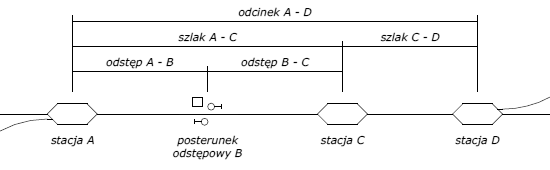
\includegraphics[width=13cm]{skryptkierownik-img/skryptkierownik-img001.png}
		\caption{Podział sieci kolejowej na odcinki, szlaki i odstępy (wg https://www.bsk.isdr.pl/siec.php)}
		\label{fig:siec}
	\end{figure*}


\textbf{Posterunek zapowiadawczy} - jest to posterunek mający możliwość zmiany kolejności jazdy pociągów wyprawianych na tor szlakowy przyległy do tego posterunku. Do posterunków zapowiadawczych należą stacje i posterunki odgałęźne.

\textbf{Granicę} pomiędzy posterunkiem zapowiadawczym a szlakiem stanowi na liniach jednotorowych semafor wjazdowy tego posterunku. Na liniach dwutorowych jest to miejsce znajdowania się semafora wjazdowego i linia prostopadła do osi torów. Jeśli przy danym torze nie ma semafora wjazdowego, jest to miejsce oddalone o 100m od ostatniego rozjazdu lub skrzyżowania torów.

\textbf{Stacja} - jest to posterunek zapowiadawczy, w obrębie którego, oprócz toru głównego zasadniczego, znajduje się co najmniej jeden tor główny dodatkowy, a pociągi mogą rozpoczynać i kończyć jazdę, krzyżować się i wyprzedzać, jak również zmieniać skład lub kierunek jazdy. Duże stacje mogą być podzielone na rejony stanowiące osobne posterunki zapowiadawcze. Stacja, na której układ torów umożliwia jedynie krzyżowanie i wyprzedzanie pociągów, nazywa się mijanką.

\textbf{Pociąg} - jest to skład wagonów lub innych pojazdów kolejowych sprzęgniętych z czynnym pojazdem trakcyjnym albo pojazd trakcyjny – osygnalizowany i przygotowany do jazdy lub znajdujący się w drodze.

Na stacjach tory kolejowe dzielą się na tory: główne, specjalnego przeznaczenia i boczne.

Tory przystosowane do jazd pociągowych nazywają się \textbf{torami głównymi}. Dzielą się one na tory główne zasadnicze i tory główne dodatkowe. Tory główne będące przedłużeniem torów szlakowych nazywają się torami głównymi \textbf{zasadniczymi}, natomiast pozostałe tory główne torami głównymi \textbf{dodatkowymi}. Do torów specjalnego przeznaczenia należą: żeberka ochronne, tory dojazdowe do bocznic, komunikacyjne, wyciągowe, bocznicowe. Inne tory na stacjach są torami bocznymi.

Tory na szlakach i stacjach określa się liczbami. Na \textbf{szlaku} korzysta się z liczebników głównych (tor nr jeden, tor nr dwa), zaś w stacji liczebnikami porządkowymi (pierwszy, drugi). Numeracja torów na szlakach dwutorowych definiowana jest patrząc od początku linii (km 0,0) ku jej końcowi, gdzie tor prawy jest torem nr 1, zaś tor lewy torem
nr 2.
	\begin{figure*}
	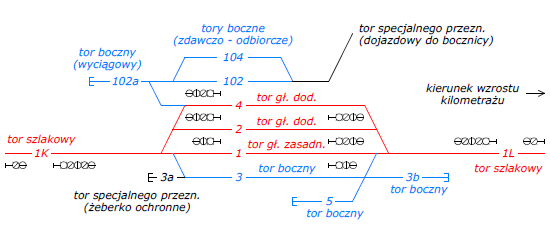
\includegraphics[width=13cm]{skryptkierownik-img/tory-numery.png}
	\caption{Rodzaje torów stacyjnych i ich numeracja (wg https://www.bsk.isdr.pl/siec.php)}
	\label{fig:numeracja-torow}
\end{figure*}

Na \textbf{stacjach} torem nr 1 (pierwszym) jest tor główny zasadniczy będący przedłużeniem toru szlakowego nr 1. Na stacjach węzłowych miarodajną jest linia kolejowa wyższej kategorii, a przy równorzędności linii przyjmuje się linię o większym obciążeniu ruchem pociągów. Kolejne tory stacyjne po \textbf{prawej stronie} toru głównego zasadniczego patrząc od początku linii określa się kolejnymi liczbami \textbf{nieparzystymi}, a znajdujące się po \textbf{lewej} stronie toru głównego zasadniczego kolejnymi liczbami \textbf{parzystymi}. Jeśli tory stacyjne podzielone są na grupy, w sposób ustalony w regulaminie technicznym, dla każdej grupy ustala się osobną dziesiątkę lub setkę liczb.

Przy prowadzeniu ruchu pociągów w ustalonych sytuacjach stosuje się \textbf{telefoniczne zapowiadanie pociągów}, które polega na porozumiewaniu się dyżurnych ruchu za pośrednictwem kablowej łączności telefonicznej. Telefoniczne zapowiadanie pociągów stosuje się zawsze na liniach nie wyposażonych w urządzenia blokady liniowej lub na na liniach kolejowych z blokada liniową w przypadkach, gdy nie jest lub nie może ona być podstawą prowadzenia ruchu. Podstawą prowadzenia pociągu jest między innymi przekazywanie numeru pociągu wyprawianego do kolejnego posterunku następczego. Jeżeli nie wykonują tego urządzenia SRK to stosuje się telefoniczne zapowiadanie pociągów w określonym zakresie dla poszczególnych typów szlaków i urządzeń SRK. 
Na sieci PKP nie ma urządzeń SRK automatycznie przekazujących numer pociągu w związku z czym łączność telefoniczna przy prowadzeniu ruchu pociągów jest stosowana na całej sieci kolejowej.

\section{Budowa toru i rozjazdu}

Nawierzchnia kolejowa oznacza drogę dla pojazdów szynowych. Jest to konstrukcja, składająca się z toru kolejowego lub rozjazdu, po którym poruszają się pojazdy szynowe, elementów podporowych (podkłady lub podrozjazdnice), elementów przytwierdzających i łączących (m.in. złączek) oraz podsypki. Tak jak w przypadku konstrukcji budowlanej, podstawowym zadaniem nawierzchni kolejowej jest przeniesienie obciążenia eksploatacyjnego na podtorze.
Tor kolejowy to dwa toki szynowe ułożone w ustalonej odległości od siebie stanowiące podstawowy układ nośny nawierzchni kolejowej, której układ geometryczny przystosowany jest do bezpiecznego ruchu pojazdów kolejowych, z prędkościami oraz naciskami określonymi poprzez parametry techniczno-eksploatacyjne. Parametry techniczno-eksploatacyjne dla linii kolejowej ustala zarządca infrastruktury, czyli podmiot wykonujący działalność polegającą na zarządzaniu infrastrukturą kolejową na zasadach określonych w ustawie o transporcie kolejowym.
Ze względu na rodzaj konstrukcji nawierzchni, wyróżniamy nawierzchnie podsypkowe (najczęściej stosowane) oraz bezpodsypkowe (stosowane zazwyczaj w tunelach oraz na mostach i wiaduktach). 

\begin{marginfigure}
	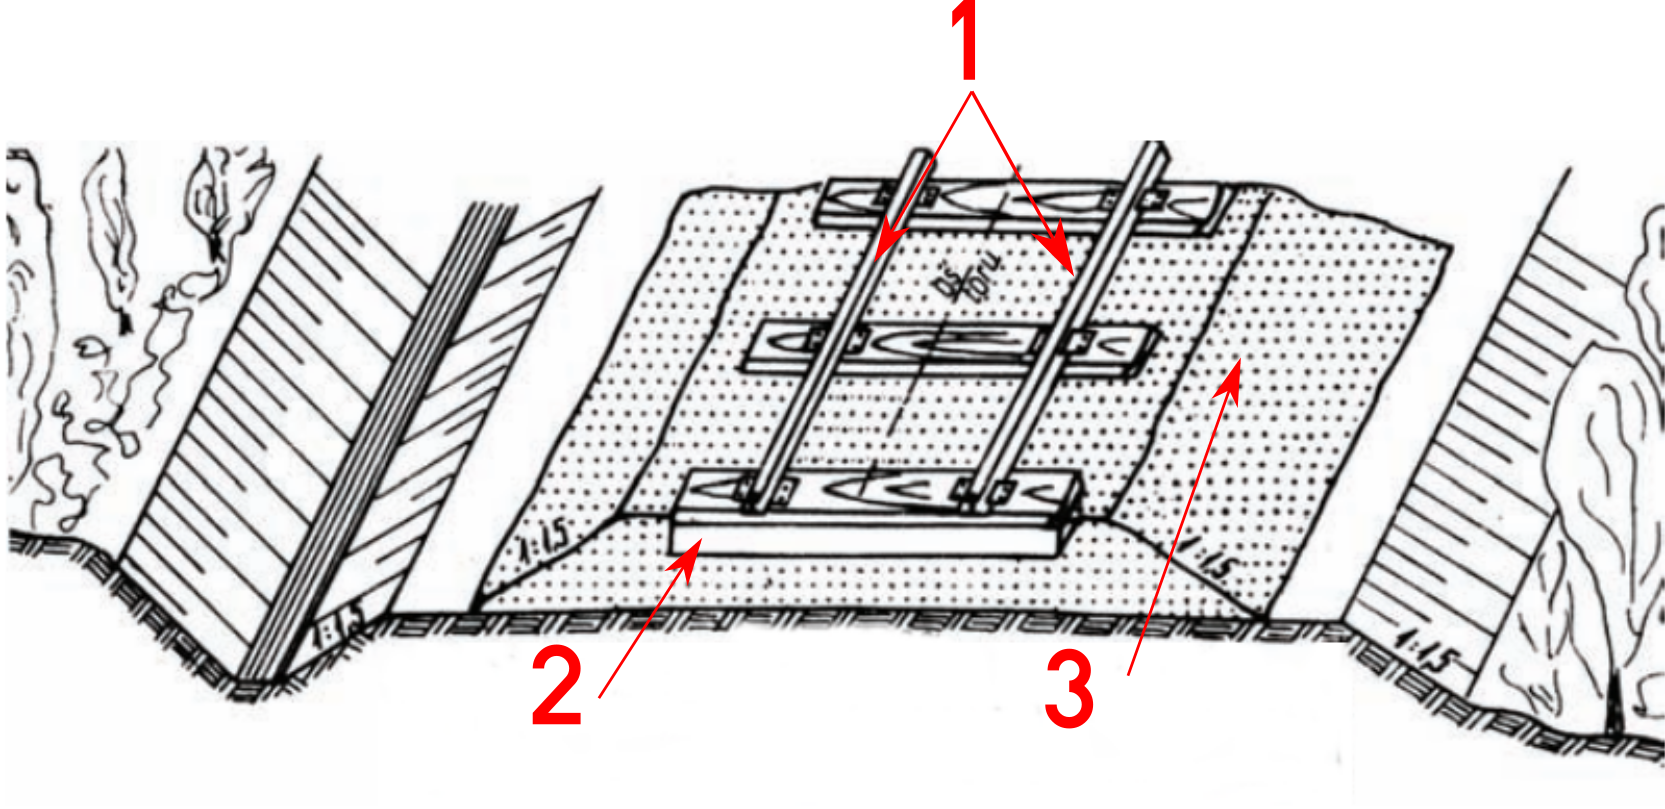
\includegraphics[width=5cm]{skryptkierownik-img/budowa-toru.png}
	\caption{Elementy nawierzchni kolejowej: 1 - szyny, 2 - podkłady, 3 - podsypka,źródło: Drogi Szynowe, Gdańsk 2013}
	\label{fig:tory}
\end{marginfigure}

Nawierzchnia kolejowa składa się z:
\begin{itemize}
\item szyn,
\item systemu przytwierdzeń szyn do podkładów,
\item łączy szynowych i złączek,
\item podkładów,
\item podsypki 
\end{itemize}


Zasadniczą częścią konstrukcji toru kolejowego są szyny. Zadaniem szyn jest przejęcie sił pionowych i poprzecznych z kół taboru i przeniesienie ich na podkłady. Szyny są elementem prowadzącym zestawy kołowe, nadając im właściwy kierunek jazdy. Dodatkowo szyny przewodzą prąd zasilający pojazdy trakcyjne na liniach zelektryfikowanych, są również elementem systemu urządzeń sterowania ruchem kolejowym (odcinki izolowane). W Polsce zasadniczo stosuje się trzy typy szyn kolejowych oznaczonych symbolami S42, S49 (49E1)
oraz UIC60 (60E1).

Tor kolejowy może być wykonany jako klasyczny lub bezstykowy. Tor klasyczny stanowi konstrukcję, w której szyny o normatywnej długości są ze sobą połączone na stałe za pomocą złączek i przytwierdzone do podkładów. Szyny w torze klasycznym połączone są za pomocą złącz:
podpartych na podzłączowych podwójnych podkładach drewnianych z połączeniem szyn łubkami i czterema śrubami łubkowymi;
wiszących z połączeniem szyn łubkami wzmocnionymi i sześcioma śrubami łubkowymi 

Tor bezstykowy stanowi konstrukcję, w której kolejne szyny łączone są ze sobą trwale przy pomocy
zgrzewania elektrooporowego, spawania termitowego lub łukowego. Długość odcinka toru
bezstykowego jest nieograniczona. Odcinki toru z szynami spawanymi lub zgrzewanymi o długości
większej niż 180 m uważa się za tor bezstykowy. Do budowy toru bezstykowego w torach na szlakach
i głównych zasadniczych stosuje się szyny długie zgrzewane stacjonarnie. Łączenie szyn długich oraz
szyn w pozostałych torach powinna być wykonana metodą zgrzewania, spawania termitowego
lub inną metodą dopuszczoną do stosowania przez zarządcę infrastruktury. 

Rozjazd kolejowy to specjalna konstrukcja wielotorowa wykonana z szyn kolejowych,
kształtowników stalowych oraz innych elementów, która umożliwia przejazd pojazdów kolejowych
z jednego toru na drugi z określoną prędkością.
Rozjazd zwyczajny składa się z trzech podstawowych zespołów/bloków, tj.:
A – zwrotnicy, służącej do kierowania zestawów kołowych pojazdu kolejowego
z jednego toru na drugi tor,
B – szyn łączących,
C – krzyżownicy z kierownicami i szynami tocznymi, stanowiącej przecięcie szyn dwóch torów (w tym dziób krzyżownicy i szyny skrzydełkowe)

\begin{figure}
	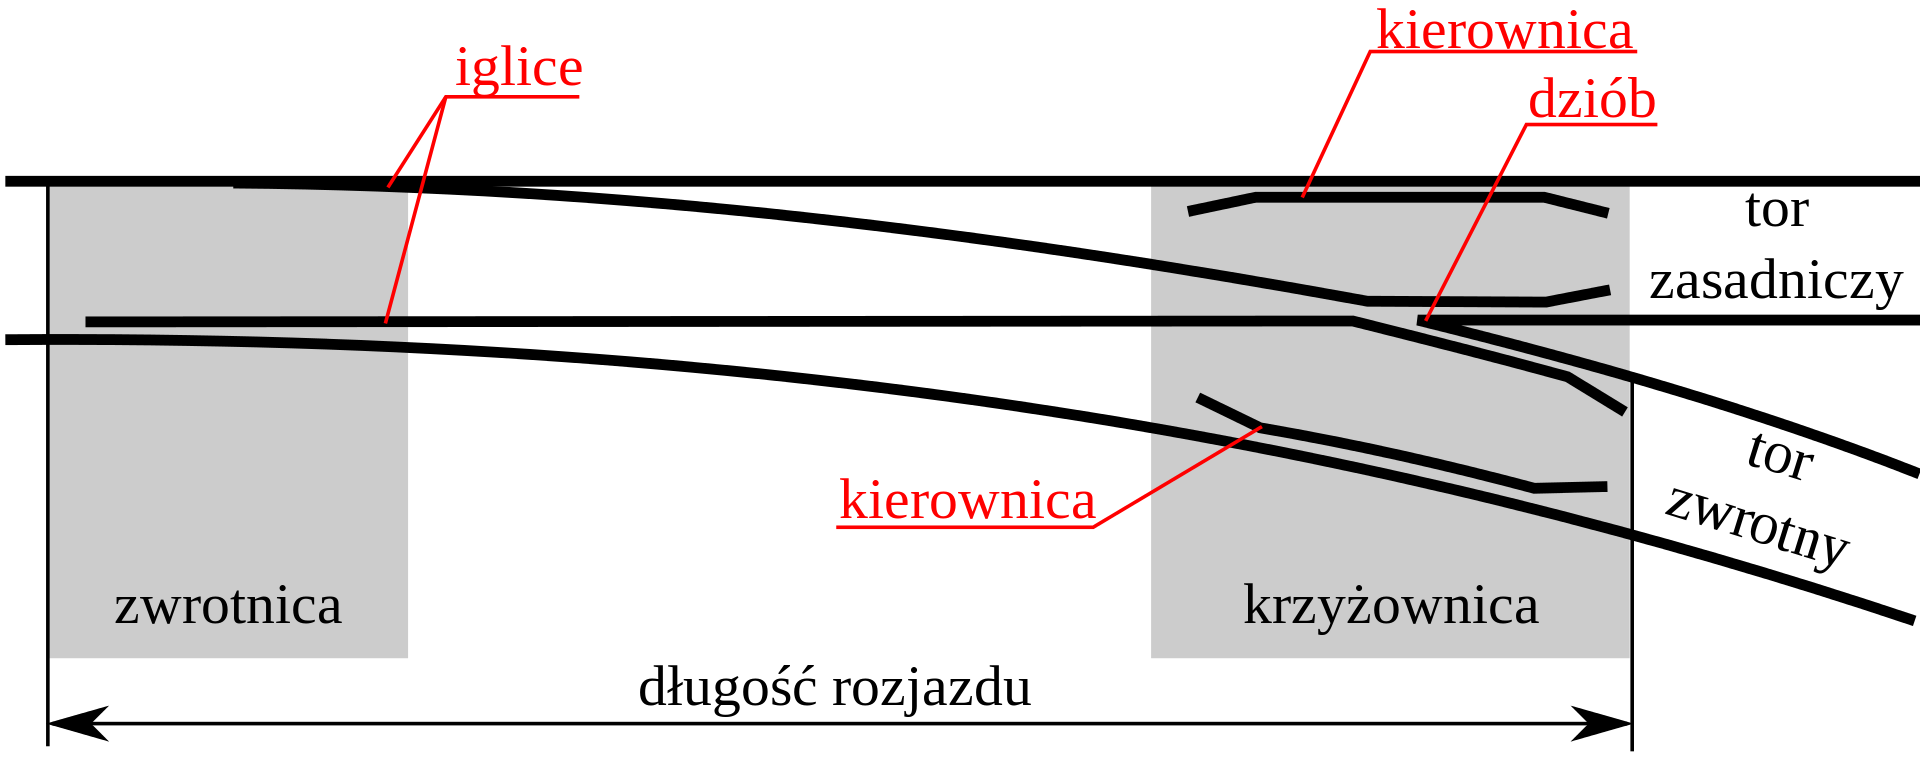
\includegraphics[width=12cm]{skryptkierownik-img/rozjazd.png}
	\caption{Elementy rozjazdu, źródło: Krzysztof Zajaczkowski - pl.wikipedia.org: ''Plik:Bud\_rozjazdu.jpg'', GFDL}
	\label{fig:rozjazd}
\end{figure}
Zwrotnica rozjazdu to jego część, zawierająca elementy ruchome, umożliwiająca przejazd pojazdu
kolejowego z jednego toru na drugi przy zachowaniu ciągłości toków szynowych.
Zwrotnica w rozjeździe zwyczajnym składa się z: opornicy prostej, iglicy łukowej, iglicy prostej, opornicy łukowej.
W celu umożliwienia przestawiania zwrotnic, a jednocześnie dla zapewnienia prawidłowego
przylegania iglicy do opornicy i niedopuszczenia do samoczynnego odsunięcia się iglicy od opornicy
pod przejeżdżającym taborem, stosuje się zamknięcia nastawcze.
Wyróżnia się następujące zamknięcia nastawcze:
\begin{itemize}
	\item hakowe,
	\item suwakowe,
	\item specjalne – pozostałe rodzaje zamknięć nastawczych, różniące się od standardu
	konstrukcyjnego ww. zamknięć nastawczych, np. VCC, HRS, Spherolock, Hydrostar.
\end{itemize}

Zamknięcie nastawcze hakowe znajduje się przy początku iglic i umieszczone jest zazwyczaj między 2 i 3 podrozjazdnicą.
Zamknięcie hakowe jest rozpruwalne, to znaczy, że przy jeździe po zwrotnicy nastawionej do innej jazdy, zwrotnica może być przestawiona przez koła pojazdu podczas ruchu w kierunku zbieżnym (od krzyżownicy ku zwrotnicy) bez uszkodzenia konstrukcji zamknięcia nastawczego.

Jeżeli należy zabezpieczyć rozjazd przed przypadkowym przełożeniem (np. w trakcie awarii), można wykorzystać zamek trzpieniowy - do zabezpieczenia iglicy odlegającej, lub sponę iglicową do zabezpieczenia iglicy przylegającej. Miejsce montażu zamka lub spony jest pomalowane na bocznej ścianie szyny na biało.

W sytuacji rozprucia rozjazdu (wjazd na niepoprawnie ułożony rozjazd od strony krzyżownicy) zabronione jest cofanie składu bo doprowadzi to do wykolejenia. Jeśli konieczne jest ruszenie składem, dopuszczalne to jest wyłącznie do przodu i wyłącznie w sytuacji zagrożenia życia.

Krzyżownica umożliwia swobodny przejazd w jednym poziomie kół pojazdu kolejowego przez miejsce krzyżowania się szyn.
Zespół krzyżownic w rozjeździe zwyczajnym składa się z:
krzyżownicy zwyczajnej, dwóch kierownic, dwóch szyn łączących.
Krzyżownica zwyczajna składa się z dziobnicy, dwóch szyn skrzydłowych i dwóch szyn tocznych z kierownicami. Wewnętrzne toki szynowe przecinających się torów w krzyżownicy tworzą
dziobnicę, która składa się z dzioba i szyn dziobowych. Dziób krzyżownicy jest to środkowy element
krzyżownicy tworzący przednią część dziobnicy. Kierownica wraz z szyną toczną oraz elementami
mocującymi tworzy tzw. urządzenie kierownicy.

Szyny o specjalnym profilu wraz z szynami tocznymi, ułożone naprzeciw dzioba krzyżownicy, tworzą kierownicę.
Służy ona do bezpiecznego przeprowadzenia zestawu kołowego przez obszar krzyżownicy, w którym występuje nieciągłość toków szynowych.  Zestaw kołowy, przechodząc przez krzyżownicę, ociera się wewnętrzną
powierzchnią obrzeża o boczną powierzchnię kierownicy i dzięki temu nastawia obrzeże drugiego koła zestawu kołowego we właściwym kierunku. Dzięki temu krzyżownice zwyczajne nie mają odcinków pozbawionych prowadzenia zestawów kołowych.

Jeżeli rozjazd jest ustawiany ręcznie, to przeciwwaga jest pomalowana na dwa kolory, czarny i biały, oznaczające położenie kierunku jazdy. Kolor biały oznacza kierunek zasadniczy (+). Jeżeli na przeciwwadze w części białej znajdują się dwa czerwone paski, to dozwolona jest obsługa rozjazdu przez drużynę manewrową.

Istnieje możliwość sterowania pracą rozjazdu w sposób mechaniczny z wykorzystaniem dźwigni nastawczych, naprężaczy i drutów pędniowych, lub elektryczny (silnik).

(więcej ilustracji https://utk.gov.pl/download/1/41355/Poradnikdlakomisjikolejowych-toryrozjazdyiskrzyzowaniatorow.pdf)

\section{Przygotowanie pociągu do drogi}

Przed wyprawieniem pociągu w drogę, należy go przygotować do jazdy. W zakres przygotowania wchodzą następujące czynności:

\begin{enumerate}
\item zestawienie zgodne z parametrami określonymi w wewnętrznym rozkładzie jazdy pociągów,
\item wykonanie oględzin technicznych, o ile są wymagane
\item wykonanie wymaganej próby hamulca
\item osygnalizowanie pociągu
\item sprawdzenie czy nie ma przeszkód pod kołami pociągu (dotyczy płozów hamulcowych, czy nie zamknięto wykolejnicy,
etc.) i czy jego hamulce ręczne oraz postojowe są odhamowane
\item posiadanie dokumentów określonych odrębnymi przepisami, które powinny się znajdować w pojeździe kolejowym (wg. przepisów wew. KŚL są to książka pojazdu z napędem, karta próby hamulca, które powinny się znajdować w czynnej kabinie maszynisty, oraz wykaz pojazdów kolejowych w składzie pociągu - u kierownika pociągu)
\end{enumerate}
Po przygotowaniu pociągu do drogi i jego poprawnym osygnalizowaniu należy zgłosić gotowość pociągu do odjazdu.Zgłoszenia dyżurnemu ruchu dokonuje wskazany w regulaminie technicznym pracownik przewoźnika (maszynista lub kierownik pociągu) podając numer pociągu, numer i serię pojazdu trakcyjnego, długość pociągu w metrach, masę ogólną pociągu, informację o TWR, towarach niebezpiecznych lub przesyłkach nadzwyczajnych, oraz podając numer zgody, godzinę zgłoszenia i nazwisko zgłaszającego. Przed odjazdem pociągu dyżurny ruchu powinien przekazać obsadzie pociągu informacje, polecenia i zezwolenia (rozkazy pisemne).

\begin{tcolorbox}
	\begin{enumerate}
		\item Pociągiem nazywa się:
		\begin{enumerate}
			\item Skład sprzęgnięty z czynnym pojazdem trakcyjnym lub pojazd trakcyjny osygnalizowany i przygotowany do drogi lub znajdujący się w drodze,
			\item Skład wagonów sprzęgniętych ze sobą wystawiony na tory odjazdowe bez czynnego pojazdu trakcyjnego,
			\item Pojazd pomocniczy znajdujący się na torach odjazdowych.
		\end{enumerate}
	\end{enumerate}
\end{tcolorbox}

\chapter{Regulaminy techniczne posterunków i odcinków zdalnego prowadzenia ruchu}

Regulamin techniczny stacji i posterunku składa się z tzw. działek które opisują:
\begin{itemize}
	\item położenie posterunku ruchu na linii (wraz z opisem typu blokady liniowej)
	\item sposób prowadzenia ruchu na przyległych szlakach (przy pomocy blokady liniowej lub telefonicznego zapowiadania)
	\item wykaz posterunków technicznych (nastawczych, zwrotniczowskich) na stacji z opisem rodzaju urządzeń oraz granic okręgów nastawczych
	\item skrajnie budowli na przyległych szlakach
	\item przejazdy i przejścia na przyległych szlakach z opisem kategorii, oraz dodatkowymi zaleceniami
	\item wykaz torów stacyjnych, z ich numeracją, opisem przeznaczenia, długością użyteczną, możliwością przejazdu przekroczonej skrajni.
	\item wykaz rozjazdów z opisem położenia zasadniczego, sposobu nastawiania
	\item przyjmowanie i wyprawianie pociągów z towarami niebezpiecznymi, TWR i przesyłkami nadzwyczajnymi oraz sposób postępowania przy sytuacjach awaryjnych
	\item opis przebiegów pociągowych i manewrowych dla wjazdu i wyjazdów
	\item środki pomocnicze dla zabezpieczania w przypadku ''Sz'' lub innych sytuacji nietypowej
	\item sposób zabezpieczania przed zbiegnięciem pojazdów odstawionych na postój (\textbf{dz.42})
	\item sposób zgłoszenia gotowości do odjazdu pociągu
	\item regulaminy bocznic, sposoby prowadzenia jazd trakcyjnych, etc.
	\item plan schematyczny posterunku
\end{itemize}
	\begin{marginfigure}
	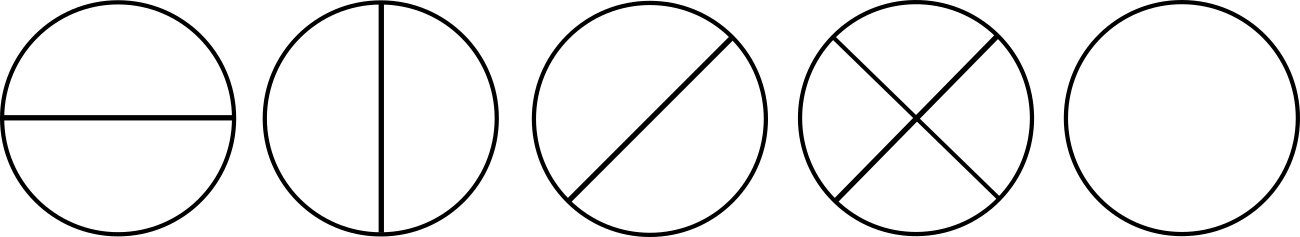
\includegraphics[width=5.5cm]{skryptkierownik-img/komory_sygnalowe_pl.png}
	\caption{Symbole komór sygnałowych, od lewej czerwona, zielona, pomarańczowa, niebieska, matowobiała}
\end{marginfigure}

Na planach schematycznych posterunków ruchu używa się znormalizowanych symboli oznaczających cechy urządzeń SRK oraz podawanych sygnałów na sygnalizatorach.

\chapter{Rodzaje urządzeń sterowania ruchem kolejowym i łączności}

Blokada stacyjna uzależnia nastawnie tego samego posterunku ruchu, czyli na przykład w obrębie stacji, a blokada liniowa są to urządzenia techniczne przeznaczone do regulacji następstwa pociągów oraz ustalenia kierunku ruchu na szlaku (uzależnienie czynności nastawni sąsiednich posterunków ruchu). 

\textbf{Półsamoczynne blokady liniowe} uniemożliwiają wyprawienie pociągu na szlak (odstęp) do czasu potwierdzenia przybycia w całości poprzedniego pociągu do następnego posterunku ruchu. Z reguły potwierdzenie to dawane jest przez personel ruchu, po wzrokowym stwierdzeniu, że pociąg wjechał z sygnałami końca pociągu, a sygnały zezwalające na semaforach podawane są ręcznie. Konieczność obsady posterunków odstępowych powodowała, że szlaki z półsamoczynną blokadą liniową rzadko dzielono na odstępy.

Na szlakach z półsamoczynną blokadą liniową ruch pociągów regulowany jest w oparciu o blokowanie i zwalnianie blokady. Sygnał zezwalający na wyjazd na szlak (odstęp) może być podany tylko jeden raz do czasu zwolnienia blokady. Zmiany stanu blokady są jednocześnie informacją dla personelu o wyprawieniu lub przyjęciu pociągu przez sąsiedni posterunek ruchu.

\textbf{Samoczynne blokady liniowe} wyposażone są w układową kontrolę niezajętości odstępów, a sygnały na semaforach odstępowych wyświetlane są samoczynnie, w zależności od sytuacji ruchowej. Odstępy samoczynnej blokady liniowej są krótkie, co pozwala na uzyskanie dużej przepustowości.

Przy samoczynnej blokadzie liniowej ruch pociągów regulowany jest na podstawie kontroli niezajętości odstępów blokowych przez obwody torowe lub liczniki osi. Na szlaku stosowane są samoczynne semafory odstępowe, na których sygnały wyświetlane są samoczynnie, zależnie od sytuacji ruchowej i ustawionego kierunku ruchu. Prowadzenie ruchu pociągów, poza zmianą kierunku ruchu, nie wymaga obsługi urządzeń blokady.

Na szlaku jednotorowym dwukierunkowym wyposażonym w SBL, jak na każdym szlaku jednotorowym, jest ustalony jeden kierunek ruchu, jako uprzywilejowany. Najczęściej jest to kierunek zgodny ze wzrastającym kilometrowaniem na linii. Według tego kierunku jest ustalony stan zasadniczy blokady liniowej (każdego typu). 
Jeżeli SBL znajduje się w stanie zasadniczym (szlak jest wolny) to świecą się semafory kierunku uprzywilejowanego, natomiast dla kierunku przeciwnego semafory są wygaszone, z wyjątkiem ostatniego semafora SBL ze wskaźnikami W18, który zawsze jest oświetlony. 
Przełączenie kierunku ruchu następuje po telefonicznym porozumieniu dyżurnych ruchu sąsiednich posterunków ruchu i po obsłużeniu odpowiednich manipulatorów blokady (żądania pozwolenia, dania pozwolenia) według ustalonych zasad obsługi tych urządzeń - sytuacja podobna do tej z PBL. 

Blokady liniowe \textbf{jednokierunkowe} przeznaczone są dla szlaków dwutorowych i ich działanie ogranicza się do regulacji następstwa ruchu pociągów w jednym kierunku. Przebiegi na tory szlakowe w kierunku przeciwnym do zasadniczego nie są przewidziane lub są nieuzależnione od stanu blokady liniowej.

Blokady liniowe \textbf{dwukierunkowe} umożliwiają prowadzenie ruchu pociągów po torze szlakowym w obu kierunkach. Ustawienie wybranego kierunku ruchu wymaga przeważnie dania pozwolenia przez personel posterunku zapowiadawczego mającego przyjąć pociąg. W przypadku obsługi blokady liniowej przez nastawnię wykonawczą, danie pozwolenia powinno być uzależnione od otrzymania polecenia od dyżurnego ruchu, przekazanego przez urządzenia (otrzymanie zlecenia). W niektórych typach blokad liniowych dwukierunkowych, poza stanem ustawionego kierunku ruchu występować może stan neutralny, w którym żaden z kierunków nie jest włączony.

 


\chapter{Sygnalizacja kolejowa}

\section{Wskaźniki}

\begin{center}
	\begin{figure*}
		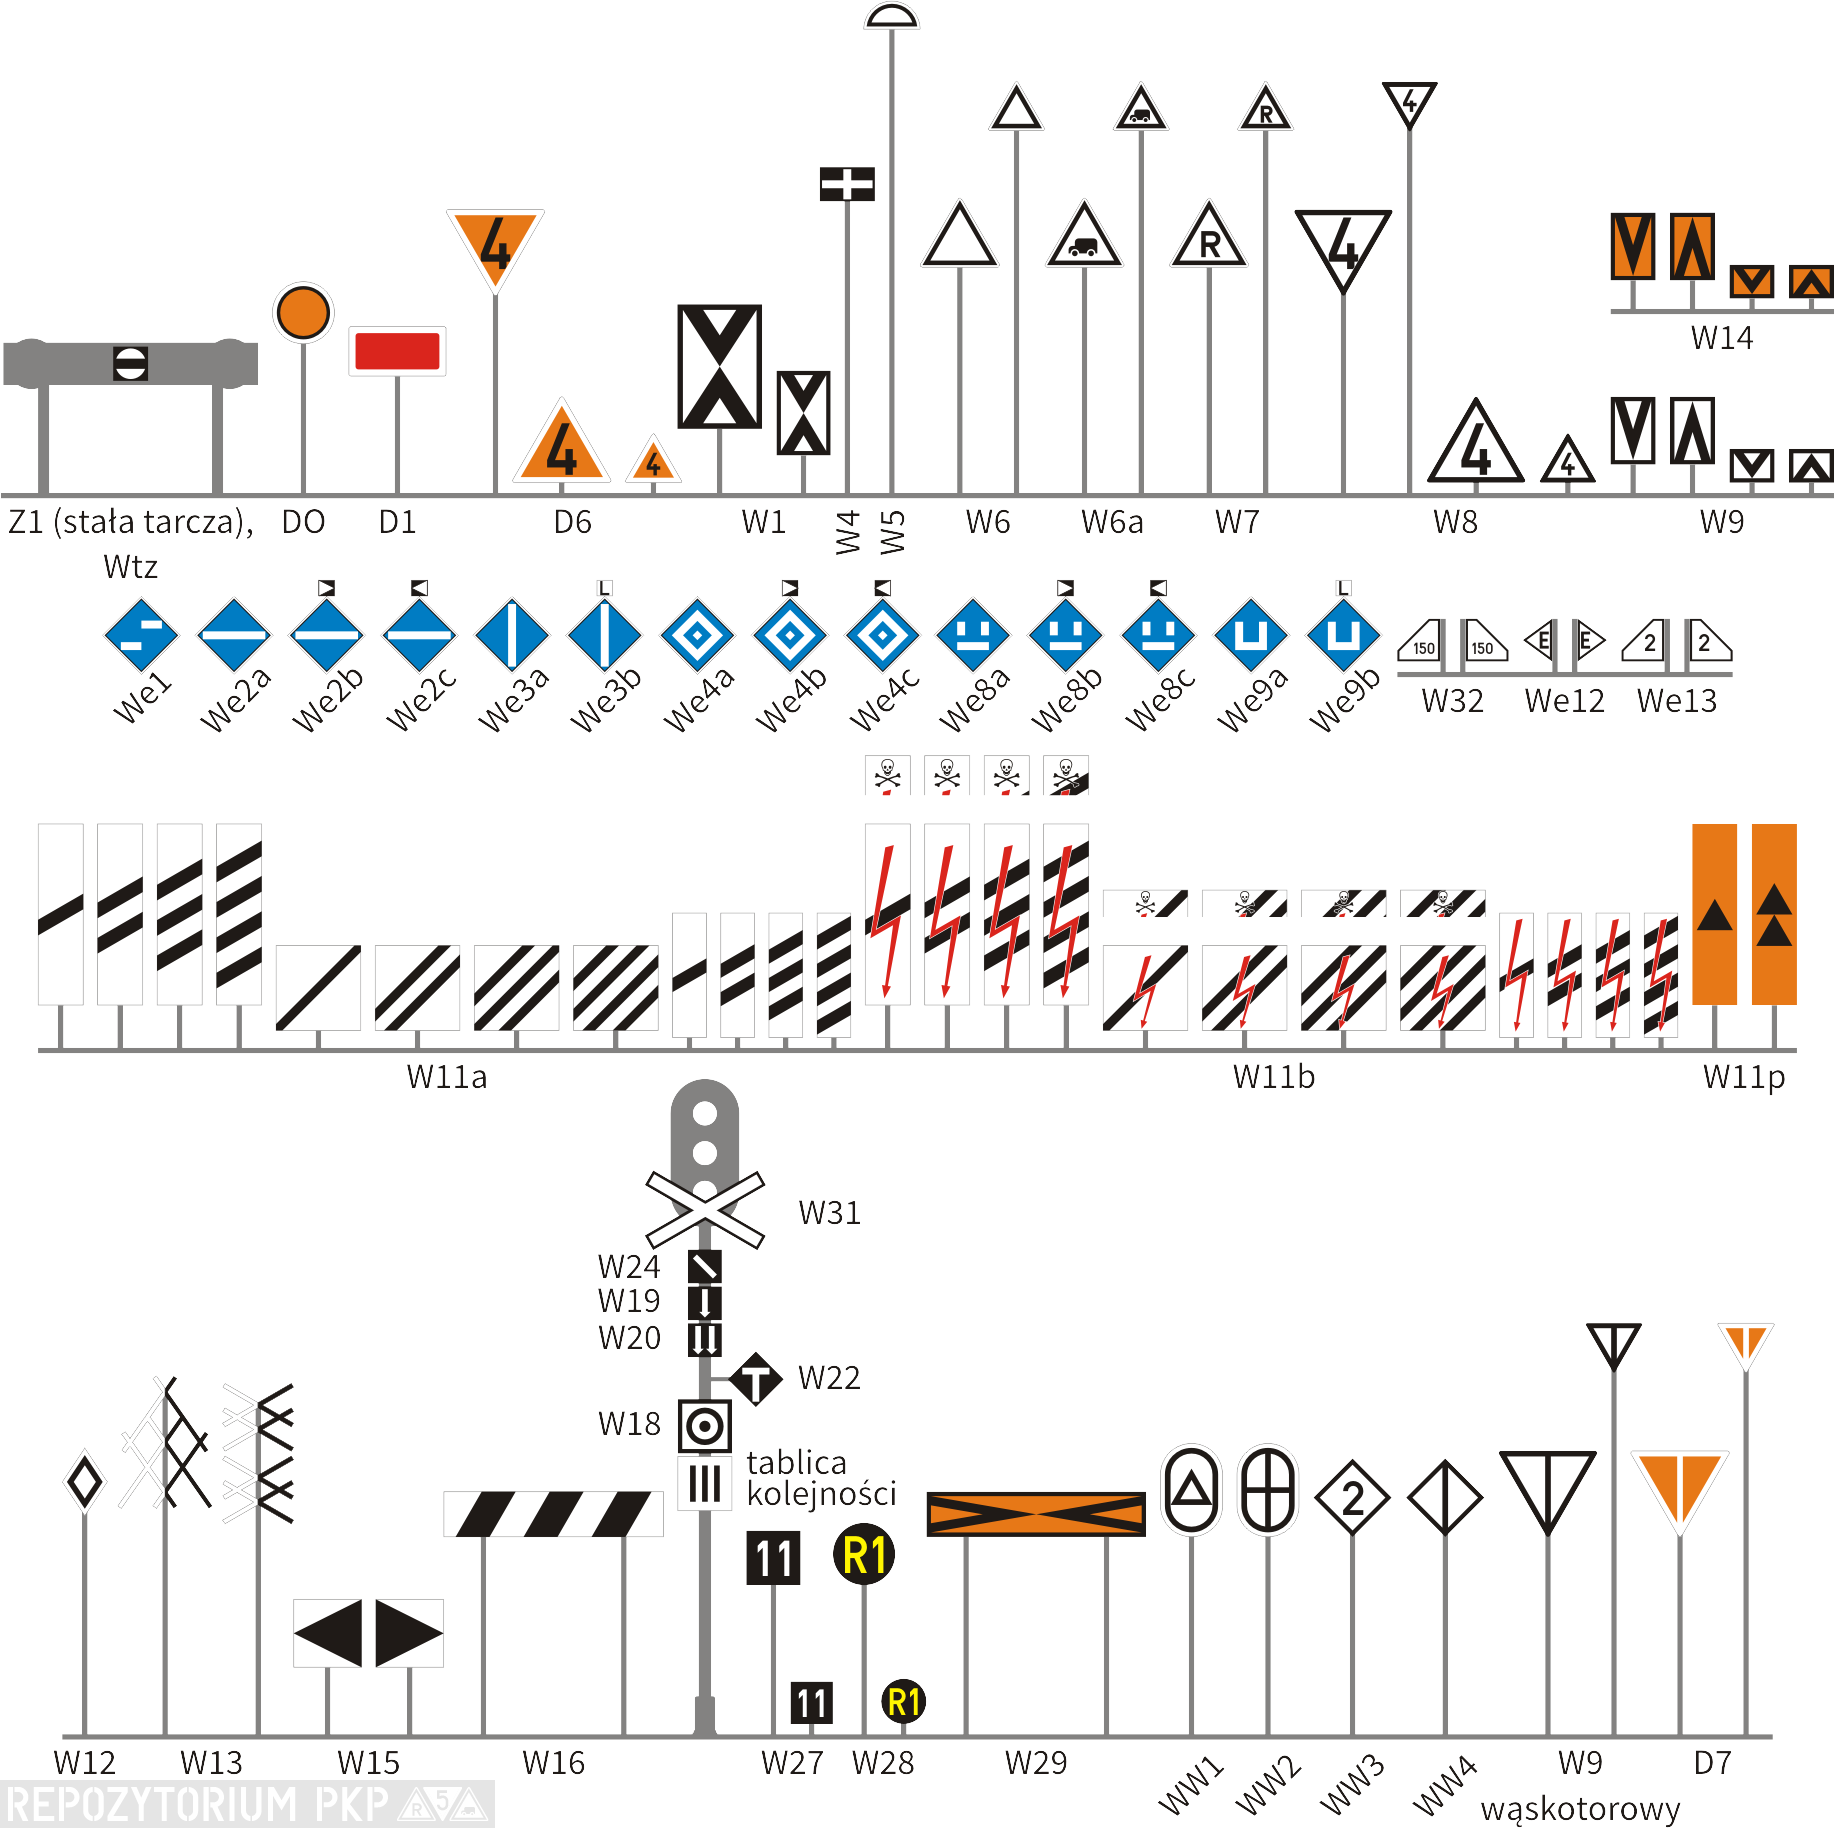
\includegraphics[width=16cm]{skryptkierownik-img/skryptkierownik-img003.png}
		\caption{Wskaźniki przytorowe (wg http://pkprepo.net/wskazniki-kolejowe-pkp/)}
		\label{fig:wskazniki}
	\end{figure*}
\end{center}

\subsection{W1 - wskaźnik usytuowania}

Prostokątna biała tablica z czarnym obramowaniem, a na niej dwa czarne kąty, oparte na krótszych bokach prostokąta, jeden nad drugim, stykające się wierzchołkami w środku tablicy. Wskaźnik W 1 oznacza miejsce ustawienia tarczy ostrzegawczej semaforowej lub przejazdowej, a na szlakach z samoczynną blokadą liniową czterostawną - przedostatniego
semafora odstępowego blokady samoczynnej na szlaku przed semaforem wjazdowym. Wskaźnik W1 stawiany jest bezpośrednio przed tarczą ostrzegawczą kształtową lub świetlną. Informuje, że TO podaje sygnał, jakiego należy spodziewać się na semaforze, do którego się ona odnosi. Dlatego też wskaźnika W1 nie stawia się przed TO nieruchomą.

	\begin{marginfigure}
		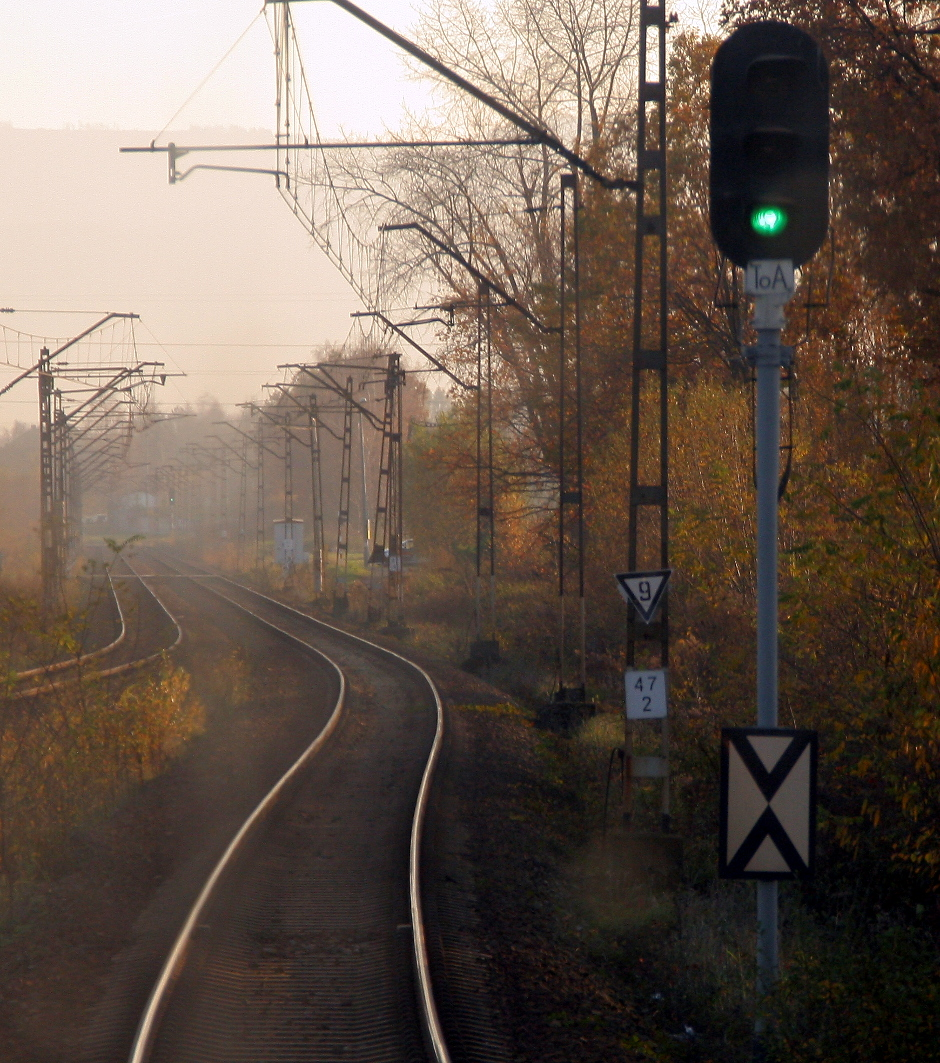
\includegraphics[width=6cm]{skryptkierownik-img/skryptkierownik-img004.jpg}
		\caption{Wskaźnik W1}
	\end{marginfigure}

\subsection{W3 - wskaźnik unieważnienia + W15 wskaźnik zmiany lokalizacji}

Wskaźnik W 3 {\textquotedbl}Wskaźnik unieważnienia{\textquotedbl} oznacza, że znajdujący się z prawej strony toru przy
tym wskaźniku semafor lub tarcza zatrzymania nie odnoszą się do toru, przy którym stoi wskaźnik. Wskaźnik W 3 ustawia
się z prawej strony toru przy znajdującym się tam semaforze lub tarczy zaporowej dla oznaczenia, że semafor ten lub
tarcza zaporowej nie odnoszą się do toru, przy którym stoi wskaźnik. Sygnał dzienny stanowi słup semafora pomalowany na
szaro, zaś sygnał nocny białe światło świecące ciągle na szczycie.

Wskaźnik W 15 {\textquotedbl}Wskaźnik zmiany lokalizacji{\textquotedbl} oznacza, że semafor, sygnalizator powtarzający
lub tarcza ostrzegawcza nie są umieszczone w miejscu, w którym powinny się znajdować, pomimo to odnoszą się do toru,
przy którym stoi wskaźnik. Kwadratowa biała tablica z czarnym trójkątem zwróconym ostrzem w kierunku semafora,
sygnalizatora powtarzającego lub tarczy ostrzegawczej (trójkąt równoramienny, którego podstawą jest bok kwadratu, a
wierzchołek skierowany do sygnalizatora leży na środku przeciwległego boku). Wskaźnik W 15 ustawia się w tym miejscu, w
którym powinny być ustawione: semafor, sygnalizator powtarzający lub tarcza ostrzegawcza.

	\begin{figure*}
		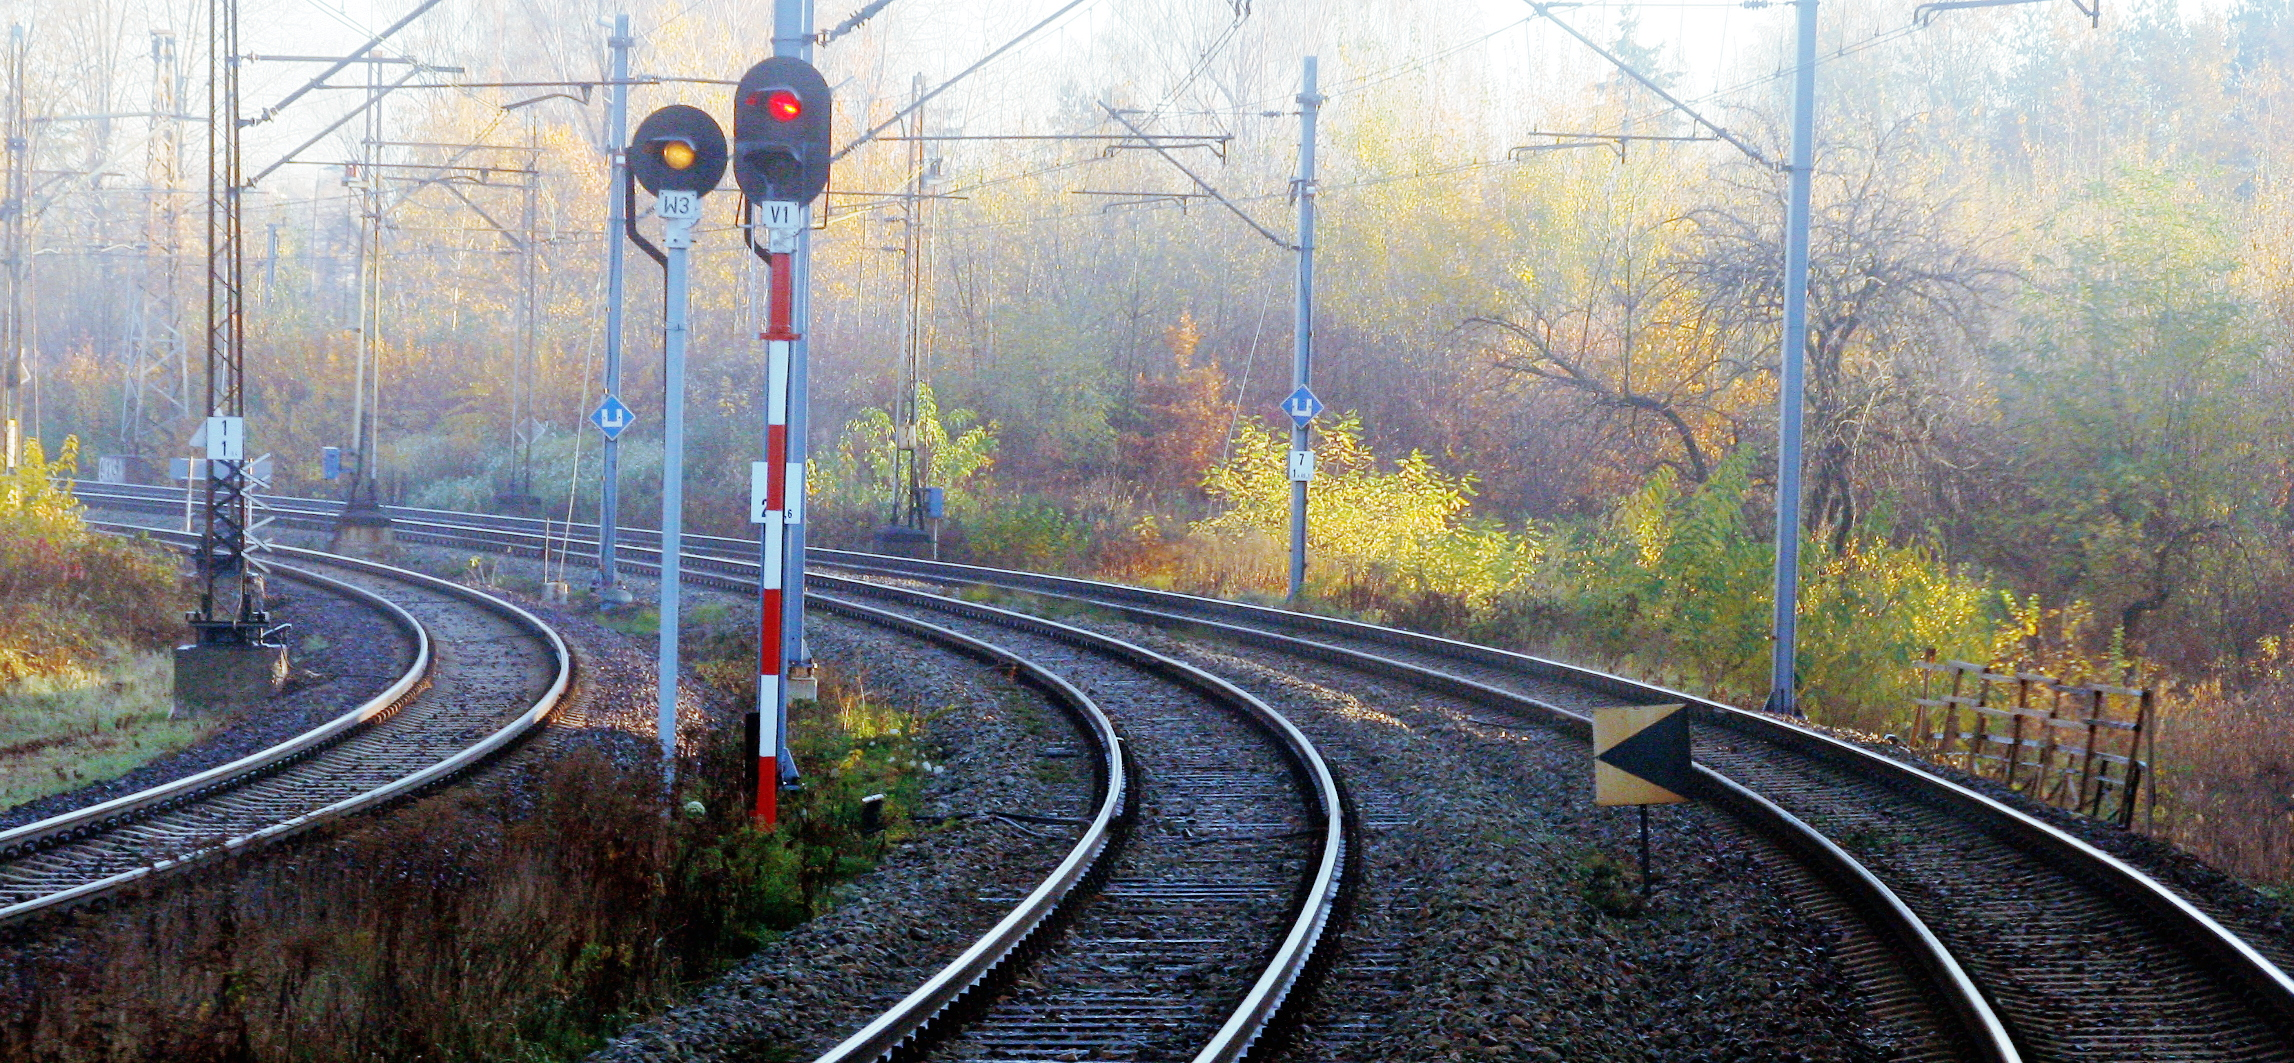
\includegraphics[width=14cm]{skryptkierownik-img/skryptkierownik-img005.jpg}
		\caption{Od lewej: Wskaźnik unieważnienia W3, Semafor wjazdowy odnoszący się do toru środkowego, oraz wskaźnik zmiany lokalizacji W15, st. Katowice Ligota}
	\end{figure*}

\subsection{W4 - wskaźnik zatrzymania}

Wskaźnik służy do oznaczenia miejsca na stacji, przystanku, posterunku osłonnym, do którego może dojechać czoło zatrzymującego się tam pociągu; pociąg mający postój należy zatrzymać w takiej odległości przed wskaźnikiem, aby ruch podróżnych był najdogodniejszy.	
\begin{marginfigure}
	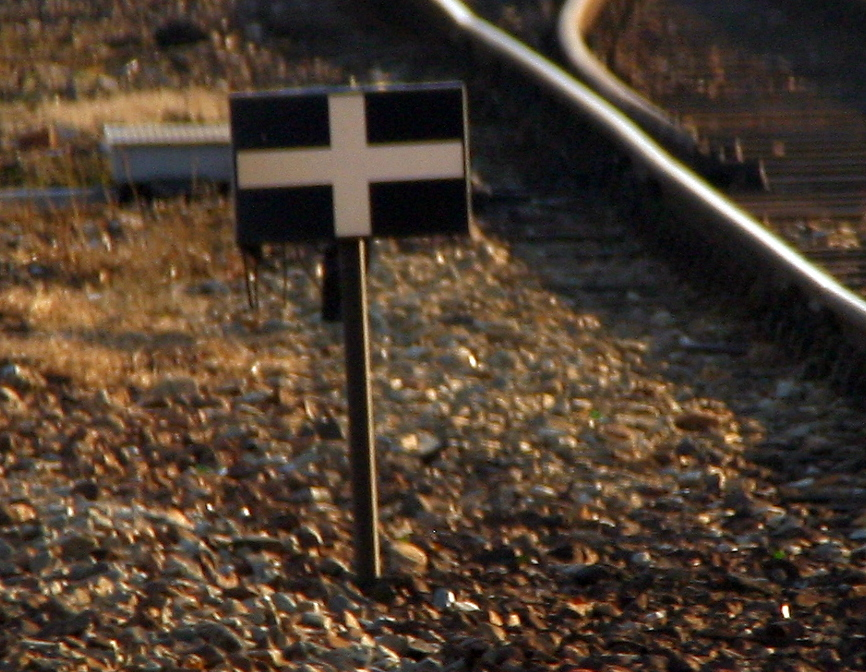
\includegraphics[width=5cm]{skryptkierownik-img/skryptkierownik-img006.jpg}
	\caption{Wskaźnik W4 w międzytorzu}
\end{marginfigure} 
Wskaźnik ustawia się przy końcu peronu lub przed ukresem z prawej strony toru, do którego się odnosi.

\subsection{W32 - wskaźnik czoła pociągu}

Oznacza miejsce zatrzymania czoła pociągu o długości określonej tym wskaźnikiem. Stosuje się go na stacjach i przystankach osobowych. Wskaźnik W 32, w razie potrzeby więcej niż jeden, dla pociągów o różnych długościach, ustawia się, rozmieszczając go w zależności od warunków miejscowych w taki sposób, aby zapewniona została możliwie
najdogodniejsza obsługa podróżnych.
	\begin{marginfigure}
		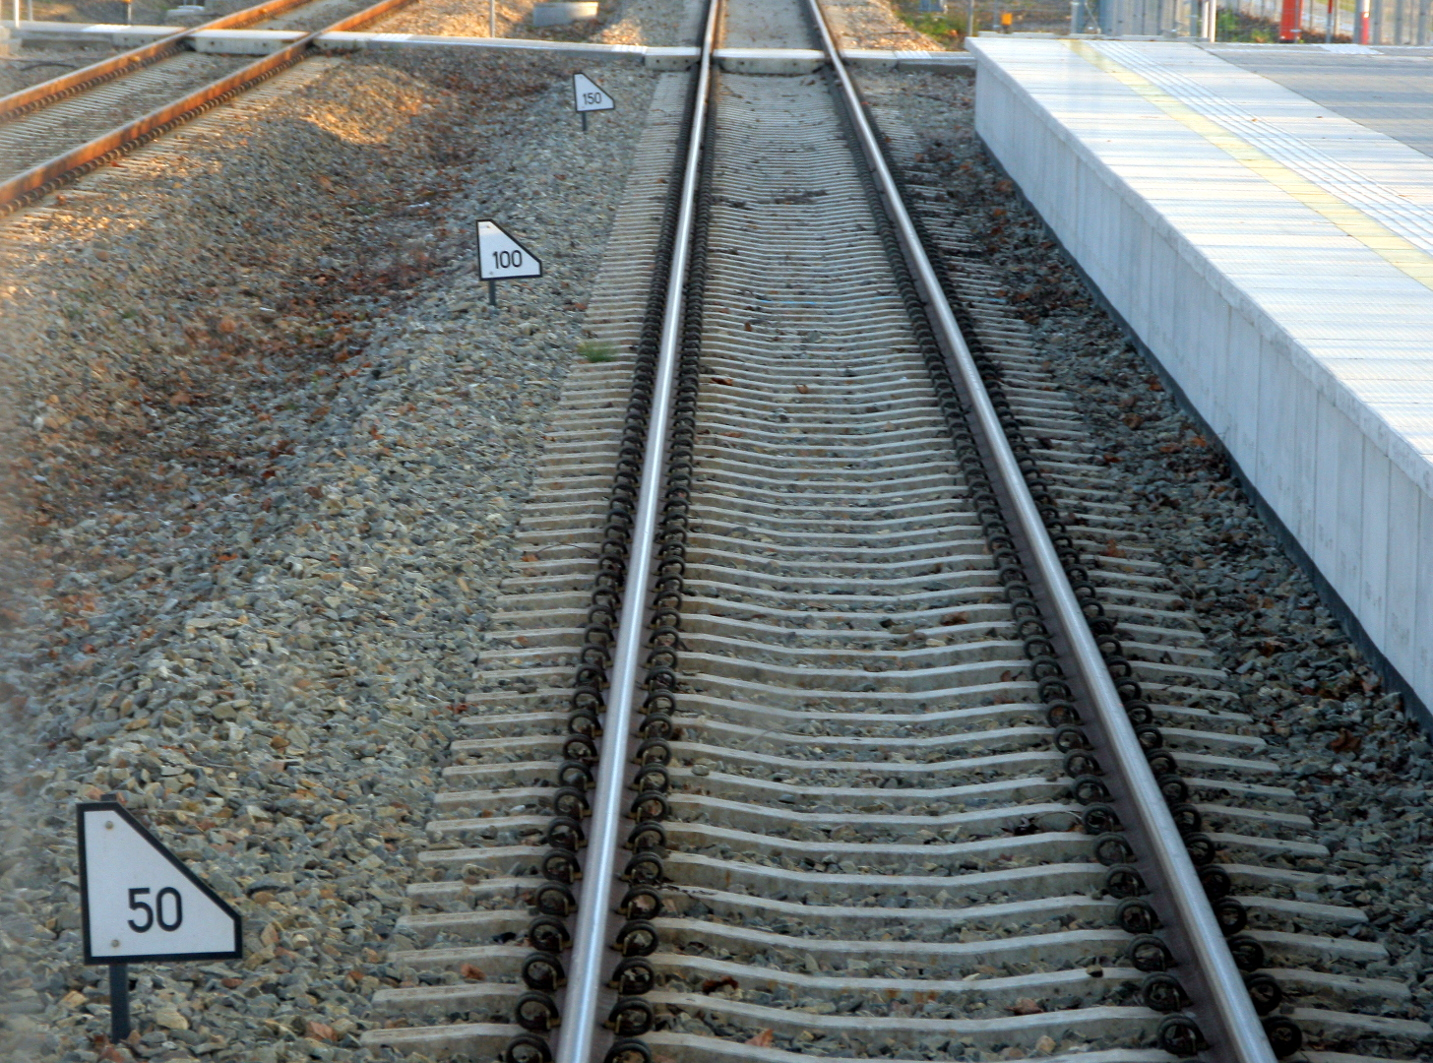
\includegraphics[width=5cm]{skryptkierownik-img/skryptkierownik-img007.jpg}
		\caption{Wskaźniki czoła pociągu W32 w st. Bielsko-Biała Leszczyny}
	\end{marginfigure}

\subsection{W16 - wskaźnik przystanku osobowego}

Wskaźnik W 16 {\textquotedbl}Wskaźnik przystanku osobowego{\textquotedbl} oznacza, że za wskaźnikiem w odległości drogi hamowania znajduje się przystanek osobowy. Wskaźnik W 16 ustawia się skośnie do toru przed przystankami osobowymi, na których nie ma semaforów, z prawej strony toru, do którego się odnosi, w odległości drogi hamowania pociągów obowiązującej na danym szlaku, liczonej od wskaźnika W 4, ustawionego na tym przystanku.
	\begin{marginfigure}
		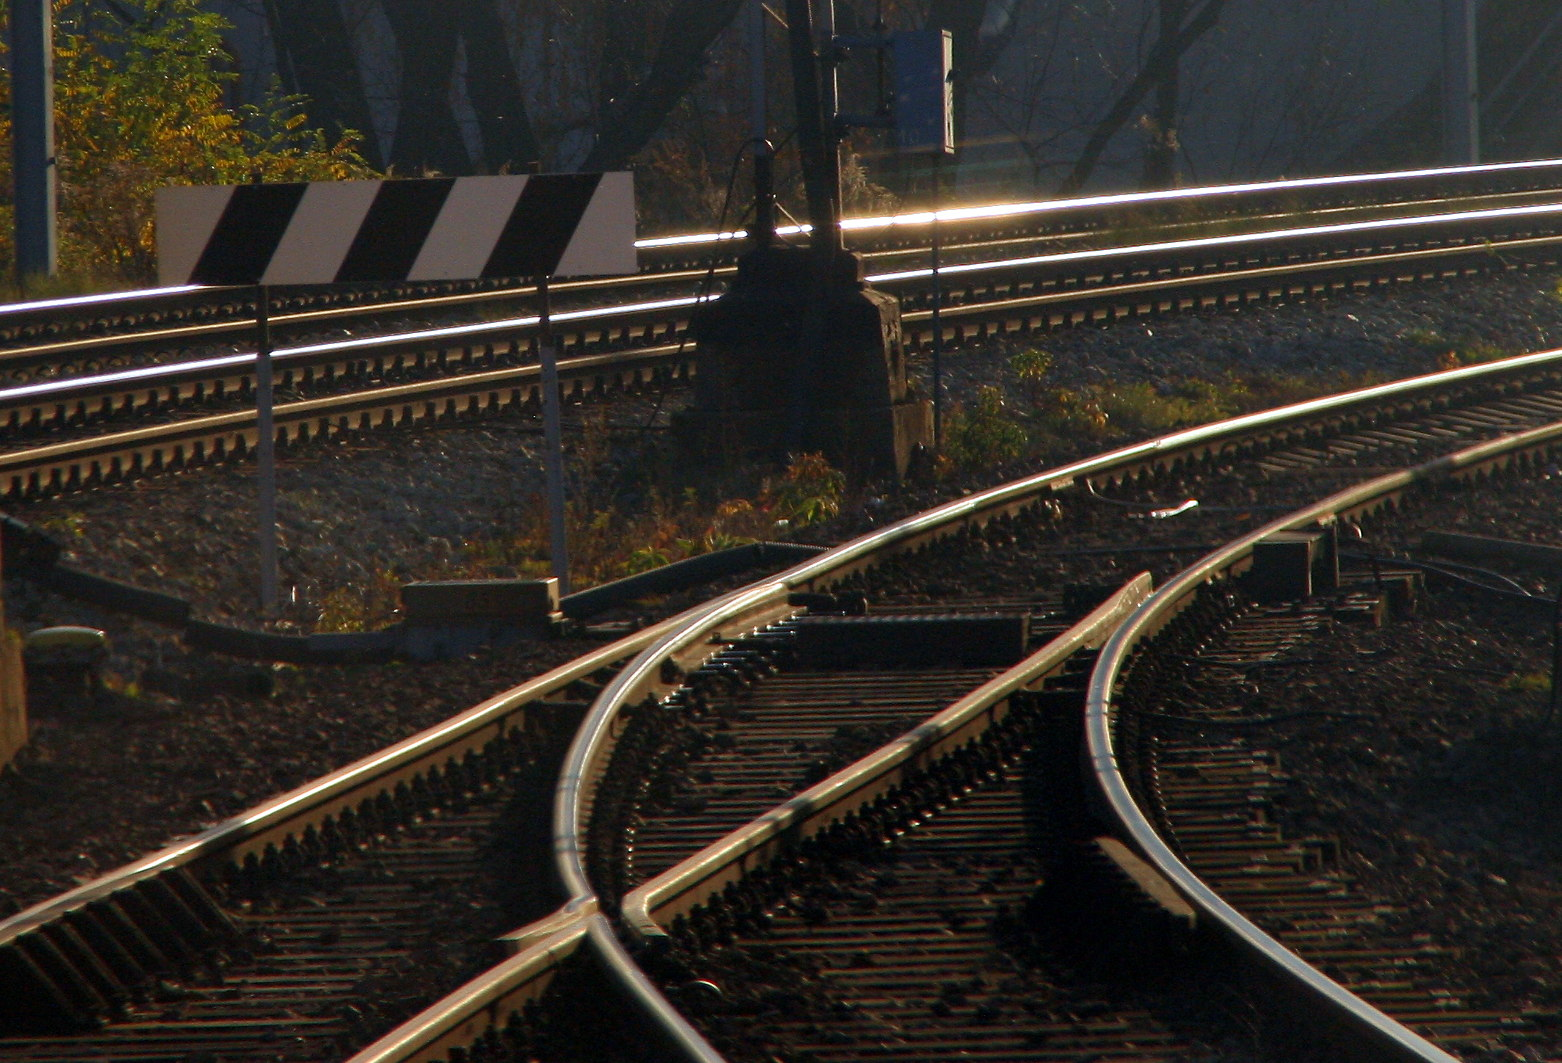
\includegraphics[width=5cm]{skryptkierownik-img/skryptkierownik-img008.jpg}
		\caption{Wskaźnik W16 przed p.o. Katowice Piotrowice}
	\end{marginfigure}

\subsection{W5 - wskaźnik przetaczania}

Wskaźnik stosuje się niezależnie od tarcz manewrowych na tych stacjach i przy tych torach, na których zachodzi potrzeba stałego oznaczenia granicy, do której przetaczanie jest dozwolone; przetaczanie poza wskaźnik dopuszczalne jest tylko za zezwoleniem dyżurnego ruchu. 
	\begin{marginfigure}
	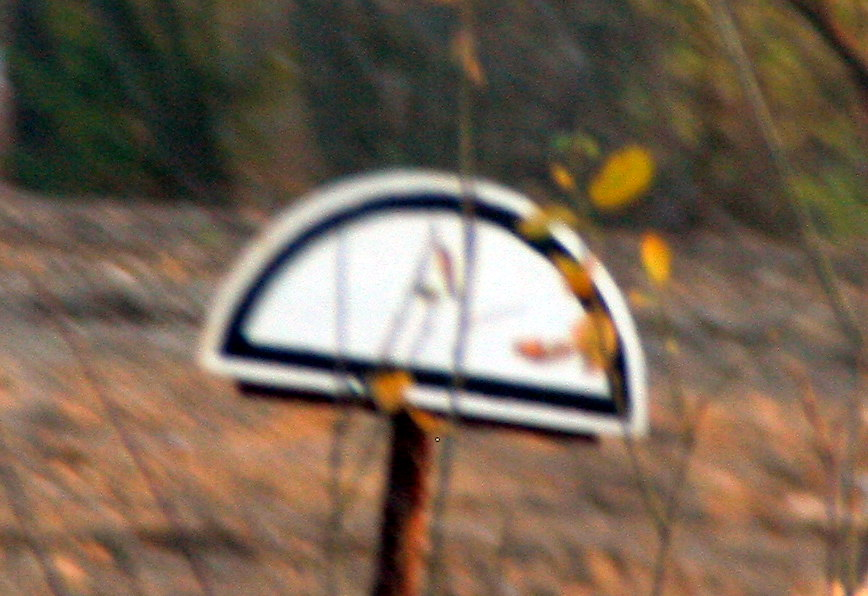
\includegraphics[width=5cm]{skryptkierownik-img/skryptkierownik-img009.jpg}
	\caption{Wskaźnik W5 - granica przetaczania}
\end{marginfigure}
Wskaźnik należy ustawiać przed semaforem wjazdowym w odległości co najmniej 100 m, patrząc w kierunku szlaku, na stacjach linii kolejowych dwutorowych wskaźnik ustawia się przy torach wjazdowych, po stronie semafora wjazdowego, a na stacjach linii kolejowych jednotorowych wskaźnik ustawia się po prawej stronie toru głównego zasadniczego, patrząc w kierunku szlaku.


\subsection{W6, W6a, W6b, W7 - wskaźniki ostrzegania}
	\begin{marginfigure}
	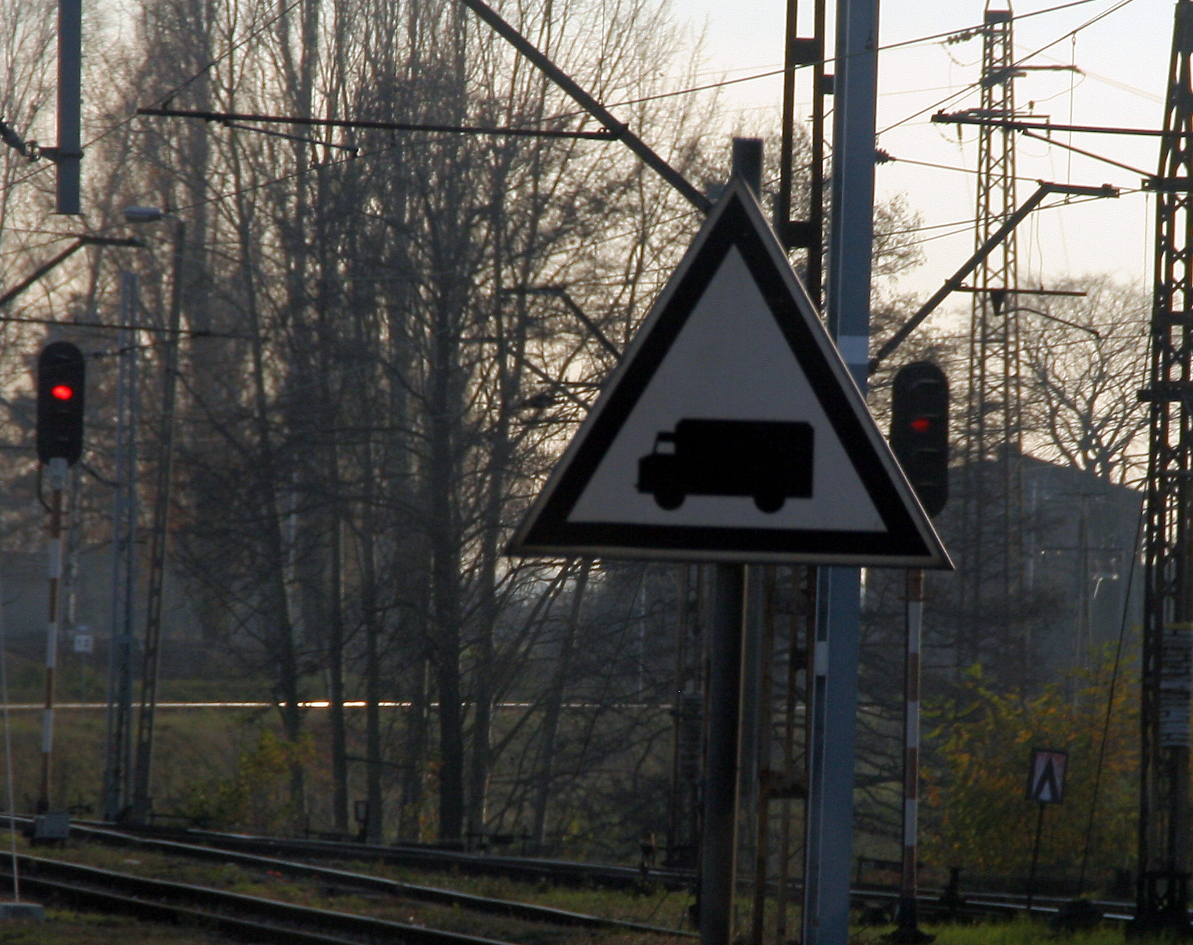
\includegraphics[width=5cm]{skryptkierownik-img/skryptkierownik-img010.jpg}
	\caption{Wskaźnik W6a}
\end{marginfigure}
Wskaźnik W6 wskazuje miejsce w którym należy podać sygnał Rp1 “Baczność”. Wskaźnik W 6a ustawia się przed przejazdami wszystkich kategorii i przejściami kolejowymi według zasad określonych w przepisach o warunkach technicznych, jakim powinny odpowiadać skrzyżowania linii kolejowych z drogami publicznymi i ich usytuowanie. Wskaźnik W6b ustawia się przed przejazdami i przejściami kolejowo-drogowymi, o szczególnym zagrożeniu. Sygnał “Baczność” należy w takim przypadku podawać wielokrotnie. Wskaźnik W7 stosuje się tam, gdzie maszynista powinien dać sygnał {\textquotedbl}Baczność{\textquotedbl} ze względu na bezpieczeństwo ludzi pracujących na torze i ustawia się z obu stron przed miejscem prowadzenia robót na torze, w odległości od 300 do 500 m od miejsca prowadzenia robót, w zależności od warunków miejscowych.
	\begin{marginfigure}
		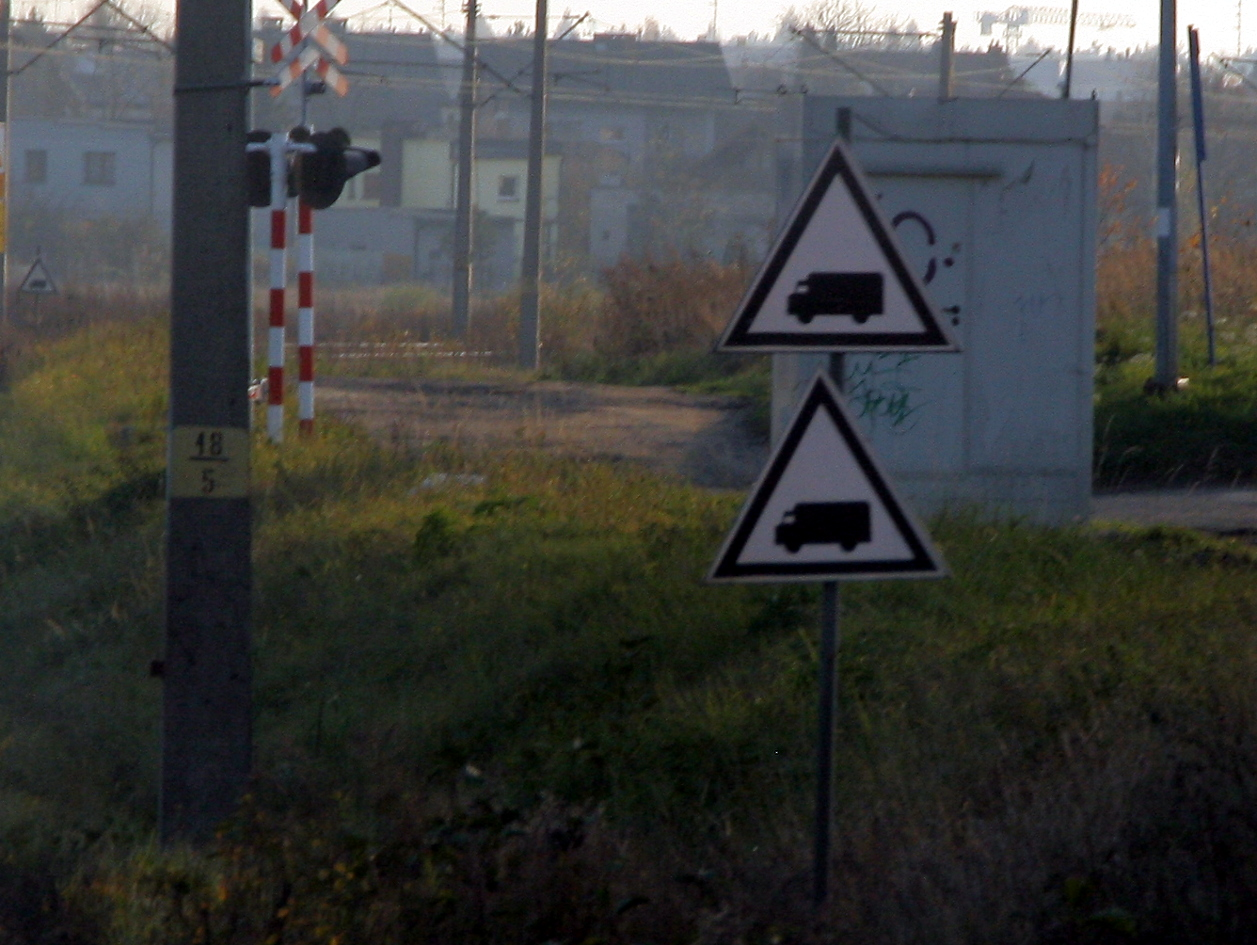
\includegraphics[width=5cm]{skryptkierownik-img/skryptkierownik-img011.jpg}
		\caption{Wskaźnik W6b}
	\end{marginfigure}

\subsection{W8 - wskaźnik ograniczenia prędkości + W9 - wskaźnik odcinka ograniczonej prędkości}

Wskaźnik W 8 {\textquotedbl}Wskaźnik ograniczenia prędkości{\textquotedbl} oznacza, że należy zmniejszyć prędkość jazdy. Trójkątna biała tablica (trójkąt równoboczny) z czarnym obramowaniem, zwrócona wierzchołkiem ku dołowi, a na niej czarna liczba wskazująca dozwoloną prędkość (w dziesiątkach km/h); gdy nie można ustawić tej tablicy z zachowaniem skrajni, stosuje się tablicę zwróconą wierzchołkiem ku górze i umieszczają nisko na wysokości główki szyny. Wskaźnik bez liczby oznacza prędkość 20 km/h. Wskaźnik ustawia się w odległości drogi hamowania obowiązującej na danej linii kolejowej przed początkiem odcinka, po którym należy jechać ze zmniejszoną prędkością; ponadto miejsce to, a w miarę potrzeby także miejsce, od którego wolno powrócić do normalnej prędkości, oznacza się wskaźnikami W9, w obrębie stacji wskaźnik ustawia się na zasadach obowiązujących dla szlaku jednotorowego. 

W przypadku konieczności zmniejszenia prędkości w torach głównych dodatkowych lub na rozjazdach nie leżących w torach głównych zasadniczych nie wymaga się ustawienia wskaźników W8, lecz na początku, a w razie potrzeby i na końcu odcinka, na którym obowiązuje ograniczenie prędkości, ustawia się tylko właściwy wskaźnik W9.

W przypadku konieczności zmniejszenia prędkości pociągów w obrębie stacji na całej jej długości należy ustawić wskaźnik przed stacją, przy tarczy ostrzegawczej odnoszącej się do semafora wjazdowego; w tym przypadku zmniejszenie prędkości obowiązuje do czasu minięcia przez pociąg całej stacji,
	\begin{marginfigure}
	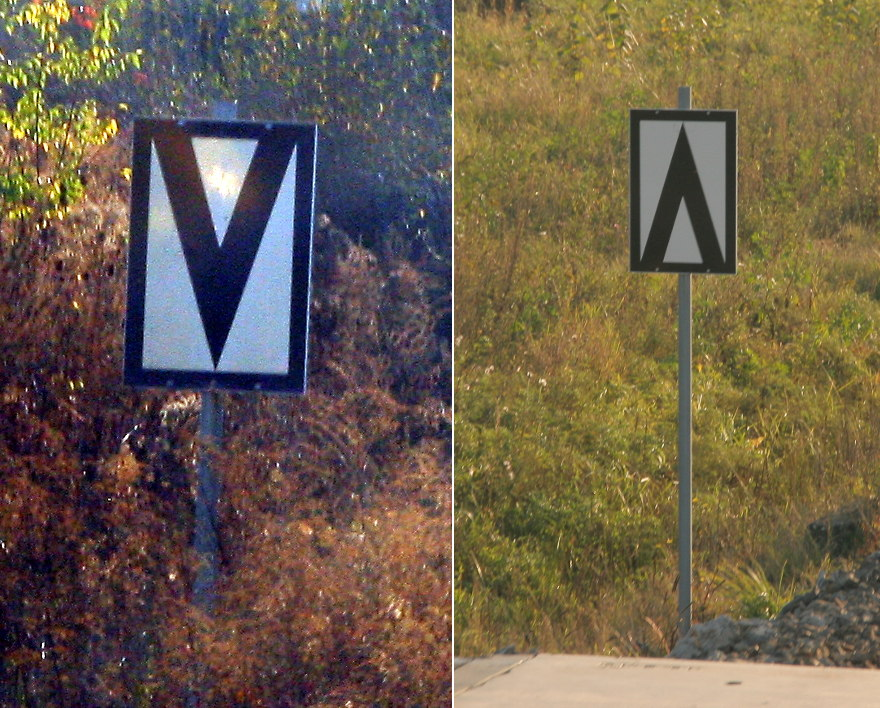
\includegraphics[width=6cm]{skryptkierownik-img/wskazniki-w9.jpg}
	\caption{Wskaźniki W9 początku i końca ograniczenia}
\end{marginfigure}
Wskaźnik W9 {\textquotedbl}Wskaźnik odcinka ograniczonej prędkości{\textquotedbl} oznacza początek lub koniec odcinka, przez który należy przejeżdżać z ograniczoną prędkością. Prostokątna biała tablica z czarnym obramowaniem, a na niej z jednej strony czarny kąt, zwrócony wierzchołkiem ku dołowi, z drugiej zaś - zwrócony wierzchołkiem ku górze (kąt oparty jest na krótszym boku prostokąta, a wierzchołek dotyka przeciwległego boku).

Wskaźnik W 9 należy stosować łącznie ze wskaźnikiem W 8 jeżeli ostrzeżenie jest ujęte w wykazie ostrzeżeń stałych. 

\subsection{W14 - wskaźniki odcinka ograniczonej prędkości}

Prostokątna pomarańczowa tablica z czarnym obramowaniem, a na niej z jednej strony czarny kąt, zwrócony wierzchołkiem ku dołowi, z drugiej zaś - zwrócony wierzchołkiem ku górze (kąt oparty jest na krótszym boku prostokąta, a wierzchołek dotyka przeciwległego boku). Wskaźnik W14 należy stosować łącznie z sygnałem D6 - tarcza “Zwolnić bieg”, stosowany jest do wskazania odcinka o ograniczonej prędkości wskazanego w ostrzeżeniach doraźnych. 

\subsection{W11 - wskaźniki uprzedzające}

Wskaźniki W11a i W11b w zależności od miejsca usytuowania wskaźnika oznaczają, że za wskaźnikiem znajduje się:
	\begin{marginfigure}
	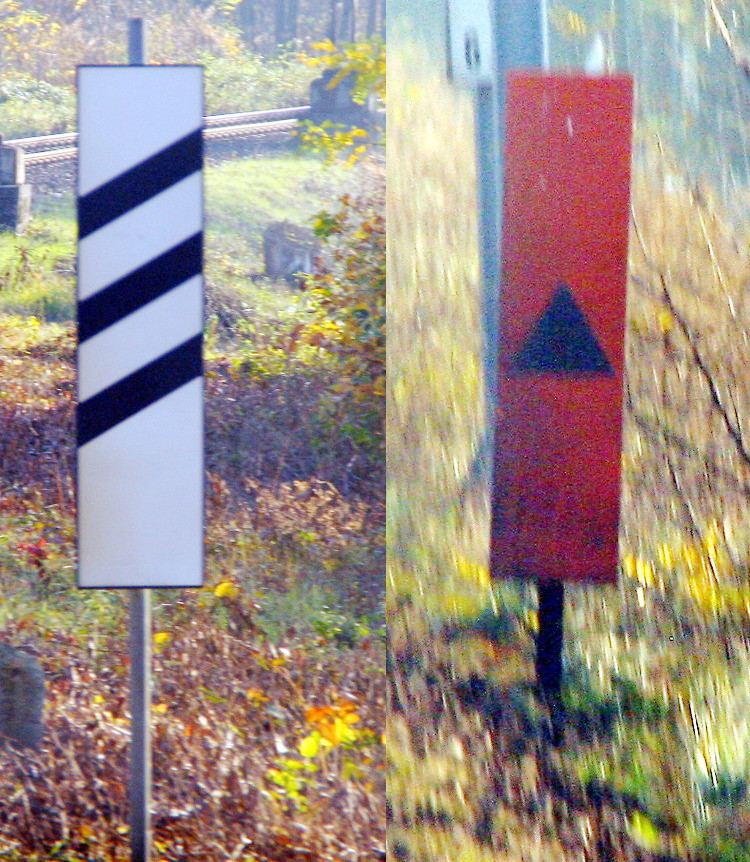
\includegraphics[width=5cm]{skryptkierownik-img/wskazniki-w11.jpg}
	\caption{Wskaźnik W11a (dla odległości 300m od sygnalizatora, z lewej), wskaźnik W11p (z prawej)} 
\end{marginfigure}
a) tarcza ostrzegawcza semafora wjazdowego lub odstępowego albo semafor, którego obrazy sygnałowe mogą nie być widoczne w sposób ciągły z wymaganej odległości (wskaźnik W11a). Wskaźnik ustawia się w co 100m

b) tarcza ostrzegawcza semafora wjazdowego posterunku ruchu, na którym rozpoczyna się odcinek zelektryfikowany (wskaźnik W11b)

c) tarcza ostrzegawcza przejazdowa (wskaźnik W11p). Wskaźnik ustawia się w odległości 200m, a jeśli obrazy sygnałowe mogą nie być widoczne w sposób ciągły z wymaganej odległości, również w odległości 400m.

\subsection{W17 - wskaźnik ukresu}

Wskaźnik W 17 oznacza miejsce przy zbiegających się torach, do którego wolno tor zająć taborem kolejowym. Miejsce usytuowania wskaźnika wyznacza się z uwzględnieniem obowiązującej skrajni i warunków lokalnych, w szczególności przechyłki lub poszerzenia na łuku.

	\begin{marginfigure}
		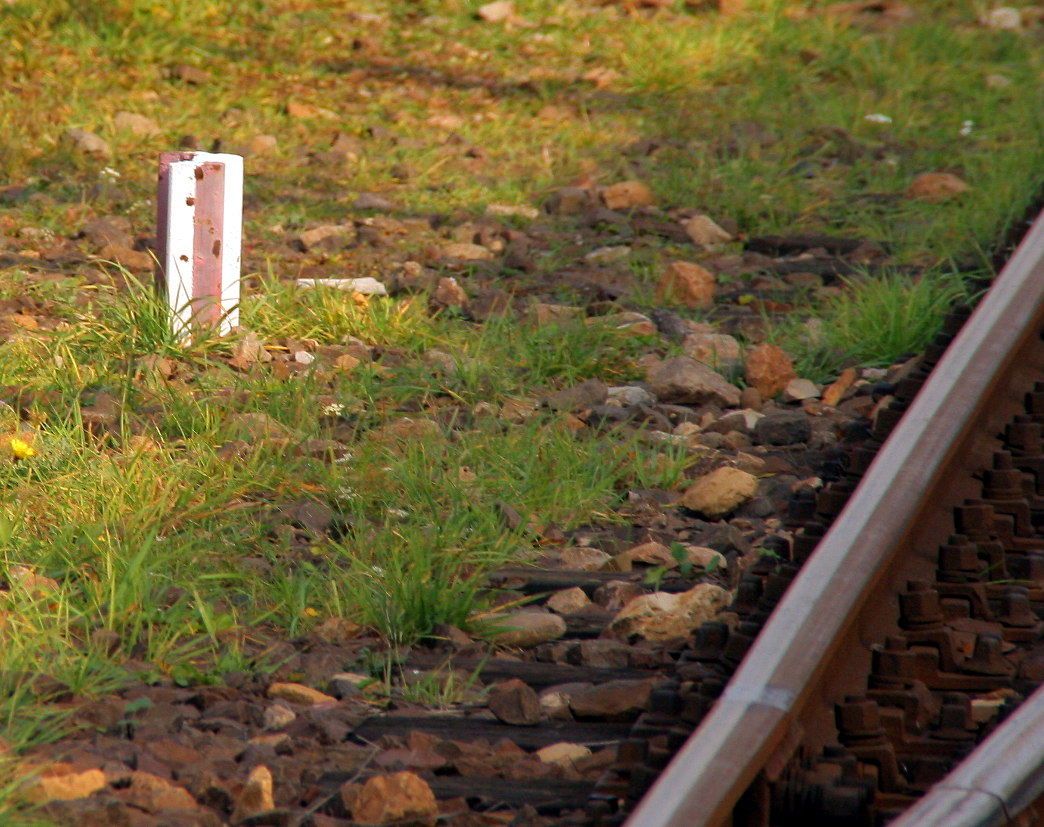
\includegraphics[width=4cm]{skryptkierownik-img/skryptkierownik-img016.jpg}
		\caption{Wskaźnik W17}
	\end{marginfigure}


\subsection{W18 - wskaźnik samoczynnej blokady liniowej}

	\begin{marginfigure}
	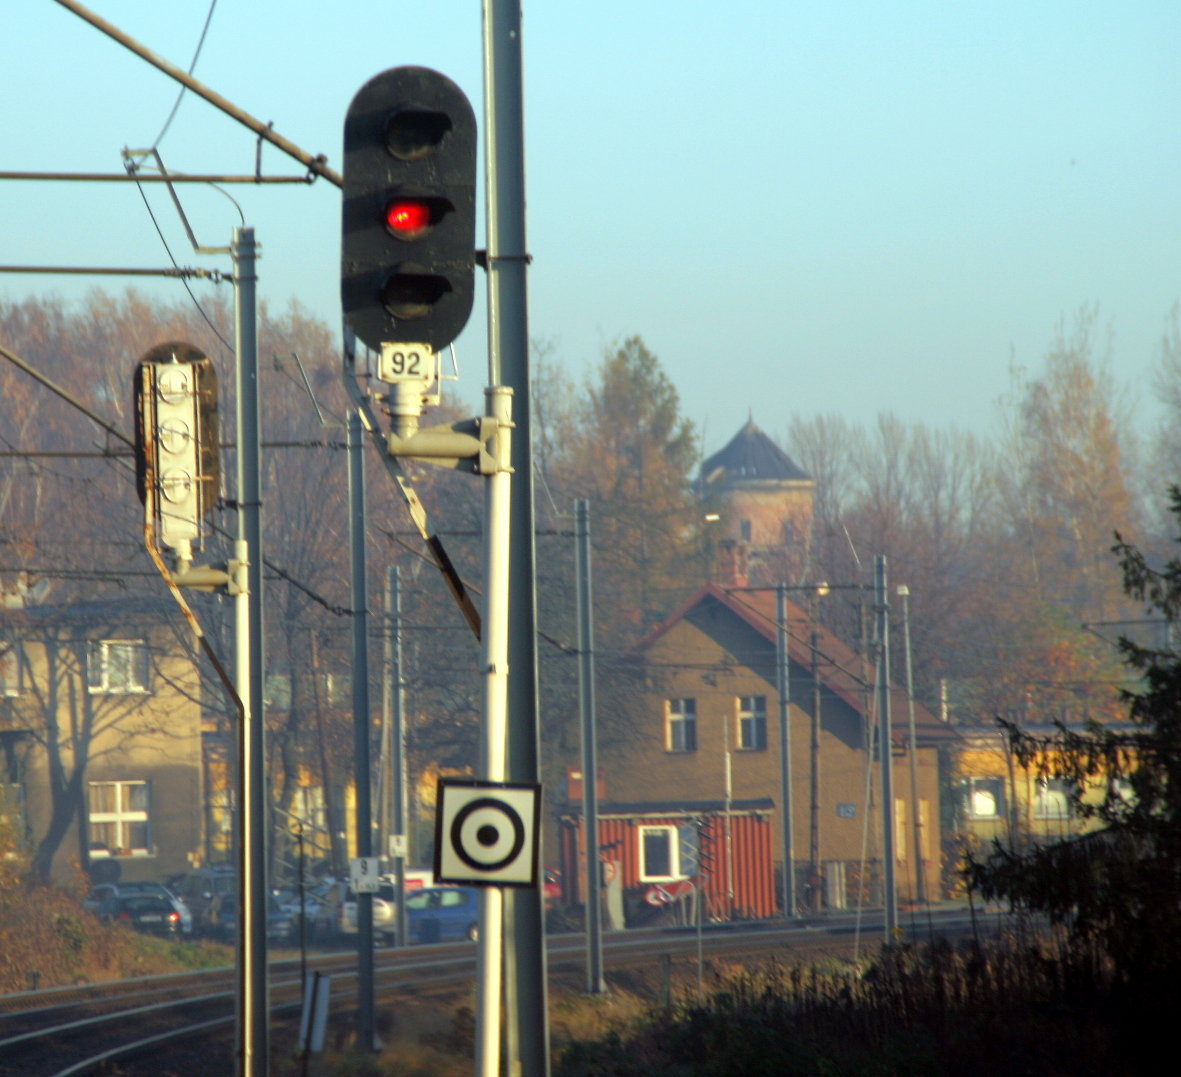
\includegraphics[width=5cm]{skryptkierownik-img/skryptkierownik-img017.jpg}
	\caption{Wskaźnik W18 na maszcie semafora SBL, LK 139, szlak Ligota- Mąkołowiec}
\end{marginfigure}
Wskaźnik W 18 {\textquotedbl}Wskaźnik samoczynnej blokady liniowej{\textquotedbl} oznacza miejsce ustawienia ostatniego semafora odstępowego samoczynnej blokady liniowej na szlaku przed semaforem wjazdowym. Kwadratowa biała tablica z czarnym obramowaniem, a na niej czarny pierścień z czarnym kołem w środku. Wskaźnik W 18 umieszcza się na maszcie ostatniego semafora odstępowego samoczynnej blokady liniowej w celu poinformowania drużyny pociągowej, że zbliża się do semafora wjazdowego posterunku ruchu, w przypadku gdy ostatni samoczynny semafor odstępowy jest ciemny lub
unieważniony, wskaźnik W 18 nakazuje maszyniście jazdę z taką prędkością, aby mógł on zatrzymać pociąg przed ewentualną przeszkodą, semaforem wjazdowym wskazującym sygnał {\textquotedbl}Stój{\textquotedbl} lub zmniejszyć prędkość stosownie do wskazań semafora wjazdowego.

\subsection{W19 - wskaźnik uprzedzający o braku drogi hamowania + W20 - wskaźnik braku drogi hamowania}

Wskaźnik W 19 {\textquotedbl}Wskaźnik uprzedzający o braku drogi hamowania{\textquotedbl} oznacza, że odległość między dwoma następnymi semaforami lub między następną tarczą ostrzegawczą semaforową a semaforem jest mniejsza od obowiązującej na danej linii kolejowej długości drogi hamowania 

Biała strzała, zwrócona ostrzem ku dołowi, na czarnym tle. Wskaźnik W19 informuje drużynę pociągową o tym, że za następnym semaforem lub tarczą ostrzegawczą semaforową pociąg wjedzie na odstęp o długości mniejszej od obowiązującej na danej linii kolejowej drogi hamowania i wymaga od maszynisty zachowania szczególnej ostrożności w regulowaniu
prędkości jazdy pociągu, wskaźnik W19 umieszcza się na maszcie semafora lub tarczy ostrzegawczej semaforowej bezpośrednio poprzedzających ten semafor lub tarczę ostrzegawczą semaforową, za którymi występuje skrócony odstęp. 

Wskaźnik W20 {\textquotedbl}Wskaźnik braku drogi hamowania{\textquotedbl} oznacza, że odległość między tarczą ostrzegawczą semaforową lub semaforem, na których jest umieszczony wskaźnik, a następnym semaforem jest mniejsza od obowiązującej na danej linii kolejowej długości drogi hamowania. 

Dwie równoległe białe strzały, zwrócone ostrzem ku dołowi, na czarnym tle. Wskaźnik W20 informuje drużynę pociągową o
tym, że pociąg wjeżdża na odstęp o długości mniejszej od obowiązującej na danej linii kolejowej drogi hamowania i
wymaga od maszynisty zachowania szczególnej ostrożności w regulowaniu prędkości jazdy pociągu, umieszcza się go na
maszcie tarczy ostrzegawczej semaforowej lub semafora na początku skróconego odstępu, patrząc w kierunku jazdy pociągu,
wskaźnik W20 powinien być poprzedzony wskaźnikiem W19.

\subsection{W21 - wskaźniki zmiany prędkości}

Wskaźnik W21 umieszczony na maszcie semafora oznacza, że jazda po zwrotnicach w kierunku zwrotnym może odbywać się z prędkością określoną przez ten  wskaźnik większą niż 40 km/h, na wskaźniku matowo-biała liczba na czarnym tle wyświetla się jednocześnie z ukazaniem się na semaforze sygnału zezwalającego na jazdę ze zmniejszoną prędkością.

\subsection{W23 - wskaźnik odcinka izolowanego}

Wskaźnik W 23 {\textquotedbl}Wskaźnik odcinka izolowanego{\textquotedbl} początek odcinka torowego lub zwrotnicowego
wyposażonego w urządzenie kontroli niezajętości torów i rozjazdów, oznacza miejsce, przed którym przetaczany tabor
kolejowy powinien się zatrzymać, aby umożliwić przestawienie rozjazdu.

\subsection{W24 - wskaźnik kierunku przeciwnego}

	\begin{marginfigure}
	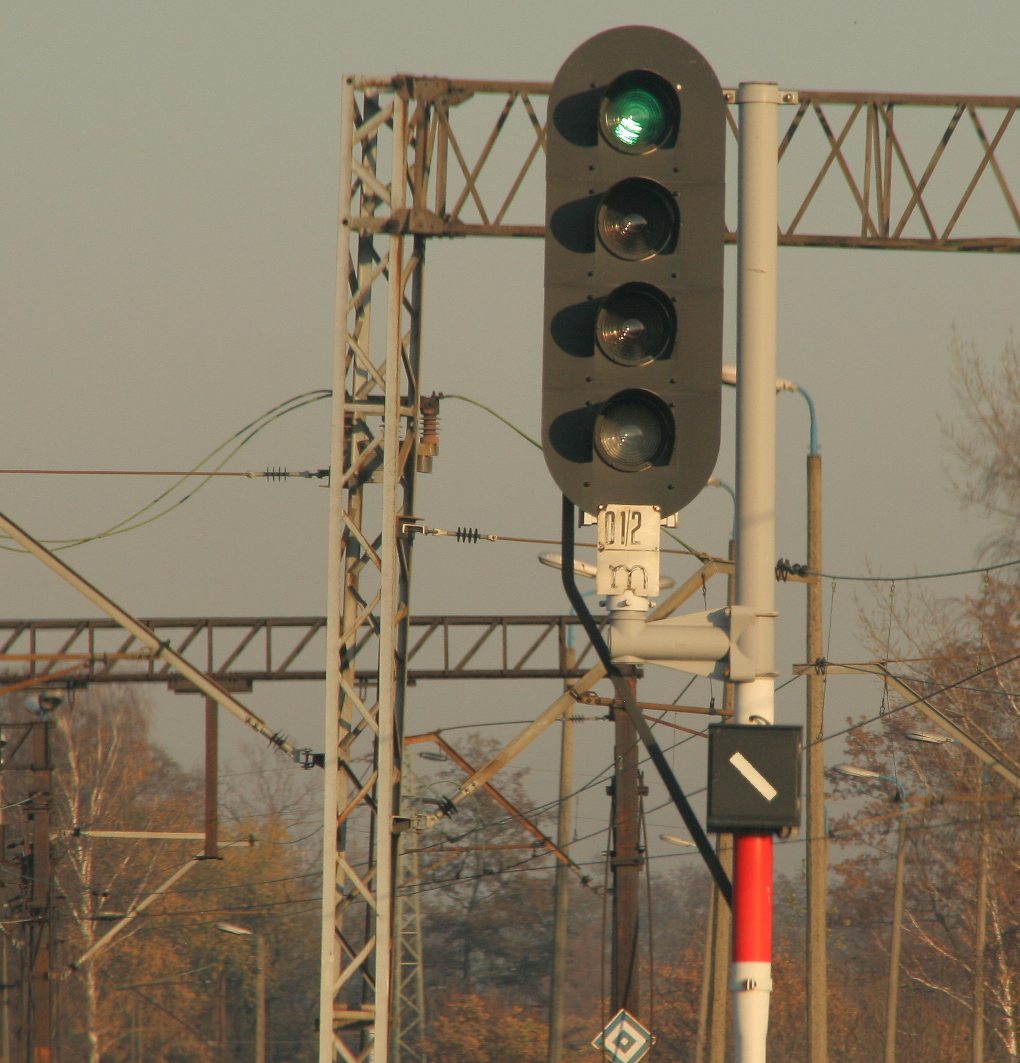
\includegraphics[width=4cm]{skryptkierownik-img/skryptkierownik-img018.jpg}
	\caption{Semafor wyjazdowy ze wskaźnikiem W24}
\end{marginfigure}
Wskaźnik W 24 {\textquotedbl}Wskaźnik kierunku przeciwnego{\textquotedbl} oznacza wyjazd na tor szlaku dwutorowego w kierunku przeciwnym do zasadniczego, matowobiała kresa na kwadratowej czarnej tablicy wznosząca się do góry z prawa na lewo na słupie semafora. Obraz na wskaźniku pokazuje się jednoczesnie z wyświetleniem na semaforze sygnału zezwalającego na jazdę lub “Sz”. 

\subsection{W25 - wskaźnik ogrzewania}

Wskaźnik W25 oznacza stanowisko elektrycznego ogrzewania wagonów i rozpoczęcia ogrzewania. Wskaźnik świetlny - jedna lub dwie prostokątne latarnie umieszczone na wspólnym maszcie; na każdej latarni, w kolorze czerwonym, numer toru ze strzałką zwróconą w kierunku toru, do którego się ta latarnia odnosi, oraz strzała w kształcie błyskawicy zwrócona ostrzem ku dołowi, wskaźnik W25 ustawia się na międzytorzu w miejscu stanowiska elektrycznego ogrzewania wagonów na torach postojowych; przeznaczony jest on do uprzedzenia o konieczności zachowania ostrożności w czasie ogrzewania składów, z uwagi na wysokie napięcie, wyświetla się z chwilą rozpoczęcia ogrzewania, w czasie trwania ogrzewania wagonów zabrania się zbliżania i dojeżdżania do nich.

\subsection{W2, W26, W26b - wskaźniki kierunku jazdy pociągu}

\begin{enumerate}
\item \textbf{Wskaźnik W 2 {\textquotedbl}Wskaźnik kierunku jazdy{\textquotedbl} oznacza kierunek wyjazdu pociągu. Wskaźnik świetlny z matowobiałą literą na czarnym tle, stanowiącą skrót nazwy stacji końcowej lub najbliższej węzłowej danej linii kolejowej bądź innego wyróżnionego punktu docelowego dla wyjazdu pociągu.
\item 
Wskaźniki W 26a i W 26b {\textquotedbl}Wskaźniki kierunku jazdy{\textquotedbl} oznaczają przejazd z grupy torów dalekobieżnych na grupę torów podmiejskich (wskaźnik W 26a) lub przejazd z grupy torów podmiejskich na grupę torów dalekobieżnych (wskaźnik W 26b)} 
\item Wskaźnik świetlny z matowobiałą literą na czarnym tle, stanowiącą skrót nazwy grupy torów, na którą przejeżdża pociąg (wskaźnik W 26a - zawsze litera {\textquotedbl}P{\textquotedbl}, wskaźnik W 26b - zawsze litera
{\textquotedbl}D{\textquotedbl})
\item Wskaźniki W 26a i W 26b umieszcza się na semaforze ustawionym przed przejściem zwrotnicowym służącym do przejazdu z jednej grupy torów na drugą; wskaźnik jest wyświetlany tylko wtedy, kiedy semafor wskazuje sygnał zezwalający na jazdę w kierunku, który został wyróżniony tym wskaźnikiem; wskaźniki W 26a i W 26b wyświetlają się również, gdy na semaforze ukaże się sygnał zastępczy.
\end{enumerate}

\subsection{W27a - wskaźnik zmiany prędkości}

Wskaźnik W 27 ustawia się w miejscu zmiany największej dozwolonej prędkości drogowej na szlaku jednotorowym po prawej stronie toru, patrząc w kierunku wzrostu kilometrażu linii kolejowej (wskaźnik dwustronny, stosownie do prędkości dozwolonej za tym wskaźnikiem, patrząc w kierunku jazdy pociągu).

\subsection{W28 - wskaźnik kanału radiowego}
Okrągła czarna tablica, a na niej żółte oznaczenie literowo-cyfrowe. Oznacza miejsce zmiany i obowiązujący od tego miejsca numer kanału radiołączności pociągowej. Ustawia się go 30-70m za ostatnim rozjazdem, patrząc w kierunku szlaku z radiołącznością pociągową.
	\begin{marginfigure}
		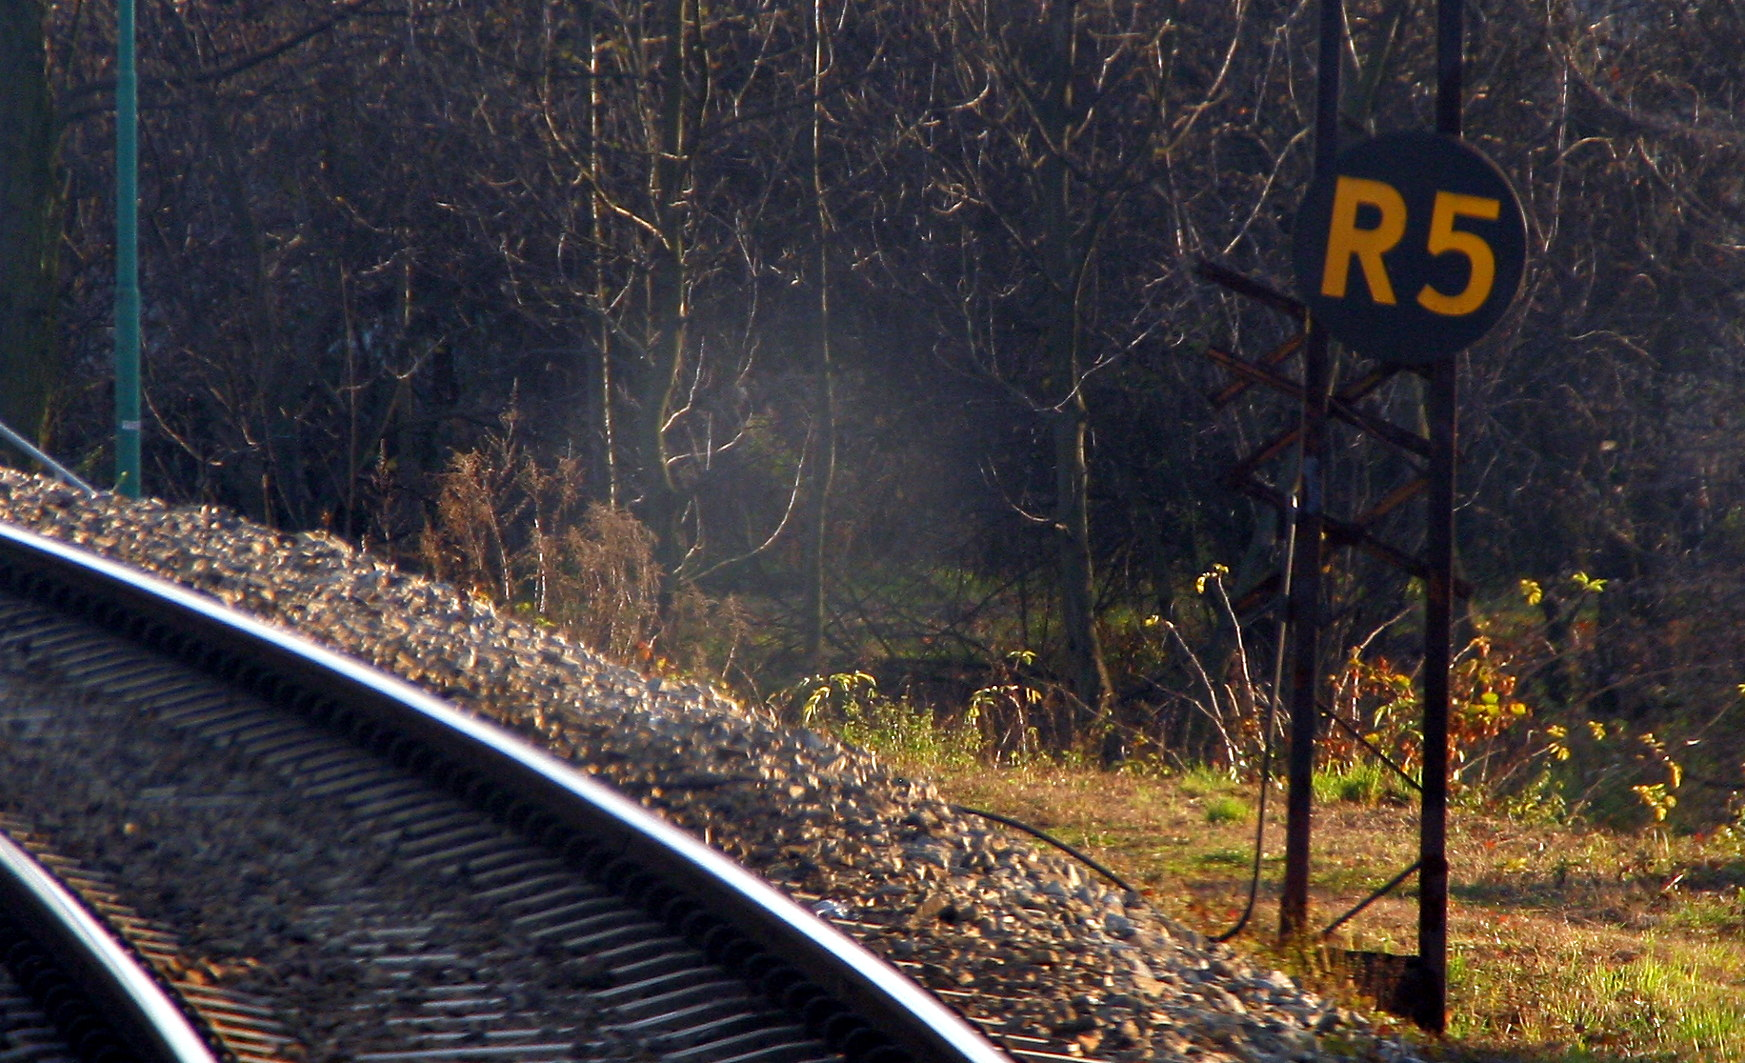
\includegraphics[width=7cm]{skryptkierownik-img/skryptkierownik-img019.jpg}
		\caption{Wskaźnik W28 na szlaku podg Most Wisła - Czechowice-Dziedzice}
		\label{fig:w28}
	\end{marginfigure}

\subsection{W29 - wskaźnik nawiązania łączności}

Oznacza, że należy nawiązać łączność radiową z dyżurnym ruchu odcinkowym

\subsection{W31 - wskaźnik kasowania}

{\textquotedbl}Wskaźnik kasowania{\textquotedbl} oznacza, że sygnalizator, na którym został umieszczony wskaźnik, jest nieczynny, nie został oddany do użytku lub jest unieważniony, a sygnały wyświetlane na nim są nieobowiązujące. Biały ukośny krzyż z czarną obwódką, umieszczony na słupie sygnalizatora, bezpośrednio pod komorami sygnałowymi.

\section{Sygnalizatory}

Maszty semaforów odstępowych samoczynnych na szlakach wyposażonych w blokadę samoczynną są koloru białego.

Maszty semaforów półsamoczynnych pomalowane są w poziome pasy czerwono-białe, z tym że pierwszy pas od dołu masztu jest czerwony. Jeśli latarnia sygnałowa jest zawieszona obok lub nad torem (na bramce) to należy zawiesić listwę pomalowaną
w pasy czerwono-białe.Dla semaforów karzełkowym obowiązuje malowanie w pasy białe i czerwony (środkowy).

Tarcze manewrowe, powtarzacze umieszczone są na maszcie koloru szarego, zaś tarcze przejazdowe na maszcie czarno-białym.

	\begin{figure*}
		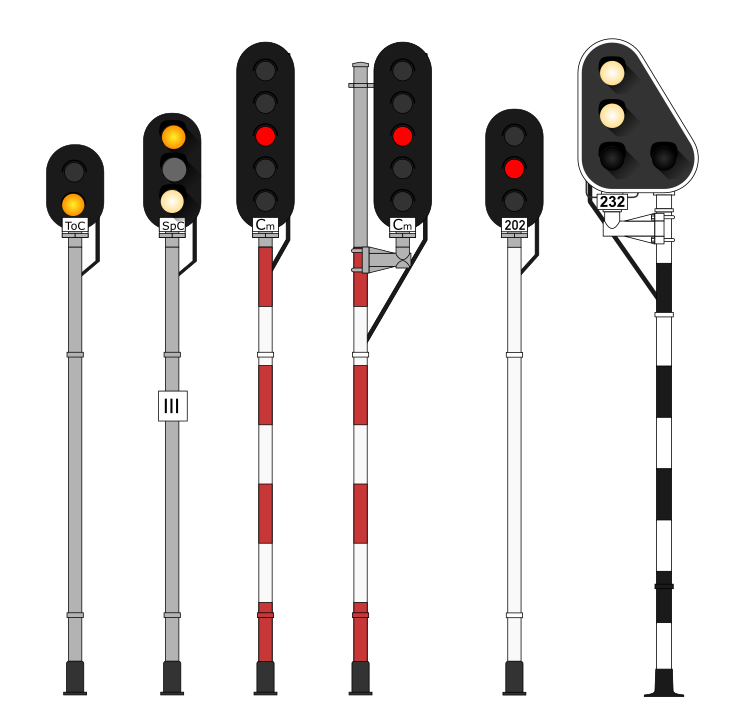
\includegraphics[width=15cm]{skryptkierownik-img/sygnalizatory.png}
		\caption{Sygnalizator semafora półsamoczynnego (podg Most Wisła), Sygnalizator samoczynnej blokady liniowej (szlak Pszczyna - Most Wisła), Tarcza ostrzegawcza semafora st. Cz-Dziedzice Południowe, Tarcza przejazdowa ToP na szlaku Bielsko-Biała Leszczyny - Wilkowice-Bystra}
	\end{figure*}


\section{Sygnały}

\subsection{Tarcze DO i D1}

Tarczę zatrzymania D1 „Stój” ustawia się po prawej stronie toru szlakowego, w odległości 50m przed przeszkodą. W torach stacyjnych tarczę nalezy ustawić w osi toru, 100 m przed przeszkodą. Odległość ta może zostanie skrócona jeśli nie pozwalają warunki miejscowe. W przypadku zamknięcia toru szlakowego pomiędzy posterunkami zapowiadawczymi, nalezy oprocz osygnalizowania przeszkody na miejscu, wystawić tarczę D1 bezpośrednio za ostatnim rozjadem w stacji w kierunku szlaku. Maszyny torowe i pojazdy specjalistyczne osłania się ustawiając tarczę D1 w odległości 3m od maszyny w osi toru.
\ \ Tarczę DO należy ustawić w odległości drogi hamowania zwiększonej o 200m od tarczy D1. W stacjach tarczy DO nie stosuje się.
	\begin{marginfigure}
	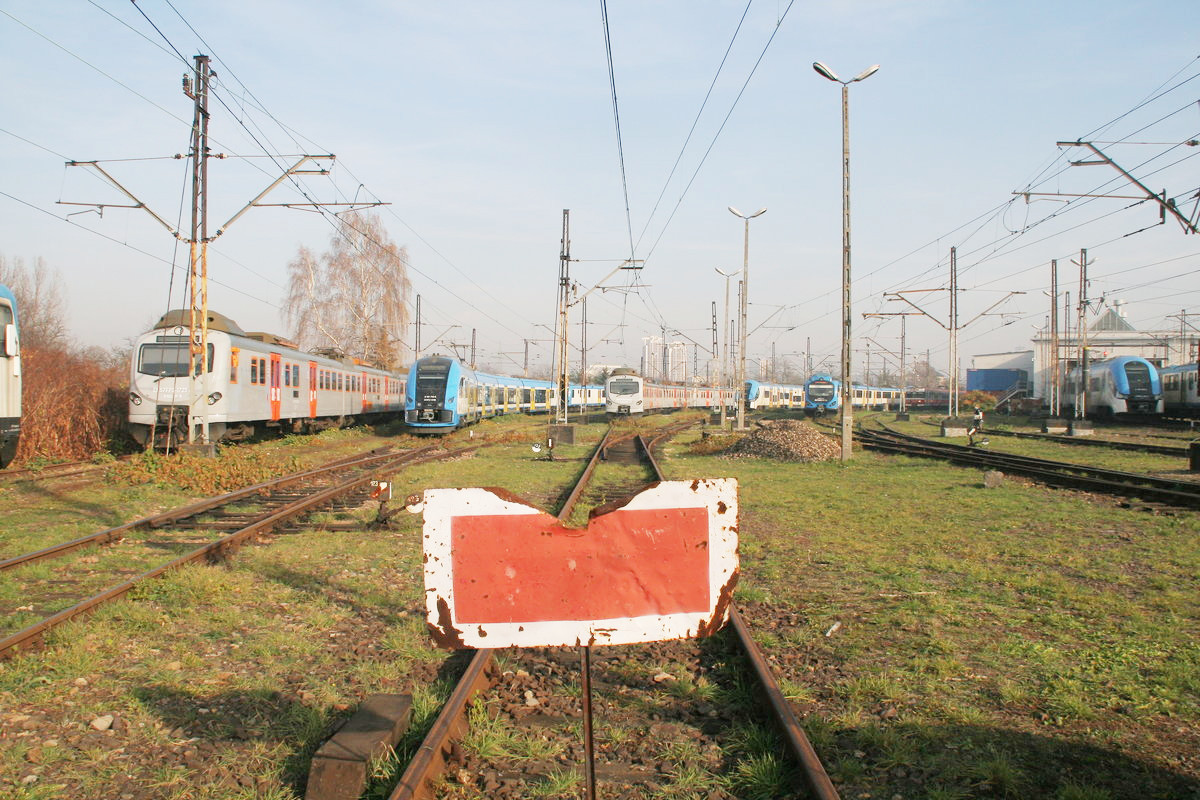
\includegraphics[width=7cm]{skryptkierownik-img/skryptkierownik-img023.jpg}
	\caption{Tarcza D1 w osi toru}
\end{marginfigure}

\chapter{Przygotowanie drogi przebiegu dla jazd pociągowych i manewrowych}


Droga przebiegu to droga jazdy pomiędzy dwoma kolejnymi sygnalizatorami uzupełniona w miarę potrzeby drogą ochronną oraz urządzeniami ochronnymi. W pierwszej kolejności układa się drogę rozjazdową, poprzez właściwe ustawienie zwrotnic i wykolejnic w terenie, właściwe ustawienie urządzeń zależnościowych takich jak zamki zwrotnicowe i wykolejnicowe, obsługa aparatu blokowego, etc. Następnym krokiem jest zamknięcie (zaryglowanie) a potem utwierdzenie drogi przebiegu, to jest zablokowanie możliwości zmiany ułożenia rozjazdów i wskazań sygnalizatora, do czasu przejechania pociągu poza daną drogę przebiegu.

Przygotowanie drogi przebiegu polega na usunięciu z drogi przebiegu pociągu wszelkiego taboru, przerwaniu manewrów, nastawieniu rozjazdów, oraz zabezpieczeniu przed przypadkowym przełożeniem. Kolejnym etapem jest powiadomienie posterunków dróżników przejazdowych. Ostatnim krokiem jest wyświetlenie sygnałów zezwalających na jazdę manewrową lub pociągową.

\begin{itemize}
	\item Przebieg – przygotowana droga przebiegu z realizacją wszystkich wymaganych uzależnień wraz z podaniem sygnału zezwalającego na jazdę taboru.
	\item Przebieg manewrowy – przebieg dla manewrującego taboru na stacji.
	\item Przebieg pociągowy – przebieg dla pociągu w granicach stacji.
	\item Przebieg niezorganizowany – przebieg, którego droga przebiegu nie jest utwierdzona ani zamknięta.
	\item Przebieg sprzeczny – przebieg, który ze względu bezpieczeństwa nie może być realizowany jednocześnie z innym. 
\end{itemize}

\chapter{Prowadzenie dokumentacji techniczno-ruchowej}

Dyżurny ruchu prowadzi dokumentację techniczno-ruchową w stacji i na przyległych szlakach. 
Podstawowym dokumentem jest dziennik ruchu \textbf{R-146}. Wprowadza się do niego informację o numerze i kierunku (parzysty/nieparzysty), godzinach odjazdu, przyjazdu do posterunku, drodze wolnej. Również uwagi o przejeździe pociągu z TWR, braku sygnałów końca pociągu. Dodatkowo znajdują się tu również informacje o powiadamianiu dróżników przejazdowych. W dzienniku tym umieszcza się również informację o wprowadzeniu ruchu jednotorowego dwukierunkowego.

Książka przebiegów \textbf{R-142} służy do odnotowania poleceń przygotowania wjazdów/wyjazdów dla nastawni wykonawczej. Znajdują się tam informacje o numerze pociągu, torze stacyjnym, oraz godzinach polecenia przygotowania drogi, wyświetlenia semafora.

Dziennik telefoniczny \textbf{R-138} w którym odnotowuje się np. informacje o zgłoszeniu gotowości pociągu, skomunikowaniach, zamknięciu lub otwarciu toru szlakowego. 

Książka urządzeń SRK \textbf{E-1758} w której odnotowuje się wszystkie zdarzenia związane z zerwaniem plomb na urządzeniach, oraz wyświetleniem sygnału zastępczego (które jest rejestrowane licznikiem). 

Dziennik oględzin rozjazdów \textbf{D-831} w którym odnotowywane są wykonywane przez zwrotniczych lub nastawniczych oględziny i prace w rozjazdach, a także wszelkie uwagi co do ich stanu.

Książka ostrzeżeń doraźnych \textbf{R-189} prowadzona jest dla szlaku(linii kolejowej). Obecnie prowadzona jest w formie elektronicznej przez dyżurnego ruchu inspekcyjnego.

Kontrolka zajętości torów \textbf{R-292} opisuje stan zajętości torów stacyjnych (wjazdowych) w momencie przyjęcia/zdania dyżuru.

Pozostałe elementy dokumentacji techniczno-ruchowej to rozkazy pisemne ''O'', ''S'',''N'',''Nrob''

\chapter{Rozkazy pisemne i ostrzeżenia dla drużyn pociągowych}

\textbf{Rozkaz pisemny ''O''} - wydaje się w celu przekazania poleceń i informacji dotyczących ostrożnej jazdy, ostrożnej
jazdy z poleceniem zmniejszenia prędkości (np. uszkodzenie SSP, stan SRK, stan drogi kolejowej), Rozkaz pisemny “O”
musi być odebrany przez drużynę pociągową w stacji oznaczonej w wewnętrznym rozkładzie jazdy symbolem “\textbf{R307}”.
Rozkaz pisemny “O” może być wydany na nieustalonym druku (nawet na czystej kartce).  \begin{tcolorbox}[colback=green!5!white,colframe=green!45!black,width=10cm,title=Rozkaz pisemny ''O'']
	W komputerowym wydruku rozkazu pisemnego ''O'' mogą być przekazywane elementy rozkazów ''S'', ''Nrob'' stanowiące \textbf{informacje}
\end{tcolorbox}
 \marginnote{Ir-1 Rozdział 8, par. 60, ust. 10)}. 

\textbf{Rozkaz pisemny ''S''} - wydaje się w celu przekazania zezwoleń, poleceń i informacji. Przykładowo wydaje się go w
następujących sytuacjach:

	\begin{marginfigure}
		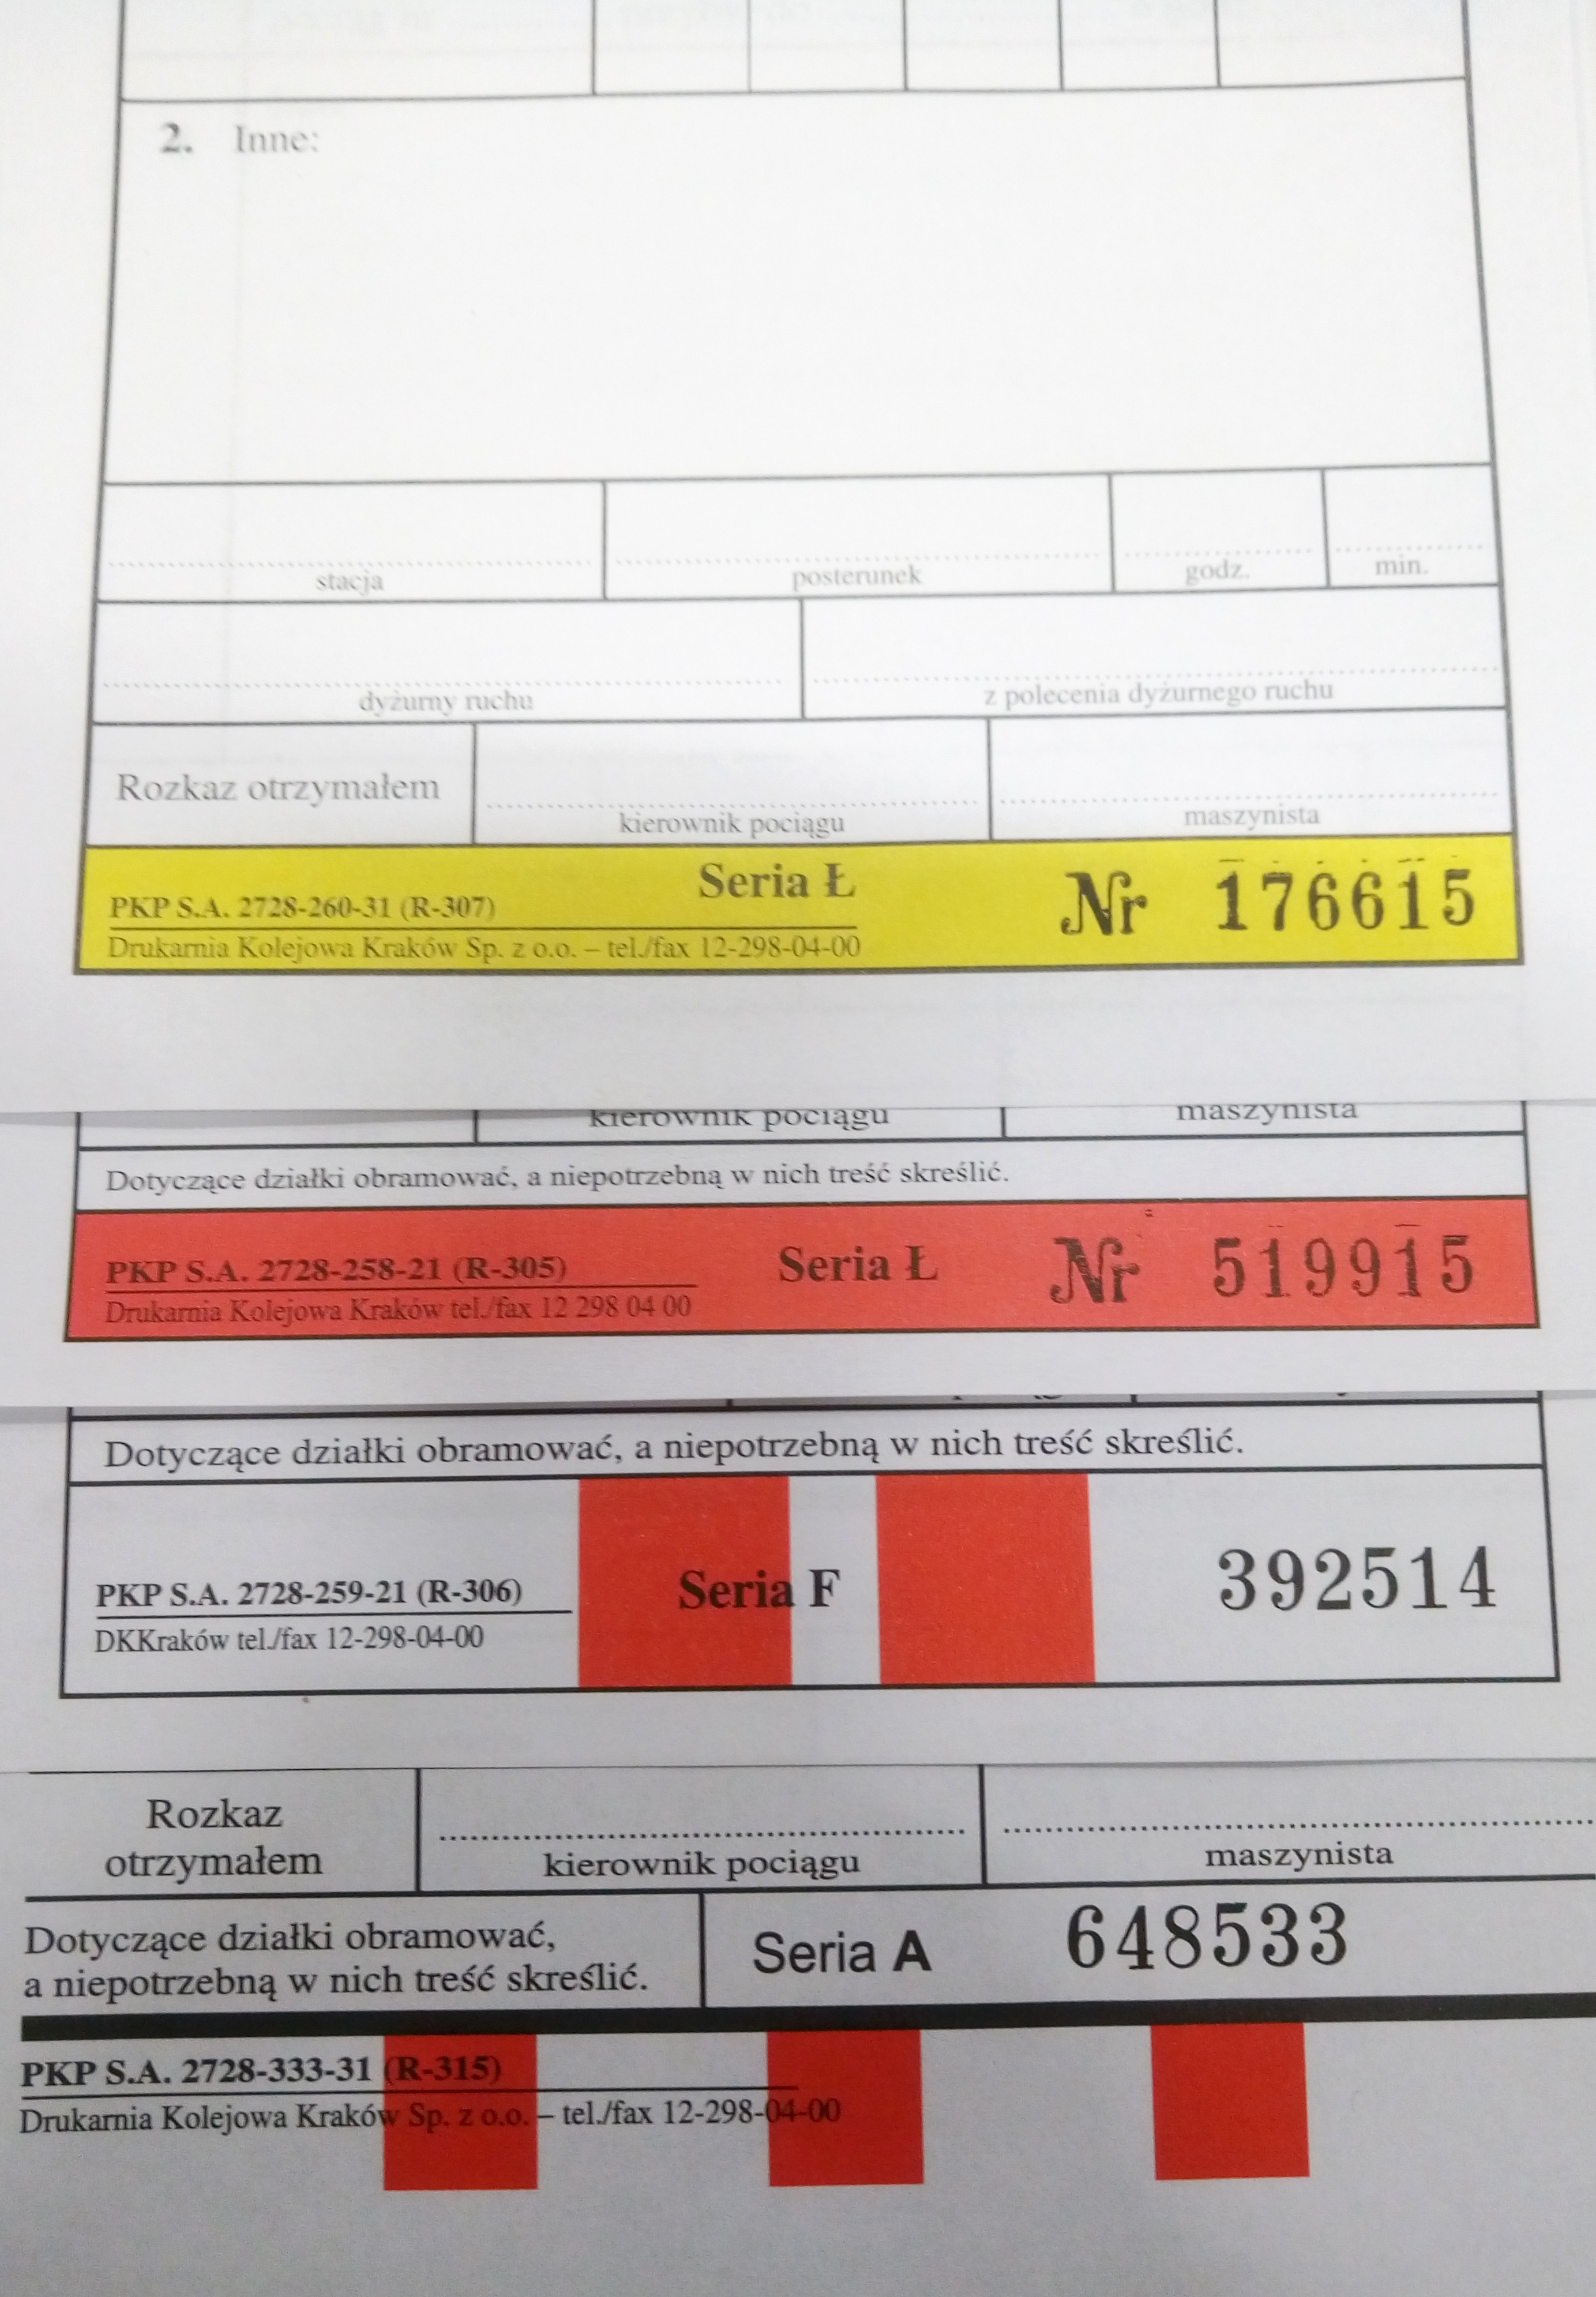
\includegraphics[width=8cm]{skryptkierownik-img/rozkazy-pisemne.jpg}
		\caption{Druki rozkazów pisemnych: od góry ''O'', ''S'', ''N'', ''Nrob''}
	\end{marginfigure}
\begin{itemize}
\item zezwolenie przejechania obok semafora wyjazdowego, wjazdowego, drogowskazowego, wskazującego sygnał “Stój”, sygnał
wątpliwy, białe światło lub nieoświetlonego, jeśli nie można wyświetlić sygnału zastępczego “Sz”.
\item zezwolenie na jazdę manewrową taboru w kierunku szlaku poza ustaloną granicę przetaczania
\item zezwolenie na jazdę w przypadku gdy pojazd trakcyjny znajduje się poza semaforem wskazującym sygnał zezwalający,
którego prowadzący pojazd kolejowy nie widzi.
\item zezwolenie na przejechanie obok tarczy zatrzymania “D1”
\item polecenie jazdy po zamkniętym torze szlakowym i okolicznościach (np. jazda do kilometra i powrót) - w przypadku jazdy na tor zajęty, z przeszkodą, z prędkością do 30 km/h, na tor wolny z prędkością rozkładową.
\item polecenie nie przewidzianego w rozkładzie jazdy zatrzymania pociągu, z określeniem celu i czasu postoju
\item informacja o ustawieniu nowych lub zmianie ustawienia sygnalizatora (przez 14 dni)
\item informacja o jeździe pociągu w innym kierunku niż przewidziany w w.r.j.
\end{itemize}

\textbf{Rozkaz pisemny ''N'' } - wydaje się drużynie pociągowej w celu przekazania zezwoleń, poleceń i informacji o wyjeździe pociągu na tor szlakowy lewy ( w kierunku przeciwnym do zasadniczego), gdy semafor wyjazdowy wskazuje sygnał ''Stój'', o wjeździe pociągu z toru lewego i co będzie sygnałem zezwalającym na wjazd, informację o tym że przejazd pociągu po torze lewym obok posterunków odstępowych może nastąpić po otrzymaniu ręcznego sygnału Rm1 “Do mnie” od dyżurnego, zawsze wtedy gdy ruch prowadzony jest jednotorowo, dwukierunkowo, a tor zasadniczy dla tego kierunku ruchu  jest zamknięty.

W czasie planowych zamknięć torów, w celu wykonania robót, drużynie pociągowej potrzebne zezwolenia, polecenia i informacje mogą być wydawane za pomocą \textbf{rozkazu pisemnego ''Nrob''}. Informacje i zezwolenia dyżurny ruchu wprowadza na podstawie regulaminu tymczasowego, wydawanego na czas robót.

Rozkazy pisemne wystawia dyżurny ruchu dysponujący danego posterunku, zaś techniczną czynność wypisania i doręczenia rozkazu może wykonać inny, upoważniony pracownik (np. zwrotniczy, nastawniczy, etc.), na \textbf{polecenie} dyżurnego ruchu. Jeśli posterunek ruchu jest wyposażony w urządzenia rejestrujące połączenia telefoniczne i radiowe (w rozkładzie przy stacji symbol \textbf{RT}), rozkaz pisemny może być przekazany drogą radiotelefoniczną, w czasie biegu pociągu (wyłącznie przy dwuosobowej obsadzie drużyny trakcyjnej i poniżej 130 km/h).

Numeracja rozkazów pisemnych w bloczku jest w porządku rocznym. Jeśli rozkaz przekazywany jest drogą radiotelefoniczną, to na druku znajdującym się na pojeździe trakcyjnym należy numer rozkazu wpisywać wg podwójnej numeracji - (jako pierwszy numer kolejny na pojeździe, a następnie numer na posterunku ruchu)

\chapter{Wewnętrzny rozkład jazdy}

\section{Elementy rozkładu jazdy}
Rozkład jazdy pociągów to podstawowy element organizacji przewozów kolejowych stanowiący plan pracy kolei, według którego odbywa się ruch wszystkich pociągów po sieci kolejowej lub jej części.  Rozkład jazdy prezentowany jest jako karty rozkładu jazdy. Każda karta rozkładu jazdy, składa się ze strony tytułowej oraz szczegółowego rozkładu jazdy dla pociągu. Aktualnie istnieją dwa dodatki do wewnętrznego rozkładu jazdy:
\begin{tcolorbox}[colback=green!5!white,colframe=green!75!black,width=16cm,title=Dodatki do rozkładu jazdy]
\begin{itemize}
	\item Dodatek 1. do WRJ zawiera Warunki techniczno-ruchowe linii kolejowych zarządzanych przez PLK. Dodatek 1. do WRJ jest
	opracowywany okresowo.
	\item Dodatek 2. do WRJ zawiera wykaz ostrzeżeń stałych oraz prędkości drogowych na torach głównych zasadniczych stacji
	węzłowych. Dodatek 2. do WRJ jest opracowywany okresowo, przy czym po raz pierwszy równocześnie z wejściem w życie rocznego RJ.
\end{itemize}
\end{tcolorbox}
Ostrzeżenia dzielą się na \textbf{stałe} i \textbf{doraźne}. Ostrzeżeniami doraźnymi są ostrzeżenia nie ujęte w wykazie ostrzeżeń stałych. W wykazie ostrzeżeń stałych należy wskazać wszystkie ostrzeżenia, które trwać będą dłużej niż 30 dni.
W wykazie ostrzeżeń stałych umieszczone są odstępstwa od rozkładu jazdy, takie jak ograniczenia prędkości, zachowanie szczególnej ostrożności. Zmiany w WOS wprowadzane są w postaci "poprawek". Mogą one dotyczyć wyłącznie zmniejszenia dolegliwości ograniczenia, np. skreślenia całości ograniczenia, skrócenia kilometrażu objętego ograniczeniem, czy zwiększenia prędkości. Poprawką do WOS nie może być wprowadzone zmniejszenie prędkości. 
Wewnętrzny rozkład jazdy tworzony jest w formie tabeli. \begin{figure*}
	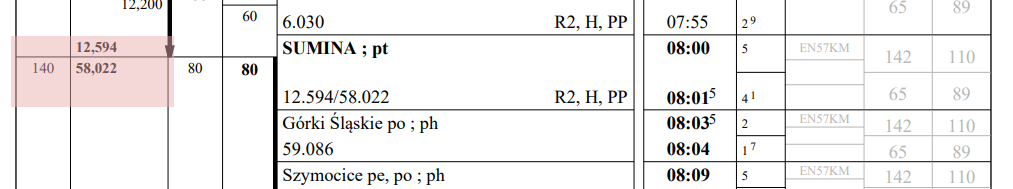
\includegraphics[width=12cm]{skryptkierownik-img/numer-linii.png}
	\caption{Numer linii oraz kilometraż}
\end{figure*} W kolumnie pierwszej znajduje się numer linii zgodnie z wykazem linii PKP PLK. W kolumnie drugiej znajduje się kilometraż początku i końca danego odcinka linii (strona lewa), oraz kilometraż zmiany prędkości rozkładowej (strona prawa). 

\begin{table}
	\begin{tabular}{|c|m{4cm}|c|m{4cm}|}
		\hline 
		m & stacja mijanka & Rd1 & zezwolenie na wyjazd pociągu pasażerskiego - obowiązuje sygnał Rd1 "Nakaz Jazdy" \\ 
		\hline
		skp & posterunek stwierdzania końca pociągu & R1& Numer kanału radiołączności\\ 
		\hline
		po	& przystanek osobowy & H & zainstalowane są urządzenia SHP\\ 
		\hline
		podg	& posterunek odgałeźny &  R307	& posterunek z którego nie można odjechać, bez otrzymania rozkazu pisemnego 'O'\\ 
		\hline
		pt	& postój techniczny & zp & zatrzymanie dla zabrania pracowników (post. ruchu)\\ 
		\hline
		\textbf{Stacja}	& Nazwa stacji & \textbf{STACJA} & Nazwa stacji węzłowej \\ 
		\hline
		W24	& \multicolumn{3}{m{9cm}|}{posterunek na którym zezwoleniem na wyjazd na tor szlakowy lewy jest sygnał zezwalający lub Sz wraz z wyświetlonym wskaźnikiem W24} \\
		\hline
	\end{tabular} 
	\caption{Objaśnienia znaków i skrótów (str. stałe) w.r.j - opisy stacji}
\end{table}
W kolumnie trzeciej znajduje się informacja o prędkości rozkładowej (drogowej) odcinka linii, a także po którym torze został opracowany rozkład.
\begin{figure*}
	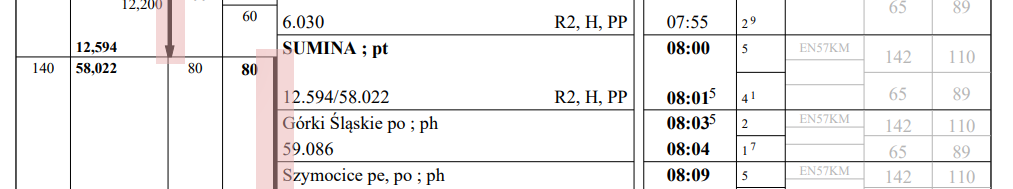
\includegraphics[width=12cm]{skryptkierownik-img/tor-lewy.png}
	\caption{Wskazanie po którym torze opracowano rozkład i prędkości rozkładowe}
\end{figure*}

W kolumnie czwartej znajdują się nazwy posterunków ruchu przez które pociąg ma przejeżdżać, wraz z opisem technicznym (typ postoju, numer kanału radiowego).Opis w polu stacji zawiera również informacje o rodzaju blokady na który nastąpi wyjazd na tor szlakowy. 
\begin{margintable}
	\begin{tabular}{|c|m{4.5cm}|}   
		\hline
		PP	& blokada półsamoczynna przystosowana do jazdy po torze lewym (przeciwnym do zasadniczego) \\ 
		\hline
		S	& blokada samoczynna na szlaku jednotorowym, lub samoczynna jednokierunkowa w kierunku zasadniczym \\ 
		\hline
		SS	& blokada samoczynna przystosowana do jazdy po torze lewym (przeciwnym do zasadniczego) \\ 
		\hline
		SP	& dla kierunku zasadniczego blokada samoczynna, dla toru kierunku przeciwnego półsamoczynna \\ 
		\hline
		PS	& blokada półsamoczynna dla jazdy pociągu w kierunku zasadniczym, blokada samoczynna przystosowana do jazdy po torze lewym (przeciwnym do zasadniczego) \\ 
		\hline
	\end{tabular} 
	\caption{Przystosowanie blokady liniowej do ruchu dwukierunkowego}
\end{margintable}
W kolumnie piątej znajduje się informacja o godzinie przyjazdu i odjazdu dla danego posterunku. Jeśli w polu znajduje się tylko jedna godzina, oznacza to że nie jest przewidywany postój na tym posterunku. W tej samej kolumnie znajduje się również informacja o zmianie numeru pociągu (np. zmiana kierunku jazdy). W pozostałych kolumnach wskazane są informacje o taborze planowym, masie brutto, długości pociągu, prędkości maksymalnej taboru, oraz procencie wymaganym masy hamującej.
\begin{figure*}
	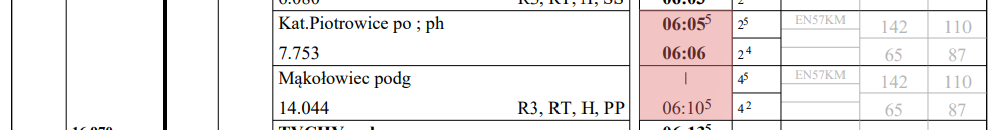
\includegraphics[width=12cm]{skryptkierownik-img/rozklad-odjaz.png}
	\caption{Rozkładowa godzina odjazdu pociągu}
\end{figure*}


\section{Numeracja pociągów}

Pociągi pasa­żerskie krajowe ozna­czane są nume­rami cztero- i pięcio­cyfro­wymi, a pociągi towa­rowe krajowe, utrzymaniowo-naprawcze i niehan­dlowe nume­rami sześcio­cyfro­wymi. Numer pociągu ma być jedno­lity i ma nie zmieniać się na całej trasie pociągu. Numery pociągów międzynaro­dowych usta­lane mają być według odrębnych zasad.

Pierwsza i druga cyfra w numerach cztero-, pięcio- i sześciocyf­rowych określa obszar konstruk­cyjny urucho­mienia i rozwią­zania pociągu. Obszary konstruk­cyjne ozna­czone są nastę­pują­cymi numerami:

1 - Warszawa,\\
2 - Lublin,\\
3 - Kraków,\\
4 - Sosnowiec,\\
5 - Gdańsk,\\
6 - Wrocław,\\
7 - Poznań,\\
8 - Szczecin,\\
9 - rezerwa.\\

Dla pociągów rozpoczyna­jących i kończących bieg wewnątrz jednego obszaru konstrukcyj­nego stoso­wane mogą być następu­jące kombi­nacje dwóch pierwszych cyfr numeru:

11, 10, 19, 91 - Warszawa,\\
22, 20, 29 - Lublin,\\
33, 30, 39, 93 - Kraków,\\
40, 44, 90, 94, 99 - Sosnowiec,\\
55, 50, 59, 95, 96, 97 - Gdańsk,\\
66, 60, 69 - Wrocław,\\
77, 70, 79 - Poznań,\\
88, 80, 89 - Szczecin,\\
92, 98 - rezerwa.\\
Pozostałe cyfry ozna­czają rodzaj pociągu i nada­wane być powinny zgodnie z kolej­nością urucha­miania pociągów w dobie.
\begin{figure}
	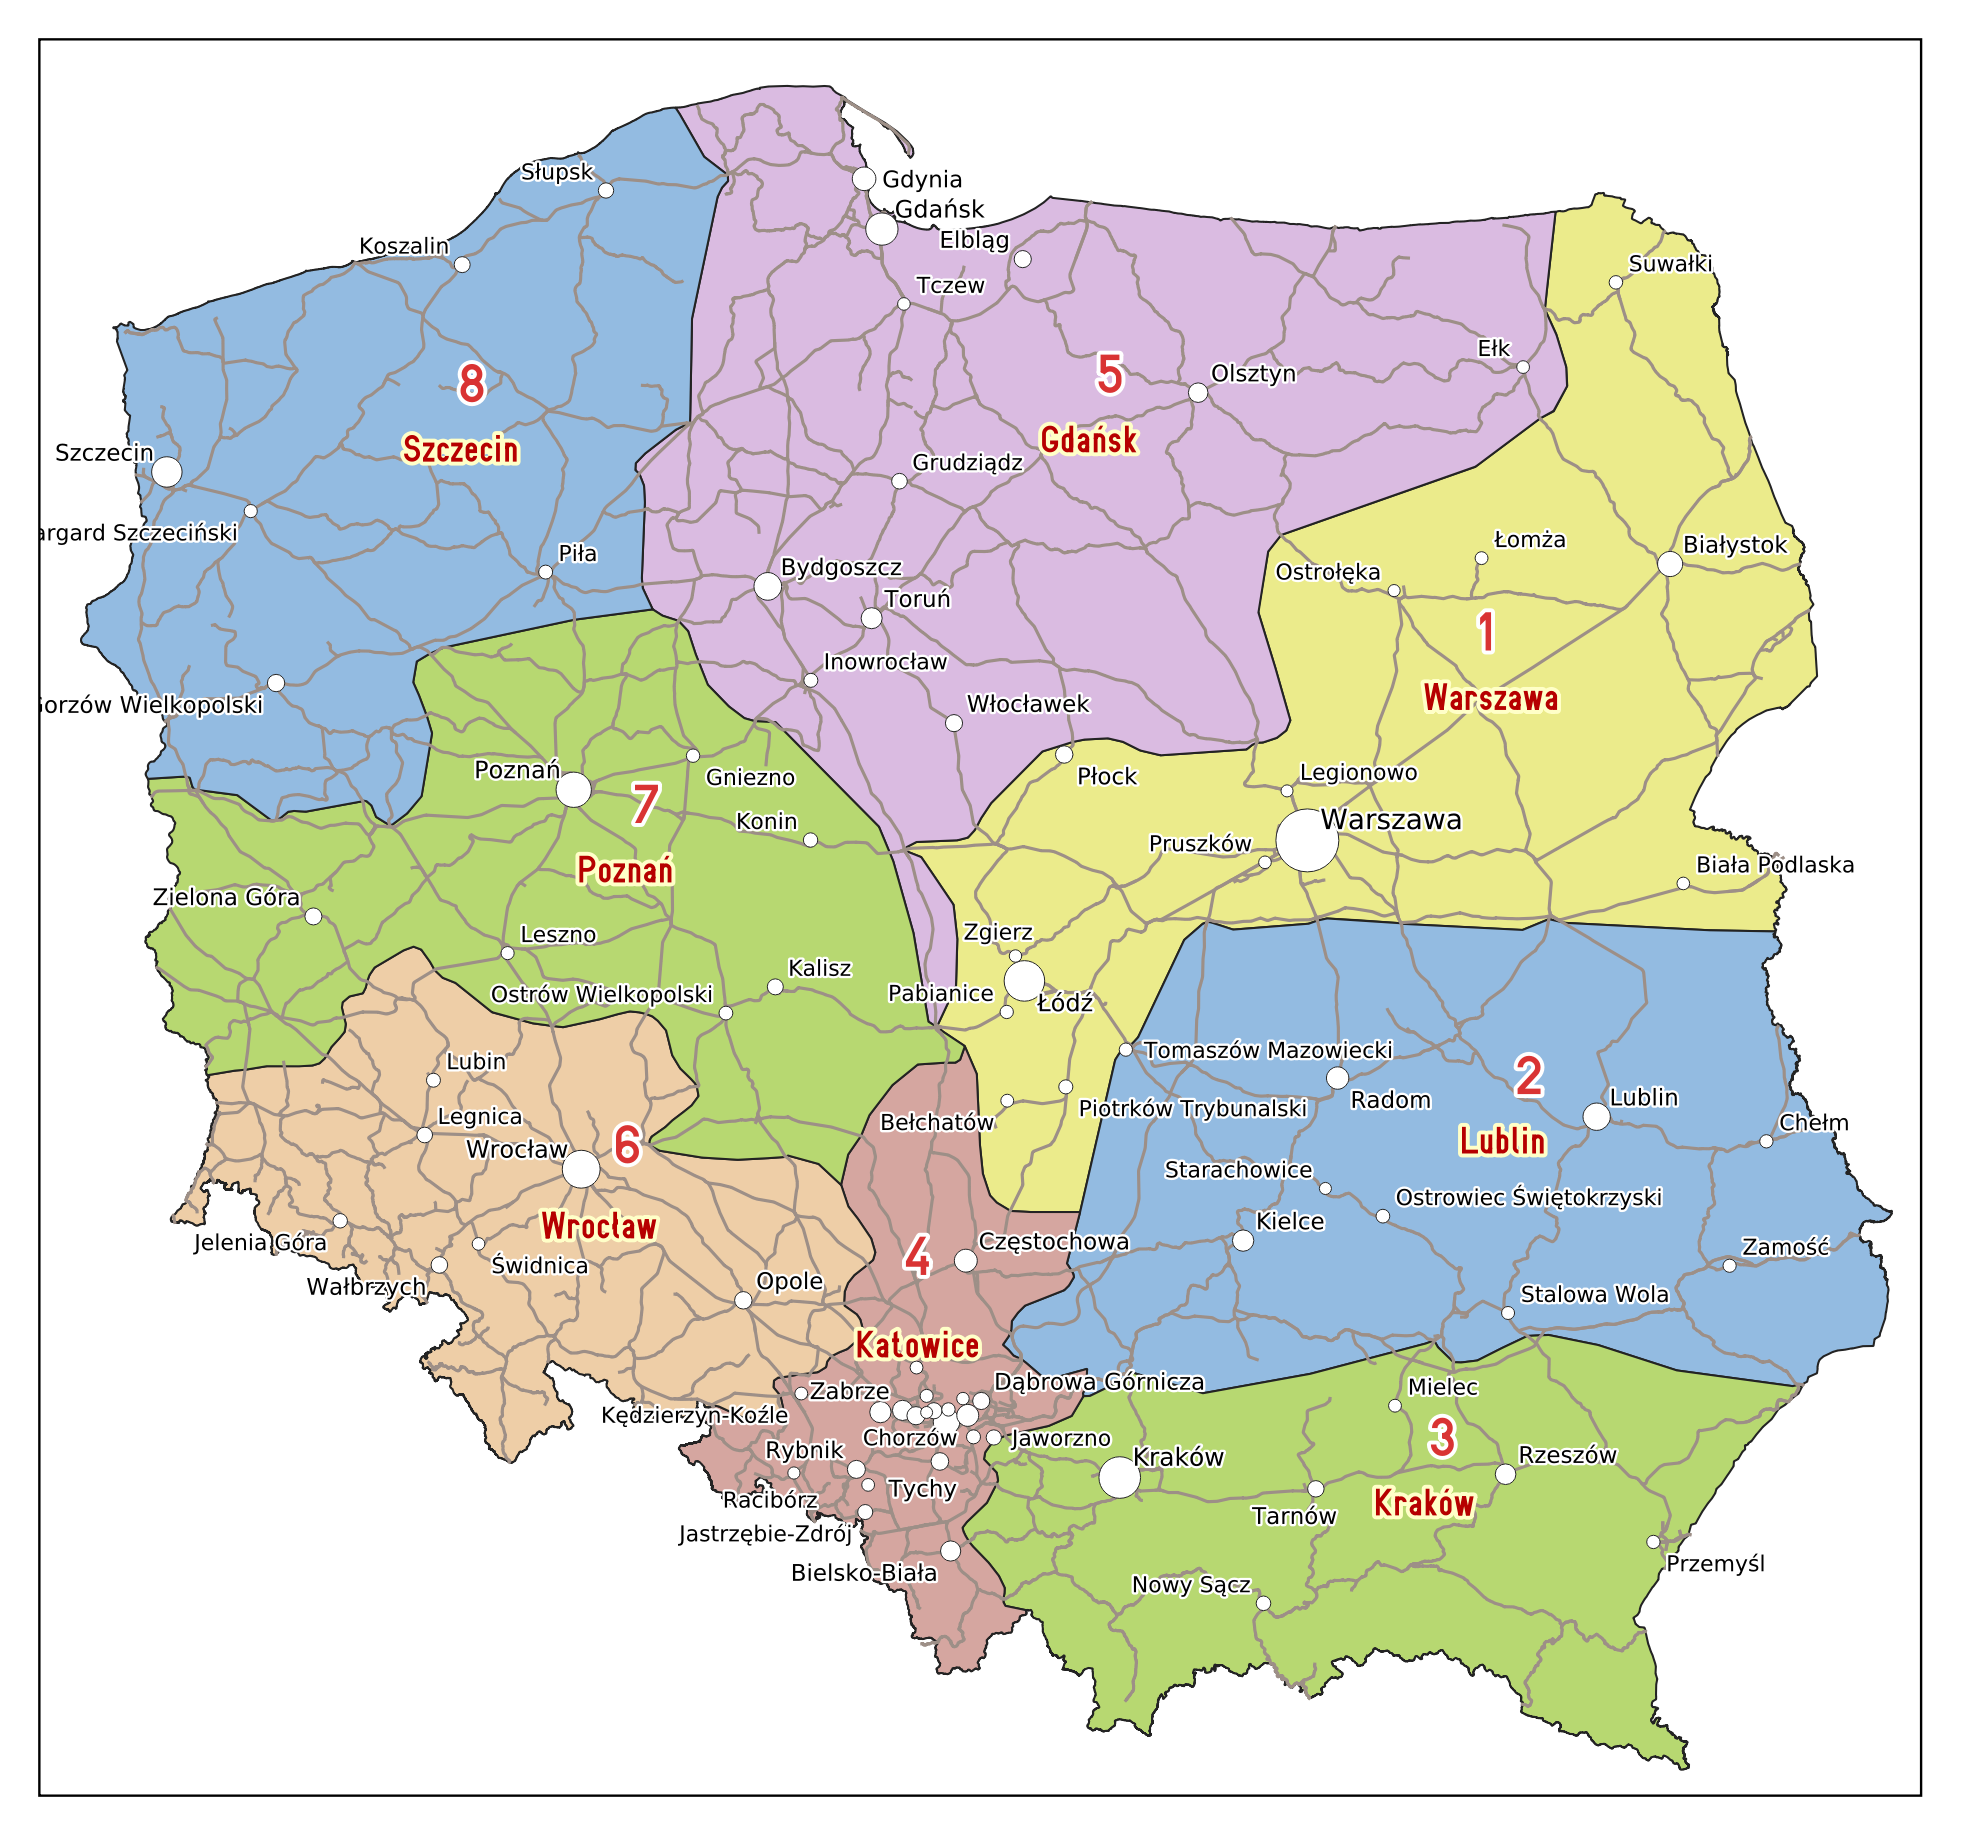
\includegraphics[width=12.5cm]{skryptkierownik-img/obszary-konstrukcyjne.png}	
	\caption{Obszary konstrukcyjne rozkładu jazdy}
\end{figure}

\chapter{Nadzór nad prowadzeniem i regulowaniem ruchu pociągów w sytuacjach nadzwyczajnych}

Rozkłady jazdy ustalane są tak, by zachowana została kolejność pierwszeństwa przejazdu według rodzaju i kategorii pociągów. 
Naczelną zasadą jest, że pierwszeństwo mają pociągi pasażerskie nad towarowymi. Rozpatrując pociągi pasażerskie to kryterium pierwszeństwa jest prędkość jazdy w związku z czym wyodrębnia się w kolejności od najwyższego stopnia pierwszeństwa pociągi: 
\begin{enumerate}
	\item nadzwyczajne specjalnego znaczenia, 
	\item kwalifikowane (EC, IC, Ex),
	\item pociągi pośpieszne,
	\item pociągi osobowe i aglomeracyjne dowożące ludzi do pracy, 
	\item pociągi osobowe i dalekobieżne i pozostałe miejscowe itd. 
\end{enumerate}
W sytuacjach nadzwyczajnych pierwszeństwo ponad wszystkimi z tych pociągów mają pociągi ratunkowe. Drezyny na blokadzie samoczynnej zawsze jako telefoniczne zapowiadanie pociągów. 

\chapter{Organizacja akcji ratunkowej w razie zdarzeń kolejowych i klęsk żywiołowych}

\section{Podstawowe pojęcia}

\textbf{Wydarzenie kolejowe} – każda niepożądana sytuacja zaistniała w systemie transportu kolejowego lub w jego otoczeniu zakłócająca realizację procesu przewozowego, w szczególności powodująca zagrożenie dla bezpieczeństwa ruchu kolejowego, opóźnienie pociągu lub zakłócenie prac manewrowych.
\\
\textbf{Wypadek} – niezamierzone nagłe zdarzenie lub ciąg takich zdarzeń z udziałem pojazdu kolejowego, powodujące negatywne konsekwencje dla zdrowia ludzkiego, mienia lub środowiska; 
do wypadków zalicza się w szczególności:
\begin{enumerate}
	\item kolizje;
	\item wykolejenia;
	\item zdarzenia na przejazdach;
	\item zdarzenia z udziałem osób spowodowane przez pojazd kolejowy będący w ruchu;
	\item pożar pojazdu kolejowego.
\end{enumerate}
\textbf{Poważny wypadek} – każdy wypadek spowodowany kolizją, wykolejeniem lub innym
zdarzeniem mającym oczywisty wpływ na regulacje bezpieczeństwa kolei lub na
zarządzanie bezpieczeństwem:
\begin{itemize}
	\item z przynajmniej \textbf{jedną} ofiarą \textbf{śmiertelną} lub przynajmniej \textbf{pięcioma ciężko rannymi};
	lub
	\item powodujący znaczne \textbf{zniszczenie pojazdu} kolejowego, infrastruktury kolejowej lub środowiska, które mogą zostać \textbf{natychmiast oszacowane} przez komisję badającą wypadek na co najmniej \textbf{2 miliony euro}.
\end{itemize}
\textbf{Znaczący wypadek} – wypadek z udziałem co najmniej jednego pojazdu kolejowego
będącego w ruchu:
\begin{itemize}
\item \textbf{z przynamniej jedną} ofiarą śmiertelną lub ciężko ranną;
lub
\item powodujący \textbf{znaczne szkody} w taborze, torach kolejowych, instalacjach lub
środowisku, tj. szkodę o wartości \textbf{co najmniej 150 tysięcy euro};
lub
\item powodujący znaczne zakłócenie ruchu, tj. wstrzymanie ruchu kolejowego na głównej linii kolejowej przez co najmniej 6 godzin.
\end{itemize}

\textbf{Incydent} – każde zdarzenie inne niż wypadek lub poważny wypadek, związane z ruchem kolejowym i mające wpływ na jego bezpieczeństwo.

\textbf{Sytuacja potencjalnie niebezpieczna} – sytuacja eksploatacyjna lub wydarzenie kolejowe niebędące poważnym wypadkiem, wypadkiem ani incydentem, powodujące nieznaczny wzrost ryzyka – do kontrolowanego poziomu nieprzekraczającego poziomu ryzyka akceptowalnego.

\section{Postępowanie przy zdarzeniu}
Postępowanie przy organizacji i prowadzeniu akcji ratunkowej określają instrukcje PKP PLK (Ir-8),instrukcje wewnętrzne KŚ (K-6, K-9), oraz procedura SMS P-16.
\\Pracownik kolejowy, który zauważył, że może dojść do zdarzenia, powinien użyć wszelkich możliwych środków, aby mu zapobiec, a gdy to jest niemożliwe, dążyć do ograniczenia jego skutków. 
W przypadku zabicia lub zranienia człowieka przez pojazd kolejowy, pojazd ten należy zatrzymać, a kierownik pociągu lub maszynista (albo ewentualnie inny pracownik kolejowy) zgłasza zdarzenie dyżurnemu ruchu na najbliższym posterunku ruchu zarządcy infrastruktury.
\marginnote{Instrukcja Ir-8, Rozdział II, \S.5}
\\Do czasu przybycia na miejsce zdarzenia naczelnika sekcji eksploatacji lub wyznaczonego przez niego pracownika, pracownik kolejowy, który zauważył zdarzenie, a w szczególności \textbf{kierownik pociągu}, czy prowadzący pojazd kolejowy, powinien:
\begin{enumerate}
	\item sprawdzić, czy na sąsiednich torach może odbywać się ruch pociągów (manewry).
	Jeżeli ruch nie może się odbywać, należy, o ile to możliwe, zabezpieczyć miejsce zdarzenia, a do zbliżających się pociągów podawać sygnał „Alarm”;
	\item poinformować dyżurnego ruchu na najbliższym posterunku ruchu zarządcy infrastruktury o dostrzeżonych zagrożeniach dla dalszego prowadzenia ruchu kolejowego, spowodowanych zaistniałym zdarzeniem;
	\item udzielić pierwszej pomocy poszkodowanym;
	\item przeciwdziałać powstaniu i rozprzestrzenianiu się pożaru;
	\item zabezpieczyć ślady mogące mieć znaczenie dla ustalenia przyczyn zdarzenia i nie dopuścić do ich zatarcia;
	\item zabezpieczyć mienie kolejowe, ładunki i bagaże pasażerów;
	\item informować dyżurnego ruchu o fakcie i czasie przybycia na miejsce zdarzenia służb	ratowniczych oraz ich rodzaju (pogotowie ratunkowe, straż pożarna, policja, zespół kolejowego ratownictwa technicznego itp.).
\end{enumerate}

\section{Pożar}
\marginnote{Instrukcja K-9, Rozdział II, \S.4, ust 1-9}
W razie powstania pożaru w pociągu należy pociąg ten niezwłocznie zatrzymać, podawać sygnał „Pożar”, wezwać podróżnych do opuszczenia palącego się wagonu i starać się ugasić pożar za pomocą posiadanych środków, w razie potrzeby przy pomocy podróżnych. Jeżeli nie można ugasić pożaru w zarodku, należy wezwać straż pożarną. Obowiązkowo o pożarze powiadomić dyżurnego ruchu, a w razie potrzeby miejsce niebezpieczne osłonić sygnałami i zażądać pomocy.

\section{Wykolejenie}
Wykolejenie jest to  trwała utrata kontaktu powierzchni tocznej koła pojazdu kolejowego z powierzchnią toczną główki szyny.
W razie wykolejenia, kierownik pociągu \textbf{natychmiast zawiadamia} dyżurnego ruchu najbliższego posterunku ruchu.
Gdy zajdzie taka potrzeba żąda przybycia karetki pogotowia, a rannym podróżnym, z udziałem pozostałych członków drużyny konduktorskiej - udziela pierwszej pomocy. Kierownik pociągu za każdym razem określa, czy wykolejone wagony nie stanowią zagrożenia dla bezpieczeństwa ruchu prowadzonego po torach sąsiednich. W razie zdarzenia kolejowego z udziałem pociągu z materiałami niebezpiecznymi, materiałami szczególnie niebezpiecznymi i wybuchowymi, kierownik pociągu bezwzględnie zawiadamia dyżurnego ruchu najbliższego posterunku ruchu informując go o tym fakcie i żądając wstrzymania ruchu na szlaku na którym nastąpił wypadek.
\marginnote{Instrukcja Ir-1, Rozdział 10, \S.76, ust 2}

Wagony wykolejone, nawet nie uszkodzone, powinny być zbadane przez \textbf{rewidenta} taboru kolejowego przed dopuszczeniem ich do dalszej jazdy w pociągu. W razie niemożności dokładnego zbadania wagonów wykolejonych na szlaku, po wstawieniu ich na tor, należy dowieźć je do najbliższej stacji, dostosowując prędkość jazdy do wskazówek rewidenta taboru kolejowego, przy czym prędkość ta nie może być większa niż 30 km/h.

\begin{tcolorbox}
	\begin{enumerate}
		\item Poważny wypadek to:
		\begin{enumerate}
			\item Wypadek spowodowany kolizją, wykolejeniem pociągu lub innym podobnym zdarzeniem z przynajmniej jedną ofiarą śmiertelną lub pięcioma rannymi,
			\item Wypadek spowodowany kolizją , wykolejeniem manewrującego taboru lub innym podobnym zdarzeniem,
			\item Wypadek spowodowany kolizją, wykolejeniem staczanego z górki rozrządowej taboru lub podobnym zdarzeniem.
		\end{enumerate}
		\item Wagony wykolejone na szlaku, przed dopuszczeniem ich do dalszej jazdy w pociągu, powinny być zbadane przez:
		\begin{enumerate}
			\item Kierownika pociągu,
			\item Maszynistę,
			\item Rewidenta taboru
		\end{enumerate}
		\item Zgłaszając wypadek kolejowy należy podać:
		\begin{enumerate}
			\item Miejsce i czas,
			\item Miejsce i jego skutki,
			\item Miejsce, czas i jego skutki
		\end{enumerate}
		\item Pracownik kolejowy, który zauważył zdarzenie, a w szczególności kierownik pociągu powinien:
		\begin{enumerate}
			\item Udzielić pierwszej pomocy rannym i unieruchomionym w wagonach,
			\item Zadbać o własne bezpieczeństwo,
			\item Powiadomić o zdarzeniu i oczekiwać na pomoc.
		\end{enumerate}
		\item W przypadku wykolejenia pociągu należy:
		\begin{enumerate}
			\item Wykolejony tabor wkoleić, dokonać oględzin technicznych i kontynuować jazdę,
			\item Pozostawić na miejscu wypadku wykolejony tabor i przynajmniej po jednym niewykolejonym wagonie z każdej strony,
			\item Pozostawić na miejscu wypadku wykolejony tabor.
		\end{enumerate}
	\end{enumerate}
	
\end{tcolorbox}

\chapter{Obowiązki manewrowego oraz nadzorującego i kierującego manewrami}

Kierownikiem manewrów może być: \textbf{ustawiacz, kierownik pociągu, dyżurny ruchu, nastawniczy, zwrotniczy}. 

Zespół pracowników zlożony z kierownika manewrów i co najmniej jednego pracownika manewrowego,  nazywa się drużyną
manewrową. Prowadzący pojazd kolejowy oraz pracownik posterunku nastawczego powinni zostać powiadomieni kto jest
kierownikiem manewrów. Pracownicy biorący udział w manewrach powinni znać regulaminy techniczne oraz pracy obsługiwanej
bocznicy kolejowej, dla rejonu w którym wykonują manewry.

Do obowiązków kierownika manewrów należy:

\begin{itemize}
\item ustalenie pracy manewrowej, omówienie z drużyną trakcyjną oraz obsługą posterunków nastawczych
\item podział czynności między manewrowych
\item sprawdzenie stanu zajętości i zamknięcia torów
\item sprawdzenie zabezpieczenia pojazdów kolejowych przed zbiegnięciem
\item sprawdzenie stanu i liczby płozów hamulcowych, oświetlenia i łączności
\item kierowanie rozrządzaniem i zestawieniem pociągów
\item dawanie sygnałów manewrowych
\item sprzęganie i rozprzęganie pojazdów
\end{itemize}
\ \ Kierownik manewrów może jednoosobowo wykonywać następujące manewry:

\begin{enumerate}
\item z włączonym hamulcem zespolonym
\end{enumerate}
\begin{itemize}
\item \begin{itemize}
\item przestawiać próżne składy pasażerskiego
\item przestawiać próżne zespoły trakcyjne – maszynista powinien prowadzić pojazd z pierwszej kabiny patrząc w kierunku
jazdy
\item wyciągać bez zmiany kierunku jazdy składy towarowe z torów przyjazdowych na wyciągowe, z torów kierunkowych na
odjazdowe.
\item Przestawiać z toru na tor składy nie przekraczające 60 osi rzeczywistych, na sygnały manewrowe na sygnalizatorach,
gdy pojazd trakcyjny i pracownik manewrowy posiadają sprawny radiotelefon, bez ograniczeń długości.
\end{itemize}
\end{itemize}
\begin{enumerate}
\item bez hamulca zespolonego przestawiać grupy wagonów do 8 osi rzeczywistych (ładowne), 28  osi rzeczywistych (próżne)
\item Nie wolno odrzucać pojazdów kolejowych w pojedyńczej obsadzie manewrowej
\end{enumerate}
\ \ Składy pociągów należy zostawić w stanie ściśniętych sprężyn zderzakowych, z zakręconym hamulcem ręcznym na
pierwszym i ostatnim wagonie.

\ \ Po zakończeniu manewrów, do obowiązków kierownika pociągu należy sprawdzenie czy pojazdy kolejowe znajdują się w
granicach ukresów oraz czy są należycie zabezpieczone przed zbiegnięciem.

\ \ Obowiązki manewrowego przed rozpoczęciem pracy:

\begin{itemize}
\item \begin{itemize}
\item \begin{itemize}
\item zgłoszenie się u kierownika manewtów, z przepisowym wyposażeniem (ochrona osobista i sygnałowe)
\item sprawdzenie stanu zapełnienia trów i które tory są wolne
\item czy pojazdy kolejowe są dopchnięte i połączone sprzęgami
\item czy pod kołami pojazdów nie ma płozów, lub innych przeszkód (np. wykolejnica)
\item czy na torach nie znajdują się pojazdy uszkodzone, wykolejone, z ładunkiem przesuniętym, uszkodzonym, lub pojazdy
wymagające zachownia szczególnej ostrożnością
\item sprawdzenie czy nie ma przeszkód na przejazdach kolejowo-drogowych (pojazdy, lód, piasek, zanieczyszczenia w
żłobkach)
\end{itemize}
\end{itemize}
\end{itemize}
\ \ W trakcie wykonywania manewrów obowiązki manewrowego to m.in.:

\begin{itemize}
\item \begin{itemize}
\item \begin{itemize}
\item rozprzęganie i sprzęganie pojazdów
\item przestawianie zwrotnic i wykolejnic przewidzianych do obsługi przez drużynę manewrową
\item dawanie sygnałów manewrowych
\item hamowanie manewrujących pojazdów
\item zabezpieczenie przed zbiegnięciem
\end{itemize}
\end{itemize}
\end{itemize}
\ \ Manewrowy może podawać sygnały przed dojechaniem do wagonów które ma połączyć, na polecenie kierownika manewrów,
albo celem wstrzymania manewrów w razie niebezpieczeństwa.

\ \ Po zakończeniu manewrów powinien sprawdzić czy nie pozostawiono pojazdów poza ukresem, zabezpieczyć pojazdy przed
zbiegnięciem, nieużyte płozy złożyć w wyznaczynm miejscu, pozawieszać sprzęgi hamulcowe na wsporniki.

\chapter{Sposoby wykonywania manewrów}

\textbf{\ \ Manewry} są to wszelkie zamierzone ruchy pojazdów kolejowych oraz związane z nimi czynności na torach, z wyjątkiem wjazdu, wyjazdu i przejazdu pociągów.
\marginnote{Instrukcja Ir-1, Rozdział II, par 11, pkt.1}

\ \ Manewry prowadzi się na trzy sposoby:

\begin{itemize}
\item \textbf{Odstawianie} polegające na przestawianiu pojazdów kolejowych na wyznaczony tor i odczepieniu po
zatrzymaniu, pojazdem trakcyjnym, podciągarką, przesuwnicą wagonową.
\item \textbf{Odrzucanie} polegające na tym że lokomotywa manewrowa pchając odprzęgnięte wagony, przy pewnej, określonej
prędkości zatrzymuje się, co powoduje że odprzęgnięte od niej wagony toczą się dalej samodzielnie na wyznaczony tor
\item \textbf{Grawitacyjny} polegający na staczaniu wagonów z gorki rozrządowej lub torów położonych na spadku
\end{itemize}

Wszelkie manewry należy wykonywać po uzgodnieniu z dyżurnym ruchu, oraz przerwać na każde jego żądanie. 

Bez drużyny manewrowej może odbywać się jazda manewrowa pojazdów pomocniczych, jazda manewrowa taboru specjalnego, jazda manewrowa pojazdów trakcyjnych bez doczepionego taboru, jazda manewrowa pojazdów trakcyjnych \textbf{ciągnących} nie więcej niż cztery wagony towarowe albo \textbf{dwa wagony} pasażerskie bez \textbf{podróżnych}, jazda manewrowa próżnych składów złożonych z zespołów trakcyjnych, przejazd ciągnionych składów pociągowych z torów przyjazdowych do innego rejonu stacji oraz z torów kierunkowych na tory odjazdowe, jazda manewrowa lokomotywy \textbf{pchającej} dwa wagony towarowe albo jeden \textbf{wagon pasażerski bez podróżnych}, gdy drużyna trakcyjna jest dwuosobowa, podstawienie pod perony \textbf{próżnych składów} pasażerskich prowadzonych z przedniej kabiny patrząc w kierunku jazdy.

Nie wolno odrzucać następujących wagonów:

\begin{itemize}
\item wagony z podróżnymi,
\item wagony salonowe, doświadczalne, laboratoryjne, pomiarowe, wagowe, podstacje elektryczne, inne służące różnym celom np.:
gospodarczym, socjalnym itp.
\item 
nieczynne pojazdy trakcyjne,
\item 
pojedyncze wagony ciężkie o masie brutto większej niż 120 ton,
\item wagony załadowane przesyłką przekraczającą skrajnię ładunkową lub przesyłką o masie ponad 60 ton w jednej sztuce oraz
wagony załadowane kontenerami wielkimi (o długości 6 m i większej),
\item wagony ogrzewcze, wagony z czynnym ogrzewaniem piecowym oraz wagony uszkodzone oznaczone nalepkami oznaczającymi
nieprzydatność wagonu do biegu na własnych kołach,
\item pojazdy specjalne np. żurawie kolejowe, maszyny do robót torowych, pługi odśnieżne itp.,
\item wagony bez ław pokrętnych z ładunkiem leżącym na dwu lub więcej wagonach (np.: długie szyny, pręty stalowe i inne długie
elastyczne przedmioty), 
\item wagony oznaczone nalepką ostrzegawczą nr 8 lub 15 według RID,
\begin{marginfigure}
	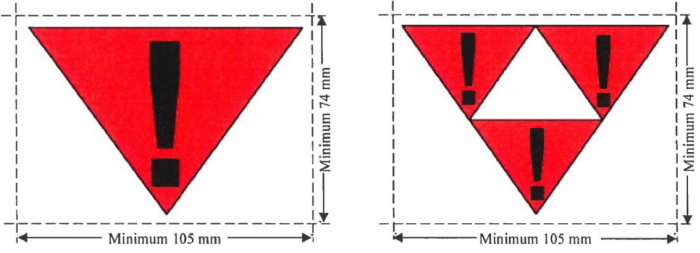
\includegraphics[width=5cm]{skryptkierownik-img/znaki-manewrowania.png}
	\caption{Nalepki ostrzegawcze nr 13 ostrożnie przetaczać oraz nr 15 zakaz odrzutu i staczania} 
	\end{marginfigure}
\item wagony cysterny oznaczone pasem koloru pomarańczowego, 
\item wagony do przewozu podróżnych, sypialne i restauracyjne oraz pocztowe i bagażowe.
\end{itemize}
Stałe oznaczenia i napisy ostrzegawcze na wagonach wymagających zachowania szczególnej ostrożności przy wykonywaniu nmanewrów

(kolor biały, umieszczone na ostojnicy z lewej strony):

\textbf{1. Znak ostrzegawczy}- zabroniony przejazd przez górkę rozrządową;
\begin{marginfigure}
	
\includegraphics[width=5cm]{skryptkierownik-img/skryptkierownik-img024.jpg}
	\caption{Znak ostrzegawczy - zakaz przejazdu przez górkę rozrządową}
\end{marginfigure}
{\color{black}
\textbf{2. Znak ostrzegawczy} - zabroniony przejazd przez górkę rozrządową o promieniu krzywizny (w płaszczyźnie pionowej) mniejszym, niż podany pod znakiem;}
\begin{marginfigure}
	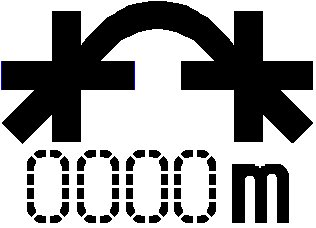
\includegraphics[width=4.5cm]{skryptkierownik-img/skryptkierownik-img025.jpg}
	\caption{Znak ostrzegawczy - zabroniony przejazd przez górkę o promieniu krzywizny}
\end{marginfigure}
\textbf{3. Znak ostrzegawczy}- dopuszcza się przetaczanie przez górkę rozrządową tylko przy zachowaniu szczególnych środków ostrożności:
\begin{marginfigure}
	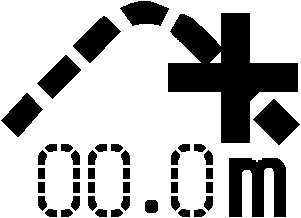
\includegraphics[width=4.5cm]{skryptkierownik-img/skryptkierownik-img026.jpg}
	\caption{Znak ostrzegawczy - zachowanie ostrożności}
\end{marginfigure}

Na tor \textbf{prawy} - zasadniczy szlaku dwutorowego przy ruchu dwutorowym jednokierunkowym zezwolenie \textbf{ustne} wykonania manewrów może udzielić dyżurny ruchu. Na tor \textbf{przeciwny} do zasadniczego zezwolenie wykonania manewrów musi być udzielone na podstawie \textbf{rozkazu pisemnego ''S''}. Zezwolenie takie może być wydane na wielokrotne jazdy w ściśle określonym obrębie czasu. Każdorazowo poza zezwoleniem musi być podany sygnał manewrowy podawany na sygnalizatorze lub sygnał ręczny "Do mnie".

\chapter{Sygnały podawane przy manewrach}

\section{Tarcze manewrowe świetlne i kształtowe}
Podstawowe sygnały manewrowe Ms1 i Ms2 podawane są przy pomocy tarcz manewrowych świetlnych. Na niektórych posterunkach mogą istnieć również tarcze manewrowe kształtowe lub nieruchome. Jeśli występuje tarcza manewrowa nieruchoma, podająca sygnał ''M1 Jazda manewrowa zabroniona'', należy pojazd kolejowy zatrzymać przed tarczą, a dalszą jazdę manewrową można kontynuować na polecenie ustne dyżurnego ruchu i sygnał Rm1 ''Do mnie''.
\begin{marginfigure}
	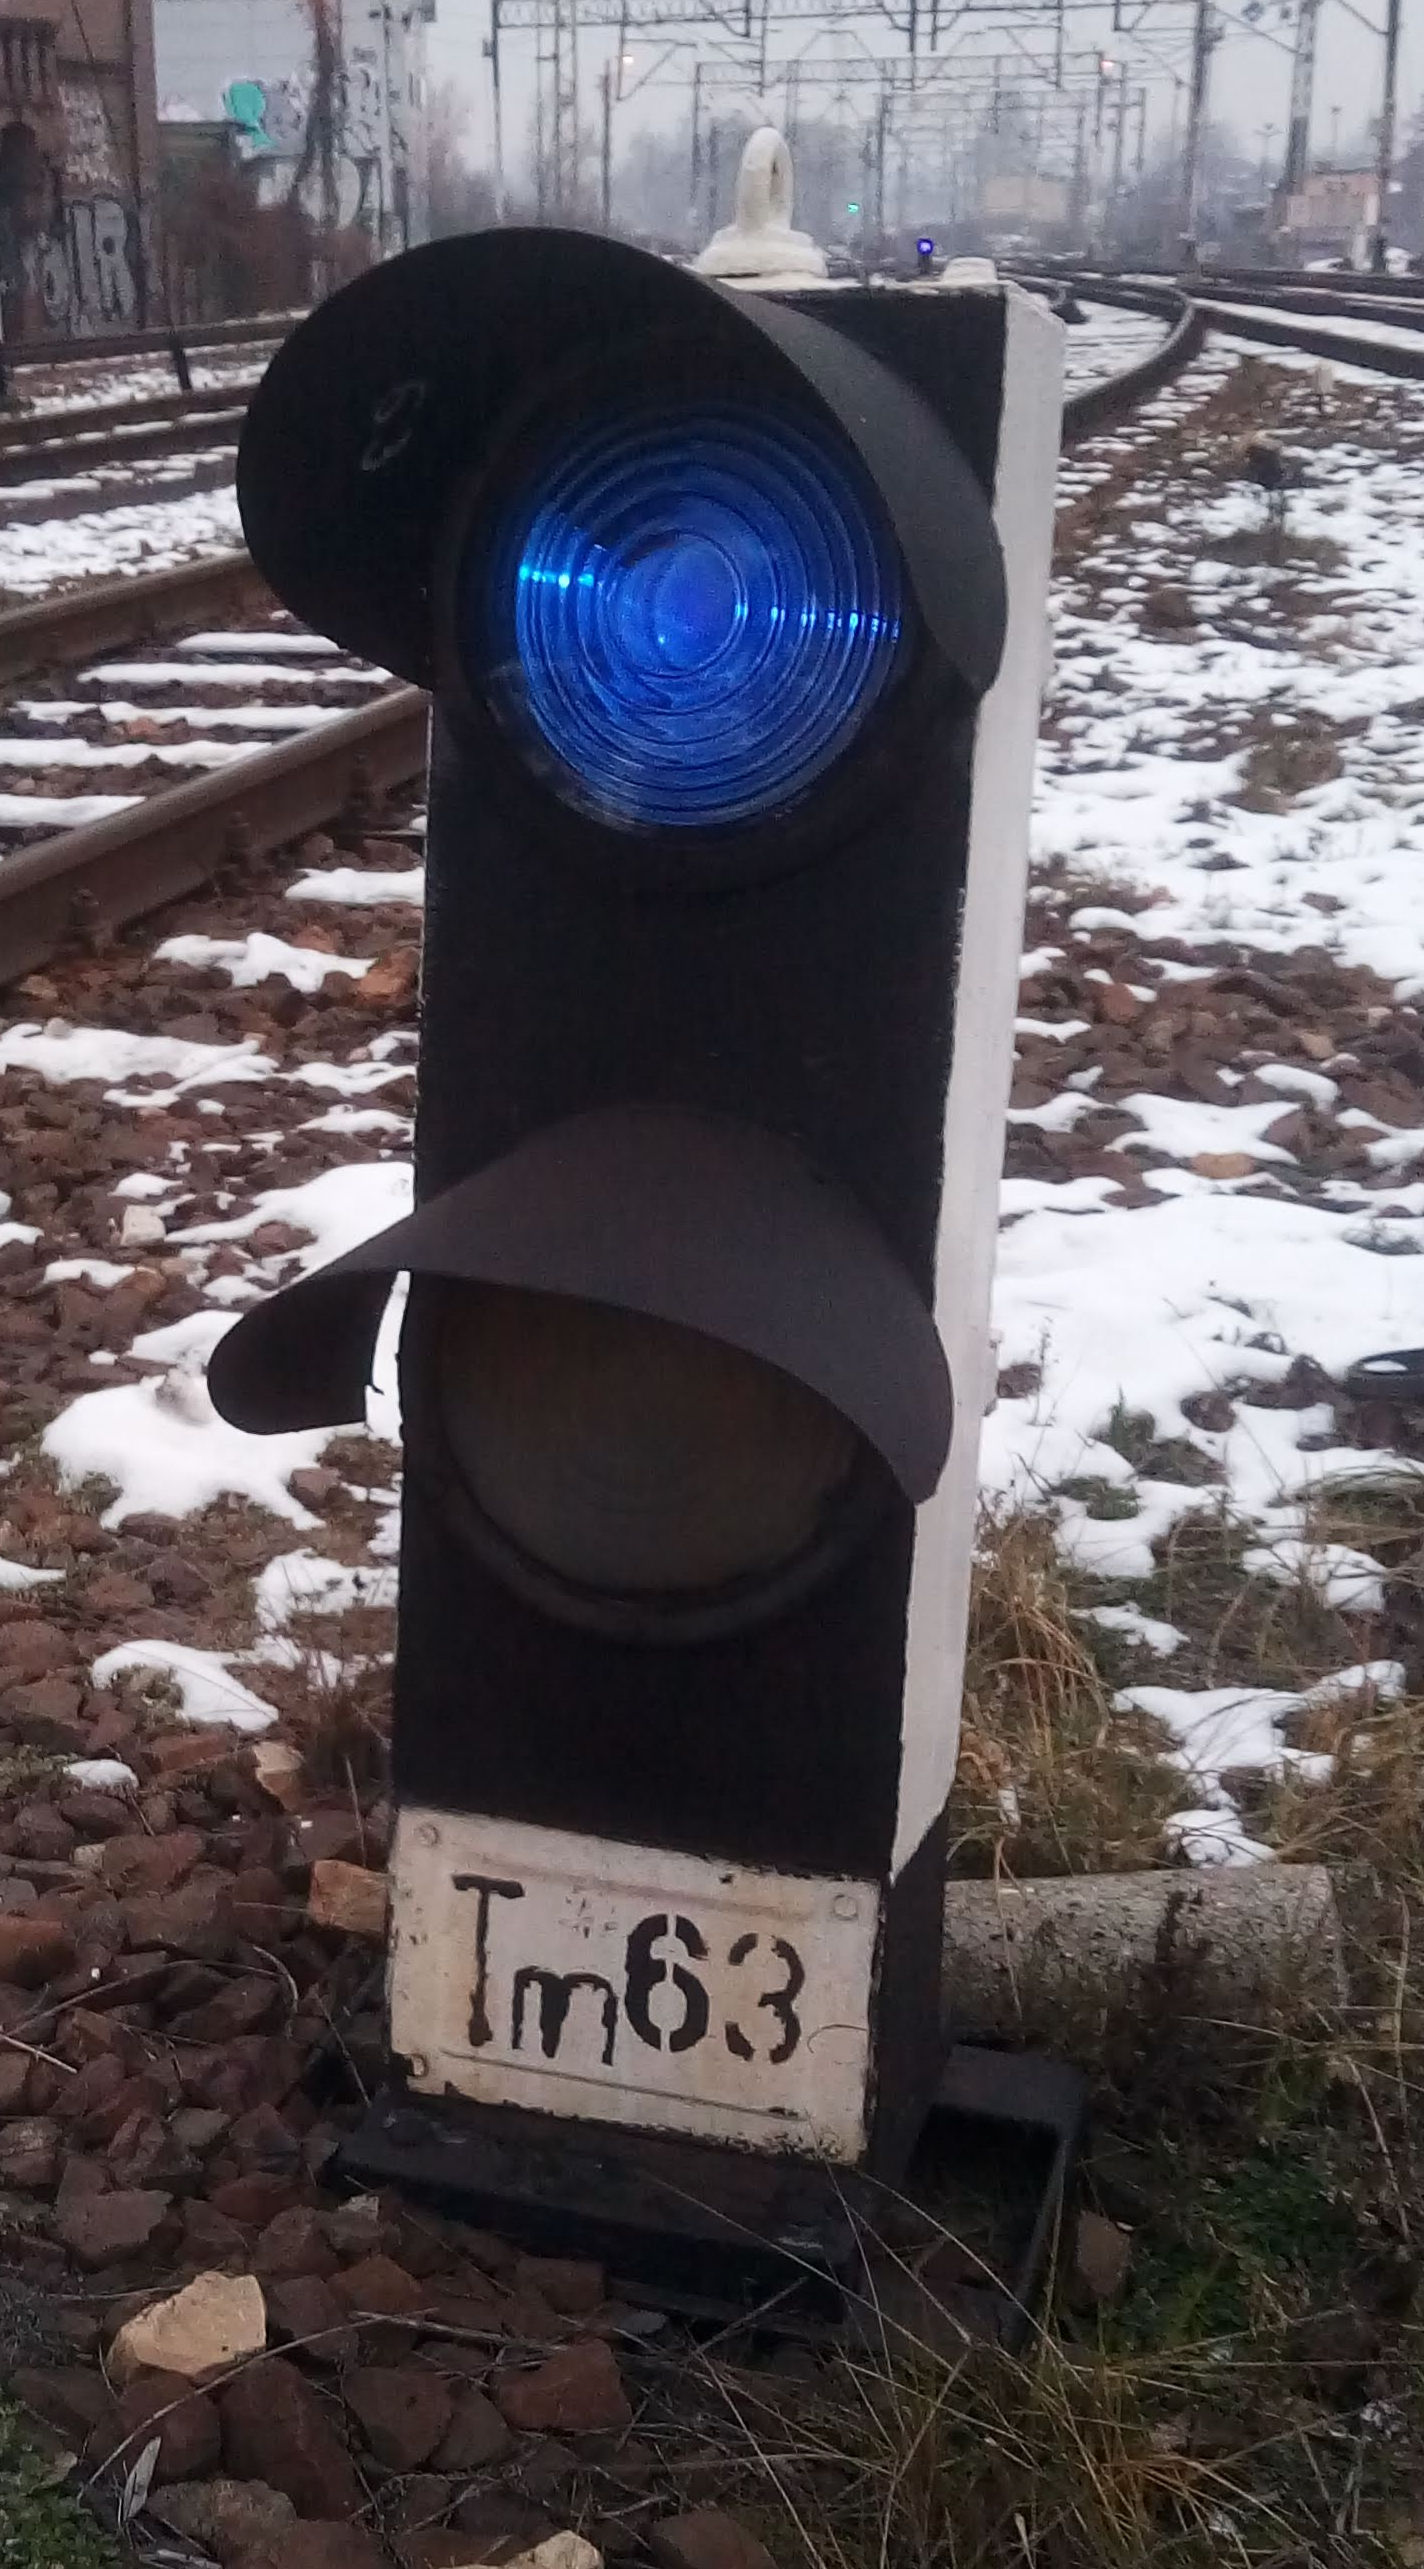
\includegraphics[width=4.5cm]{skryptkierownik-img/tarcza-manewrowa-ms1.jpg}
	\caption{Tarcza manewrowa karzełkowa wskazująca sygnał Ms1}
\end{marginfigure}
 W przypadku tarcz kształtowych ruchomych, oraz sygnalizatorów świetlnych, zezwoleniem na wykonywanie manewrów taboru jest sygnał ''Ms2 Jazda manewrowa dozwolona'' (jedno matowobiałe światło na tarczy/semaforze). Jeśli nie można na sygnalizatorze nastawić sygnału M2 lub Ms2, manewrujący może przejechać poza sygnalizator zabraniający dalszej jazdy, gdy upoważniony pracownik da zezwolenie na jazdę (ustnie, radiotelefonicznie) oraz sygnał odpowiednio Rm1 ''Do mnie'' lub Rm2 ''Ode mnie''.

\section{Semafory półsamoczynne lub tarcze zaporowe}
Na semaforach półsamoczynnych przystosowanych do podawania sygnałów manewrowych (oznaczonych literą m na tabliczce z nazwą semafora) istnieje możliwość podania sygnału Ms2. Sygnału Ms1 nie wyświetla się na takim semaforze, w jego miejsce podawany jest sygnał S1 ''Stój''

\section{Sygnały ręczne i dźwiękowe}
\subsection{Rm1 Do mnie}
Sygnał ''Do mnie'' podaje się chorągiewką sygnałową koloru żółtego lub ręką poruszaną poziomo, oraz przy pomocy gwizdawki - dwa długie tony.

\subsection{Rm2 Odemnie}
Sygnał ''Ode mnie'' podaje się chorągiewką sygnałową koloru żółtego lub ręką poruszaną pionowo, oraz przy pomocy gwizdawki - jeden długi ton.
\subsection{Rm3 Zwolnić}
Sygnał ''Zwolnij'' podaje się chorągiewką sygnałową koloru żółtego lub ręką poruszaną po łuku do góry i na dół, oraz przy pomocy gwizdawki - kilka przeciągłych tonów.
\subsection{Rm6 Docisnąć}
Sygnał ''Docisnąć'' podaje się poprzez kilkukrotne zbliżenie do siebie wyciągniętych poziomo przed siebie rąk, oraz przy pomocy gwizdawki - dwa krótkie tony.
\subsection{Rm4 Stój}
Sygnał ''Stój'' podajemy wykonując okrężny ruch wyprostowaną reką, chorągiewką sygnałową, lub w nocy latarką, oraz przy pomocy gwizdawki podając wielokrotnie trzy krótkie dźwięki. Sygnał ''Stój'' podaje się aż do całkowitego zatrzymania pojazdu.

\chapter{Prędkości jazd manewrowych i pociągowych}

\begin{table}
\begin{tabular}{|m{10cm}|m{5cm}|}
\hline
Opis &
Prędkość dopuszczalna\\\hline
Zasadnicza prędkość~manewrowa &
25 km/h\\\hline
Jazda manewrowa po torze wolnym (bez rozjazdów), po omówieniu pracy manewrowej &
40 km/h\\\hline
Wyjazd na sygnał zastępczy na szlak z półsamoczynną blokadą liniową (do granicy posterunku) &
40 km/h\\\hline
Cofanie pociągu ze szlaku po uzgodnieniu z dyżurnym ruchu &
30 km/h\\\hline
Jazda pociągu na tor zamknięty - bez przeszkody, po otrzymaniu tej informacji na rozkazie pisemnym S &
z prędkością rozkładową\\\hline
Jazda pociągu na tor zamknięty - zajęty (z przeszkodą) &
30 km/h\\\hline
Przez niezabezpieczone przejazdy i przejścia &
20 km/h\\\hline
Na torze zamkniętym, na 500m przed przeszkodą &
20 km/h\\\hline
Wyjazd na sygnał zastępczy na szlak z samoczynną blokadą liniową (do następnego semafora) &
20 km/h\\\hline
Wjazd do stacji na tor zakończony kozłem oporowym, lub niedostępny w części &
20 km/h\\\hline
Manewry na tor częściowo zajęty &
20 km/h\\\hline
Jazdy składu manewrowego pojazdami kolejowymi naprzód po torze głównym o spadku ponad 2,5\textperthousand, a pojazd trakcyjny nie mógł być umieszczony od strony spadku &
15 km/h\\\hline
Z podróżnymi, z towarami niebezpiecznymi, z przesyłką nadzwyczajną &
10 km/h\\\hline
Dojeżdżanie odsprzęgów staczanych z górki do stojącego taboru &
5,4 km/h\\\hline
Nieuzgodnione cofanie pociągu ze szlaku poprzedzone w drodze hamowania przez pracownika drużyny &
5 km/h\\\hline
Na sygnał „ pchać z umiarkowaną szybkością”, przy rozprzęganiu drążkiem, przy przetaczaniu wagonów oznaczonych nalepką ostrzegawczą 8 lub 15 wg RID oraz cystern z pasem koloru pomarańczowego, jeśli pracownik manewrowy porusza się przedskładem &
5 km/h\\\hline
Na sygnał „pchać powoli”, przy dojeżdżaniu lokomotywy do stojącego taboru, przy przetaczaniu za pomocą urządzeń
mechanicznych &
3 km/h\\\hline
Przy dojeżdżaniu do stojących pojazdów kolejowych &
3 km/h\\\hline
\end{tabular}
\end{table}
\chapter{Manewry po torach głównych oraz przez przejazdy i przejścia}

Manewry po torach głównych można wykonywać wyłącznie za zgodą dyżurnego ruchu nastawni dysponującej. Wyjazd manewrującego taboru na szlak (w kierunku szlaku) poza
wskaźnik oznaczający granicę przetaczania, a gdzie wskaźnika takiego nie ma – poza ostatni rozjazd (skrzyżowanie torów),dozwolony jest tylko za zezwoleniem dyżurnego ruchu.

W przypadku wyjazdu na tor (w kierunku toru):

– szlaku jednotorowego,

– lewy szlaku dwutorowego (w kierunku przeciwnym do zasadniczego),

– prawy szlaku dwutorowego (w kierunku zasadniczym), po którym prowadzony jest ruch dwukierunkowy,

– w kierunku przeciwnym do zasadniczego szlaku wielotorowego,

– w kierunku zasadniczym, po którym prowadzony jest ruch dwukierunkowy szlaku wielotorowego, zezwolenie to musi być przekazane rozkazem pisemnym „S”

\ \ Na tor prawy (\textbf{zasadniczy}) szlaku \textbf{dwutorowego}, gdy prowadzony jest po nim ruch \textbf{jednokierunkowy} jazda za wskaźnik granicy przetaczania możliwa jest na ustne zezwolenie dyżurnego ruchu.

Manewry przez przejazdy i przejścia kolejowo-drogowe należy prowadzić przy zamkniętych rogatkach. Jeśli przejazd/przejście nie jest chronione, prędkość manewrowania nie powinna przekraczać 20km/h, przy zbliżaniu się do przejazdu należy podawać sygnał Baczność, a w przypadku pchania pojazdów kolejowych, manewrowy powinien znajdować się na pierwszym pojeździe lub poprzedzać go oraz podawać odpowiednie sygnały.



	
	\part{Tabor}
	\part{Tabor}

\chapter{Ogólne zasady przewozu przesyłek nadzwyczajnych}
Zasady przewozu przesyłek nadzwyczajnych na sieci PKP PLK określa instrukcja Ir-10

\textbf{Skrajnia budowli} - zarys figury płaskiej stanowiący podstawę do określenia wolnej przestrzeni dla ruchu pojazdów szynowych, na zewnątrz którego powinny znajdować się wszelkie budowle, urządzenia i przedmioty położone przy torze, z wyjątkiem urządzeń przeznaczonych do bezpośredniego współdziałania z torem, jak np. hamulce torowe w stanie roboczym i przewody jezdne.

\begin{marginfigure}
	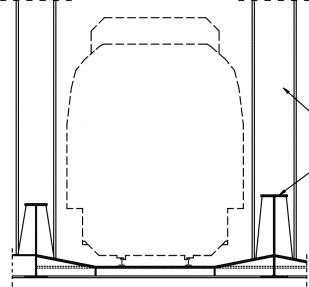
\includegraphics[width=5cm]{skryptkierownik-img/skrajnia.jpg}
	\caption{Przykładowa skrajnia taboru}
\end{marginfigure}
\textbf{Skrajnia taboru} - zarys figury płaskiej, stanowiący podstawę do określania największych dopuszczalnych wymiarów taboru w przekroju poprzecznym.

\textbf{Skrajnia ładunkowa} - zarys figury płaskiej, stanowiący podstawę do określania największych dopuszczalnych wymiarów ładunku spoczywającego na wagonie – pionowych licząc od górnej powierzchni główki szyny oraz poziomych licząc od osi toru.

Skrajnie dzieli się na krajową (ruchu wewnętrznego) i międzynarodową (wszystkie rodzaje pojazdów szynowych z wyjątkiem elektrycznych pojazdów trakcyjnych).

\textbf{Przesyłka nadzwyczajna} - to takie rzeczy lub pojazdy, których przewóz może powodować trudności w przewozie koleją i wymaga zachowania szczególnych warunków techniczno-ruchowych ze względu na: 

\begin{enumerate}
	\item kształt, rozmiary lub masę,
	\item sposób załadowania, rozmieszczenia i zabezpieczenia na wagonie,
	\item użyte środki przewozowe,
	\item drogę przewozu.
\end{enumerate}

Przesyłkę nadzwyczajną w komunikacji krajowej stanowią:

\begin{enumerate}
	\item rzeczy:
	\begin{enumerate}
		\item \textbf{przekraczające} określoną \textbf{skrajnię} ładunkową lub załadowane z przekroczeniem tej skrajni \textit{(szerokość lub wysokość ładunku po umieszczeniu na wagonie, jest większa niż wymiary skrajni ładunkowej)},
		\item wymagające specjalistycznego wagonu, urządzeń, zabezpieczenia bądź szczególnej organizacji przewozu ze względu na położenie środka ciężkości lub inne przyczyny związane z bezpieczeństwem przewozu,
		\item wymagające przewozu w wagonach z zagłębioną podłogą,
		\item o masie jednej sztuki \textbf{ponad 60 t},
		\item powodujące obciążenie na oś wagonu lub metr bieżący toru większe od dopuszczalnego choćby w części drogi przewozu,
		\item wymagające załadowania co najmniej na dwa wagony z ławami pokrętnymi, nie połączone ze sobą sprzęgami wagonowymi lub wagonem pośrednim,
		\item szyny, pręty stalowe do zbrojenia betonu oraz metale giętkie o długości \textbf{ponad 36 m}, ładowane na co najmniej dwa wagony bez ław pokrętnych,
	\end{enumerate}
	\item pojazd kolejowy toczący się na własnych kołach będący sam przedmiotem umowy przewozu lub załadowany przesyłkami:
	\begin{enumerate}
		\item \textbf{ bez znaków RIV, TEN lub RIC}
		\item bez znaków MC,
		\item \textbf{bez świadectwa dopuszczenia} do eksploatacji wydanego przez właściwy organ,
		\item specjalistyczne pojazdy kolejowe np. dźwigi, maszyny torowe i drogowe. Wyjątek stanowią pojazdy kolejowe do wykonywania przewozów technologicznych oraz wieloczynnościowe i ciężkie maszyny do robót budowlanych Zarządcy. Przewozy te realizowane są na podstawie oddzielnych regulaminów opracowanych przez właściwe jednostki Zarządcy, użytkujące te pojazdy,
		\item o średnicy kół \textbf{mniejszej niż 840 mm}, w tym również oznaczony znakami RIV, TEN, RIC lub MC
		\item o przekroczonej skrajni taboru
	\end{enumerate}
\end{enumerate}

Decyzję o zgodzie na przewóz przesyłki nadzwyczajnej podejmuje Zarządca infrastruktury na wniosek Przewoźnika.

\chapter{Ogólne zasady przewozu przesyłek niebezpiecznych}

Zasady przewozu towarów niebezpiecznych określa instrukcja Ir-16

\textbf{Numer UN}– międzynarodowy czterocyfrowy numer towaru niebezpiecznego.

\textbf{RID} – Regulamin międzynarodowego przewozu kolejami towarów niebezpiecznych.
\marginnote{Règlement concernant le transport international ferroviaire des marchandises dangereuses - załącznik do umowy o Międzynarodowej Kolejowej Komunikacji Towarowej (SMGS)}

\textbf{Towary niebezpieczne (TN)} – materiały i przedmioty, których przewóz transportem kolejowym jest zabroniony, albo
dopuszczony na ściśle określonych warunkach, zawartych w przepisach RID

Towary niebezpieczne stanowią materiały i przedmioty, które ze względu na właściwości fizyczne, chemiczne lub biologiczne, stwarzają potencjalne zagrożenie bezpieczeństwa w przypadku niewłaściwego obchodzenia się z nimi w czasie przewozu lub w przypadkach zaistnienia wydarzenia, mogące powodować śmierć, zagrożenie zdrowia, zniszczenie środowiska naturalnego lub dóbr materialnych.

\textbf{Towary niebezpieczne wysokiego ryzyka TWR} -  jest to grupa towarów wyodrębniona z towarów niebezpiecznych, które użyte niezgodnie ze swoim przeznaczeniem, tj. do celów terrorystycznych mogą spowodować poważne skutki, takie jak liczne ofiary, masowe zniszczenia lub szczególnie w przypadku klasy 7, masowe zakłócenia społeczno – gospodarcze.

Oznakowanie przesyłek niebezpiecznych:
\begin{marginfigure}
	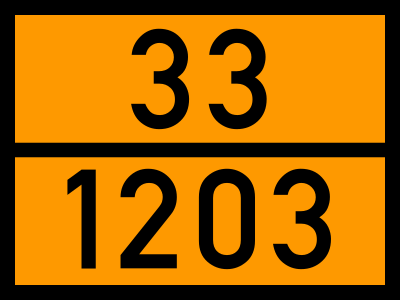
\includegraphics[width=5cm]{skryptkierownik-img/tablica-adr.png}
	\caption{Tablica z symbolami niebezpieczeństwa i substancji, źródło: Wikipedia}
	\label{fig:adr}
\end{marginfigure}	
Na każdej ścianie bocznej wagonu, cysterny, kontenera przewożącego towary niebezpieczne musi być umieszczona \textbf{tablica pomarańczowa}, o wymiarach 40x30 cm, z czarną obwódką. 

W górnej części tablicy znajduje się numer zagrożenia.

W dolnej części znajduje się numer UN.

Jeżeli zagrożenie stwarzane przez dany materiał może być wystarczająco określone jedną cyfrą, wówczas po tej cyfrze stawia się zero.

Podwojenie pewnej cyfry wskazuje na nasilenie odpowiedniego zagrożenia.

Jeżeli numer zagrożenia jest poprzedzony literą „X” oznacza to, że materiał niebezpiecznie reaguje z wodą

Obowiązek umieszczenia tablicy pomarańczowej dotyczy również przewozu próżnych nieoczyszczonych, nieodkażonych oraz nieodgazowanych jednostek transportowych po materiałach niebezpiecznych.
\begin{marginfigure}
	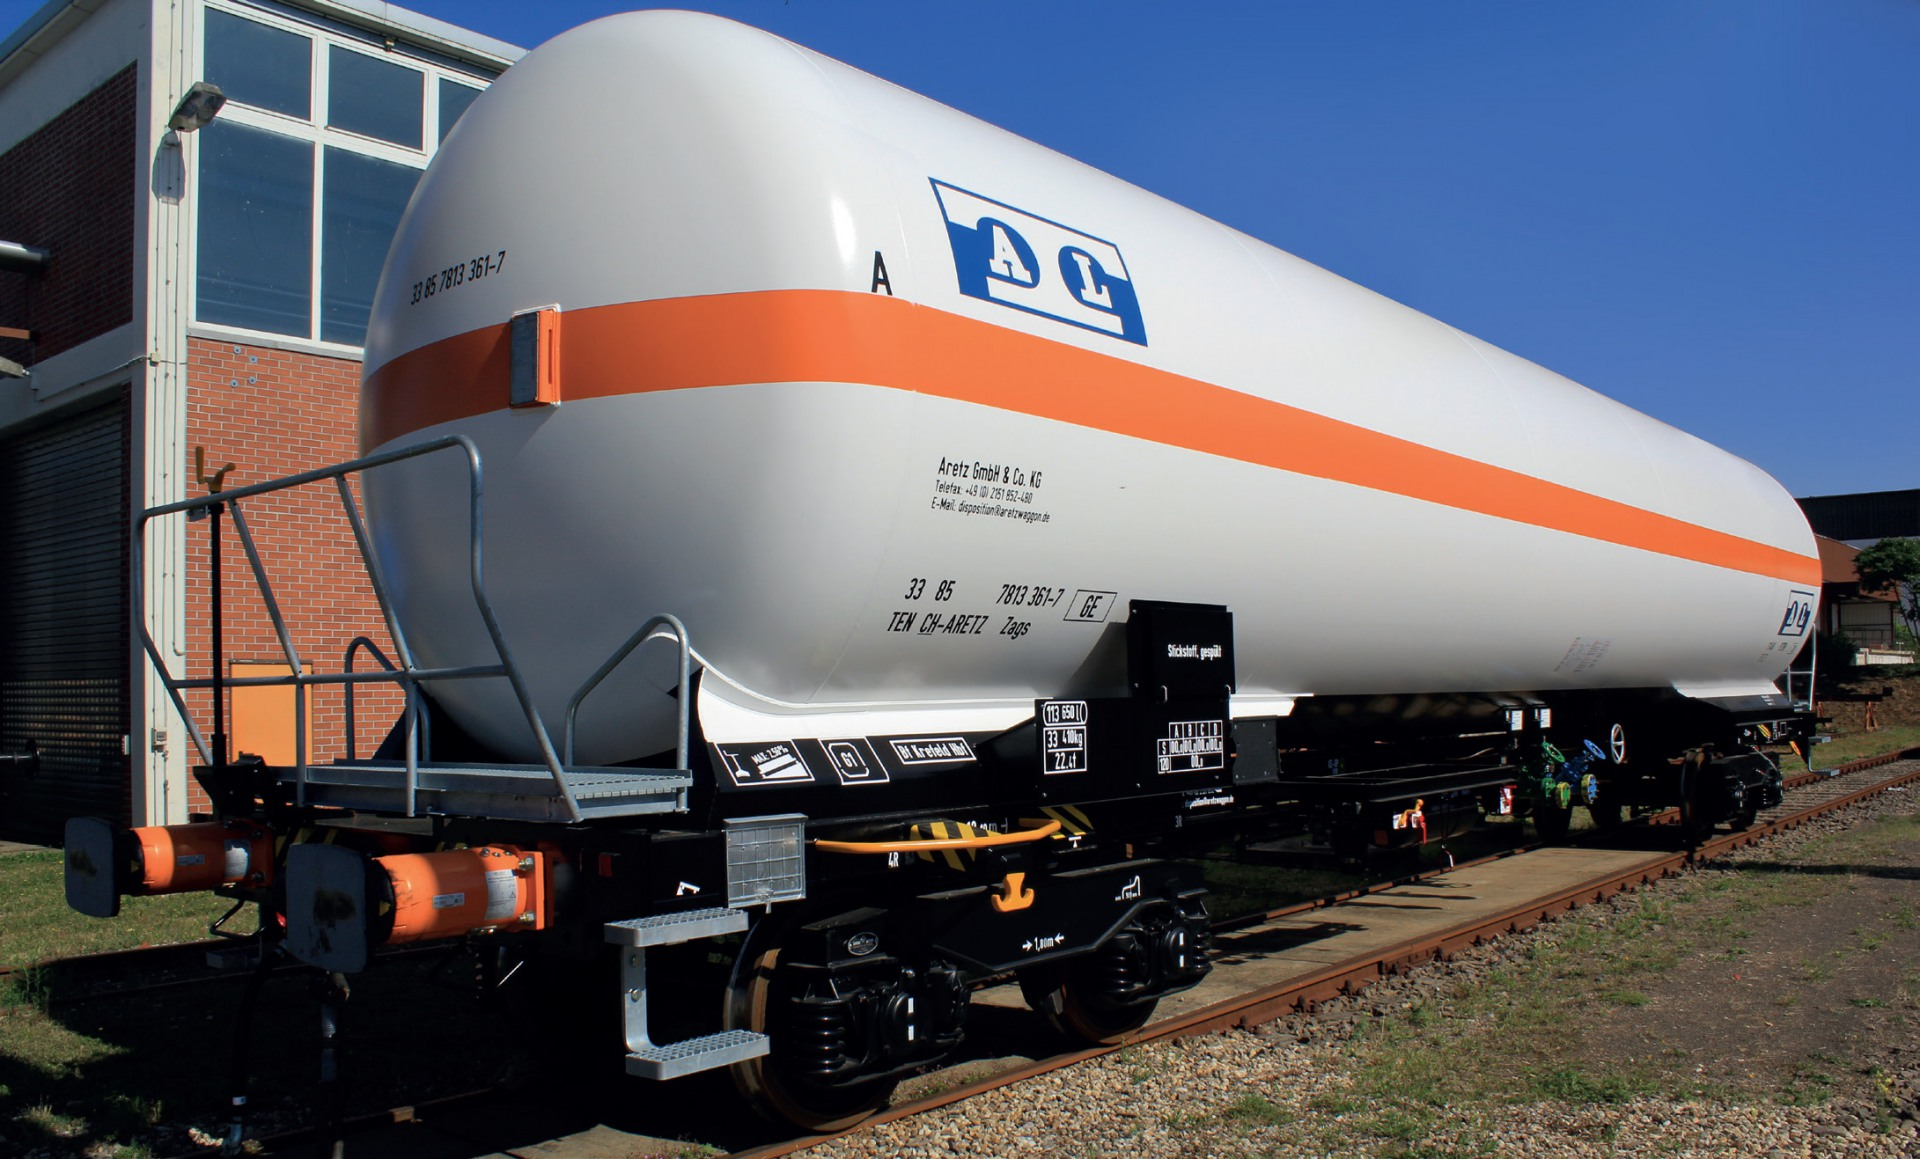
\includegraphics[width=5cm]{skryptkierownik-img/cysterna-rid.jpg}
	\caption{Cysterna do przewozu gazów, za: http://chemet.com.pl}
	\label{fig:cysterna}
\end{marginfigure}
\textbf{Pas} o szerokości ok. 30 cm\textbf{ koloru pomarańczowego} nieodblaskowego na cysternach przeznaczonych do przewozu gazów skroplonych, skroplonych schłodzonych lub rozpuszczonych. Wagony “szerokotorowe” mogą mieć pasy innego koloru dla przewozu specyficznych substancji.

\textbf{Nalepki ostrzegawcze}, umieszczane na opakowaniach, pojemnikach, kontenerach, wagonach, cysternach. Nalepka musi mieć kształ rombu, o wymiarach conajmniej 100 mm dla opakowań i conajmniej 250 mm dla wagonów. Wzory i kolory nalepek
związane są z klasą niebezpieczeństwa, opisane są w części 5 RID.


\chapter{Budowa taboru pasażerskiego}
	\section{Wózek}

Wózki służą do przeniesienia ruchu obrotowego kół na pudło, oraz ustabilizowanie tego ruchu. Pierwsze konstrukcje pojazdów kolejowych posiadały wagony dwuosiowe, bez wózków, z mocowaniem maźnicy zestawu kołowego bezpośrednio do ostoji wagonu. Obecnie większość wagonów wyposażona jest w dwuosiowe wózki które lepiej wpisują się łuki toru. Niektóre lokomotywy, oraz tabor specjalistyczny wyposażone są w wózki trzy- lub wielo-osiowe. Najbardziej rozpowszechnionym typem konstrukcji jest rama skrzynkowa do której montowane są pozostałe elementy wózka.

Wyróżnia się wózki toczne (nie posiadające napędu – wagonowe) i napędowe. Wózki napędowe w lokomotywach elektrycznych i spalinowych z przekładnią elektryczną mają zabudowane silniki(zwykle – 1 silnik na 1 oś). Istnieją (rzadkie) przykłady wózków napędowych bez silników, w których następuje jedynie zamiana ruchu obrotowego wału dostarczającego moc z silnika umieszczonego w pudle lokomotywy na ruch obrotowy kół za pomocą przekładni (rozwiązanie stosowane w spalinowozach z przekładnią mechaniczną). Istnieją też wózki, w których niektóre osie są napędowe, a niektóre toczne (np. lokomotywy spalinowe).

W wózku zabudowane są elementy zapewniające usprężynowanie pojazdu szynowego. Pojazdy służące do przewozu podróżnych cechują się wyposażeniem w dwa stopnie usprężynowania. Dawniej najczęściej stosowane były sprężyny piórowe, obecnie sprężyny śrubowe lub sprężyny metalowo-gumowe, zaś w drugim stopniu elementy pneumatyczne (poduszki). Obok sprężyn w wózkach zamocowane są tłumiki drgań i – w pojazdach dużej
szybkości – tłumiki wężykowania. 
	\begin{figure*}
		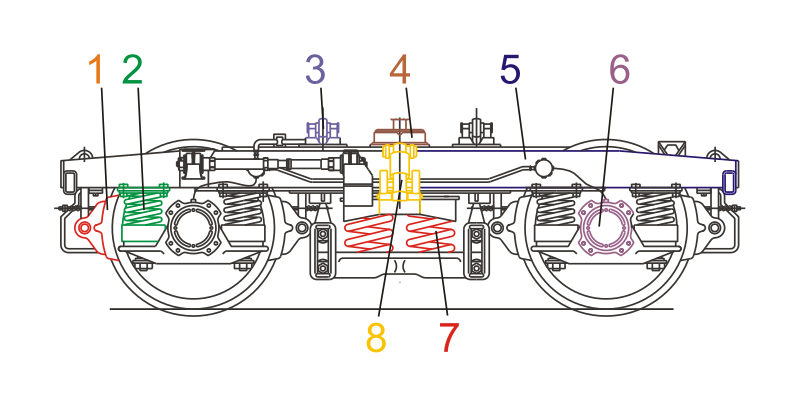
\includegraphics[width=15cm]{skryptkierownik-img/skryptkierownik-img027.png}
		\caption{Elementy budowy wózka, źródło: Wikipedia}
		\label{fig:wozek}
	\end{figure*}

\begin{enumerate}
	\item Klocek hamulcowy
	\item Pierwszy stopień usprężynowania
	\item Podparcia boczne
	\item Czop skrętu
	\item Rama wózka
	\item Maźnica
	\item Drugi stopień usprężynowania
	\item Tłumik drugiego stopnia usprężynowania
\end{enumerate}


\textbf{Pierwszy stopień usprężynowania} tworzy filtr mechaniczny tłumiący i amortyzujący drgania przenoszone z zestawu kołowego na ramę wózka. Elementami sprężystymi w tym rozwiązaniu są w starszych pojazdach sprężyny stalowe piórowe (resory), a w nowszych konstrukcjach sprężyny śrubowe naciskowe (pojedyncze lub wielokrotne), sprężyny gumowe lub sprężyny metalowo - gumowe. 

\textbf{Drugi stopień usprężynowania} tworzy filtr mechaniczny tłumiący i amortyzujący drgania przenoszone z wózka na nadwozie. Elementami sprężystymi w tym rozwiązaniu mogą być sprężyny śrubowe naciskowe lub dwufunkcyjne, sprężyny pneumatyczne, sprężyny metalowo - gumowe lub czasem sprężyny gumowe. 

Rodzaje sprężyn:
\begin{itemize}
	\item Sprężyny stalowe piórowe (\textbf{resory}) składają się z zespołu płaskich sprężyn zwanych piórami, które w części środkowej ujęte są opaską z zaciśniętym klinem. Pióra układane są na sobie w malejącej długości.
	\item \textbf{Sprężyny śrubowe} walcowe to odpowiednio nawinięte na gorąco pręty o przekroju kołowym. Sprężyny takie mogą być prawo lub lewoskrętne w zależności od kierunku ich nawijania. 
	W zależności od konstrukcji pojazdu mogą one pracować w wersji pojedynczej lub wielokrotnej. Wielokrotność polega na zastosowaniu współosiowo zamontowanych sprężyn przeciwnie skręconych (jedna sprężyna w drugiej). 
	Sprężyny śrubowe dzielą się na: sprężyny naciskowe, przenoszące tylko ruchy wzdłuż ich osi (stosowane w I i II st. usprężynowania) oraz sprężyny dwufunkcyjne typu \textbf{„flexicoil”}, czyli w tłumaczeniu „giętka spirala” przenoszące zarówno ruchy wzdłuż ich osi jak również ruchy poprzeczne (stosowane tylko w II st. usprężynowania). 
	Sprężyny dwufunkcyjne z jednej strony osadza się w gniazdach na podłużnicach ramy wózka, a z drugiej strony wspiera się na nich nadwozie. Ponieważ ten typ sprężyn przenosi zarówno ruchy pionowe jak i poziome nie ma potrzeby stosowania pośrednich elementów oparć nadwozia takich jak np. belek bujakowych, czy skrętowych, które umożliwiają realizację ruchów wózka w płaszczyźnie poziomej (obrotów), gdyż możliwość tych ruchów zapewnia już praca tych sprężyn w płaszczyźnie poziomej.
	\item sprężyny gumowe występują w postaci płyt płaskich lub kątowych, krążków, pierścieni stożkowych lub cylindrycznych. Mają dużą zdolność tłumienia drgań o wysokiej częstotliwości oraz dużą pojemność energetyczną względem masy.
	\item \textbf{sprężyny metalowo - gumowe} to elastyczne bloki w których skład wchodzi guma (sprężyna gumowa) odpowiednio zwulkanizowana zwulkanizowana z elementami metalowymi. Wulkanizacja w tym przypadku polega na trwałym powleczeniu (sklejeniu) gumą elementów metalowych. 
	W I stopniu usprężynowania najczęściej stosuje się sprężyny metalowo – gumowe typu pierścieniowego lub klinowego. 
	W tych pierwszych pomiędzy pierścieniami gumowymi znajdują się pasy gumy natomiast środkiem tego zespołu biegnie kolumna prowadząca zestaw kołowy. W rozwiązaniu klinowym, powszechnie stosowanym w nowych pojazdach trakcyjnych, sprężyna składa się z dwóch pakietów kątowych elementów gumowych przedzielonych kątowymi blaszkami.  
	\item  \textbf{sprężyny pneumatyczne} występują w wersjach membranowych lub półtoriodalnych. 
	W taborze pasażerskim najczęściej stosuje się sprężyny półtoriodalne - nie wymagają one stosowania belek skrętowych, gdyż mają właściwości umożliwiające dużą odkształcalność poprzeczną. Sprężyny półtoriodalne oparte są więc bezpośrednio na podłużnicach (belkach ostojnicowych) ramy wózka, a na nich spoczywa nadwozie pojazdu. Sprężyna pneumatyczna składa się z płyty mocującej, pierścienia, powłoki gumowej zwanej miechem sprężyny pneumatycznej wypełnionej sprężonym powietrzem oraz sprężyny dodatkowej. Sprężyna dodatkowa pełni funkcję awaryjną - w przypadku ubytku powietrza w miechu przejmuje obciążenia i umożliwia kontynuowanie jazdy z obniżoną prędkością. Usprężynowanie pneumatyczne wymaga układu zasilania pneumatycznego sprężonym powietrzem i sterowania. W układzie pneumatyki znajduje się zawór ważący, który utrzymuje stałą wysokość sprężyny dostosowując ciśnienie w miechu pneumatycznym do aktualnego obciążenia, reagując na zmiany ugięcia. 
	Sprężyny pneumatyczne naprzeciwległe są połączone pneumatycznie poprzez zawór wyrównawczy, który wyrównuje ciśnienia między sprężynami na wózku. W przypadku awarii jednego z miechów zawór ten wypuszcza też powietrze z miechu sprawnego, tak aby pudło z obydwu stron wparte było na sprężynie dodatkowej (awaryjnej) co zapewni wyrównanie nacisków nadwozia na wózek. 
	\end{itemize}

\textbf{Maźnica} zwana też łożyskiem głównym to element w którego skład wchodzą łożyska toczne (rzadziej ślizgowe) osadzone na czopach łożyskowych osi oraz kadłub (korpus) maźnicy, w którym te łożyska są osadzone. Kształt kadłuba maźnicy jest zależny oraz sposobu prowadzenia zestawu kołowego względem ramy wózka i metody mocowania odsprężynowania pierwszego stopnia.

Podział metod prowadzenia zestawu kołowego:
\begin{itemize}
\item \textbf{prowadzenie sztywne} 
Pierwszym opracowanym na początku istnienia kolei sposobem było sztywne prowadzenie zestawów kołowych do ramy w wyniku czego nie były one usprężynowane.
\begin{marginfigure}
	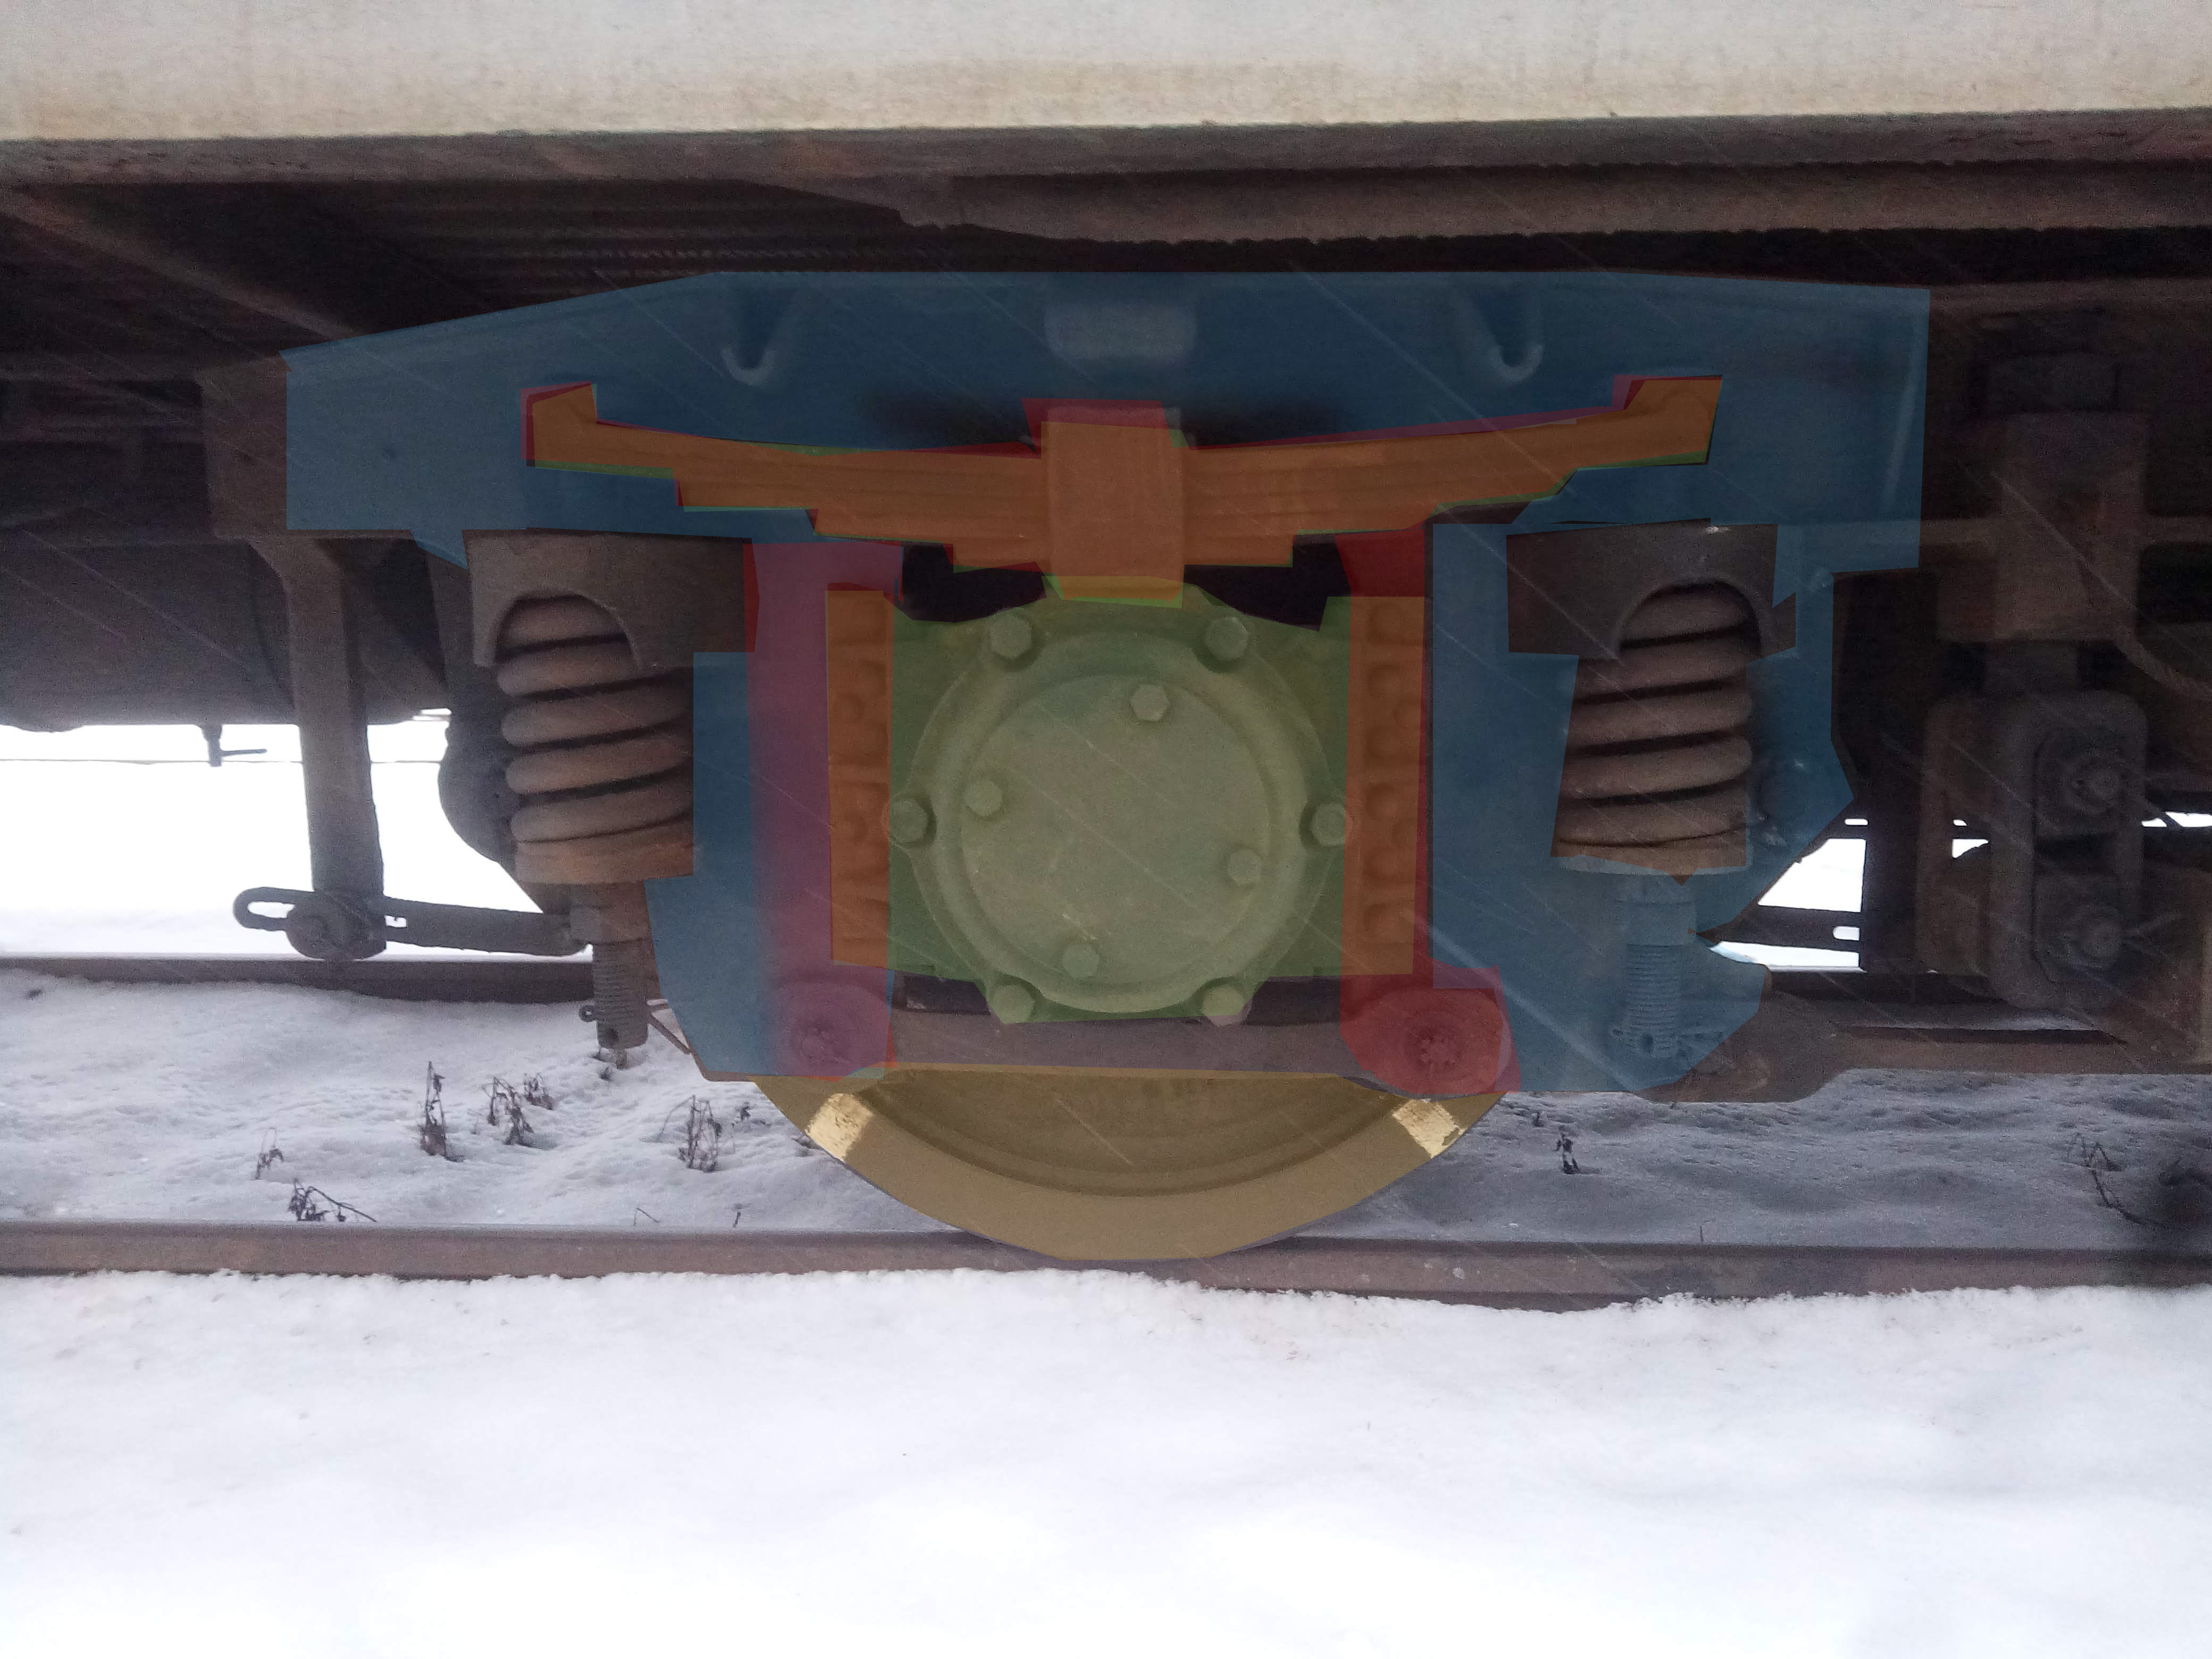
\includegraphics[width=5cm]{skryptkierownik-img/prowadzenie-zestawu-widlowe.jpg}
	\caption{Prowadzenie widłowe. Kolorem niebieskim oznaczona rama wózka.}
\end{marginfigure}
\item \textbf{prowadzenie widłowe} za pośrednictwem tak zwanych wideł maźniczych. Kadłub maźnicy posiada pionowe ścianki ze ślizgami (najczęściej miedzianymi). Ślizgi te te współpracują z wykładzinami wideł maźniczych ramy, które wykonane są ze stali. Prowadzenie widłowe może być jednostronne, dwustronne lub kątowe. 
\begin{marginfigure}
	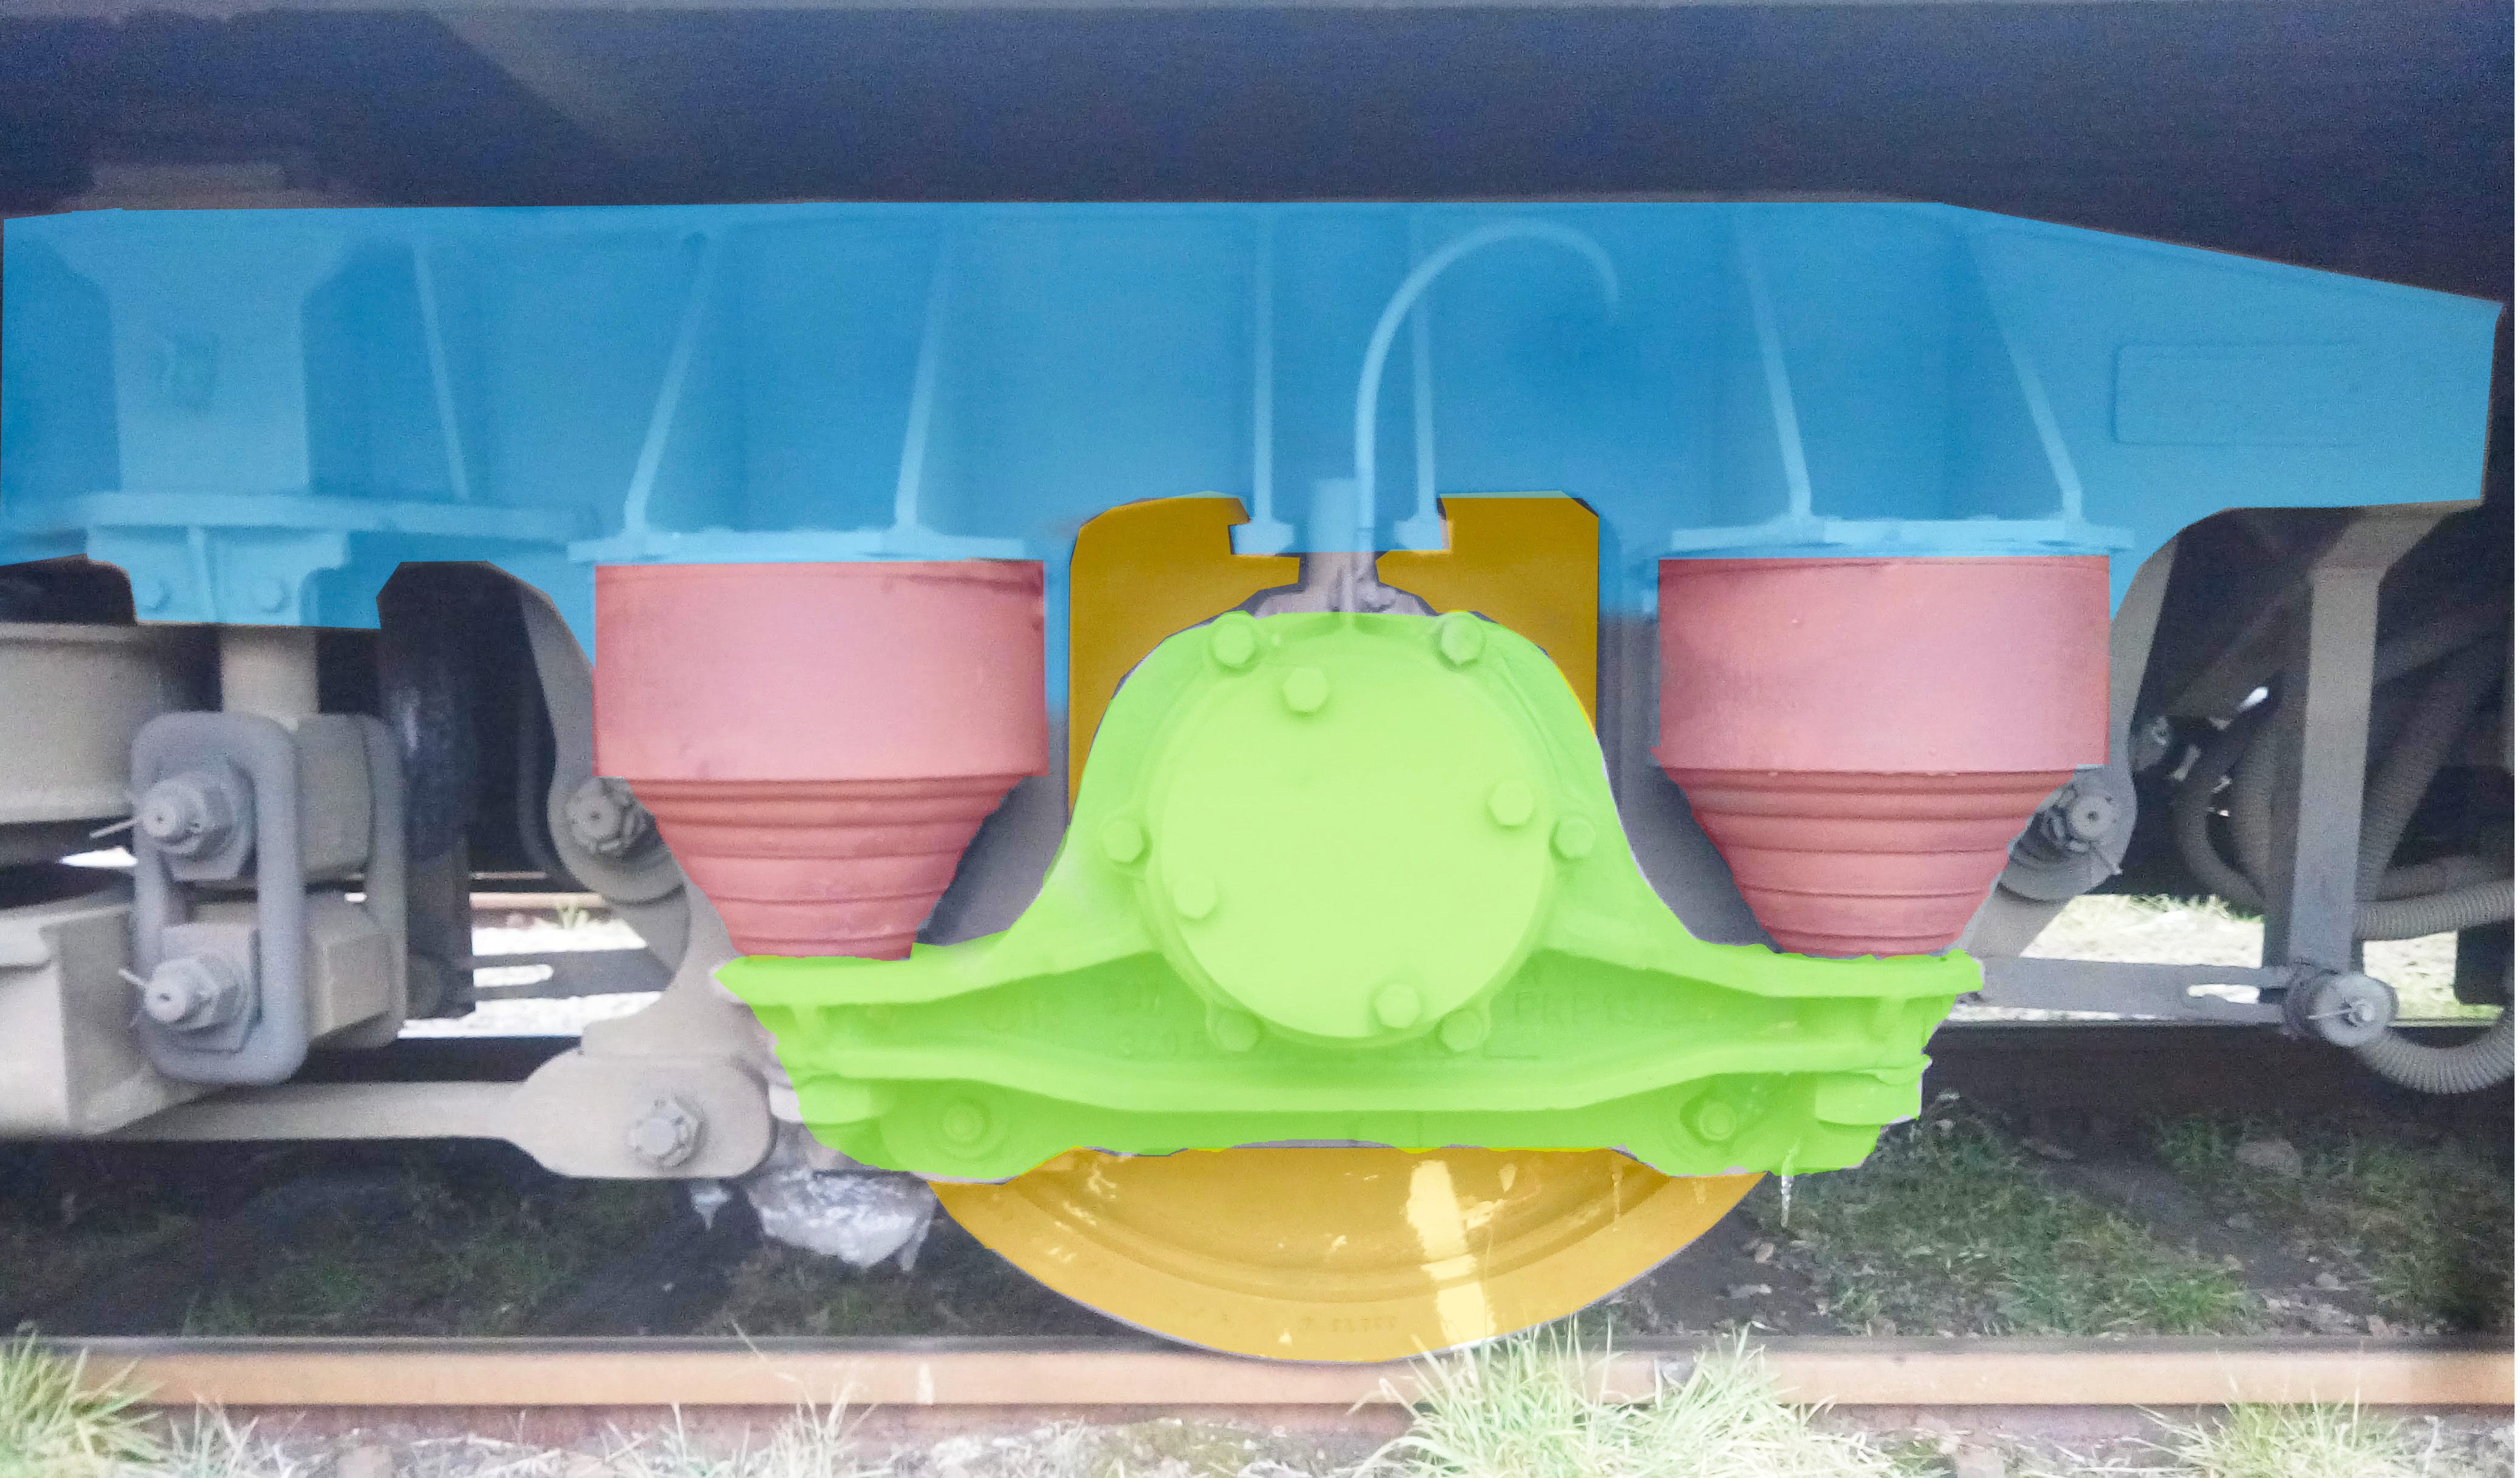
\includegraphics[width=5cm]{skryptkierownik-img/prowadzenie-zestawu-kolumnowe.jpg}
	\caption{Prowadzenie kolumnowe. Kolorem niebieskim oznaczona rama wózka, kolorem pomarańczowym zestaw kołowy, kolorem zielonym korpus maźnicy, zaś kolorem czerwonym kolumny gumowo-metalowe.}
\end{marginfigure} 
\item \textbf{prowadzenie kolumnowe} polegające na zastosowaniu sprężyn stalowych w których znajdują się kolumny prowadzące. Sprężyny i kolumny wsparte są w cylindrycznych gniazdach kadłuba maźnicy, a na ich drugim końcu oparta jest podłużnica ramy wózka (belka ostojnicowa). System ten daje dużą sztywność w płaszczyźnie poziomej, a zużycie cierne elementów prowadzenia jest niewielkie. 
\item \textbf{prowadzenie sprężyste-cięgnowe} (taśmowe) realizowane jest w płaszczyźnie poziomej, a płaskie cięgna sprężyste występują w układzie jedno lub dwustronnym. W prowadzeniu tym nie występuje zużycie ścierne. 
Omówione rozwiązanie występuje głównie w wózkach tocznych, gdyż zastosowane cięgna nie są przystosowane do przenoszenia dużych sił pociągowych i hamulcowych, jakie występują w pojazdach trakcyjnych. Wyjątek stanowią lekkie pojazdy trakcyjne, gdzie siły pociągowe są nieduże.
\begin{marginfigure}
	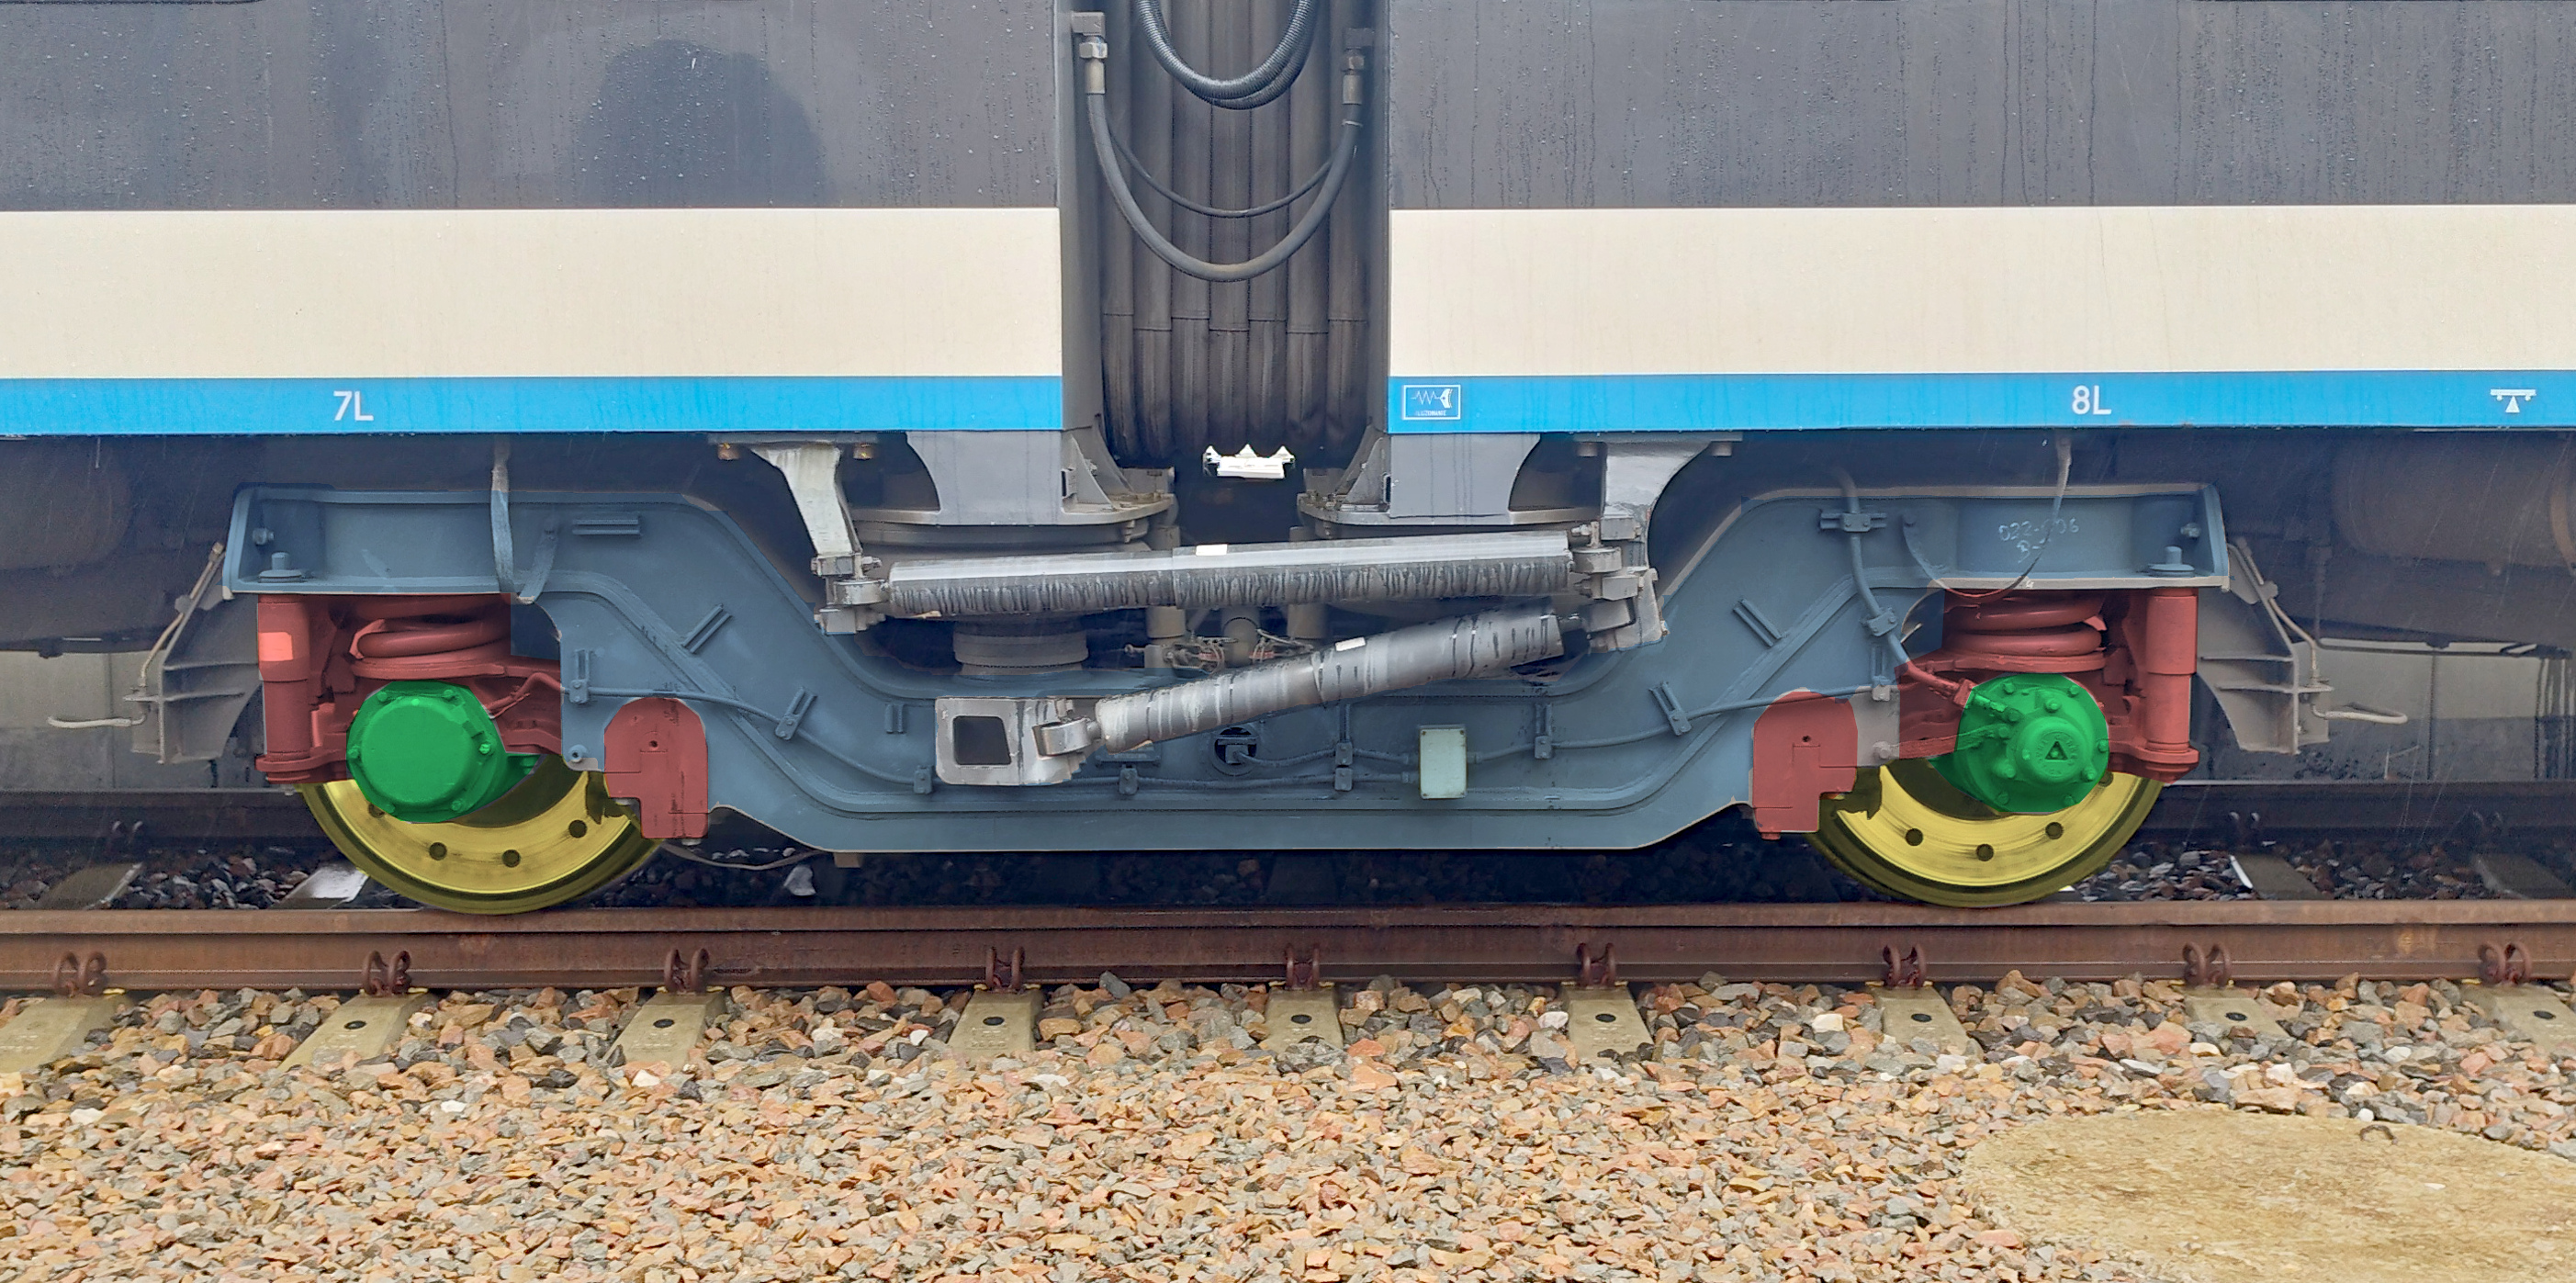
\includegraphics[width=5cm]{skryptkierownik-img/prowadzenie-zestawu-wahaczowe.jpg}
	\caption{Prowadzenie wahaczowe. Kolorem niebieskim oznaczona rama wózka, kolorem pomarańczowym zestaw kołowy. Kolorem czerwonym zaznaczono sprężynę pierwszego stopnia usprężynowania i wahacz.}
\end{marginfigure}
\item \textbf{prowadzenie wahaczowe} - ramię wahacza może być odlane ze staliwa wraz z cylindryczną częścią kadłuba maźnicy lub do niej przyspawane. Zastosowane w tym rozwiązaniu przeguby gumowo-metalowe powodują sprężyste prowadzenie w płaszczyźnie poziomej. Wahacz stanowi jednocześnie prowadzenie w kierunku poprzecznym. 
\end{itemize}

\textbf{Zestaw kołowy} składa się z \underline{osi} oraz \underline{dwóch kół jezdnych} osadzonych na niej w sposób trwały.
Wyróżnia się koła monoblokowe oraz obręczowane. 
Koła obręczowane składają się z \textbf{koła bosego} – piasty (które nabijane jest na podpiaście osi), \textbf{obręczy} i pierścienia \textbf{zaciskowego}. Koło bose może być ramienne lub tarczowe. Te pierwsze wykonywane są zawsze jako staliwne, natomiast koła tarczowe mogą być staliwne lub kute. 
Obręczowanie czyli proces mocowania obręczy na kole bosym polega na podgrzaniu obręczy przez rezystancję prądu elektrycznego do temperatury ponad 250 st. Celsjusza. Zgodnie z zasadą rozkurczania termicznego stali, obręcz zwiększa swoją średnicę w wyniku czego może być nabita na koło bose. W rowku obręczy specjalną walcarką osadza się natomiast pierścień zaciskowy. W procesie stygnięcia obręcz kurczy się i samoczynnie zaciska na kole bosym, a pierścień zaciskowy stanowi dodatkowe zabezpieczenie omówionego połączenia skurczowego.

Na obwodzie koła jezdnego, w miejscu połączenia obręczy z kołem bosym maluje się promieniście białe paski w celu stwierdzenia ewentualnego przesunięcia obręczy. Paski powinny mieć szerokość 30mm, oraz rozmieszczone co 90 stopni na obwodzie koła. \textbf{Poluzowanie} się obręczy, czy też jej \textbf{pęknięcie} jest elementem zagrażającym bezpieczeństwu dlatego konieczne są częste kontrole współpracy tych elementów poprzez uderzanie młotkiem w obręcz i ocenę odgłosu (wykonuje to rewident taboru). 

Koła \textbf{monoblokowe} różnią się od obręczowych tym, że stanowią jedną całość, to znaczy piasta oraz obręcz, zwana w kołach monoblokowych wieńcem, są wykonane z jednego elementu stalowego w związku z czym nie ma możliwości wymiany obręczy po jej zużyciu. Konieczna jest wymiana całego koła. Rozwiązanie to poprawia znacząco bezpieczeństwo jazdy, gdyż nie ma możliwości poluzowania się obręczy. Na obwodzie koła monoblokowego wytłoczony jest rowek wskazujący graniczne zużycie powierzchni tocznej. Rowek ten musi być widoczny w całośći.

Połączenie wózka z pudłem pojazdu zapewnia gniazdo czopa skrętu, zabudowane w górnej części wózka i czop skrętu w pudle. Czop skrętu jest osią obrotu wózka - realizuje jego obroty w płaszczyźnie poziomej zgodnie z kierunkiem torów.  

\section{Urządzenia pociągowo-zderzne}

Urządzenia pociągowo - zderzne w taborze kolejowym służą do mechanicznego połączenia poprzez sprzęgi pojazdów kolejowych ze sobą, przenoszenia sił pociągowych oraz do łagodzenia sił wzdłużnych wynikających z nabiegania pojazdów na siebie podczas jazdy przy jednoczesnym pochłanianiu części energii powstałej na skutek tego nabiegania. Dzięki powyższym możliwe jest uformowanie składu pociągu z zapewnieniem bezpieczeństwa oraz płynnej i komfortowej jazdy.

Pod względem rodzajów urządzeń pociągowo - zderznych rozróżnia się te, gdzie urządzenia sprzęgowe montowane są niezależnie od zderzakowych oraz takie, gdzie stanowią one zintegrowany element.
W pierwszym przypadku na czołach ostoi pojazdów zabudowuje się w osi wzdłużnej pojazdu urządzenie cięgłowe ze sprzęgiem śrubowym, a po obu jego stronach zabudowywane są urządzenia zderzakowe. W drugim przypadku w ostoi zabudowuje się sprzęgi samoczynne, czyli urządzenia w których zintegrowana jest funkcja cięgłowa, sprzęgająca i zderzakowa.

Sprzęgi typu Scharfenberga realizują jednocześnie połączenie mechaniczne, elektryczne i pneumatyczne pojazdów kolejowych. Wykorzystywane są najczęściej do łączenia w trakcję ukrotnioną jednostek trakcyjnych pasażerskich (EZT i SZT).

Zaletą sprzęgów typu Scharfenberga jest ich samoczynność. Umożliwiają one sprzęganie jednostek bez konieczności użycia żadnych dodatkowych narzędzi, urządzeń, ani tym bardziej personelu. Każdy sprzęg omawianego typu składa się z wypustu stożkowego i gniazda dokładnie odpowiadającemu kształtem takiemu wypustowi.
Dojeżdżając z prędkością nie przekraczającą 5km/h jednostką do drugiej jednostki następuje zetknięcie sprzęgów. Łącznik jednego sprzęgu wchodzi w gniazdo drugiego (sercówkę), a łącznik drugiego wchodzi w sercówkę pierwszego. Łączniki samoczynnie zaczepiają się w sercówkach poprzez mechanizm zaczepowy. Ponad głowicą sprzęgu lub po jej bokach znajduje się tak zwana klawiatura, która zapewnia elektryczne połączenie między jednostkami.

W przypadku konieczności sprzęgnięcia pojazdu wyposażonego w sprzęg typu Scharfenberga z pojazdem, który posiada klasyczny sprzęg śrubowy stosuje się specjalne adaptery sprzęgu zwane też półsprzegami, które z jednej strony posiadają
zespół sprzęgu automatycznego, a z drugiej strony zakończone są w sposób umożliwiający założenie na hak cięgłowy.

\section{Odbierak pradu}
Odbieraki prądu pojazdów szynowych to aparaty służące do ruchomego połączenia stykowego sieci trakcyjnej z elektrycznym obwodem głównym pojazdu trakcyjnego. Rozróżnia się odbieraki górne, zwane również pantografami (ang. pantograph), czyli te współpracujące z siecią trakcyjną napowietrzną oraz odbieraki dolne do poboru energii z tak zwanej trzeciej szyny prądowej, która prowadzona jest równolegle do szyn toru na ich poziomie. 
Pantografy są najpopularniejsze w kolejnictwie oraz komunikacji tramwajowej. Odbieraki dolne, używane są głównie na liniach metra oraz szybkich kolei miejskich, gdzie do infrastruktury nie mają dostępu osoby postronne. 

\begin{marginfigure}
	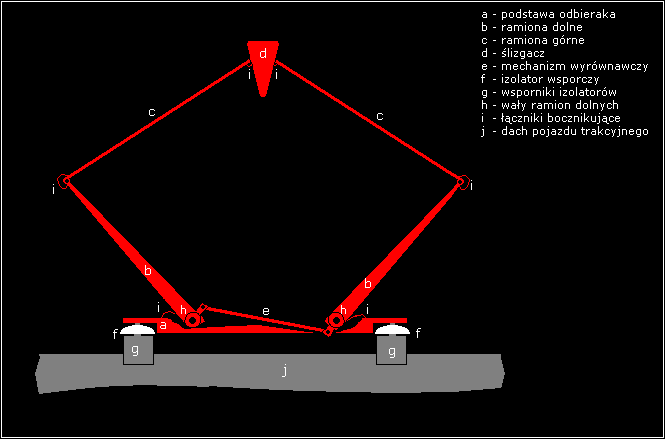
\includegraphics[width=6cm]{skryptkierownik-img/kolodbierakschem1.png}
	\caption{Odbierak o konstrukcji ramy - nożycowej. Źródło: www.transportszynowy.pl}
	\label{fig:pantograf1}
\end{marginfigure}

Odbieraki prądu górne składają się z trzech głównych elementów: podstawy z napędem, ramy przegubowej i ślizgacza. 
\begin{itemize}
	\item \textbf{Podstawa} - to nieruchomy element konstrukcji pantografu, do której przymocowane są części ruchome i układ napędowy. Podstawa jest przymocowana do dachu pojazdu trakcyjnego za pośrednictwem izolatorów wsporczych, izolujących elektrycznie pantograf od pudła pojazdu trakcyjnego. Układ napędowy służy do podnoszenia odbieraka i utrzymywania go w pozycji podniesionej, zapewniając jednocześnie prawidłową siłę docisku do przewodu jezdnego oraz jego opuszczania z zapewnieniem wymaganej siły opuszczającej, a w pozycji dolnej siły utrzymującej go w położeniu złożonym. 

	\item Ruchoma \textbf{rama} przegubowa składa się z układu ramion połączonych przegubowo. Układ ten służy do regulacji pionowej wysokości ślizgacza oraz zapewnia jego docisk na skutek działania układu napędowego. 
	
	
	\item \textbf{Ślizgacz} to część realizująca bezpośredni styk z przewodem jezdnym sieci trakcyjnej. Ślizgacz montowany jest do ramy przegubowej (ramion) elastycznie poprzez zastosowanie np. małego pantografu lub układu elementów sprężystych. Rozróżnia się ślizgacze pojedyncze, w których nakładki ślizgowe powiązane są ze sobą w sposób sztywny oraz ślizgacze bliźniacze w których zastosowane są dwa zestawy nakładek ślizgowych niezależnych lub powiązanych elastycznie. 
\end{itemize}
\begin{marginfigure}
	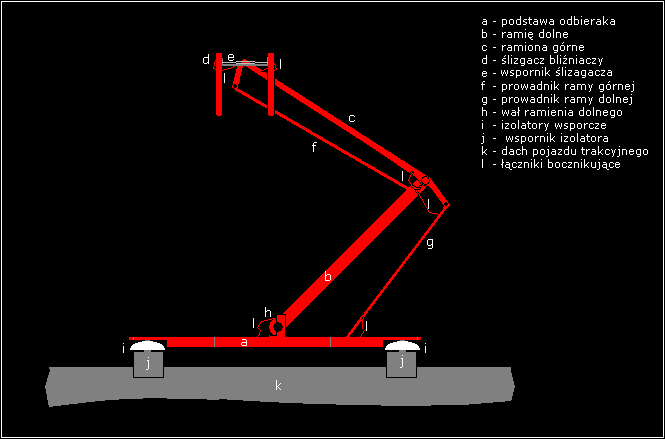
\includegraphics[width=6cm]{skryptkierownik-img/kolodbierakschem2.png}
	\caption{Odbierak o konstrukcji ramy - pantografowej. Źródło: www.transportszynowy.pl}
	\label{fig:pantograf2}
\end{marginfigure}	
Nakładki ślizgowe to elementy bezpośrednio stykające się z przewodem jezdnym. Wykonane są ze sprasowanego grafitu (węgla metalizowanego, węgla twardego). Parametry nakładek muszą być odporne na nagrzewanie i spełniać wymagania dotyczące obciążalności prądowej. W przypadku stosowania nakładek miedzianych ślizgacz pokrywa się warstwą smaru grafitowego, który zmniejsza rezystancję i tarcie, a jednocześnie jest źródłem bardzo widocznych zabrudzeń pojazdów. 
Po zewnętrznych stronach ślizgaczy znajdują się nabieżniki, które służą do wprowadzania przewodu jezdnego dochodzącego z boku na część roboczą ślizgacza. 

Pod względem elektrycznym odbierak prądu musi zapewniać prawidłowy przepływ energii elektrycznej przez swoją konstrukcję. Przegubowa budowa pantografów stwarza szczególnie właśnie w rejonie przegubów miejsca zakłóceń dla toru prądowego biegnącego z przewodu jezdnego, przez ślizgacz, ramę przegubową, do zacisku wyjściowego znajdującego się w ramie podstawy. Z tego powodu na przegubach stosuje się tak zwane łączniki bocznikujące. Są to elementy wykonane z giętkiej linki lub taśmy miedzianej, które poprawiają przepływ energii elektrycznej przez odbierak. Łączniki bocznikujące występują na łączeniach pomiędzy ślizgaczem, a ramionami górnymi, na przegubie ramion górnych z dolnymi oraz pomiędzy ramionami dolnymi, a ramą podstawy. 

Podniesienie odbieraka prądu do pozycji roboczej (styk z przewodem jezdnym) umożliwia pełne uruchomienie pojazdu trakcyjnego dzięki podłączeniu go do zasilania. W pojazdach kolejowych do podnoszenia odbieraków prądu wykorzystywany jest napęd pneumatyczny, znajdujący się w podstawie. Jednak, aby on zadziałał potrzebne jest sprężone powietrze nabite przez sprężarkę. Do uruchomienia sprężarki głównej w pojazdach potrzebne jest napięcie sieciowe, którego przy opuszczonym pantografie w pojeździe nie ma. Z tego też powodu w celu podniesienia odbieraków prądu przy uruchamianiu pojazdu w przypadku braku ciśnienia w zbiorniku głównym, pantografy posiadają niezależną sprężarkę ze zbiornikiem, która zasilana jest z baterii akumulatorów. Najpierw załącza się ją, a po nabiciu przez nią powietrza, maszynista podnosi pantograf. Po zasileniu pojazdu napięciem sieciowym, układ pneumatyczny pantografów zostaje przełączony na zasilanie ze sprężarki głównej (głównego układu pneumatycznego). 

Przewody jezdne sieci trakcyjnej kolejowej zawieszane są na wysokości od minimalnej 4900mm do maksymalnej 6200mm ponad główkę szyny. W takim zakresie wysokości ślizgacz musi mieć zapewniony prawidłowy docisk do przewodu jezdnego.

Jazda z podniesionym tylnym odbierakiem jest najbardziej optymalna, gdyż w przypadku złamania podniesionego odbieraka prądu nie opadnie on na pantograf złożony przez co będzie możliwa jazda awaryjna na pantografie przednim. Poza tym następuje zużycie nakładek ślizgowych tylko jednego slizgacza. Drugi pantograf pełni funkcję rezerwową. 

\section{Warunki techniczne jakim powinien odpowiadać tabor w składzie pociągu}

Wagony które nie posiadają blokady drzwi wejściowych, nie mogą być dopuszczone do ruchu międzynarodowego.

Przestrzeń berneńska (również prostokąt berneński) – wolna przestrzeń przed czołem pojazdu szynowego, w której nie mogą znajdować się żadne części taboru, stanowiąca bezpieczne miejsce dla pracownika spinającego wagony. Przestrzeń ta powinna być wolna od części stałych. W związku z tym wymaganiem części składowe mechanizmu sprzęgającego powinny znajdować się w położeniu bocznym względem jego linii środkowej.

W przestrzeni tej mogą znajdować się kable połączeniowe i węże elastyczne, jak również elastyczne odkształcalne elementy przejść międzywagonowych. Pod zderzakami nie powinny znajdować się żadne urządzenia, które utrudniałyby dostęp do omawianej przestrzeni. 
Części sprzęgów śrubowych, hamulcowych i innych sprzęgów nie mogą zwisać niżej niż \underline{140mm} powyżej główki szyny.

Powierzchnia toczna koła nie może być miejscami wgnieciona, mieć płaskich miejsc i nalepów \textbf{dłuższych} niż \underline{60mm}, oraz o \textbf{głębokości lub wysokości} do \underline{1mm}. Powierzchnia toczna nie może mieć żadnych rys na przejściu z powierzchni tocznej na czołową. Uszkodzenia na powierzchni tocznej (wyłupania, dziury, złuszczenia, odpryski) nie mogą być dłuższe niż 60 mm. W razie powstania wyżej opisanych nalepów hamulec zespolony należy wyłączyć. Wagon okleić nalepkami według wzoru $R^{1}$ („Hamulec niezdatny do użytku”) i \textbf{M} („Do zbadania”), na których należy zaznaczyć : „Nalepy na powierzchni tocznej”.
Koła obręczowane z wytoczonym rowkiem na zewnętrznej powierzchni czołowej obręczy, pokazującym zużycie, są niedozwolone.
W kołach monoblokowych minimalna grubość wieńców kół musi być oznaczona za pomocą \textbf{rowka} wytoczonego na zewnętrznej powierzchni czołowej koła. Rowek musi być stale w całości widoczny.
Obręcze nie mogą mieć żadnego pęknięcia oraz żadnej rysy poprzecznej ani podłużnej. W kole obręczowanym - obręcz nie może być luźna.
Obręcz należy uważać za luźną, jeśli wykazuje co najmniej jedna z niżej wymienionych oznak:

\begin{itemize}
	\item obrót obręczy na kole bosym w płaszczyźnie koła, stwierdzony przez nie pokrywanie się znaków kontrolnych na kole bosym i obręczy.
	\item nieczysty dźwięk przy uderzeniu młotkiem
	\item luźne osadzenie pierścienia zaciskowego,
	\item występowanie rdzy na więcej niż 1/3 obwodu między obręczą a kołem bosym
	\item obręcz nie może wykazywać żadnych śladów bocznego przesunięcia (boczne przesuniecie może zaistnieć tylko wtedy, gdy brak pierścienia zaciskowego, jest luźny, złamany lub widocznie zniekształcony).
	\item pierścień zaciskowy nie może posiadać żadnej rysy. Jeśli dla zabezpieczenia pierścienia zaciskowego przewidziany jest klin zabezpieczający, nie może go brakować.
\end{itemize}

Koło nie może wykazywać żadnych śladów przesunięcia na osi zestawu. Występowanie oleju między osią zestawu kołowego i piastą koła nie jest dowodem, że koło przesunęło się na osi; przesunięcie takie musi być udowodnione.
Piasta koła nie może mieć żadnej rysy. Koło monoblokowe lub tarcza koła nie mogą wykazywać żadnych śladów usuwania usterek spawaniem oraz żadnej rysy.

Oś zestawu kołowego nie może mieć żadnych śladów rys ani śladów naprawiania uszkodzeń przez spawanie, być zgięta, mieć żadnych wytartych miejsc z ostrymi krawędziami, wykazywać żadnych wytartych miejsc o głębokości większej niż 1 mm. Cięgła hamulcowe lub inne części nie mogą trzeć o oś zestawu. Uszkodzone części należy zdemontować lub wysoko umocować tak, aby ich tarcie o oś było niemożliwe. W tym przypadku, a także gdy oś zestawu ma wytarcia mniejsze niż podano wyżej, wagon należy okartkować nalepkami według wzoru \textbf{M} („Do zbadania”), na których należy zaznaczyć „zestaw kołowy”.

W razie podejrzenia termicznego wpływu hamulca na koła monoblokowe objawiające się przez:
\begin{itemize}
	\item świeże ślady spalenia farby na przejściu wieńca w tarczę lub świeże ślady utlenienia wieńca koła lub
	\item nadpalone wstawki hamulcowe lub
	\item uszkodzona powierzchnia toczna z nalepami
\end{itemize}
należy dokonać pomiaru rozstawu kół między wewnętrznymi czołowymi powierzchniami wieńców kół.
 
Łożyska zestawu kołowego nie mogą być tak uszkodzone, aby wyciekał z nich środek smarny lub mógł do ich wnętrza dostawać się kurz i woda. Występy prowadne maźnic muszą w każdym położeniu maźnicy obejmować prowadniki wideł lub odpowiednie części wózków. Łożysko nie może być tak gorące, aby nie można było go dotknąć zewnętrzną powierzchnią dłoni. Łożyska mogą być smarowane i naprawiane przez przedsiębiorstwo kolejowe właściciela. W razie uszkodzenia musi być zawsze wbudowany nowy zestaw kołowy.

Sprężyny śrubowe (spiralne) i piórowe nie mogą być złamane, zaś sprężyny piórowe również przesunięte wzdłuż w opasce o więcej niż 10mm. Wszystkie sprężyny muszą być prawidłowo osadzone w swoich mocowaniach. Tłumiki nie mogą być luźne, oraz posiadać oznak uszkodzeń takich jak wycieki, nieszczelność. wieszaki belek bujakowych i prowadniki zestawów kołowych nie mogą być zgięte , pęknięte, lub złamane,a ich połączenia luźne. Połączenia spawane poprzecznic i podłużnic nie mogą mieć rys. W tych elementch konstrukcyjnych nie mogą również występować żadne nadpęknięcia wychodzące od spoin spawalniczych.
Złamania, uszkodzenia i nadpęknięcia podłużnic, poprzecznic, ram wózków, wsporników belki bujakowej oraz połączeń wózków mogą być naprawiane przez spawanie tylko przez właściciela wagonu.

W każdym wagonie musi być zgodnie z kartą UIC 564-2 przynajmniej jedna gaśnica. W wagonach sypialnych i restauracyjnych muszą być po dwie gaśnice,
Gaśnice muszą być stale zdatne do użytku i dostępne dla podróżnych. 

Wszystkie drzwi wejściowe muszą mieć urządzenia blokujące zapobiegające niezamierzonemu otwarciu drzwi wejściowych w czasie jazdy. Drzwi wagonowe, ich urządzenia prowadne i zamykające oraz elektropneumatyczne urządzenia zamykania drzwi i urządzenia blokowania drzwi nie powinny wykazywać żadnych usterek, które w znacznym stopniu ograniczają użycie wagonu, względnie zagrażają bezpieczeństwu uchu.

\subsection{Oznakowanie i symbole na taborze}

Każdy wagon musi być oznaczony numerem EVN oraz symbolem opisującym cechy techniczne wagonu albo typ i numer serii pojazdu trakcyjnego. Dodatkowo wagon powinien posiadać znaki RIV, RIC, TEN lub MC.

\textbf{Europejski numer pojazdu} (ang. European Vehicle Number, EVN) to numer składający się z 12 cyfr zawierający informacje o charakterystyce technicznej pojazdu kolejowego. 
Numer ten zapisujemy w kilku blokach z których pierwszy (dwucyfrowy) oznacza kod interoperacyjności - przy czym jeśli pierwsza cyfra to 9, jest to pojazd trakcyjny, zaś druga cyfra tego bloku opisuje sposób napędu i konstrukcji (4 oznacza EZT małej prędkości). Kolejne dwie cyfry to kod kraju (Polska to 51), kolejny, jednocyfrowy blok oznacza przeznaczenie pojazdu (cyfra 2 oznacza zespół trakcyjny). W kolejnym bloku opisane są sposób zasilania i moc pojazdu w MW. Pozostałe cyfry oznaczają numer kolejny pojazdu, zaś ostatnia cyfra jest cyfrą samokontroli.

Umowy RIV i RIC zostały zawarte w 1922 r. jako porozumienia międzynarodowe pomiędzy przedsiębiorstwami przewozowymi. Umowa RIV została rozwiązana 1 lipca 2006 r. Jednocześnie za  następcę tej umowy w obrocie międzynarodowym uznać można Ogólną umowę o użytkowaniu wagonów towarowych (GCU, AVV).

Podstawowymi zadaniem ww. umów jest uznawanie za dopuszczone do eksploatacji pojazdów kolejowych przez krajowe organy regulacji rynku kolejowego. Porozumienia te określają warunki, których spełnienie uzależnia możliwość wymiany pojazdów pomiędzy sygnatariuszami porozumienia. Spełnienie wymagań wskazanych w umowach jest stwierdzane poprzez nadanie pojazdom odpowiednio oznaczenia RIV lub RIC.
\begin{marginfigure}
	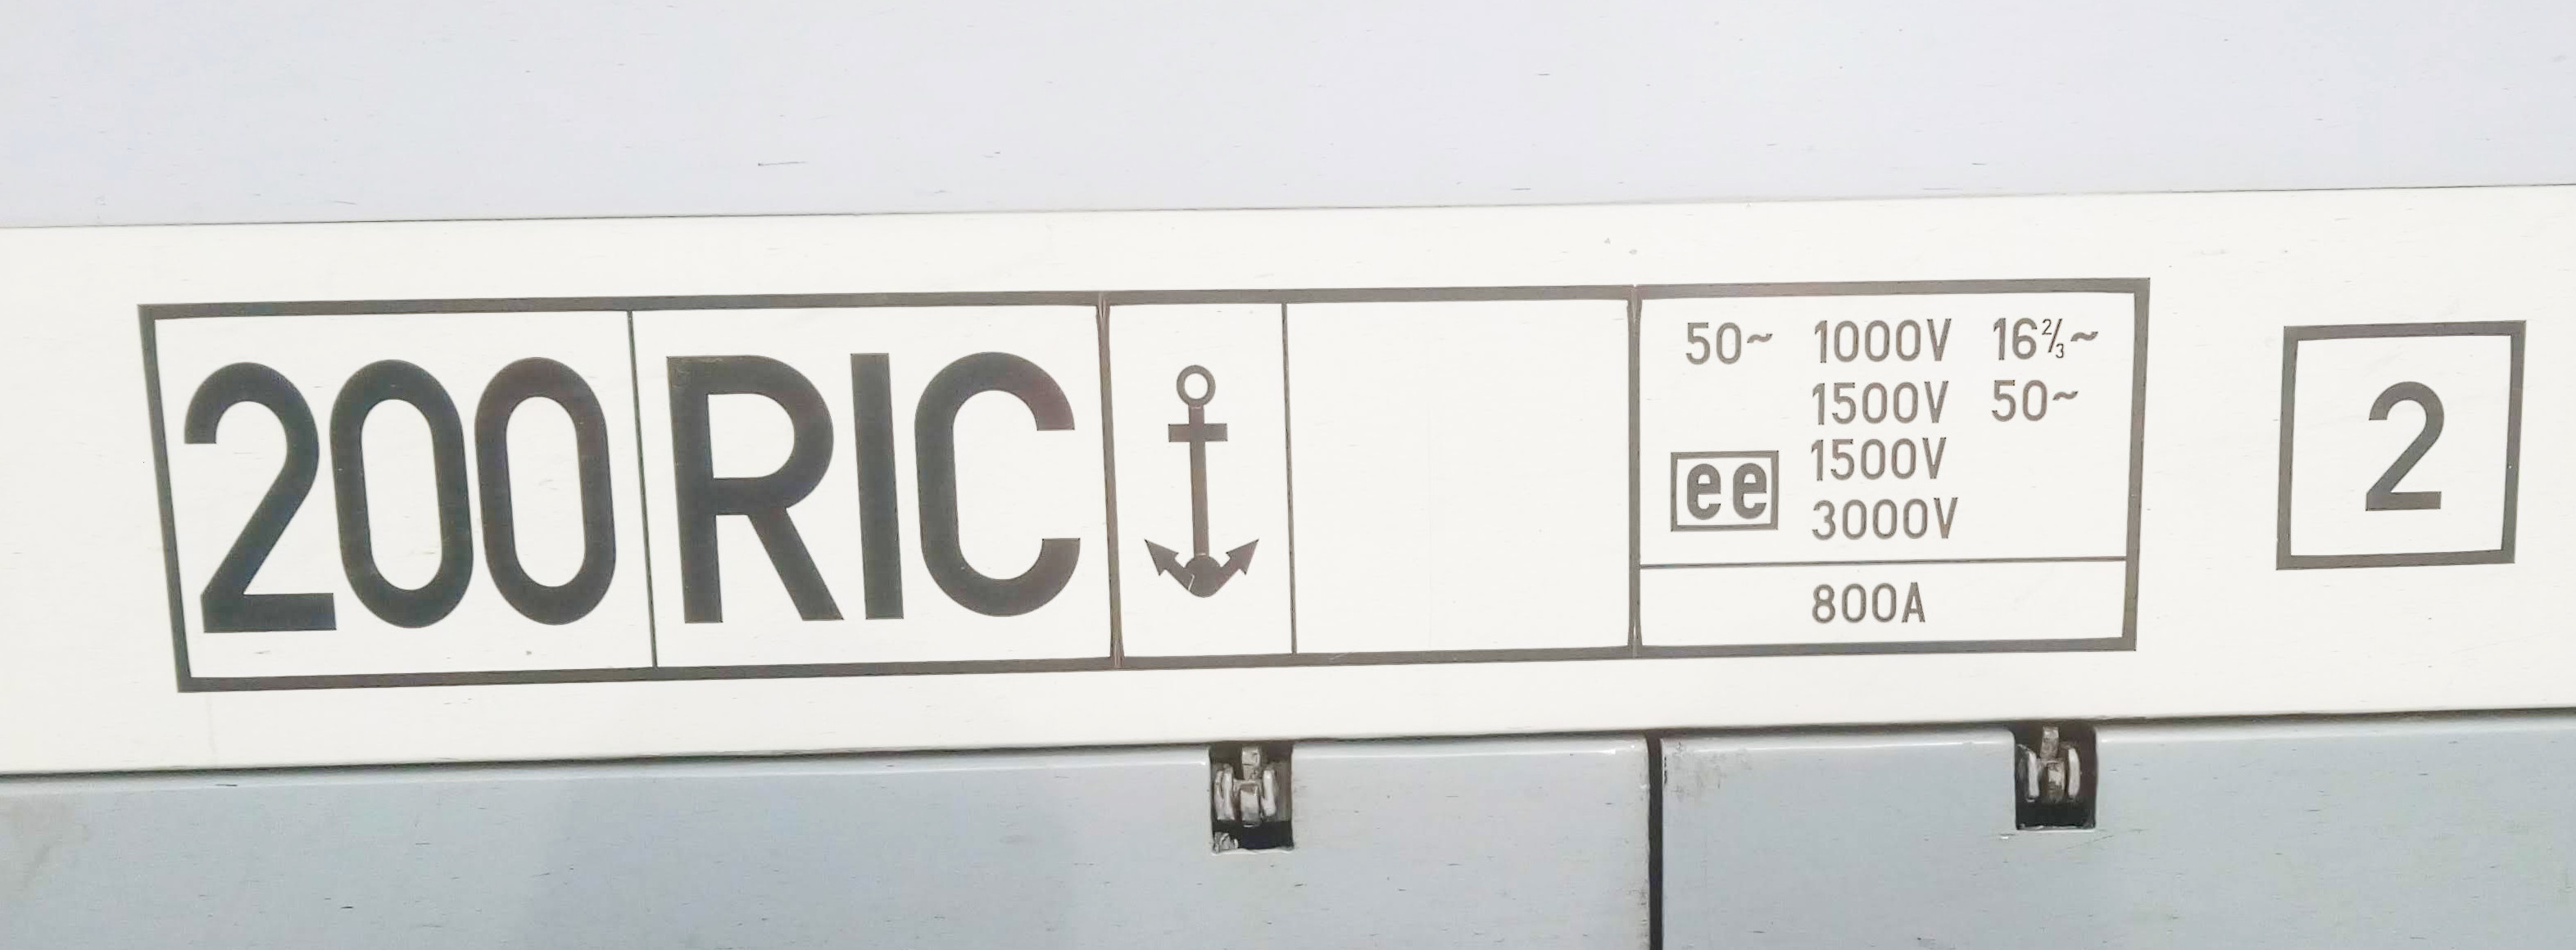
\includegraphics[width=6cm]{skryptkierownik-img/znak-ric.jpg}
	\caption{Znak RIC na wagonie PKP Intercity}
	\label{fig:pantograf2}
\end{marginfigure}

\textbf{RIV} - umowa międzynarodowa Regolamento Internazionale Veicoli. Były to przepisy o wzajemnym użytkowaniu wagonów towarowych w komunikacji międzynarodowej. Zostały zastąpione przez GCU (General Contract of Use for Wagons, czyli ogólna umowa o użytkowaniu wagonów towarowych).

\textbf{RIC} - umowa międzynarodowa Regolamento Internazionale Carozzi. Były to przepisy o wzajemnym użytkowaniu wagonów osobowych i bagażowych w komunikacji międzynarodowej.

\textbf{SMGS} - Umowa o międzynarodowej komunikacji towarowej obowiązująca w krajach Europy wschodniej (kraje dawnego ZSRR), Dalekiego Wschodu (Chiny, Korea, Wietnam, etc.) 

\textbf{Znak MC} - wagon spełniający przepisy PPW - określające normy i wymagania dla przewozów na podstawie umowy SMGS. 


\section{Wyłączanie taboru z eksploatacji}

\textbf{Przeglądy} – zabiegi zapobiegawcze wykonywane na sprawnym technicznie pojeździe w celu sprawdzenia zgodności stanu technicznego pojazdu trakcyjnego z obowiązującymi wymogami bezpieczeństwa ruchu kolejowego i eksploatacyjnymi określonym m.in. w \textbf{Dokumentacji Systemu Utrzymania} (DSU).

\textbf{Naprawy} - czynności mające na celu doprowadzenie wyeksploatowanego (zużytego) lub uszkodzonego pojazdu trakcyjnego wyłączonego z ruchu, jego zespołu, podzespołu, elementu, obwodu lub układu do wymaganego przepisami technicznymi stanu pełnej sprawności wg wymogów (DSU) umożliwiającego dalszą bezpieczną eksploatację.

\textbf{Poziom utrzymania pojazdu kolejowego} – zestawienie czynności utrzymaniowych wykonywanych dla danego pojazdu kolejowego określone zakresem tych prac;

\textbf{Modernizacja pojazdu kolejowego} – prace modyfikacyjne w pojeździe kolejowym, które zmieniają przeznaczenie pojazdu lub poprawiają jego ogólne osiągi techniczne, a w szczególności: zmianę charakterystyki trakcyjnej, prędkości maksymalnej, mocy, zdolności do zasilania w różnych systemach;
Wyłączenie pojazdu trakcyjnego z eksploatacji winno nastąpić gdy pojazd nie spełnia wymagań formalnych lub technicznych i nie zapewnia odpowiedniego poziomu bezpiecznej eksploatacji.

Pojazd kolejowy nalezy wyłączyć z eksploatacji, jeżeli:
\begin{enumerate}
	\item jego świadectwo sprawności technicznej utraciło ważność,
	\item kiedy wymaga wykonania przeglądu poziomu 1,2, lub 3.
	\item w razie dalszej eksploatacji zachodzi uzasadnione prawdopodobieństwo
	przekroczenia dopuszczalnego czasokresu bądź przebiegu do następnego
	przeglądu poziomu utrzymania 1, 2 lub poziomu 3 - zgodnie z obowiązującą
	dla danej serii pojazdu trakcyjnego dokumentacją systemu utrzymania.
	\item wymaga wykonania naprawy okresowej lub bieżącej, awaryjnej, bądź usunięcia
	usterek i innych nieprawidłowości - w szczególności, gdy uczestniczył w zdarzeniu kolejowym, bądź w książce pokładowej pojazdu kolejowego z napędem znajdują się adnotacje o nieprawidłowościach istotnych dla bezpieczeństwa ruchu kolejowego,
	\marginnote{Wszystkie oznaczenia takie jak EVN, masy służbowe, hamujące, oznaczenia nastawienia hamulca, etc. muszą być czytelne.}
	\item znaki i napisy na pojeździe trakcyjnym są nieczytelne lub niezgodne z obowiązującymi przepisami,
	\item pobieżne, zewnętrzne oględziny pojazdu trakcyjnego lub działanie zespołów, podzespołów i elementów mogą wskazywać na uszkodzenia lub inne, istotne nieprawidłowości,
	\item wynika to z wewnętrznych poleceń kierownictwa komórki organizacyjnej Spółki
\end{enumerate}

Dopuszczenie pojazdu trakcyjnego Spółki do eksploatacji może odbyć się wyłącznie po spełnieniu wymagań formalnych i technicznych oraz po wykonaniu zabiegów utrzymaniowych określonych w DSU, gdy pojazd jest sprawny technicznie i zapewnia jego bezpieczną eksploatację.

Dopuszczenie do eksploatacji pojazdu trakcyjnego, uprzednio wyłączonego z eksploatacji, może nastąpić, jeżeli pojazd posiada:
\begin{itemize}
	\item świadectwo dopuszczenia typu pojazdu do eksploatacji,
	\item ważne świadectwo sprawności technicznej,
	\item udokumentowany przegląd i naprawę właściwego poziomu utrzymania 1, 2 i 3 oraz gdy dopuszczenie do eksploatacji nie spowoduje przekroczenia obowiązującego resursu,
	\item została wykonana naprawa bieżąca, awaryjna, bądź usunięto usterki i inne nieprawidłowości - o ile zachodziła taka potrzeba,
	\item w książce pokładowej pojazdu kolejowego z napędem pracownik zamieścił adnotację o wykonanej naprawie bieżącej lub awaryjnej o zgodności wyników pomiarów z wymaganiami, lub o przeprowadzeniu przeglądu o odpowiednim poziomie utrzymania,
	\item znaki i napisy na pojeździe trakcyjnym są czytelne oraz zgodne z obowiązującymi przepisami, 
	\item ważne świadectwo sprawności technicznej pojazdu umieszczone w kabinie maszynisty,
	\item pozytywny wynik oględzin pojazdu trakcyjnego.
\end{itemize}
Fakt dopuszczenia pojazdu trakcyjnego do eksploatacji należy odnotować w książce pokładowej pojazdu kolejowego z napędem zapisem o treści:
„dopuszczam pojazd trakcyjny serii ... nr ... do eksploatacji", który winien być potwierdzony podpisem, datą, godziną, nazwą miejscowości i stemplem imiennym. Po dokonaniu wpisu dotyczącego dopuszczenia do eksploatacji pojazdu trakcyjnego, pracownik dopuszczający winien powiadomić dyspozytora.

W przypadku awarii, o niewielkim zakresie, w wyniku której nie doszło do uszkodzeń części biegowych pojazdu trakcyjnego lub innych części mających
wpływ na bezpieczeństwo ruchu kolejowego - w szczególności będącej skutkiem niewielkiego pożaru lub najechania na przeszkodę - decyzję odnośnie trybu dalszego postępowania z pojazdem trakcyjnym podejmuje rewident taboru, po wykonaniu oględzin pojazdu.

Jeżeli pojazd trakcyjny nie uległ wykolejeniu, a jego uszkodzenia są typu lekkiego (np. uszkodzenie zgarniaczy, węży pneumatycznych, stopni wejściowych, poręczy itp.) i powstały wskutek potrącenia: człowieka, zwierzęcia, lekkiego pojazdu drogowego (np. rower, motocykl, itp.),  kontynuowanie jazdy jest możliwe bez ograniczeń technicznych, o ile uszkodzenia nie zagrażają bezpieczeństwu ruchu kolejowego.

Jeżeli pojazd trakcyjny nie uległ wykolejeniu, a jego uszkodzenia (np. zarysowanie powierzchni tocznej zestawów kołowych, rozbita szyba w kabinie maszynisty, rozbita skrzynia akumulatorów, niewielki ugaszony pożar, itp.) nie pozwalają na kontynuowanie jazdy bez ograniczeń; dalsza jazda jest możliwa tylko do najbliższej stacji z prędkością nie przekraczającą 30 km/h; pojazd trakcyjny powinien pozostać w stacji do czasu dokonania oględzin technicznych przez uprawnionych pracowników.

W wypadku, w trakcie którego doszło do poważnego uszkodzenia układu biegowego, konstrukcji nośnej - w szczególności uszkodzenia: ostoi, ramy wózka,
zestawów kołowych, czołownicy, czopów skrętu - a będącego skutkiem wykolejenia, zderzenia lub pożaru o dużych rozmiarach, decyzję w sprawie dalszego postępowania z pojazdem trakcyjnym podejmuje, po sprawdzeniu stanu technicznego pojazdu, wyznaczony przez Spółkę przedstawiciel będący członkiem miejscowej komisji powypadkowej lub zespołu kierującego akcją usuwania skutków wypadków.

Po ukończonej naprawie okresowej, poawaryjnej lub modernizacji, wagon jest dopuszczany do eksploatacji przez komisarza odbiorczego Kolei Śląskich lub upoważnionego pracownika zakładu naprawiającego poprzez wystawienie świadectwa sprawności technicznej. Upoważnienie do wystawienia świadectwa sprawności technicznej, wydane zewnętrznej jednostce organizacyjnej powinno być zawarte w umowie na naprawę lub modernizację.

\chapter{Oględziny techniczne pociągu pasażerskiego}

W przypadku składu wagonowego nie dozwolone jest wchodzenie pod wagon, oraz w przestrzeń berneńską (lukę wagonową), jeśli sprzęg wysokiego napięcia połączony jest z lokomotywą. 

Po zabezpieczeniu składu przed zbiegnięciem należy przystąpić do oględzin technicznych, zwracając uwagę szczególną uwagę na:
\begin{itemize}
	\item Czy na pojazdach nie brak zderzaków, czy śruby mocujące zderzaki do czołownicy są należycie dokręcone i zabezpieczone przed odkręceniem, czy tuleje zderzakowe są prawidłowo zabezpieczone przed wypadnięciem, czy urządzenia cięgłowo-zderzakowe i sprzęgi nie są uszkodzone.
	\item Czy zestawy kołowe nie mają pęknięć, obluzowań obręczy, czy na zestawach obręczowanych są naniesione znaki kontrolne, czy zużycie obręczy i wieńców kół mieści się w dopuszczalnych granicach, czy tarcze hamulca tarczowego nie mają uszkodzeń.
	\item Czy łożyska osiowe nie wykazują uszkodzeń lub podwyższonej temperatury.
	\item Czy odległość między opaskami sprężyn, a częściami podwozia, mogącymi na nich osiadać jest zgodna z przepisami; czy na opaskach nie ma świeżych śladów osiadania elementów podwozia, czy pióra resorów i sprężyny zwojowe oraz ich zawieszenie nie są złamane lub pęknięte, czy linki uziemiające są kompletne i w dobrym stanie.
	\item Czy ostoja wagonu i ramy wózków nie są wygięte lub popękane, czy wszystkie elementy są prawidłowo przymocowane (czy nie ma uszkodzeń w prowadzeniu łożysk osiowych)
	\item Czy urządzenia hamulcowe są kompletne, wstawki hamulcowe nie są uszkodzone, nadmiernie zużyte lub niewłaściwie usytuowane względem powierzchni tocznej zestawów kołowych, czy okładziny i tarcze hamulcowe nie mają widocznych usterek i prawidłowo ze sobą współpracują, pałąki ochronne i inne urządzenia zabezpieczające przed opadnięciem elementów układu hamulcowego na tor są właściwie umocowane, czy przewody elektryczne układu hamulcowego nie są uszkodzone, czy elementy przekładni hamulcowej nie są pourywane lub pogięte, czy połączenia sworzniowe są dobrze zabezpieczone, czy urządzenia nastawcze hamulca są we właściwym położeniu, czy urządzenia sygnalizujące stan hamulca działają poprawnie, czy płozy hamulca magnetycznego są w górnym położeniu i nie posiadają widocznych usterek.
	\item Czy pudła pojazdow są wystarczająco szczelne i mocno połączone z podwoziem, czy numer i napisy na pojazdach są prawidłowe.
	\item Czy drzwi, okna, klamki, uchwyty nie mają uszkodzeń i działają sprawnie.
	\item Czy nie ma innych usterek zagrażających bezpieczeństwu ruchu. 
\end{itemize}

\begin{tcolorbox}[colback=black!5!white,colframe=green!75!black,width=18cm,title=Podsumowanie rozdziału]
	\begin{enumerate}
		\item Oględziny techniczne składu pociągu dokonuje:
		\begin{enumerate}
			\item Ustawiacz
			\item Konduktor
			\item Kierownik pociągu na stacjach, gdzie nie ma rewidenta.
		\end{enumerate} 
	\end{enumerate}
\end{tcolorbox}

\chapter{Rodzaje hamulców}

Hamulce pociągowe dzielimy pod względem przekazania siły hamującej na koła na:

\begin{itemize}
	\item pneumatyczne
	\item elektropneumatyczne
	\item elektrodynamiczne
	\item magnetyczne szynowe
	\item sprężynowy postojowy
	\item ręczny 
\end{itemize}
Hamulce dzielimy również na \textbf{klockowe}, gdzie hamowanie odbywa się poprzez dociskanie klocka hamulcowego do obręczy koła - jest to rozwiązanie typowe dla ezt serii EN57 i pochodnych, oraz dla starszych typów wagonów, a także \textbf{tarczowe}, gdzie za przekazywanie siły hamującej odpowiadają okładziny cierne dociskane do tarczy hamulcowej, przymocowanej do koła monoblokowego, lub umieszczonej na osi zestawu kołowego (głównie w wagonach).

Hamulce w taborze pasażerskim wyposażone są często w układ Rapid - przyspieszacza hamowania, czyli regulatora siły hamowania w zależności od prędkości składu. Powyżej prędkości 70km/h zwiększa się siła hamowania pociągu. Taki układ zapewnia procent masy hamującej wagonu próżnego od 150\% do 170\%. Kolejnym urządzeniem jest automatyczny układ ważący - uzależniający siłę hamowania od obciążenia wagonu.


\begin{table*}
	\caption{Znaczenie symboli dotyczących hamulca stosowanych na pudle pojazdu}
	\label{tab:hamulec}
\begin{tabular}{|c|m{12cm}|}
	\hline 
	Oznaczenie&Opis\\ 
	\hline
	\multicolumn{2}{|c|}{\textbf{System hamulca – zawór rozrządczy (pierwszy blok literowy)}} \\
	\hline
	KB & Knorr-Bremse (ogólnie)\\
	\hline
	KE & Knorr typu E\\
	\hline
	O & Oerlikon\\
	\hline
	KKL & Knorr KKL\\
	\hline
	WA, WE, WU & Westinghouse \\
	\hline
	SB & SAB-WABCO\\
	\hline
	MH & Wabtec\\
	\hline
	\multicolumn{2}{|c|}{\textbf{Nastawienie hamulca (drugi blok literowy)}}\\
	\hline
	G (dawniej T) & Wolno działający (towarowy)\\
	\hline
	P (dawniej O) & Pasażerski – Bez wysokiego stopnia hamowania\\
	\hline
	R & Pospieszny - Z wysokim stopniem hamowania RAPID\\
	\hline
	R+Mg & j.w. z włączonym hamulcem szynowym\\
	\hline
	\multicolumn{2}{|c|}{\textbf{Dodatkowe wyposażenie}}\\
	\hline
	A & Układ ważący\\\hline
	E & Hamulec elektrodynamiczny\\
	\hline
	Mg & Hamulec szynowy magnetyczny\\
	\hline
	
\includegraphics[width=2.5cm]{skryptkierownik-img/skryptkierownik-img028.jpg}
	& pojazd wyposażony w hamulec elektropneumatyczny\\
	\hline
	
\includegraphics[width=2.5cm]{skryptkierownik-img/skryptkierownik-img029.jpg}
	& pojazd wyposażony w przewód przelotowy do sterowania hamulca elektropneumatycznego\\
	\hline
	
\includegraphics[width=2.5cm]{skryptkierownik-img/skryptkierownik-img030.jpg} & Hamulec tarczowy\\
	\hline
	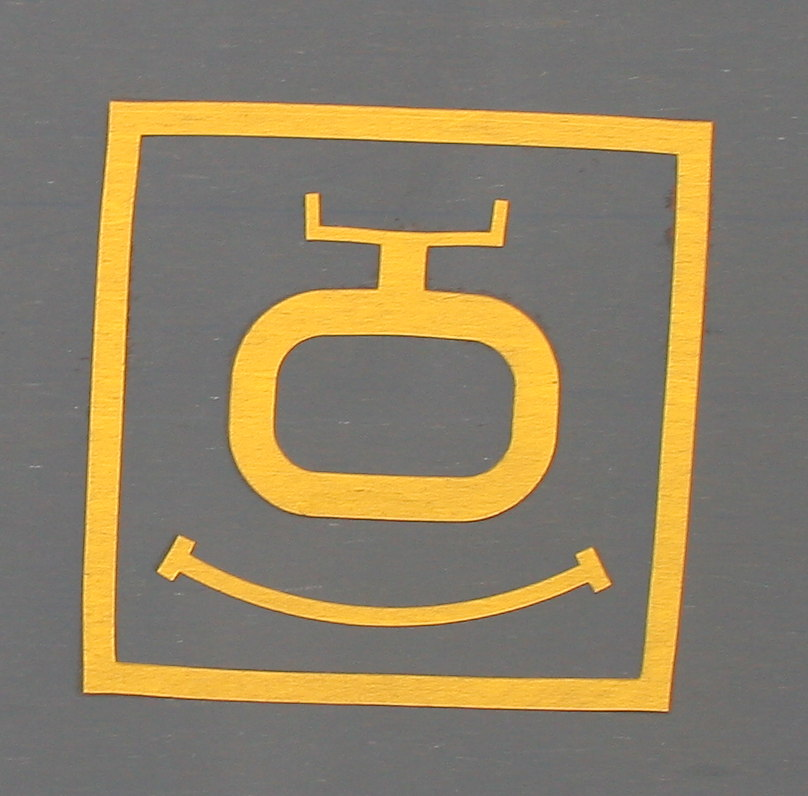
\includegraphics[width=2.5cm]{skryptkierownik-img/skryptkierownik-img031.jpg} & Mostkowanie hamulca bezpieczeństwa\\
	\hline
	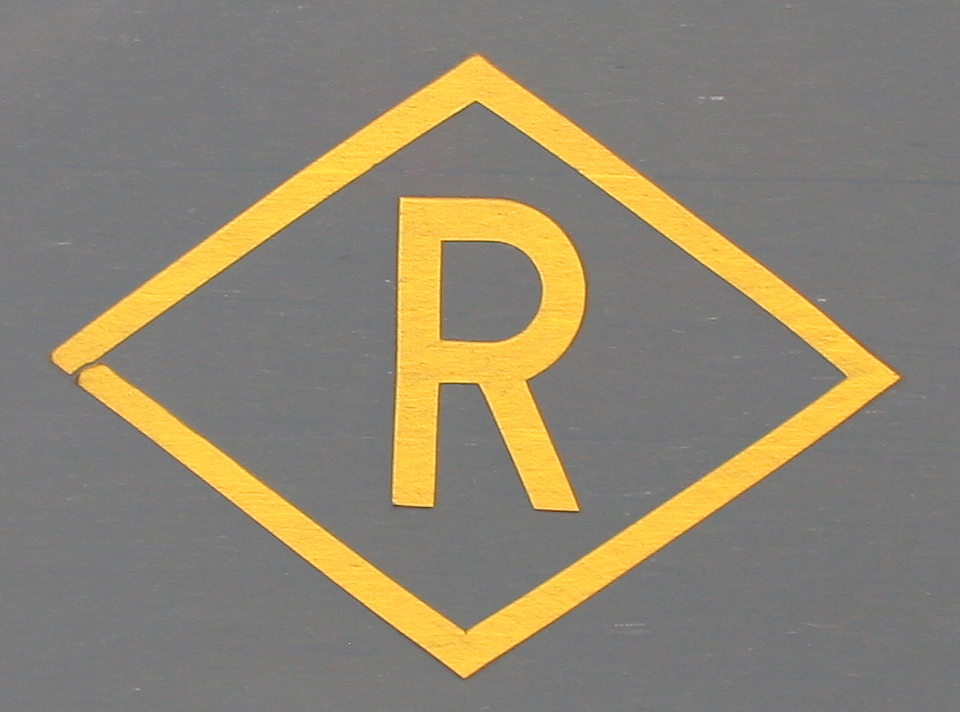
\includegraphics[width=2.5cm]{skryptkierownik-img/skryptkierownik-img032.jpg} & na nastawieniu R ("pospieszny") hamulec zapewnia procent masy hamującej wagonu próżnego od 150\% do 170\%\\
	\hline
\end{tabular}
\end{table*} 

\chapter{Obsługa urządzeń wagonowych}

Typowe urządzenia wagonowe to:

\begin{itemize}
	\item toaleta
	\item ogrzewanie i klimatyzacja
	\item oświetlenie
	\item drzwi
	\item hamulec bezpieczeństwa
	\item rampa/winda/podnośnik dla osób niepełnosprawnych
	\item światła końca pociągu
\end{itemize}

\begin{table*}
	\caption{Oznaczenia wyposażenia wagonowego}
	\label{tab:opisywagonowe}
	\begin{tabular}{|c|m{8cm}|}
		\hline
		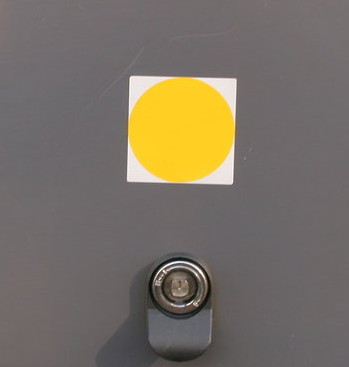
\includegraphics[width=2.5cm]{skryptkierownik-img/skryptkierownik-img035.jpg} & Złącze do wodowania\\
		\hline
	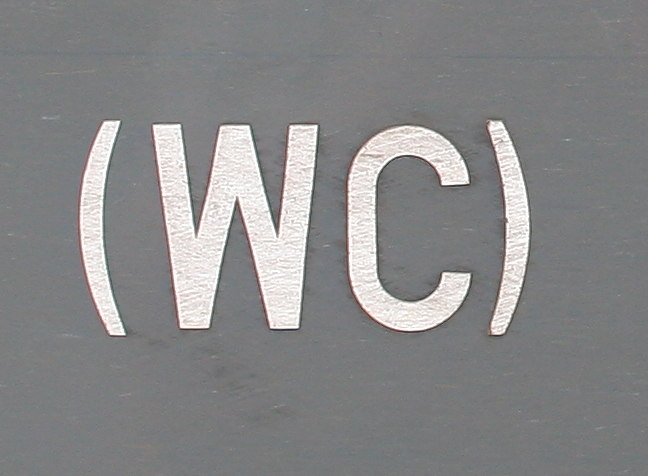
\includegraphics[width=2.5cm]{skryptkierownik-img/skryptkierownik-img036.jpg} & Wagon wyposażony w WC w układzie zamkniętym\\
	\hline
		\includegraphics[width=2cm]{skryptkierownik-img/skryptkierownik-img037.jpg} & Wagony z instalacją głośnikową, bez możliwości dołączenia zewnętrznych urządzeń\\\hline
	\end{tabular}
\end{table*}
\pagebreak
\section{Toalety}
	\begin{figure}
\subfloat{	\includegraphics[width=6cm]{skryptkierownik-img/skryptkierownik-img038.jpg}}
\subfloat{	\includegraphics[width=6cm]{skryptkierownik-img/skryptkierownik-img039.jpg}}
	\caption{Dostęp do sterownika toalety EN75}
\end{figure}
	W pojazdach serii \textbf{EN75 Stadler Flirt} toaleta znajduje się w członie C. W toalecie, bezpośrednio przy wejściu, nad koszem na śmieci znajduje się sterownik WC. Pokrywa otwierana kluczem konduktorskim oraz kluczem patentowym z pojazdu przeznaczonym dla kierownika pociągu. Na sterowniku znajdują się opisane klawisze do wykonania miękkiego resetu, płukania serwisowego (twardy rewers), opróżniania mrozowego przewodów,etc.

W słupku bocznym na końcu wagonu w którym znajduje się toleta pod pokrywą opisaną symbolem CPX1 znajdują się bezpieczniki klimatyzacji, oświetlenia wagonu, oraz zasilania WC.

\begin{figure}
		\includegraphics[width=10cm]{skryptkierownik-img/skryptkierownik-img040.jpg}
		\caption{EN75 - Wnętrze szafki. Po prawej stronie widoczne bezpieczniki - w górnym rzędzie znajdują się bezpieczniki WC}
\end{figure}
\begin{figure}
\subfloat{\includegraphics[width=5.5cm]{skryptkierownik-img/skryptkierownik-img055.png}}
\subfloat{\includegraphics[width=5.5cm]{skryptkierownik-img/skryptkierownik-img056.jpg}}
	\caption{Elf 2 - Z lewej lokalizacja sterownika w luku rewizyjnym, z prawej sterownik}	
\end{figure}
W pojazdach serii \textbf{Elf 2} toaleta znajduje się w członie A (w 34WEa), lub C (w pozostałych pojazdach trzy i czteroczłonowych) Aby wykonać uzdatnienie WC należy otworzyć kluczem konduktorskim i kluczem patentowym zamki na zewnątrz WC od strony przejścia. W środkowej części otwartej przestrzeni znajduje się sterownik WC z czterema przyciskami. Wykonanie odpowiedniej operacji polega na \textbf{równoczesnym }wciśnięciu odpowiednich przycisków. Informacja o kombinacji przycisków znajduje się na wewnętrznej części pokrywy. Dla wykonania “twardego rewersu” należy dodatkowo potwierdzić operację (wskazanym przyciskiem).
\begin{figure}
	\includegraphics[width=10cm]{skryptkierownik-img/wc-elf2.png}
	\caption{Kombinacje przycisków na sterowniku WC w pojazdach Elf2}
\end{figure}
\begin{marginfigure}
	\includegraphics[width=5.5cm]{skryptkierownik-img/skryptkierownik-img057.jpg}
	\caption{Sterownik WC toalet w pojazdach produkcji Newagu}
\end{marginfigure}
W pojazdach produkcji firmy Newag (EN57AKŚ, EN71AKŚ, 35WE, 36WEa) sterownik toalety znajduje się na zewnętrznej stronie ściany toalety. Pod pokrywą zamykaną kluczem konduktorskim można dokonać płukania (rewersu) „miękkiego” lub serwisowego. Dodatkowo, powyżej sterownika, znajduje się przełącznik wyłączenia zasilania toalety, przy pomocy którego możemy na przykład znieść blokadę drzwi.

\begin{figure}
	\includegraphics[width=5.5cm]{skryptkierownik-img/skryptkierownik-img058.jpg}
	\caption{Lokalizacja sterownika toalety w pojazdach firmy Newag}
\end{figure}

W pojazdach typu EN76 i 27WEb sterownik toalety znajduje się wewnątrz WC, za lustrem otwieranym przy pomocy klucza konduktorskiego. Sposób sterowania jest analogiczny do tego z pojazdów typu EN57AKŚ (przyciski dla płukania wstecznego i płukania serwisowego).

\section{Podnośnik dla osób niepełnosprawnych}
W pojazdach EN75 podnośnik znajduje się w członie C, obok toalety. Aby użyć podnośnika dla osób niepełnosprawnych, należy w pierwszej kolejności otworzyć kluczem kierownika pociągu zamek znajdujący się na obudowie zewnętrznej. Otworzyć drzwi wagonu, następnie pociągnąc za klamkę (pokrywę), i ustawić podnośnik równolegle do drzwi wejściowych – w tym czasie zamknie się stopień wejściowy i uruchomi sygnał ostrzegający.
Następnie wypchnąć płytę podnośnika poza pojazd (można wspomagać się dźwignią po prawej stronie), aż do pozycji leżącej. W kolejnym kroku otworzyć pokrywy/ograniczniki. Sterowanie podnośnikiem z przenośnego pilota czarnymi
klawiszami. Po podniesieniu rampy podnośnika z peronu spowrotem do wysokości wagonu, należy „dociągnąć” rampę przy pomocy żółtego przycisku na górnej części pilota.

Aby obsłużyć podnosnik awaryjnie należy wyłączyć zasilanie podnośnika bezpiecznikiem, następnie przekręcić śrubę pompy hydraulicznej i pociągnąć za czerwoną rączkę aby opuszczać rampę podnośnika. Następnie należy dokręcić śrubę i umieścić
we wskazanym miejscu w lewarku pompy drążek. Przy pomocy lewarka można podnieść rampę i wciągnąć ją do wagonu. Składanie rampy w odwrotnej kolejności do rozkładania.
	\begin{marginfigure}
	\includegraphics[width=5cm]{skryptkierownik-img/skryptkierownik-img041.jpg}
	\caption{Awaryjne (ręczne) sterowanie podnośnikiem}
\end{marginfigure}

W pojazdach Elf 2 podnośnik znajduje się obok toalety. Należy odblokować zamek drzwi i uchylić je, odblokować zamek
podnośnika przez pociągnięcie uchwytu do siebie. Następnie pociągnąć za uchwyt obracając podnośnik aż znajdzie się na
zewnątrz pojazdu. Po obrocie podnośnika o 180° zaskoczy zatrzask blokady jego osi obrotu blokując tym samym ruch
obrotowy.

Kolejne czynności:

\begin{itemize}
	\item opuścić platformę do poziomu.
	\item odciągnąć zatrzask i jednocześnie
	\item rozłożyć rozkładaną platformę środkową do poziomu obracając ją o
	\item 180°.
	\item odciągnąć zatrzask i jednocześnie otworzyć najazd zewnętrzny przez obrót o 90° (pozycja ta zostaje ustalona zatrzaskiem);
	\item otworzyć poręcz przez obrót o 90° (do pionu) do momentu  zatrząśnięcia rygla;
	\item odciągnąć zatrzask i jednocześnie otworzyć najazd wewnętrzny przez obrót o 90° (pozycja ta zostaje ustalona zatrzaskiem);
	\item Załączyć układ elektryczny podnośnika pokładowego przez obrót wyłącznika głównego w pole „I”.
\end{itemize}
\begin{marginfigure}
	\includegraphics[width=5cm]{skryptkierownik-img/skryptkierownik-img053.jpg}
	\caption{Lokalizacja skrytki na rampę przenośną}
\end{marginfigure}
Sterowanie platformą wykonać można zarówno z poziomu pokładu jak i peronu.

Aby przygotować podnośnik do dalszej jazdy należy wykonać następujące czynności:

\begin{itemize}
	\item wyłączyć układ elektryczny podnośnika przez obrót wyłącznika głównego w położenie „0”;
	\item złożyć najazd wewnętrzny i zewnętrzny oraz poręcz;
	\item złożyć składaną platformę środkową;
	\item zamknąć platformę podnosząc ją do pozycji pionowej;
	\item złożyć podnośnik do pozycji „do transportu”, upewnić się, że zadziałał zatrzask blokujący podnośnik;
	\item zamknąć drzwi obudowy.
\end{itemize}
W przypadku awarii pompy elektrycznej lub sterowania podnośnika można opuścić lub podnieść go w następujący sposób:
- ruch podnośnika „do góry” realizowany jest poprzez pompę ręczną (pokrętło zaworu awaryjnego wykręcone w lewo)
- ruch podnośnika „na dół” uzyskuje się przez przekręcenie (w prawo) pokrętła zaworu awaryjnego opuszczania

\begin{marginfigure}
	\includegraphics[width=5cm]{skryptkierownik-img/skryptkierownik-img054.jpg}
	\caption{Rozkładanie rampy}
\end{marginfigure}
Dodatkowo istnieje możliwość skorzystania z przenośnej rampy którą można rozłożyć na wysokich peronach, aby umożliwić wjazd wózka o własnych siłach. Rampa znajduje się w słupku bocznym drzwi na przeciwko toalety. 

W pojazdach typu AKŚ (EN57, EN71), w celu rozłożenia rampy podjazdowej dla osób niepełnosprawnych należy odkręcić kluczem konduktorskim zamek rampy, obrócić ją wokół osi do drzwi, a następnie odblokować zapadkę (pałąk zabezpieczający). Tak przygotowaną rampę wystarczy od strony peronu pociągnąć za uchwyty do rozłożenia. Składanie w odwrotnej kolejności. Uwaga! W stanowisku rampy znajduje się czujnik jej poprawnego zamknięcia który może uniemożliwić uruchomienie napędu.

\begin{figure}
\subfloat{	\includegraphics[width=6cm]{skryptkierownik-img/skryptkierownik-img060.jpg}}
	\subfloat{ \includegraphics[width=6cm]{skryptkierownik-img/skryptkierownik-img063.jpg}}
	\caption{Ogólny widok drzwi i rampy, z prawej rampa rozłożona poza pojazd}
\end{figure}


\begin{figure}
	\subfloat{	\includegraphics[width=6cm]{skryptkierownik-img/skryptkierownik-img061.jpg}}
	\subfloat{	\includegraphics[width=6cm]{skryptkierownik-img/skryptkierownik-img062.jpg}}
	\caption{Zamek zabezpieczający rampę, Pałąk zabezpieczenia}
\end{figure}

\section{Drzwi}
W pojazdach EN75, EN76, 27WEb w dolnej części skrzydła drzwi znajduje się zamek na klucz konduktorski który pozwala na wyłączenie/odcięcie sterowania drzwi. W pojazdach 21WEa, 22WEd, 34WEa w lewej ściance znajduje się zamykana na klucz konduktorski oraz zamek (klucz kierownika pociągu) szafa sterownika drzwi.
	\begin{marginfigure}
		\includegraphics[width=6cm]{skryptkierownik-img/skryptkierownik-img048.jpg}
		\caption{Elf2 - Przełączniki sterownika drzwi}
	\end{marginfigure}

Pierwszy od strony lewej przełącznik służy do resetu (pozycja podstawowa opisana jako “0”, chwilowe przełączenie na pozycję “1” spowoduje zresetowanie sterownika), środkowy przełącznik stopnia (w pozycji “0” - podstawowa, “1” - ręczne chowanie stopnia, “2” - stopień wyłączony). Prawy, czerwony przycisk jest przyciskiem serwisowym, który spowoduje natychmiastowe otwarcie drzwi, np. w przypadku awarii??.

Po zatrzymaniu pojazdu V=0km/h, istnieje możliwość otwarcia pierwszej pary drzwi wraz ze stopniem, aby otworzyć drzwi należy posłużyć się kluczem kierownika pociągu przekręcając w prawo przełącznik widoczny na prawym zdjęciu – po przekręceniu łącznik powraca w pierwszą pozycję). Zamknięcie wykonujemy powtarzając operację.
	\begin{figure}
		\subfloat{\includegraphics[width=4cm]{skryptkierownik-img/skryptkierownik-img049.png}}
		\subfloat{\includegraphics[width=4cm]{skryptkierownik-img/skryptkierownik-img050.jpg}}
		\subfloat{\includegraphics[width=4cm]{skryptkierownik-img/skryptkierownik-img051.jpg}}
		\caption{Lokalizacja urządzeń sterowania drzwi Elf2. W lewym portalu przełącznik otwierania służbowego drzwi, po stronie prawej Hamulec bezpieczeństwa i awaryjne otwieranie drzwi}
	\end{figure}

Po prawej stronie drzwi znajdują się hamulec bezpieczeństwa oraz dźwignia awaryjnego otwierania drzwi (bez zasilania). W celu zahamowania awaryjnego należu silnie pociągnąć rączkę hamulca w dół, aż do zerwania plomby. Dioda sygnalizuje użycie hamulca. Aby powrócić do pozycji zasadniczej, należy przekręcić kluczem konduktorskim, jednocześnie dociskając
rączkę hamulca ku górze. Poniżej po prawej stronie znajduje się interkom umożliwiający łączność z maszynistą.
W obudowie nad drzwiami wejściowymi do pojazdu znajduje się trzpień blokady drzwi, którego przekręcenie kluczem konduktorskim spowoduje wyłączenie napędu drzwi i ich zablokowanie. Pod obudową znajduje się sterownik, który można zresetować przyciskiem, jeśli drzwi chwilowo zachowują się niepoprawnie.

\begin{figure}
	\includegraphics[width=12cm]{skryptkierownik-img/skryptkierownik-img059.jpg}
	\caption{Lokalizacja blokady i sterownika drzwi w pojazdach typu AKŚ}
\end{figure}
\begin{marginfigure}
	\includegraphics[width=5cm]{skryptkierownik-img/35we-drzwi.png}
	\caption{Układ elementów drzwi 35WE, cyfrą jeden oznaczone awaryjne otwieranie drzwi i wyłącznik mechanizmu, pod pokrywą oznaczoną cyfrą 2 znajduje się przełącznik resetu sterownika}
\end{marginfigure}

W pojeździe typu 35WE w prawym słupku portalu drzwi znajduje się dźwignia awaryjnego otwierania drzwi. W niej zabudowany jest zamek na klucz konduktorski który po wciśnięciu i przekręceniu powoduje wyłączenie i zablokowanie tych drzwi ze sterowania. Dodatkowo pod górną klapą, w środkowej części znajduje się wyłącznik sterownika drzwi, który w przypadku problemów należy przełączyć do drugiej pozycji na chwilę, a następnie przywrócić do pozycji podstawowej. Absolutnie nie wolno pozostawiać przełącznika w pozycji ''wyłączony''. 

\section{Światła końca pociągu}

W pojazdach serii Elf 2, oraz 35WE na wyposażeniu znajdują się przenośne, zasilane bateryjnie tarcze świateł końca pociągu. Przenośne światła końca pociągu znajdują się w wysuwanej szufladzie (Elf 2), albo w dolnej części prawej szafy (Impuls) w przedsionku kabiny sterującej A.

\begin{figure}
		\subfloat{\includegraphics[width=6cm]{skryptkierownik-img/skryptkierownik-img042.png}}
		\subfloat{\includegraphics[width=6cm]{skryptkierownik-img/skryptkierownik-img043.jpg}}
		\caption{Szafa w przedsionku kabiny maszynisty, miejsce przechowywania świateł końca pociągu}
\end{figure}
Dodatkowo w pojazdach typu Elf 2, aby zamontować je na miejscu do tego przeznaczonym należy wykręcić kluczem konduktorskim śrubę zabezpieczającą, a następnie wysunąć zaślepkę, a potem umieścić w tym miejscu wspornik świateł. Następnie we wsporniku umieścić światło. W pozostałych pojazdach tarcze sygnałowe końca pociągu montuje się w stałym wsporniku, na czole.

\begin{figure}
\subfloat{\includegraphics[width=6cm]{skryptkierownik-img/skryptkierownik-img044.png}}
\subfloat{\includegraphics[width=6cm]{skryptkierownik-img/skryptkierownik-img045.jpg}}\\
\subfloat{\includegraphics[width=6cm]{skryptkierownik-img/skryptkierownik-img046.jpg}}
\subfloat{\includegraphics[width=6cm]{skryptkierownik-img/skryptkierownik-img047.jpg}}
\caption{Miejsce montażu wspornika, Wspornik sygnału Pc5, szfka pod fotelem}
\end{figure}

\section{Podsumowanie}
\begin{tcolorbox}[colback=black!5!white,colframe=green!75!black,width=18cm,title=Podsumowanie rozdziału]
	\begin{enumerate}
	\item Litera E namalowana na pojeździe oznacza:
	\begin{enumerate}
		\item Pojazd z przetwornicą statyczną,
		\item Pojazd z hamulcem elektrodynamicznym,
		\item Pojazd z hamulcem elektropneumatycznym.
	\end{enumerate}	
	\item Jakie zadanie w układzie hamulcowym wagonu spełnia zawór rozrządczy:
	\begin{enumerate}
		\item Uniemożliwia zablokowanie kół podczas hamowania,
		\item Steruje pracą układu hamulcowego wagonu,
		\item Reguluje ustawienie wstawek hamulcowych.
	\end{enumerate}
	\end{enumerate}
\end{tcolorbox}

\chapter{Wykonywanie szczegółowej i uproszczonej próby hamulca}

Próba hamulca ma na celu stwierdzenie sprawności hamulca zespolonego (pneumatycznego) pociągu. Należy sprawdzić ponadto działanie hamulca elektropneumatycznego. Jeśli pociąg kursuje na hamulcach ręcznych sprawdza się działanie tych hamulców. Potwierdzeniem przeprowadzenia próby hamulca jest karta prób hamulca. Drużynie trakcyjnej nie wolno uruchomić pociągu, jeśli nie dysponuje ona dokumentem potwierdzającym wykonanie, z pozytywnym wynikiem, wymaganej próby hamulca.
Karta próby hamulca po wykonaniu próby i wypełnieniu musi znajdować się w czynnej kabinie maszynisty.

W przypadku pociągu zestawionego z pojazdu kolejowego z napędem, składającego się z jednego lub wielu członów, wyposażonego w\textbf{ hamulce tarczowe}, posiadającego nierozłączalny w normalnej eksploatacji główny przewód hamulcowy oraz manometry lub wskaźniki wskazujące ciśnienie powietrza w cylindrach hamulcowych na wszystkich wózkach jezdnych i sygnalizację stanu zahamowania i odhamowania pojazdu kolejowego w kabinie sterowniczej, dopuszcza się jednoosobowe wykonywanie \textbf{uproszczonej} próby hamulca przez \textbf{maszynistę} na podstawie tych wskazań. W spółce Koleje Śląskie próbę taką obowiązkowo wykonuje maszynista.
\begin{marginfigure}
	\includegraphics[width=5cm]{skryptkierownik-img/manometry-odhamowane.jpg}
	\caption{Manometry na pulpicie maszynisty EN76 w stanie odhamowanym. Wskazówka czerwona odnosi się do przewodu głównego, żółta do przewodu zasilającego}
\end{marginfigure}
\textbf{Szczegółową próbę hamulca} należy wykonać: 
\begin{itemize}
	\item przed wyprawieniem pociągu ze \textbf{stacji początkowej}; 
	
	\begin{itemize}
		\item odstępstwo od tej zasady może być stosowane dla pociągu, który po przybyciu na stację jest wyprawiony w dalszą
		drogę bez przeformowania lub bez naprawy urządzeń hamulcowych pod warunkiem, że przy tym składzie co najmniej jeden raz
		w ciągu poprzedzających \textbf{24 godzin} była wykonywana szczegółowa próba hamulca,\underline{ wtedy należy przeprowadzić \textbf{uproszczoną próbę hamulca}}; 
	\end{itemize}
	\item na stacjach wyznaczonych w rozkładzie jazdy pociągów;
	\item gdy urządzenia hamulcowe w składzie pociągowym lub w pociągu \textbf{nie były} \textbf{zasilane} sprężonym powietrzem \textbf{dłużej niż 12 godzin}; 
	\item po zmianie składu pociągu, jeżeli doczepione pojazdy kolejowe stanowią \textbf{więcej niż 50 \% masy brutto składu pociągu}; nie jest wymagana szczegółowa próba hamulca, pod warunkiem, że włączane pojazdy kolejowe znajdowały się w pociągach, w których co najmniej jeden raz w ciągu poprzedzających 24 godzin była wykonywana szczegółowa próba hamulca;
	
	\item jeżeli podczas uproszczonej próby hamulców stwierdzono, że hamulec jednego z dwóch ostatnich dwóch wagonów lub innych pojazdów kolejowych \textbf{nie hamuje lub nie odhamowuje}; 
	\item jeżeli maszynista stwierdzi nie działanie lub nie jest pewny prawidłowego działania hamulców (na każde żądanie maszynisty); 
	\item po przeładowaniu głównego przewodu hamulcowego pociągu powyżej \textbf{0,55MPa} i opróżnieniu komór i zbiorników sterujących za pomocą odluźniaczy.
\end{itemize}

\underline{Próba szczegółowa hamulca zespolonego pociągu polega na}: 
\begin{marginfigure}
	\includegraphics[width=5cm]{skryptkierownik-img/manometry-zahamowane-ep.jpg}
	\caption{Manometry cylindra hamulcowego w EN76 w czasie hamowania}
\end{marginfigure}
\begin{itemize}
	\item upewnieniu się że skład jest zabezpieczony przed zbiegnięciem, a hamulec \textbf{ręczny} odhamowany.
	\item skontrolowaniu we wszystkich pojazdach włączonych do składu pociągu połączeń sprzęgów i nastawień hamulca oraz sprawdzeniu na końcu pociągu czy w przewodzie głównym znajduje się sprężone powietrze i pomiarze ciśnienia tego powietrza (w EZT pomiar ciśnienia na manometrach w tylnej kabinie), 
	\item sprawdzeniu szczelności układu pneumatycznego hamulca w stanie zahamowanym (na manometrach w tylnej kabinie, spadek o mniej niż 0,05MPa w ciągu 5 minut), 
	\begin{figure*}
	\subfloat{\includegraphics[width=7cm]{skryptkierownik-img/skryptkierownik-img033.jpg}}
	\subfloat{\includegraphics[width=7cm]{skryptkierownik-img/skryptkierownik-img034.jpg}}
	\caption{Cylinder hamulcowy w stanie odhamowanym/zahamowanym}
\end{figure*}

	\item sprawdzeniu, czy w składzie pociągu hamują wszystkie wagony z czynnym hamulcem zespolonym, (sprawdzenie czy wstawki hamulcowe zostały dociśnięte do kół, oraz czy tłoki cylindrów hamulcowych wysunęły się (ok. 14cm), a jeśli wagony te mają hamulec tarczowy - czy wskaźniki pokazują zahamowanie), 
	
	\item sprawdzeniu, czy w składzie pociągu luzują hamulce wszystkich pojazdów z czynnym hamulcem zespolonym, (sprawdzenie czy wstawki hamulcowe odsunęły się od kół, oraz tłoki cylindrów hamulcowych wsunęły się w całości do cylindra, a jeśli wagony te mają hamulec tarczowy - czy wskaźniki pokazują odhamowanie)
	\marginnote{Ciiiilinder ;$)$ }
	\item należy wykonać ponownie procedurę dla hamowania hamulcem elektropneumatycznym.
	\item sprawdzeniu, czy pod względem rozmieszczenia pojazdów z czynnym hamulcem zespolonym skład pociągu jest prawidłowo zestawiony.

Próbę szczegółową wykonujemy z tej kabiny, z której będzie prowadzony pierwszy pociąg.	
\end{itemize}
\textbf{Uproszczoną próbę hamulców} należy wykonać w pociągu, w którym po dokonaniu próby szczegółowej:
\begin{itemize}
	\item nastąpiło zamknięcie lub otwarcie, nawet częściowe lub chwilowe, \textbf{przewodu głównego hamulca}, w którymkolwiek miejscu pociągu, z wyjątkiem zaworu maszynisty w czynnej kabinie sterującej i innych urządzeń na pojeździe trakcyjnym powodujących samoczynne hamowanie; w przypadku dołączenia pojazdów kolejowych do pociągu wykonuje się próbę uproszczoną hamulców pociągu, a pojazdy kolejowe dołączone poddaje się takim badaniom, jak podczas próby szczegółowej hamulca; badania te nie są wymagane w przypadku dołączenia pojazdów kolejowych na początku lub końcu pociągu i gdy włączane pojazdy kolejowe były używane w pociągach, w których co najmniej jeden raz w ciągu poprzedzających 24 godzin była wykonywana szczegółowa próba hamulca, a okres braku zasilania sprężonym powietrzem hamulców tych wagonów lub innych pojazdów kolejowych nie przekracza 12 godzin; 
	\item \textbf{wyłączono co najmniej jeden pojazd} kolejowy ze składu pociągu, 
	\item nastąpiła \textbf{zmiana przedziału} sterowniczego; 
	\item \textbf{wyłączenie zasilania sprężonym powietrzem} urządzeń hamulcowych w pociągu trwało do \textbf{12 godzin}; 
	\item szczegółowa próba hamulców była wykonana przy użyciu sieci stałej sprężonego powietrza lub innego pojazdu trakcyjnego, nieprzeznaczonego do prowadzenia tego pociągu; 
	\item nastąpiło zamknięcie lub otwarcie, nawet częściowe lub chwilowe, \textbf{przewodu zasilającego}, w którymkolwiek miejscu pociągu, którego hamulce są nastawione na przebieg hamowania \textbf{„R + Mg"};
\end{itemize}



\underline{Uproszczoną próbę hamulca wykonuje się w sposób następujący:} 
\begin{itemize}
	\item pracownik znajdujący się za ostatnim pojazdem pociągu: stwierdza, przez kilkukrotne otwieranie i zamykanie kurka końcowego przewodu głównego na końcu pociągu, że w przewodzie głównym znajduje się sprężone powietrze, a jeżeli jest to niemożliwe, sprawdza wskazanie manometru w tylnej kabinie maszynisty: 
	\begin{itemize}
		\item zamyka kurek, 
		\item upewnia się, że ostatni pojazd jest w stanie odhamowanym, 
		\item podaje do czoła pociągu sygnał Rh1 "Zahamować", 
	\end{itemize}
\begin{marginfigure}
	\includegraphics[width=6cm]{skryptkierownik-img/skryptkierownik-img069.png}
	\caption{Rh1 i Rhs1 Zahamować}
\end{marginfigure}
	\item maszynista po odebraniu sygnału Rh1 "Zahamować" wykonuje hamowanie służbowe, 
	\item pracownik dokonujący próby hamulca sprawdza czy wstawki hamulcowe \textbf{dwóch ostatnich pojazdów} są dociśnięte do kół, oraz czy tłoki cylindrów hamulcowych wysunęły się, a jeśli wagony te mają hamulec tarczowy - czy wskaźniki pokazują stan zahamowania, 
	\item po stwierdzeniu, że w sprawdzanych wagonach hamulec zahamował prawidłowo, pracownik wykonujący próbę podaje do czoła pociągu sygnał Rh2 "Odhamować",
\begin{marginfigure}
	\includegraphics[width=6cm]{skryptkierownik-img/skryptkierownik-img067.png}
	\caption{Rh2 i Rhs2 Odhamować}
\end{marginfigure}

	\item dokonujący próby sprawdza czy wstawki hamulcowe ostatnich dwóch pojazdów odsunęły się od kół, oraz czy tłoki cylindrów hamulcowych wsunęły się, a jeśli wagony te mają hamulec tarczowy - czy wskaźniki pokazują odhamowanie; 
	\item należy wykonać ponownie procedurę dla hamowania hamulcem elektropneumatycznym.
	\item jeśli hamulce dwóch ostatnich wagonów zahamowują i odhamowują poprawnie, to dokonujący próbę podaje do czoła pociągu sygnał Rh3 "Hamulce działają poprawnie".
	
\begin{marginfigure}
		\includegraphics[width=6cm]{skryptkierownik-img/skryptkierownik-img068.png}
		\caption{Rh3 i Rhs3 Hamulce działają poprawnie}
\end{marginfigure}

\end{itemize}

\section{Sygnały podawane przy próbie hamulca}

W celu nawiązania łączności między pracownikami wykonującymi próbę hamulca zespolonego pociągu i zapewnienia właściwej organizacji przeprowadzenia prób, stosuje się sygnały:

Rh1 i Rhs1 Zahamować
Rh2 i Rhs2 Odhamować
Rh3 i Rhs3 Hamulce działają poprawnie

W przypadku złej widoczności spowodowanej warunkami atmosferycznymi lub innymi (np. łuk toru), przy dokonywaniu prób hamulców w miejscach realizowanych budów, stacjach nie posiadających stałych urządzeń sygnalizacyjnych obsługa pociągu, powinna współdziałać w przekazywaniu sygnałów ręcznych. Dopuszcza się możliwość potwierdzania podawanych sygnałów przez radiotelefon przenośny i przewoźny, podczas dokonywania próby hamulca poza komendami przekazywanymi przez radiotelefon, powinno się sygnały przekazywać ręcznie.

\begin{tcolorbox}[colback=black!5!white,colframe=white!55!black,title=Pytania testowe]
	\begin{enumerate}
		\item Szczegółową próbę hamulca należy wykonać:
		\begin{enumerate}
			\item Gdy urządzenia hamulcowe w składzie pociągowym lub w pociągu nie były zasilane sprężonym powietrzem dłużej niż 12 godzin,
			\item Gdy urządzenia hamulcowe w składzie pociągowym lub w pociągu nie były zasilane sprężonym powietrzem krócej niż 12 godzin,
			\item Gdy urządzenia hamulcowe w składzie pociągowym lub w pociągu nie były zasilane sprężonym powietrzem dłużej niż 2 godziny.
		\end{enumerate}
		\item Szczegółowa próba hamulca nie jest wymagana po zmianie składu pociągu o więcej niż 50\% masy brutto, jeżeli:
		\begin{enumerate}
			\item Włączane pojazdy kolejowe znajdowały się w pociągach, w których co najmniej jeden raz w ciągu poprzedzających 24 godzin była wykonywana szczegółowa próba hamulca,
			\item Urządzenia hamulcowe w doczepianym składzie nie były zasilane sprężonym  powietrzem ponad 12 godzin,
			\item Urządzenia hamulcowe w doczepianym składzie były naprawione przez rewidenta.
		\end{enumerate}
		\item Pociąg pasażerski, który zmienia kierunek jazdy na stacjach pośrednich,  winien    być zestawiony w taki sposób, aby:
		\begin{enumerate}
			\item Ostatnie dwa wagony posiadały sprawny hamulec zespolony, 
			\item Pierwszy i ostatni wagon posiadał sprawny hamulec zespolony,
			\item Dwa pierwsze i dwa ostatnie wagony posiadały sprawny hamulec zespolony.
		\end{enumerate}
	\end{enumerate}
\end{tcolorbox}

\chapter{Obliczanie rzeczywistej oraz wymaganej masy hamującej}
Za miarę skuteczności hamulców pociągu przyjmuje się wyrażony w procentach stosunek masy hamującej pociągu do masy pociągu (tzw. masy ogólnej),
nazywany procentem masy hamującej. Rozróżniamy:
\begin{enumerate}
	\item procent wymaganej masy hamującej, oznaczany P\textsubscript{w} , podawany dla każdego pociągu w rozkładzie jazdy,
	\item procent rzeczywistej masy hamującej, oznaczany P\textsubscript{r} , wynikający z rzeczywistej masy hamującej i masy ogólnej zestawionego pociągu.
\end{enumerate}

\textbf{Procent wymagany masy hamującej} odczytujemy z wewnętrznego rozkładu jazdy pociągu. Znajduje się on w ostatniej kolumnie, w mianowniku, oznaczony symbolem \%. 
\begin{figure*}
	\includegraphics[width=16cm]{skryptkierownik-img/skryptkierownik-img065.png}
	\caption{Informacja o \% wymaganej masy hamującej w w.r.j.}
	\label{fig:pw}
\end{figure*}

Następnie możemy wyliczyć \textbf{Masę hamującą wymaganą} z następującego wzoru:
\[  M_{w}=\frac{M_{o}*P_{w}}{100} \label{wzr:mhw}  \]
\marginnote{Instrukcja K-2, Rozdział VIII, \S.28, ust.4, p.5}
Masę hamującą wymaganą po wyliczeniu zaookrąglamy w górę, do pełnej liczby.

Masa ogólna pociągu/składu (M\textsubscript{o}) to \textbf{suma mas pojazdów} kolejowych w składzie pociągu, wraz z ładunkiem. Masę składu w stanie ładownym, jeśli nie jest wskazane na pudle wagonu, należy obliczyć na podstawie masy służbowej składu (masy składu przygotowanego do drogi, z nawodowanymi toaletami, napełnionymi piasecznicami, etc.) dodając po \textbf{5 t} na wagon, zaś masę w stanie próżnym odczytujemy z pudła pojazdu (oznaczone jako \textbf{masa służbowa}). W jednym składzie pociągu mogą znajdować się zarówno pojazdy (wagon lub EZT) dostępne dla podróżnych (ładowne), jak i niedostępne dla podróżnych (próżne).

\textbf{Masa hamująca rzeczywista} elektrycznego zespołu trakcyjnego, lokomotywy lub wagonu jest wskazywana na pudle. Należy brać pod uwagę największe wartości dla hamulca pneumatycznego (jeśli urządzenie Rapid jest sprawne, to z nim). Rzeczywistą masę hamującą pociągu M\textsubscript{ hr} stanowi suma (w tonach) mas hamujących, poszczególnych pojazdów z czynnymi hamulcami, za wyjątkiem czynnych lokomotyw, z zastrzeżeniem informacji w ramce poniżej. Należy zwrócić uwagę na rozróżnienie mas hamujących w stanie próżnym i ładownym.

\begin{tcolorbox}[colback=red!5!white,colframe=red!75!black,width=18cm,title=Uwaga!]
	W pociągach
	\begin{enumerate}
		\item których rozkładowa prędkość jest większa od 120 km/h albo
		\item w których masa składu pociągu jest mniejsza niż 200 t albo
		\item w których pojazd z napędem znajduje się na końcu pociągu, a maszynista prowadzi pociąg z kabiny w wagonie sterowniczym,
	\end{enumerate}
	wlicza się:
	\begin{itemize}
		\item masę hamującą czynnych pojazdów z napędem do rzeczywistej masy hamującej pociągu M\textsubscript{hr} oraz,
		\item masę czynnych pojazdów z napędem do masy ogólnej pociągu M\textsubscript{O} ,przy czym jeśli pojazd z napędem ma wypisaną masę własną i masę służbową należy w obliczeniach uwzględniać masę służbową tego pojazdu.
	\end{itemize}
	\label{def:masa}
\end{tcolorbox}

Gdy znamy masę ogólną składu, oraz masę hamującą rzeczywistą możemy wyliczyć \textbf{Procent rzeczywisty masy hamującej} składu z następującego wzoru: 
\marginnote{Instrukcja K-2, Rozdział VIII, \S.28, ust.5}
\[  P_{r}=\frac{M_{hr}*100}{M_{os}}   \label{def:pr} \] 
gdzie P\textsubscript{r} to Procent rzeczywisty masy hamującej, M\textsubscript{hr} to Masa hamująca rzeczywista w tonach, zaś M\textsubscript{os} to masa ogólna składu. Wartość procentu rzeczywistego masy hamującej po wyliczeniu zaookrąglamy w dół.

\textbf{Procent rzeczywistej masy hamującej} składu powinien być równy lub większy niż procent wymagany masy hamującej.
\[  P_{r} \ge P_{w}   \] 

\begin{marginfigure}
	\includegraphics[width=5.5cm]{skryptkierownik-img/zmniejszenie-mhr.png}
	\caption{Jeśli dwa ostatnie wagony nie hamują lub nie odhamowowują - odstawiamy skład. Przykład środkowy dotyczy składu 3 wagonowego, przykład trzeci dotyczy składu 4 lub więcej wagonowego.}
\end{marginfigure}

\begin{tcolorbox}[colback=green!15!white,colframe=green!75!black,title=Zmiana M\textsubscript{hr} po wyłączeniu hamulca zespołu trakcyjnego - wariant 1]
	W przypadku wyłączenia hamulca w \textbf{jednym} wagonie/członie zespołu trakcyjnego masa hamująca rzeczywista składu musi być zmniejszona. W tym celu odczytujemy masę hamującą rzeczywistą całego zespołu (z pudła) a następnie:
	\begin{itemize}
		\item W składzie EZT złożonego z dwóch lub trzech wagonów masa hamująca rzeczywista składu zmniejsza się o połowę ($ \frac{1}{2}*M_{hr} $).
		\item W składzie złożonym z czterech lub więcej wagonów stosujemy wzór $ \frac{2}{3}*M_{hr} $ 
	\end{itemize}
	Jeśli hamulce w conajmniej dwóch wagonach zespołu trakcyjnego są niesprawne lub wyłączone - \textbf{pociąg nie może być wyprawiony w drogę}	
\end{tcolorbox}

\begin{tcolorbox}[colback=yellow!15!white,colframe=green!75!black,title=Zmiana M\textsubscript{hr} po wyłączeniu hamulca zespołu trakcyjnego - wariant 2]
	Jeśli wewnętrzne regulacje przewoźnika dopuszczają wyłączenie hamulca na pojedyńczych wózkach, oraz na pudle pojazdu lub w instrukcji znajdują się masy hamujące rzeczywiste poszczególnych wózków, to M\textsubscript{hr} składu jest równa sumie mas hamujących rzeczywistych wózków z czynnym hamulcem.
	\\ Inaczej mówiąc jest to masa hamująca rzeczywista całego EZT minus masa hamująca wózka z wyłączonym hamulcem.
	\[ M{hr} = M_{hrEZT} - M_{hrw1}  \] gdzie M\textsubscript{hrw1} to masa hamująca rzeczywista wózka z wyłączonym hamulcem.
\end{tcolorbox}
\begin{marginfigure}
	\includegraphics[width=5.5cm]{skryptkierownik-img/mhr-wozki.jpg}
	\caption{Masy hamujące pojedyńczych wózków EZT - na zdjęciu opisy na pudle 34WEa, liczone od strony członu A od lewej strony}
\end{marginfigure}

\begin{tcolorbox}[colback=black!5!white,colframe=white!55!black,title=Pytania testowe]
	\begin{enumerate}
		\item Jeżeli rzeczywista masa hamująca pociągu jest mniejsza od wymaganej należy:
		\begin{enumerate}
			\item Jechać z pociągiem ostrożnie,
			\item Zwiększyć obciążenie pociągu,
			\item Zmniejszyć prędkość pociągu stosownie do procentu rzeczywistej masy hamującej
		\end{enumerate}
		\item Wymagany procent masy hamującej dla danego pociągu:
		\begin{enumerate}
			\item Jest ustalony w wewnętrznym rozkładzie jazdy,
			\item Jest ustalany przez kierownika pociągu,
			\item Jest ustalany przez rewidenta taboru
		\end{enumerate}
	\end{enumerate}
\end{tcolorbox}	

\chapter{Sprzęganie i rozprzęganie taboru}

\textbf{Zabrania się} ręcznego sprzęgania i rozprzęgania pojazdów kolejowych będących \textbf{w ruchu}. Dozwolone jest natomiast dociśnięcie taboru pojazdem trakcyjnym celem jego sprzęgnięcia lub rozprzęgnięcia. Wejście pomiędzy pojazdy kolejowe lub wyjście spomiędzy pojazdów kolejowych może nastąpić, gdy pojazdy kolejowe nie są w ruchu. 

Przy wchodzeniu pomiędzy pojazdy kolejowe dla dokonania sprzęgnięcia lub rozprzęgnięcia pojazdów kolejowych należy zachować szczególną ostrożność. Wchodząc należy schylić się poniżej zderzaka, chwytając ręką za uchwyt umocowany pod zderzakiem do czołownicy pojazdu kolejowego. 

Skład manewrowy powinien być sprzęgnięty możliwie krótko (dla uniknięcia nadmiernych szarpnięć w czasie manewrów). Lokomotywę manewrową należy sprzęgnąć z pierwszym wagonem w ten sposób, aby zderzaki stykały się ze sobą. 

Przy łączeniu taboru w składzie pociągu, należy wykonywać kolejno następujące czynności: 

\begin{enumerate}
	\item założyć na hak sprzęg cięgłowy i odpowiednio go skręcić, 
	\item połączyć sprzęgi hamulcowe i zasilające, 
	\item otworzyć kurki powietrzne.
	\item połączenie elektryczne przewodem WN wykonuje \textbf{maszynista}!
\end{enumerate}
Przy rozłączaniu taboru czynności odbywają się w odwrotnym porządku, przy czym najpierw należy zamykać kurek przewodu hamulcowego od strony pojazdu trakcyjnego. Rozłączone sprzęgi hamulcowe i ogrzewcze należy założyć na wsporniki. Zamykanie kurków przewodu głównego, zasilającego, ogrzewczego, rozłączanie sprzęgów hamulcowych, zakładanie tych sprzęgów na wsporniki może być dokonywane tylko po całkowitym zatrzymaniu pojazdów kolejowych. 

Po dojeździe pojazdu trakcyjnego do przygotowanego składu pociągu, należy w pojeździe trakcyjnym usunąć wodę i zanieczyszczenia z przewodów powietrznych poprzez ich kilkukrotne, chwilowe otwarcie i zamknięcie, pamiętając o pewnym oparciu przewodu o nogę, aby nie doznać urazu.

Przy sprzęganiu pojazdów kolejowych należy zwracać uwagę na właściwe trzymanie sprzęgu. Pałąk sprzęgu należy trzymać w dolnej jego części przy śrubie rzymskiej, przestrzegając przy tym, aby palce rąk znajdowały się po zewnętrznej stronie pałąka. Zarzucanie pałąka sprzęgu na hak łączonego pojazdu kolejowego powinno być dokonywane szybko, a ręce natychmiast usunięte. Zdejmowanie pałąka sprzęgu z haka należy dokonywać w kolejności odwrotnej, zwracając przy tym uwagę, aby opuszczony sprzęg nie zranił nóg pracownika rozprzęgającego pojazdy kolejowe. Sprzęgi pojazdów kolejowych nieużyte do sprzęgania, należy podwiesić w taki sposób, że nie powinny zwisać niżej niż 140 mm ponad główkę szyny (według oszacowania wzrokowego). 

Po zakończeniu manewrów, sprzęgi nieużyte do połączenia pojazdów kolejowych należy założyć na haki zarzutowe. Sprzęganie pojazdów kolejowych należy wykonywać w taki sposób by tarcze zderzakowe powinny być lekko naciśnięte tj. od momentu styku zderzaków wykonać od jednego do maksimum dwóch obrotów śruby sprzęgu. 

Maszynista w każdym przypadku odpowiedzialny jest za należyte sprzęgnięcie obsługiwanego pojazdu trakcyjnego ze składem pociągu, połączenie sprzęgu wysokiego napięcia oraz za otwarcie kurków przewodu hamulcowego między pojazdem trakcyjnym i składem. 

\chapter{Zabezpieczenie taboru przed zbiegnięciem}

Zabezpieczenia taboru przed zbiegnięciem dokonuje się poprzez zahamowanie pojazdów kolejowych hamulcem ręcznym lub postojowym sprężynowym, a także poprzez wyłożenie płozów hamulcowych. Zabezpieczenie przy pomocy płoza należy wykonać \textbf{od strony spadku}, w sposób wskazany w regulaminie technicznym stacji.

Płóz hamulcowy składa się z następujących zasadniczych części:
1) podeszwy ślizgowej z jedną lub dwoma wargami; przy podeszwie ślizgowej rozróżniamy: spód ślizgowy, wierzch podeszwy, wargi i język podeszwy,
2) stopki,
3) uchwytu.

Używane płozy powinny odpowiadać typom szyn, na których są wykładane. W zależności od typów szyn stosowane są płozy dwuwargowe o różnej szerokości powierzchni ślizgowej (rozstępu pomiędzy wargami), a mianowicie:
\begin{marginfigure}
	\includegraphics[width=5cm]{skryptkierownik-img/ploz.jpg}
	\caption{Zestawy kołowe zabezpieczone płozem}
\end{marginfigure}

\begin{itemize}
	\item szerokości 64 mm, malowane na kolor \textbf{niebieski} – do szyn typu 6,
	\item typu PL1 o szerokości 73mm, malowane na kolor \textbf{czerwony} - do szyn typu S42, S49, 39, 41,
	\item typu PL2 o szerokości 78mm, malowane na kolor \textbf{żółty} - do szyn typu 8, 15, 40, S60,
	\item typu PL3 uniwersalne (wzmocnione) o szerokości 78mm, malowane na kolor \textbf{pomarańczowy} - do szyn typu 8, 15, 40, S42, S49 S60, UIC
	60, R65.
\end{itemize}

Nie wolno wykładać płoza hamulcowego:
\begin{itemize}
	\item w odległości mniejszej niż 1m od złącza szynowego (styku),
	\item w łukach na zewnętrznym toku szynowym,
	\item na opornicy rozjazdu przed przylegającą do niej iglicą,
	\item przed krzyżownicą rozjazdu (zasadniczo w rozjeździe nie wykładamy),
	\item przed przejazdami kolejowo-drogowymi.
\end{itemize} 
	
	\part{Organizacja i bezpieczeństwo pracy}
	\part{Organizacja i bezpieczeństwo pracy}
\chapter{Prawa i obowiązki kierownika pociągu wynikające z regulaminu pracy}
Prawa pracownika to w szczególności:
\begin{itemize}
	\item zatrudnienie na stanowisku pracy zgodnie z umową o pracę i posiadanymi kwalifikacjami,
	\item terminowe wynagrodzenie za pracę, 
	\item odpoczynek w dniach wolnych od pracy oraz po zakończeniu pracy, 
	\item płatny urlop wypoczynkowy, 
	\item jednakowe i równe traktowanie przez pracodawcę z tytułu wypełniania jednakowych obowiązków, 
	\item wykonywanie pracy w warunkach zgodnych z zasadami bezpieczeństwa i higieny pracy.
\end{itemize}
Do obowiązków pracownika należą w szczególności:
\marginnote{Regulamin pracy, rozdział III, \S 6-12}

\begin{itemize}
	\item rzetelne i efektywne wykonywanie pracy,
	\item przestrzeganie czasu pracy i wykorzystanie go w sposób jak najbardziej efektywny, w pełni na pracę zawodową,
	\item podporządkowanie się poleceniom pracowników usuwających awarię, lub prowadzących akcję ratowniczą, czy ewakuację,
	\item dbałość o dobro i mienie pracodawcy oraz zachowywanie w tajemnicy informacji technicznych, technologicznych, handlowych lub organizacyjnych, tajemnicy przedsiębiorstwa,
	\item przestrzegania zasad współżycia społecznego.
\end{itemize}
     Pracownik zobowiązany jest zapobiegać wszystkiemu, co zagraża bezpieczeństwu ruchu kolejowego, bezpieczeństwu ludzi oraz bezpieczeństwu mienia pracodawcy. 

\chapter{Obowiązki kierownika pociągu z jedno- i wieloosobową obsadą konduktorską}

Do zadań kierownika pociągu podczas pracy, należy:
\begin{enumerate}
	\item przyjmowanie i zdawanie składu pociągu,
	\item prowadzenie na bieżąco dokumentacji pociągowej,
	\item organizowanie pracy podległej drużyny konduktorskiej
	\item nadzorowanie podległych pracowników drużyny konduktorskiej tj. konduktorów, pracowników odbywających szkolenie praktyczne i innych
	pracowników wykonujących pracę w pociągu,
	\item kontrola dokumentów przewozu i odprawa podróżnych oraz udzielanie informacji w sprawach taryfowych i rozkładu jazdy pociągów KSL,
	\item Zapewnienie podróżnym niezbędnej pomocy podczas wsiadania i wysiadania z pociągu, w tym w szczególności osobom niepełnosprawnym i osobom
	o ograniczonych zdolnościach ruchowych,
	\item zgłaszanie na stacjach początkowych gotowość pociągu do odjazdu,
	\item nadzór nad odjazdem pociągu z miejsca wyznaczonego postoju do czasu, gdy nie opuści on peronów,
	\item stały kontakt z maszynistą, a w razie potrzeby zatrzymanie pociągu,
	\item rozstrzyganie sporów pomiędzy obsługą pociągu i podróżnymi oraz pomiędzy współpodróżnymi, o ile spór pomiędzy współpodróżnymi utrudnia podróż innym osobom,
	\item wykonywanie poleceń pracowników posterunków technicznych zarządcy	infrastruktury, organów kontrolnych i zwierzchnich, mających związek
	z wykonywaną pracą. Kierownik pociągu ma prawo odmówić wykonania polecenia lub też wstrzymać jego wykonanie, jeśli wykonanie wiązałoby się ze
	stworzeniem sytuacji zagrażającej bezpieczeństwu ruchu kolejowego. Ma on w takich przypadkach również prawo uchylić takie polecenie, wydane
	podległym pracownikom,
	\item wykonywanie w razie potrzeby pracy manewrowej,
	\item nadzór nad przestrzeganiem przepisów porządkowych i stanem bezpieczeństwa w pociągu,
	\item udzielanie pierwszej pomocy w nagłych wypadkach przed przybyciem lekarza lub pogotowia,
	\item wykonywanie wymaganej próby hamulca i oględzin technicznych w przypadku braku rewidenta,
	\item w razie potrzeby sprzęganie i rozprzęganie elektrycznych zespołów trakcyjnych, jeżeli posiada stosowne uprawnienia,
	\item ustalenie długości, masy ogólnej pociągu, rzeczywistej i wymaganej masy hamującej, obliczenie największej dozwolonej prędkości jazdy pociągu (gdy rzeczywista masa hamująca jest mniejsza od wymaganej masy hamującej),
	\item bieżący nadzór nad stanem technicznym urządzeń taboru, w tym także nad działaniem SIP i rzetelnością informacji tam wyświetlanych oraz rzetelnością innych informacji zamieszczanych przez spółkę wewnątrz pojazdów,
	\item w razie potrzeby zabezpieczanie taboru przed zbiegnięciem,
	\item wdrażanie procedur postępowania w razie zaistnienia wypadku, incydentu lub wydarzenia,
	\item informowanie dyżurnego ruchu o wszelkich zauważonych nieprawidłowościach,
	\item informowanie dyspozytora Spółki i sporządzenie raportu o wszelkich zaistniałych w trakcie zmiany roboczej nieprawidłowościach.
	\item Obsługa urządzeń głośnomówiących i podawanie komunikatów dla pasażerów w standardach przyjętych przez spółkę,
	\item Informowanie podróżnych o wszelkich kwestiach związanych z przejazdem, w tym o możliwościach skomunikowania z innymi przewoźnikami kolejowymi.
\end{enumerate}
Kierownik pociągu jest pracownikiem odpowiedzialnym za obsługiwany pociąg na wyznaczonym odcinku obsługi. Kierownikowi pociągu podlegają wszyscy
pracownicy obsługujący pociąg, za wyjątkiem organów nadzoru i kontroli.

\section{Obsada pociągu}
\label{sec:obsada}
Obsadę pociągu stanowi drużyna pociągowa, w skład której wchodzi drużyna trakcyjna oraz drużyna konduktorska lub tylko drużyna trakcyjna. Jednoosobowa drużyna trakcyjna dopuszczalna jest w pociągach kursujących z prędkościami nieprzekraczającymi 130km/h \marginnote{Instrukcja K-4, \S.2, pkt.3 - zwróć uwagę poniżej}, o ile pojazd jest wyposażony w sprawne urządzenia kontrolujące czujność prowadzącego pojazd kolejowy, lub w pociągu wyposażonym w urządzenia ERTMS/ETCS poziomu 1 lub 2 na liniach kolejowych wyposażonych w urządzenia tego systemu. \marginnote{Rozporządzenie Ministra Infrastruktury z dnia 20 października 2023 r. zmieniające rozporządzenie w sprawie ogólnych warunków prowadzenia ruchu kolejowego i sygnalizacji (Dz.U.2023.2474), dopuszcza do 160km/h przy jednoosobowej drużynie trakcyjnej}

Pociągi pasażerskie przewożące pasażerów powinny mieć obsadę konduktorską składającą się co najmniej z kierownika pociągu. Pociągi pasażerskie mogą jeździć bez kierownika pociągu jeżeli zamykanie drzwi pojazdu kolejowego przy wymianie podróżnych jest zapewnione, a zamknięcie drzwi jest sygnalizowane kierującemu pojazdem kolejowym z napędem za pomocą urządzeń technicznych. 

W przypadkach uszkodzenia urządzeń CA/SHP lub urządzeń radiołączności, przy jednoosobowej obsłudze trakcyjnej, kierownik pociągu powinien zająć miejsce w kabinie sterowniczej. W przypadku braku kierownika pociągu prowadzący pojazd kolejowy ma obowiązek doprowadzić pociąg do najbliższej stacji i postępować zgodnie z przepisami wewnętrznymi przewoźnika. 

\section{Znajomość typu pojazdu kolejowego}

Kierownik pociągu przed zatrudnieniem po raz pierwszy na stanowisku kierownika, na pociągu zestawionym z nowego typu pojazdu kolejowego, winien uzyskać znajomość typu pojazdu kolejowego. Znajomość typu pojazdu kolejowego utrzymuje się przez sześć miesięcy od czasu ostatniej jazdy w charakterze kierownika. Kierownikowi pociągu \textbf{nie wolno} wykonywać obowiązków w pociągu zestawionym z taboru dla którego nie posiada aktualnej znajomości typu pojazdu kolejowego. 

\section{Znajomość linii kolejowych}

Prowadzący pojazd kolejowy lub pociąg oraz kierownik pociągu powinni znać obsługiwane odcinki linii kolejowych, na których prowadzą pociąg. Kierownik pociągu i konduktor powinien również posiadać znajomość warunków techniczno - eksploatacyjnych stacji znajdujących się na tych odcinkach. 

Jeżeli maszynista nie posiada znajomości odcinków linii na których ma prowadzić pociąg, może go prowadzić, pod warunkiem że podczas jazdy obok niego znajduje się inny maszynista lub pracownik ZLK posiadający udokumentowaną znajomość tych
odcinków (pilot). W przypadku jeśli nie ma pilota, prowadzący pojazd powinien jechać ostrożnie, nie przekraczając prędkości 40km/h. W tym przypadku prowadzącemu pojazd kolejowy lub pociąg należy wydać rozkaz pisemny „O” informujący o okolicznościach mających wpływ na bezpieczeństwo jazdy pociągu, których znajomość jest konieczna do prowadzenia pojazdu kolejowego lub pociągu na tym odcinku.

Jeżeli kierownik pociągu otrzyma polecenie jazdy na odcinku, którego warunków obsługi nie zna, powinien o tym powiadomić pracownika, który wydał mu takie polecenie, a następnie zastosować się do jego dalszych poleceń. Kierownik pociągu nie znający obsługiwanych odcinków linii kolejowych w wyjątkowych przypadkach może obsługiwać pociąg kursujący na tych odcinkach, o ile zapozna się dokładnie z dotyczącymi danymi, zawartymi w wewnętrznym rozkładzie jazdy pociągów i dodatkach do niego. O nieznajomości obsługiwanych odcinków linii kolejowych przez kierownika pociągu należy ustnie powiadomić prowadzącego pojazd kolejowy tego pociągu.

\subsection{Dokumentowanie znajomości odcinków linii}

Zasady dokumentowania uregulowane są w Uchwale Zarządu 271/2017 z 07.11.2017 dot. znajomości odcinków linii kolejowych i taboru.

Do dokumentowania znajomości odcinków linii kolejowych służą:
\begin{enumerate}
	\item Karta znajomości odcinków/linii kolejowych
	\item Wykaz nabywania znajomości odcinków linii kolejowych oraz jazd w czynnej kabinie maszynisty
\end{enumerate}


\section{Przyjęcie pociągu na stacji początkowej}
Przyjęcie pociągu i przygotowanie go do drogi na stacji początkowej i torach
postojowych przez kierownika pociągu polega na:
\begin{itemize}
	\item spisaniu pojazdów kolejowych i sporządzeniu „wykazu pojazdów kolejowych w składzie pociągu”, obliczeniu, na podstawie danych z wykazu pojazdów kolejowych w składzie pociągu, masy brutto, masy hamującej, wymaganej i rzeczywistej, ilości wagonów, długości pociągu i innych niezbędnych danych,
	\item sprawdzeniu stanu technicznego przyjmowanego składu pod względem bezpieczeństwa ruchu kolejowego i podróżnych,
	\item sprawdzeniu działania toalet, stanu czystości pojazdów oraz uzupełnienia zbiorników wodnych, stan zbiorników fekalii, zaopatrzenia w materiały eksploatacyjne, w tym materiały sanitarne (mydło, papier toaletowy, ręczniki i inne materiały, jeśli są wymagane),
	\item sprawdzeniu lub dokonaniu prawidłowego \textbf{zewnętrznego i wewnętrznego oznakowania} składu pociągu tablicami kierunkowymi i numeracyjnymi,
	prawidłowości działania elektronicznych \textbf{tablic relacyjnych} oraz weryfikacja	stanu ilościowego i technicznego tablic malaturowych,
	\item dopilnowaniu lub dokonaniu przepisowego \textbf{osygnalizowania pociągu},
	\item dopilnowaniu lub wykonaniu \textbf{oględzin technicznych pociągu} na stacjach, na których nie ma rewidentów taboru,
	\item dopilnowaniu lub wykonaniu właściwej \textbf{próby hamulca pociągu}.
\end{itemize}

W przypadku wieloosobowej drużyny konduktorskiej kierownik pociągu następujące czynności może zlecić konduktorowi:
\begin{itemize}
	\item sprawdzenie słyszalności sygnału ostrzegawczego dla pasażerów, czytelności napisów ostrzegawczych oraz sprawność działania lokalnego
	(indywidualnego) otwierania drzwi przez pasażerów,
	\item sprawdzenie wyposażenia zespołu trakcyjnego, autobusu szynowego lub wagonów pod względem zgodności z inwentarzem,
	\item odnotowanie stwierdzonych braków wyposażenia ewidencyjnego zespołu trakcyjnego lub wagonu w Książce pokładowej pojazdu trakcyjnego lub w
	Książce pokładowej wagonu,
	\item sprawdzenie stanu technicznego sprzętu p.poż., urządzeń ogrzewczych, wentylacji i klimatyzacji,
	\item sprawdzenie prawidłowości działania automatycznego zamykania oraz blokady drzwi wejściowych pojazdów,
	\item sprawdzenie, czy wszystkie nie używane sprzęgi powietrzne są podwieszone na wspornikach,
\end{itemize}

Kierownik pociągu może odmówić przyjęcia składu pociągu wyłącznie wtedy, gdy stwierdzi, że znajdujący się w nim tabor zagraża bezpieczeństwu ruchu lub podróżnych. Odmowę przyjęcia składu wraz z podaniem przyczyny, kierownik pociągu niezwłocznie zgłasza do Dyspozytury Spółki oraz odnotowuje w:
Wykazie pojazdów kolejowych, Książce pokładowej pojazdu trakcyjnego lub w Książce pokładowej wagonu, dokonując stosownego potwierdzenia podpisem
i pieczątką identyfikacyjną.

\begin{tcolorbox}
	\begin{enumerate}
		\item Czy kierownik pociągu może odmówić przyjęcia składu pociągu?
		\begin{enumerate}
			\item Nie, decyzję podejmuje rewident na podstawie oględzin technicznych,
			\item Nie, decyzję podejmuje dyspozytor taborowy,
			\item Tak, jeżeli skład pociągu zagraża bezpieczeństwu ruchu kolejowego i podróżnym.
		\end{enumerate}
		\item Czy kierownik pociągu może przebywać w kabinie maszynisty podczas jazdy pociągu?
		\begin{enumerate}
			\item Nigdy
			\item Jeżeli zostanie wezwany przez maszynistę w określonych przypadkach,
			\item Jeżeli takie polecenie otrzyma od dyspozytora.
		\end{enumerate}
	\end{enumerate}
\end{tcolorbox}

\chapter{Prowadzenie dokumentacji pociągowej}

Zgodnie z rozporządzeniem Ministra Transportu, w pociągu powinny znajdować się następujące dokumenty:
\begin{enumerate}
	\item dopuszczenie do użytkowania lub przywrócenie do eksploatacji
	\item karta próby hamulca i urządzeń pneumatycznych, zwana dalej „kartą próby hamulca”;
	\item wykaz pojazdów kolejowych w składzie pociągu;
	\item książka pokładowa wagonu – w wagonie pasażerskim i typu pasażerskiego.
\end{enumerate}

Dopuszczenie do użytkowania, oraz karta próby hamulca powinny znajdować się w czynnej kabinie maszynisty, zaś wykaz pojazdów w składzie pociągu u kierownika pociągu.

\section{Dopuszczenie do użytkowania lub przywrócenie do eksploatacji}
Dokument ten zgodnie z przepisami przyjętymi w Spółce znajduje się wewnątrz ksiązki pokładowej zespołu trakcyjnego. Wskazuje on kto i kiedy dopuścił pojazd do eksploatacji po dokonaniu czynności utrzymaniowych i naprawczych. Dokument ten wskazuje również wszelkie ograniczenia w eksploatacji, nałożone przez ECM (Spółkę) lub instytucje zewnętrzne.
\marginnote{Instrukcja K-1, \S.19-20}

\section{Karta próby hamulca i urządzeń pneumatycznych}
Przy próbie kartę próby hamulca należy wypełnić w sposób następujący:
Na stronie pierwszej kierownik pociągu lub pracownik upoważniony wypełnia następujące rubryki:
\begin{itemize}
	\item „nazwa stacji” wpisuje nazwę stacji na której wykonano próbę, wpisuje datę, imię, nazwisko i podpis wystawiającego,
	\item w pozycji 1 należy wpisać „S” dla próby szczegółowej, „U” dla próby uproszczonej,
	\item na podstawie dokumentów pociągowych i rozkładu jazdy kierownik pociągu wypełnia:
	\begin{itemize}
		\item (poz.2) Numer pociągu
		\item (poz.3) Miejsce wykonywania próby (stacja lub posterunek)
		\item (poz.4) Data i godzina \textbf{zakończenia} próby
		\item (poz.8 oraz 9) Masa ogólna składu (M\textsubscript{os}) i masa ogólna pociągu (M\textsubscript{o}) (zasady wyliczania \ref{def:masa})
		\item (poz.11) Masa hamująca rzeczywista M\textsubscript{hr}
		\item (poz. 12) Procent masy hamującej wymaganej P\textsubscript{w} - zobacz ilustrację \ref{fig:pw})
	\end{itemize}
	\item (poz. 5,6,7) na podstawie zgłoszenia osoby wykonującej próbę hamulca  wpisuje numer inwentarzowy pojazdu trakcyjnego lub kabiny/członu
	\item kierownik pociągu dokonuje obliczeń:
		\begin{itemize}
			\item (poz. 10) Masy hamującej wymaganej M\textsubscript{hw} (wzór \ref{wzr:mhw})
			\item (poz.13) Procent masy hamującej rzeczywistej P\textsubscript{r}(wzór \ref{def:pr})
		\end{itemize}
	\item (poz. 14 i 15) na podstawie wskazań manometrów w tylnej kabinie maszynisty wpisanie ciśnienia (wyłącznie po wykonywaniu próby szczegółowej, w przypadku próby uproszczonej wykreślamy te pola)
	\item po sprawdzeniu sprawności urządzeń sterowania hamulcem ep, hamulca elektrodynamicznego, urządzeń sterowania drzwiami wejściowymi, oraz innych urządzeń, takich jak toaleta w systemie zamkniętym, drzwi przejściowe, wpisuje w pola 16 - 19 słowa TAK lub NIE.
	\item w polach 20 i 21 wpisuje dwa pierwsze pojazdy za lokomotywą (lub licząc od czoła EZT) oraz dwa ostatnie pojazdy (wagony)
	\item w polu 22 wpisuje numer pojazdu z nieczynnym hamulcem umieszczonego na końcu składu.	
\end{itemize}

Na stronie nr 2 kierownik pociągu lub pracownik upoważniony wypełnia: „informację o układzie hamulcowym w składzie pociągu” w następujący sposób:
\begin{itemize}
	\item opisać stan hamulców w wagonach znakami w ten sposób, że: koniec pociągu należy oznaczyć symbolem „]”,
	pojazdy z wyłączonym hamulcem zespolonym należy oznaczyć symbolem „X”, 
	pojazdy z czynnym hamulcem ręcznym należy oznaczyć symbolem „O”.
	\item kierunek wyjazdu ze stacji pośrednich należy oznaczyć „O” zakreślając strzałkę, oraz wpisać nazwę stacji, nieczynne urządzenia zamykania drzwi w pojeździe przeznaczonym do 	przewozu osób oznaczyć symbolem „N”.
	\item wpisać numery inwentarzowe (EVN) wagonów z nieczynnym hamulcem.
\end{itemize}

W polu \textbf{podpis prowadzącego próbę} składa osoba która dokonywała sprawdzenia zahamowania i odhamowania (przy próbie uproszczonej na pojazdach z hamulcem tarczowym jest to maszynista pociągu, w pozostałych przypadkach kierownik pociągu lub rewident). 

Jeśli wykonywana była \textbf{próba szczegółowa} dla połączonego składu dwóch lub więcej EZT, należy założyć karty próby dla każdego EZT, pamiętając o poprawnym wypełnieniu informacji o numerze pojazdu z którego czynnej kabiny próbę wykonywano. Jeśli wykonywana była \textbf{próba uproszczona} dla takiego składu, wypełniamy jedynie jedną kartę próby - wyłącznie dla tego EZT z którego czynnej kabiny wykonano próbę.

\section{Wykaz pojazdów kolejowych w składzie pociągu}
W wykazie pojazdów kolejowych w składzie pociągu, zamieszcza się następujące dane:

\begin{itemize}
\item identyfikatory pojazdów kolejowych włączonych do składu pociągu;
\item długości poszczególnych pojazdów kolejowych i ich długość łączną;
\item masę poszczególnych pojazdów kolejowych (netto, tarę i brutto) i ich masę łączną;
\item masę hamującą rzeczywistą poszczególnych pojazdów kolejowych i ich łączną rzeczywistą masę hamującą;
\item stację nadania i stację przeznaczenia wraz z numerami węzłów kolejowych;
\item ewentualne informacje o przewożonych towarach niebezpiecznych wraz z numerem klasyfikacyjnym wynikającym z regulaminu RID.
\end{itemize}

Wzór wykazu pojazdów w składzie pociągu jest drukiem wstępnie wypełnionym. Należy uzupełnić pola dotyczące obsady drużyny pociągowej i odcinka obsługiwanego, typ i numer serii pojazdu, numery EVN, oraz długość pojazdu, masę netto pojazdu, masę ładunku oraz masę hamującą rzeczywistą. Następnie należy te wartości przepisać do pola H1, lub zsumować w polach H2 i H3 w przypadku jazdy ukrotnionej.

W przypadku wykazu wypełnianego na ''druku zgodnym z rozporządzeniem''\marginnote{Rozporządzenie Ministra Transportu z dnia 2 listopada 2006 r. w sprawie dokumentów, które powinny znajdować się w pojeździe kolejowym, Dz.U.2007.9.63} w górnej części formularza wprowadzamy informację o obsadzie drużyny pociągowej, jako jednostkę macierzystą należy wprowadzić identyfikator literowy przewoźnika.

W kolumnie 3, w pole państwo rejestracji wpisujemy \textbf{PL}, w kolumnie 4 wpisujemy \textbf{KSL}, dla spółki nie nadano cyfrowego identyfikatora eksploatującego pojazd kolejowy (kol. 6). Kolumny 11,12 oraz 14 należy wykreślić (przewożenie materiałów niebezpiecznych w składzie pociągu pasażerskiego jest zabronione). W kolumnie 13, przekreślić opis w nagłówku i wpisać \textbf{brutto} - a następnie w tej kolumnie wpisać masę brutto pociągu. Pozostałe pola w tej części tabeli wypełniamy zgodnie z informacjami zamieszczonymi na pudle EZT lub wagonów (masa własna pojazdu, masa ładunku, długość pojazdu, masa hamująca rzeczywista). Należy również zsumować te dane do wiersza H1 - H6.
W wierszu H1 - H6 wpisujemy parametry pociągu w następującej kolejności: Masa ogólna składu M\textsubscript{os}, Masa ogólna pociągu M\textsubscript{o}, Masa hamująca wymagana M\textsubscript{hw}, Masa hamująca rzeczywista M\textsubscript{hr}, Procent m.h. wymaganej P\textsubscript{w}, Procent m.h. rzeczywistej P\textsubscript{r}. Koniecznie pamiętaj o wpisywaniu jednostek miary (tony i procenty).

\section{Książka pokładowa wagonu}
Książka pokładowa wagonu służy do:
\begin{itemize}
\item przekazywania przez drużynę konduktorską obsłudze technicznej informacji o uszkodzeniach stwierdzonych w wagonie w czasie jego jazdy;
\item zapisu stwierdzonych przez obsługę techniczną uszkodzeń i wykonanych czynności naprawczych w wagonie w czasie postoju na stacji postojowej lub przyczyn wyłączenia wagonu z ruchu;
\item powiadamiania eksploatującego wagon o stwierdzonych uszkodzeniach, wykonanych czynnościach naprawczych lub przyczynach wyłączenia wagonu z ruchu.
\end{itemize}
Książka składa się z:
\begin{enumerate}
\item formularza meldunkowego (w kolorze białym), który wypełnia drużyna konduktorska w czasie jazdy pociągu albo obsługa techniczna na stacji \item formularza warsztatowego (w kolorze żółtym), w którym wpisy uzupełniają pracownicy obsługi technicznej na stanowiskach naprawczych;
\item formularza własnego wagonu (w kolorze różowym), który, po wykonaniu prac naprawczych lub zabezpieczających, przekazuje się z wagonem eksploatującemu pojazd kolejowy.
\end{enumerate}

\section{Książka pokładowa pojazdu z napędem}

Książka pokładowa pojazdu z napędem składa się z trzech części z których w pierwszej odnotowuje się stan urządzeń związanych z bezpieczeństwem (radiotelefon, czuwak aktywny, shp) oraz przebieg pojazdu. W części drugiej dokonuje się wpisów dotyczących dokonywanych czynności przeglądowych, oględzin technicznych, prób hamulca i wyposażenia. W części trzeciej odnotowuje się przeglądy i roboty naprawcze. W części trzeciej odnotowuje się usterki i czynności naprawcze.

\chapter{Użytkowanie urządzeń radiołączności pociągowej}

\marginnote{Instrukcja K-7, Rozdział II}

Radiołączność pociągowa służy do zapewnienia łączności pomiędzy:
\begin{enumerate}
\item dyżurnym ruchu i maszynistą pojazdu trakcyjnego znajdującego się na przyległym szlaku,
\item dyżurnymi ruchu sąsiednich posterunków - w przypadku wystąpienia całkowitej przerwy w łączności przewodowej, maszynistami pojazdów trakcyjnych znajdujących się na tym samym szlaku,
\item obchodowymi służby drogowej, eksploatacji i maszynistą pojazdu trakcyjnego jadącego po danym szlaku lub między obchodowymi i dyżurnymi
ruchu posterunków ograniczających dany szlak - wyłącznie w przypadkach zagrożenia bezpieczeństwa ruchu,
\item obsługą stanowisk kontroli urządzeń do wykrywania w czasie jazdy stanów awaryjnych taboru i maszynistami pojazdów trakcyjnych,
\item kierownikiem pociągu i maszynistą pojazdu trakcyjnego prowadzącego dany pociąg.
\item dróżnikiem przejazdowym i maszynistą w zakresie odbioru i wysyłania sygnału RADIO-STOP
\end{enumerate}

Dla sieci radiołączności pociągowej na poszczególnych liniach kolejowych przydzielone są odpowiednie kanały pracy. Przy przejeździe z jednej linii na drugą należy przełączyć radiotelefon na kanał obowiązujący na danej linii.

Numery kanałów obowiązujących na poszczególnych liniach kolejowych zarządcy infrastruktury podane są w zeszytach wewnętrznego rozkładu jazdy
pociągów i oznaczone literą ,,R'' z dodaniem cyfry oznaczającej numer kanału od 1 do 7. np.,,R6'', a punkty zmiany kanału na linii określone są wskaźnikami W28, zobacz na ilustracji \ref{fig:w28}.

Drużyna konduktorska może nawiązywać łączność z \textbf{prowadzącym pojazd kolejowy} z napędem w celu:
\begin{itemize}
	\item wymiany informacji
	\item konieczności wezwania do najbliższej stacji pomocy (policja, pogotowie itp.),
	\item podania sygnału „Gotów do odjazdu" (w zespołach trakcyjnych i wagonach silnikowych). W tym celu należy postępować zgodnie
	z zasadami podanymi w § 7.
\end{itemize}
\marginnote{Instrukcja Ir-5, \S.11, ust.3}
W przypadku zagrożenia bezpieczeństwa ruchu lub potrzeby \textbf{skomunikowania pociągów} pasażerskich drużyna konduktorska może nawiązać łączność bezpośrednio z \textbf{dyżurnym ruchu}. 

W przypadku korzystania z radiotelefonu przewoźnego aby nawiązać łączność z dyżurnym ruchu, należy wykorzystać przyciski wywołania/blokady szumu ZEW3. W przypadku łączności z innym pociągiem należy użyć przycisku ZEW1. 

W przypadku zaistnienia nagłego zagrożenia bezpieczeństwa ruchu, bezpieczeństwa podróżnych na linii wyposażonej w radiotelefoniczną łączność
pociągową, należy zastosować alarmowe zatrzymanie ruchu pociągów przez nadanie sygnału ,,ALARM'' za pomocą radiotelefonu. Prócz podania sygnału
,,ALARM'' należy podjąć działania zapobiegające wypadkowi lub zmniejszające ich skutek.

Sygnał ,,ALARM'' może być nadany w sposób:
1) automatyczny,
2) słowny - gdy w radiotelefonie nie ma przycisku ,,ALARM''.

Automatyczne nadanie sygnału ,,ALARM'' uzyskuje się przez wciśnięcie i przytrzymanie przez około 10 sekund w manipulatorze przycisku oznaczonego
napisem ,,ALARM''. Spowoduje to włączenie nadajnika i cykliczne samoczynne wysyłanie sygnału alarmowego. Sygnał ten jest odbierany przez odbiorniki
wszystkich urządzeń pracujących aktualnie na tym kanale i znajdujących się w zasięgu radiotelefonu emitującego ,,ALARM'' w postaci kombinacji trzech tonów słyszanych w głośnikach urządzeń odbierających oraz urządzenia nadającego. Powoduje to natychmiastowe samoczynne zahamowanie wszystkich pociągów znajdujących się w zasięgu i wyposażonych w urządzenia systemu „Radio-Stop”, których radiotelefony odebrały sygnał ,,ALARM''. Skasowanie sygnału ,,ALARM'' należy przeprowadzić w sposób określony w instrukcji obsługi danego typu radiotelefonu. 

Odebranie sygnału ,,ALARM'' nadanego automatycznie zobowiązuje wszystkich użytkowników, którzy go odebrali do przełączenia radiotelefonu
na kanał ratunkowy (kanał nr 8 w radiotelefonach przewoźnych, kanał nr 2 w radiotelefonach stacjonarnych) w celu wyjaśnienia przyczyny nadania
tego sygnału z najbliższym dyżurnym ruchu.

W celu nadania sygnału ,,ALARM'' słownie należy wypowiedzieć do mikrofonu co najmniej pięć razy słowo ,,ALARM''.
Pracownicy, którzy usłyszeli w swoich radiotelefonach sygnał "ALARM” nadany \textbf{słownie} powinni natychmiast przerwać prowadzone rozmowy.
Wyjaśnienie przyczyn jego nadania dokonuje się na kanale, \textbf{na którym nadany został} ten sygnał.

Prowadzący pojazdy kolejowe z napędem i pracownicy wyposażeni w radiotelefony przenośne, po usłyszeniu sygnału ,,ALARM'' zobowiązani są
natychmiast zatrzymać pojazd kolejowy, o ile nie nastąpiło to już samoczynnie.

Istnieją również sieci radiołączności stacyjnej, oraz liniowej - drogowej, SOK, zasilania elektroenergetycznego, ratunkowa. W kanał sieci ratunkowej R-8 wyposażone są wszystkie radiotelefony posiadające kanały pociągowe.



\chapter{Podawanie i odbieranie sygnałów kolejowych w zakresie drużyny pociągowej}

Przed odjazdem pociągu z miejsca, w którym wyznaczono postój dla wsiadania i wysiadania podróżnych po upewnieniu się, że nie ma przeszkód do
odjazdu drużyna konduktorska podczas procedury odjazdu pociągu wykorzystuje następujące sygnały:
\begin{itemize}
	\item Rp 11 „Wsiadać” – podawany przed odjazdem pociągów pasażerskich,
	\item Rp 12 „Gotów do odjazdu” - stosuje się przed odjazdem pociągów
	z wieloosobową drużyną konduktorską,
	\item  Rp 13 „Pociąg nr..... gotów do odjazdu” - sygnał ten kierownik pociągu przekazuje słownie lub za pomocą urządzeń łączności do maszynisty; stosuje 	się go przed odjazdem pociągów zestawionych z \textbf{elektrycznych zespołów trakcyjnych} i pojazdów silnikowych (autobusów szynowych) w przypadku, gdy urządzenia do sterowania drzwiami i sygnałem dźwiękowym ostrzegającym
	podróżnych znajdują się \textbf{na pulpicie w kabinie maszynisty}, lub zamykanie	drzwi pojazdu kolejowego przy wymianie podróżnych jest zapewnione,	a zamknięcie drzwi pojazdu kolejowego jest przekazywane kierującemu	pojazdem kolejowym z napędem za pomocą urządzeń technicznych,
	\item Rp 14 „Odjazd pociągów pasażerskich” – w pociągach wyposażonych w sterowane przez kierownika pociągu urządzenia sygnałowe do dawania
	sygnału „Odjazd”; sygnał ten podaje się za pomocą tych urządzeń.
\end{itemize}

Kierownik pociągu podaje w kierunku konduktorów sygnał Rp 12, drużyna konduktorska podaje sygnał Rp 11, po upewnieniu się, że nie ma przeszkód do odjazdu pociągu, konduktorzy podają kolejno od najdalszego konduktora w kierunku kierownika pociągu sygnał Rp 12, po otrzymaniu sygnału Rp 12 od najbliższego konduktora, kierownik pociągu podaje: w kierunku maszynisty sygnał \textbf{Rp 14} na pociągach złożonych z \textbf{lokomotywy i wagonów pasażerskich}, a jeżeli kierownik pociągu znajduje się w końcu lub środku pociągu, to sygnał Rp 14 podany przez kierownika pociągu konduktorzy powtarzają kolejno w kierunku maszynisty, albo sygnał \textbf{Rp 13} na pociągach złożonych z \textbf{zespołów trakcyjnych},

\chapter{Postępowanie w razie zagrożenia bezpieczeństwa podróżnych}
Do czasu podjęcia akcji przez jednostki specjalistyczne, kierującym wszystkimi działaniami na pokładzie pojazdu jest kierownik pociągu przy ścisłej współpracy wszystkich członków personelu pokładowego. 
W celu zapewnienia możliwości identyfikacji Kierownika pociągu na miejscu zdarzenia powinien on nosić kompletne umundurowanie (jeżeli jest to możliwe założyć kamizelkę ostrzegawczą). 
W przypadku nieobecności kierownika pociągu, kierownictwo obejmuje maszynista pociągu, który ma obowiązek realizować wszystkie obowiązki Kierownika pociągu.
Zapamiętać możliwie najwięcej szczegółów odnośnie podejrzanego przedmiotu, zjawiska czy osoby/osób w celu przekazania wyczerpującego meldunku służbom ratowniczym,
W celu uniknięcia paniki w pojeździe telefoniczny meldunek o zagrożeniu należy złożyć w kabinie maszynisty w obecności maszynisty.

Na podstawie oceny zagrożenia Kierownik Pociągu wspólnie z Dyżurnym Ruchu podejmuje decyzję w zakresie sposobu dalszego postępowania. W przypadku zarządzenia ewakuacji pociągu następuje ona w lokalizacji wskazanej przez Kierownika Pociągu.
Jeżeli Kierownik pociągu uzna, że decyzje Dyżurnego ruchu w zakresie dalszego trybu postępowania są nieadekwatne do sytuacji lub stan zagrożenia wymaga podjęcia niezwłocznych działań np. ewakuacji pasażerów Kierownik pociągu przeprowadza ewakuację w wybranej przez siebie lokalizacji i informuje o tym Dyżurnego Ruchu.

Komunikat o ewakuacji pociągu przekazuje Kierownik Pociągu za pośrednictwem urządzeń
nagłaśniających lub (w przypadku braku takich urządzeń na pojeździe kolejowym) słownie - przechodząc przez skład pociągu.
Komunikat dla pasażerów winien zawierać polecenie oddalenia się od miejsca zagrożenia
względnie (jeśli pozwalają na to warunki miejscowe) ukrycia się za budynkami lub innymi obiektami w celu zminimalizowania narażenia pasażerów na skutki potencjalnego niebezpieczeństwa. Kierownik pociągu ma obowiązek sprawdzenia czy wszyscy pasażerowie opuścili skład pociągu.
\marginnote{Art. 15. ustawy Prawo Przewozowe
	\begin{enumerate}
	\item 	Podróżny jest obowiązany do przestrzegania przepisów
	porządkowych obowiązujących w transporcie.
	\item Osoby zagrażające bezpieczeństwu lub porządkowi w transporcie mogą być
	niedopuszczone do przewozu lub usunięte ze środka transportowego.
	\item Osoby uciążliwe dla podróżnych lub odmawiające zapłacenia należności za
	przewóz mogą być usunięte ze środka transportowego, chyba że naruszałoby to zasady współżycia społecznego.
	\end{enumerate}
}

Każdorazowo interwencja policji realizowana jest \textbf{na wniosek} kierownika pociągu. Podstawą do usunięcia podróżnego z pociągu jest Ustawa Prawo Przewozowe (art. 15.1) oraz Rozporządzenie Ministra Infrastruktury z dnia 23 listopada 2004 r. w sprawie przepisów porządkowych obowiązujących na obszarze kolejowym, w pociągach i innych pojazdach kolejowych z późniejszymi zmianami, w którym określone są zakazy obowiązujące na terenie kolejowym. 


\chapter{Postępowanie w razie zagrożenia bezpieczeństwa ruchu kolejowego}

\section{Cofanie, dzielenie i zabieranie częściami składu pociągu ze szlaku}

\ \ Bez pozwolenia dyżurnego ruchu nie jest dozwolone cofanie pociągu z wyjątkiem nagle grożącego niebezpieczeństwa. Po
uzgodnieniu z dyżurnym ruchu posterunku zapowiadawczego, w kierunku którego pociąg ma cofać, na pierwszym wagonie w
kierunku cofania powinien znajdować pracownik celem obserwacji toru szlakowego i zahamowania pociągu w razie potrzeby.
Drużyna trakcyjna powinna cofać pociąg ze szczególną ostrożnością, nie przekraczając prędkości 30km/h a 20 km/h przez
przejazdy kolejowo-drogowe i przejścia, które nie są obsługiwane lub zabezpieczone w inny sposób.

\ \ W przypadku nagłego niebezpieczeństwa, cofanie pociągu ze szlaku bez uzgodnienia z dyżurnym ruchu należy wykonać z
prędkością najwyżej 5 km/h, pod warunkiem że w odległości drogi hamowania pociąg będzie poprzedzał właściwy pracownik z
przyborami sygnałowymi i że widoczność nie jest mniejsza niż 100m.

Bezwzględnie nie wolno cofać pociągu jeśli:

\begin{enumerate}
\item Pociąg jedzie bez drużyny konduktorskiej
\item Na szlaku z wieloodstępową (samoczynną) blokadą liniową, jeśli nie otrzymano pozwolenia dyżurnego ruchu
\item W czasie gdy widoczność jest mniejsza niż 100m, a nie uzgodniono z dyżurnym ruchu
\item jeżeli pociąg jedzie na jednotorowym odcinki linii kolejowej bez obsady stacji i mijanek i bez urządzeń sterowania
zdalnego, jeśli nie otrzymano pozwolenia dyżurnego ruchu odcinkowego.
\end{enumerate}
Cofany pociąg należy zatrzymać na 100 m przed semaforem odstępowym jeśli nie podawany jest sygnał do mnie, przed
urządzeniem sygnałowym ważnym dla cofanego pociągu, obok semafora wjazdowego znajdującego się przy sąsiednim torze z
prawej strony w kierunku cofania, lub w odległości 100 m przed pierwszym rozjazdem na drodze cofanego pociągu.

Jeżeli po zatrzymaniu pociągu drużyna stwierdzi że część pociągu może dalej jechać, należy powiadomić dyżurnych ruchu tylnego ( w pierwszej kolejności) i przedniego posterunku zapowiadawczego. Po otrzymaniu wiadomości o podzieleniu lub rozerwaniu pociągu na szlaku dyżurny ruchu zamyka tor szlakowy. Pozostającą na szlaku część pociągu należy zahamować i jeżeli to możliwe, strzec.

Przed odjazdem części pociągu ze szlaku należy dla niej wykonać próbę hamulca. Na odjeżdżającej części pociągu nie można umieszczać sygnałów końca pociągu, należy zanotować numer ostatniego wagonu, aby sprawdzić czy ta część pociągu dojechała do stacji w całości.

O zbliżaniu się tylko części pociągu dyżurny ruchu powinien uprzedzić zainteresowanych nastawniczych (zwrotniczych), przede wszystkim zaś posterunek nastawniczego obsługującego semafor wjazdowy od strony tego szlaku, z którego zbliża
się część pociągu.

Wjazd na stację poszczególnych części pociągu następuje na zasadach podanych dla ruchu po torze zamkniętym.Po pozostałą na szlaku część pociągu należy wysłać lokomotywę z tą samą drużyną, która przyprowadziła na stację część pociągu i (o
ile jest to możliwe) wysłać również odpowiedniego pracownika do pomocy.

\section{Rozerwanie pociągu na szlaku i zbiegnięcie wagonów}

Po zatrzymaniu rozerwanego pociągu na szlaku należy hamulcem postojowym lub ręcznym zahamować w oderwanej części składu odpowiedni procent masy ogólnej. Po wykonaniu czynności wymienionych w ust. 1, jeżeli obsada pociągu na to pozwala, to należy przednią częścią rozerwanego pociągu dojechać do części oderwanej, a następnie obie części połączyć, wykonać próbę hamulca, wagony odhamować i jechać dalej. Gdy połączenia obu części pociągu nie można wykonać, należy niezwłocznie zawiadomić o tym dyżurnego ruchu tylnego posterunku ruchu i porozumieć się z nim co do sposobu zwolnienia toru szlakowego. Wagon z uszkodzonymi urządzeniami sprzęgowymi należy, o ile to jest możliwe, zabrać z pierwszą częścią pociągu, łącząc go z tą częścią nawet w sposób prowizoryczny.

W razie zbiegania wagonów ze stacji w kierunku szlaku, należy je wszelkimi sposobami zatrzymać, a gdy to jest niemożliwe, skierować na tor żeberkowy lub inny tor stacyjny, a gdy i to nie jest możliwe – wykoleić na wykolejnicy lub w inny sposób, np. za pomocą podkładania podkładów itp. 

Na szlaku z wieloodstępową (samoczynną) blokadą liniową nie należy cofać pociągu jadącego naprzeciw zbiegłych wagonów, lecz pociąg zatrzymać.

\chapter{Wykonanie zahamowania pociągu w kabinie maszynisty}

Przed rozpoczęciem jazdy kierownika pociągu w czynnej kabinie maszynisty - w sytuacjach określonych w rozdziale Obsada pociągu (\ref{sec:obsada}) - maszynista pojazdu powinien poinstruować o sposobach zatrzymania pojazdu, a także odpisać ten fakt w książce pojazdu trakcyjnego.

Zahamowanie pociągu w kabinie maszynisty można wykonać przy pomocy nastawnika hamowania (zaworu maszynisty), poprzez pociągnięcie tegoż nastawnika do oporu (do siebie). Istnieje również możliwość użycia przycisku awaryjnego, koloru czerwonego (tzw. grzybek) znajdującego się po obu stronach pulpitu maszynisty. W pojazdach typu EN75 (Stadler Flirt) na ściance bocznej po lewej stronie od fotela maszynisty znajduje się dźwignia awaryjnego hamowania. 

W pojeździe EN57 ze względu na brak przycisku awaryjnego, oraz budowę i lokalizację zaworu hamulcowego zahamowanie pojazdu należy wykonywać przy pomocy hamulca bezpieczeństwa znajdującego się na ścianie oddzielającej kabinę maszynisty od przedziału służbowego.
\begin{marginfigure}
	\includegraphics[width=5cm]{skryptkierownik-img/grzybek.jpg}
	\caption{Przyciski awaryjnego hamowania i awaryjnego wyłączania napędu w pojeździe EN76}
\end{marginfigure}


\chapter{Odłączanie urządzeń energetycznych pojazdu w nagłych przypadkach}

\begin{marginfigure}
	\includegraphics[width=5cm]{skryptkierownik-img/siec-jezdna.jpg}
	\caption{Elementy sieci trakcyjnej}
\end{marginfigure}
Na sieci kolejowej zarządzanej przez PKP PLK jak również częściowo na sieciach czeskiej i słowackiej, sieć trakcyjna zasilana jest napięciem 3kV prądu stałego (w praktyce ok. 2400-3600V). Najczęstsze uszkodzenia sieci trakcyjnej polegają na zerwaniu przewodu jezdnego, obniżeniu sieci trakcyjnej (np. po upadku na sieć drzewa, etc.), zerwaniu wieszaka lub wysięgnika i znajdowaniu się tych elementów poniżej przewodu jezdnego, co może doprowadzić do uszkodzenia pantografu.

Rezystancja ciała człowieka waha się w dość szerokich granicach (od kilkuset omów,, do kilkuset $k\Omega$). Składa się na nią rezystancja przejścia między urządzeniem a ciałem, rezystancja naskórka, rezystancja wewnętrzna organizmu. Przyjmuje się, że rezystancja ciała człowieka wynosi $1000\Omega$. Najgroźniejszymi z prądów rażeniowych są prądy o częstotliwościach 40 ÷ 60 Hz gdyż wywołują one migotanie komór sercowych. W związku z tym przyjmuje się że napięcia i natężenia uznawane za bezpieczne w przypadku prądu zmiennego mają o połowę niższą wartość.
\begin{marginfigure}
	\includegraphics[width=5cm]{skryptkierownik-img/strefa-niebezpieczna-trakcja-10.jpg}
	\caption{Strefa niebezpieczna wokół zerwanego przewodu jezdnego}
	\label{fig:przewod}
\end{marginfigure}
W warunkach środowiskowych, w których rezystancja ciała człowieka wynosi co najmniej 1000 Ω, przyjmuje się że napięcia dzielimy w następujący sposób:
\begin{table*}
	\begin{tabular}{|c|m{2.5cm}|m{2.5cm}|}
		\hline
		Napięcie&Przemienne& Stałe\\
		\hline
		Bezpieczne &<25V &<50V\\
		\hline
		Warunkowo bezpieczne &25V-50V &50V-100V\\
		\hline
		Niebezpieczne	&>50V	&>100V\\
		\hline
	\end{tabular}
	\caption{Napięcia bezpieczne i niebezpieczne}
\end{table*}

Strefa niebezpieczna wokół zerwanego przewodu dotykającego ziemi, szyny, lub wiszącego nad torem wynosi \textbf{10m}. W tym obszarze poruszanie się wyłącznie nie odrywając jednej z nóg, lub odrywając równocześnie obie nogi (''\textit{skacząc jak żabka}''). Jeżeli przewód trakcyjny jest zerwany i dotyka pojazdu, a nie ma innych zagrożeń, takich jak pożar, nie powinniśmy w ogóle zezwalać na opuszczanie pojazdu przez podróżnych.

Odległość bezpieczna od urządzeń zasilających i sieci trakcyjnej pod napięciem wynosi \textbf{1,4m}.
\begin{marginfigure}
	\includegraphics[width=5cm]{skryptkierownik-img/strefa-niebezpieczna-trakcja-14.png}
	\caption{Strefa niebezpieczna wokół urządzeń i przewodów sieci trakcyjnej}
	\label{fig:strefa}
\end{marginfigure}
Wszelkie prace wykonywane przy urządzeniach wysokiego napięcia takie jak uszynianie, muszą być prowadzone w asyście drugiej osoby. Kierownikowi pociągu nie wolno jednak wykonywać żadnych czynności przy urządzeniach elektroenergetycznych. Drużynie konduktorskiej nie wolno również rozpinać sprzęgu elektrycznego pomiędzy lokomotywą oraz wagonami (tą czynność może wykonywać maszynista pojazdu trakcyjnego).

Przy próbie ratowania człowieka porażonego przez prąd elektryczny, nie należy go dotykać gołymi rękoma, a jedynie probować odepchnąć (oderwać), przy pomocy drąga, lub kopnięciem. Następnie należy wyciągnąć go poza strefę niebezpieczną. Najczęściej osoba porażona przez prąd elektryczny znajduje się w stanie nagłego zatrzymania krążenia, oraz może posiadać głębokie oparzenia. Pierwsza pomoc takiej osobie polega na prowadzeniu resuscytacji krążeniowo-oddechowej, oraz w miarę możliwości użyciu AED.







	
	\backmatter
	\clearpage
	\nocite{*}
	
\end{document}